%----------------------------------------------------------------------------------------
%	PACKAGES AND OTHER DOCUMENT CONFIGURATIONS
%----------------------------------------------------------------------------------------

\documentclass[11pt]{book} % Default font size and left-justified equations

%----------------------------------------------------------------------------------------

%%%%%%%%%%%%%%%%%%%%%%%%%%%%%%%%%%%%%%%%%
% The Legrand Orange Book
% Structural Definitions File
% Version 2.0 (9/2/15)
%
% Original author:
% Mathias Legrand (legrand.mathias@gmail.com) with modifications by:
% Vel (vel@latextemplates.com)
% 
% This file has been downloaded from:
% http://www.LaTeXTemplates.com
%
% License:
% CC BY-NC-SA 3.0 (http://creativecommons.org/licenses/by-nc-sa/3.0/)
%
%%%%%%%%%%%%%%%%%%%%%%%%%%%%%%%%%%%%%%%%%

%----------------------------------------------------------------------------------------
%	VARIOUS REQUIRED PACKAGES AND CONFIGURATIONS
%----------------------------------------------------------------------------------------

\usepackage[top=3cm,bottom=3cm,left=3cm,right=3cm,headsep=10pt,a4paper]{geometry} % Page margins

\usepackage{subfigure}
\usepackage{cancel}
\usepackage{colortbl}
\usepackage{steinmetz}
\usepackage{diffcoeff}

\usepackage{graphicx} % Required for including pictures
\graphicspath{{Pictures/}} % Specifies the directory where pictures are stored

\usepackage{lipsum} % Inserts dummy text

\usepackage{tikz} % Required for drawing custom shapes

\usepackage[spanish]{babel} % English language/hyphenation

\usepackage{enumitem} % Customize lists
\setlist{nolistsep} % Reduce spacing between bullet points and numbered lists

\usepackage{booktabs} % Required for nicer horizontal rules in tables

\usepackage{xcolor} % Required for specifying colors by name
\definecolor{ocre}{RGB}{52,177,201} % Define the orange color used for highlighting throughout the book

%----------------------------------------------------------------------------------------
%	FONTS
%----------------------------------------------------------------------------------------

\usepackage{avant} % Use the Avantgarde font for headings
%\usepackage{times} % Use the Times font for headings
\usepackage{mathptmx} % Use the Adobe Times Roman as the default text font together with math symbols from the Sym­bol, Chancery and Com­puter Modern fonts

\usepackage{microtype} % Slightly tweak font spacing for aesthetics
\usepackage[utf8]{inputenc} % Required for including letters with accents
\usepackage[T1]{fontenc} % Use 8-bit encoding that has 256 glyphs

%----------------------------------------------------------------------------------------
%	BIBLIOGRAPHY AND INDEX
%----------------------------------------------------------------------------------------

\usepackage[style=alphabetic,citestyle=numeric,sorting=nyt,sortcites=true,autopunct=true,babel=hyphen,hyperref=true,abbreviate=false,backref=true,backend=biber]{biblatex}
\addbibresource{bibliography.bib} % BibTeX bibliography file
\defbibheading{bibempty}{}

\usepackage{calc} % For simpler calculation - used for spacing the index letter headings correctly
\usepackage{makeidx} % Required to make an index
\makeindex % Tells LaTeX to create the files required for indexing

%----------------------------------------------------------------------------------------
%	MAIN TABLE OF CONTENTS
%----------------------------------------------------------------------------------------

\usepackage{titletoc} % Required for manipulating the table of contents

\contentsmargin{0cm} % Removes the default margin

% Part text styling
\titlecontents{part}[0cm]
{\addvspace{20pt}\centering\large\bfseries}
{}
{}
{}

% Chapter text styling
\titlecontents{chapter}[1.25cm] % Indentation
{\addvspace{12pt}\large\sffamily\bfseries} % Spacing and font options for chapters
{\color{ocre!60}\contentslabel[\Large\thecontentslabel]{1.25cm}\color{ocre}} % Chapter number
{\color{ocre}}  
{\color{ocre!60}\normalsize\;\titlerule*[.5pc]{.}\;\thecontentspage} % Page number

% Section text styling
\titlecontents{section}[1.25cm] % Indentation
{\addvspace{3pt}\sffamily\bfseries} % Spacing and font options for sections
{\contentslabel[\thecontentslabel]{1.25cm}} % Section number
{}
{\hfill\color{black}\thecontentspage} % Page number
[]

% Subsection text styling
\titlecontents{subsection}[1.25cm] % Indentation
{\addvspace{1pt}\sffamily\small} % Spacing and font options for subsections
{\contentslabel[\thecontentslabel]{1.25cm}} % Subsection number
{}
{\ \titlerule*[.5pc]{.}\;\thecontentspage} % Page number
[]

% List of figures
\titlecontents{figure}[0em]
{\addvspace{-5pt}\sffamily}
{\thecontentslabel\hspace*{1em}}
{}
{\ \titlerule*[.5pc]{.}\;\thecontentspage}
[]

% List of tables
\titlecontents{table}[0em]
{\addvspace{-5pt}\sffamily}
{\thecontentslabel\hspace*{1em}}
{}
{\ \titlerule*[.5pc]{.}\;\thecontentspage}
[]

%----------------------------------------------------------------------------------------
%	MINI TABLE OF CONTENTS IN PART HEADS
%----------------------------------------------------------------------------------------

% Chapter text styling
\titlecontents{lchapter}[0em] % Indenting
{\addvspace{15pt}\large\sffamily\bfseries} % Spacing and font options for chapters
{\color{ocre}\contentslabel[\Large\thecontentslabel]{1.25cm}\color{ocre}} % Chapter number
{}  
{\color{ocre}\normalsize\sffamily\bfseries\;\titlerule*[.5pc]{.}\;\thecontentspage} % Page number

% Section text styling
\titlecontents{lsection}[0em] % Indenting
{\sffamily\small} % Spacing and font options for sections
{\contentslabel[\thecontentslabel]{1.25cm}} % Section number
{}
{}

% Subsection text styling
\titlecontents{lsubsection}[.5em] % Indentation
{\normalfont\footnotesize\sffamily} % Font settings
{}
{}
{}

%----------------------------------------------------------------------------------------
%	PAGE HEADERS
%----------------------------------------------------------------------------------------

\usepackage{fancyhdr} % Required for header and footer configuration

\pagestyle{fancy}
\renewcommand{\chaptermark}[1]{\markboth{\sffamily\normalsize\bfseries\chaptername\ \thechapter.\ #1}{}} % Chapter text font settings
\renewcommand{\sectionmark}[1]{\markright{\sffamily\normalsize\thesection\hspace{5pt}#1}{}} % Section text font settings
\fancyhf{} \fancyhead[LE,RO]{\sffamily\normalsize\thepage} % Font setting for the page number in the header
\fancyhead[LO]{\rightmark} % Print the nearest section name on the left side of odd pages
\fancyhead[RE]{\leftmark} % Print the current chapter name on the right side of even pages
\renewcommand{\headrulewidth}{0.5pt} % Width of the rule under the header
\addtolength{\headheight}{2.5pt} % Increase the spacing around the header slightly
\renewcommand{\footrulewidth}{0pt} % Removes the rule in the footer
\fancypagestyle{plain}{\fancyhead{}\renewcommand{\headrulewidth}{0pt}} % Style for when a plain pagestyle is specified

% Removes the header from odd empty pages at the end of chapters
\makeatletter
\renewcommand{\cleardoublepage}{
\clearpage\ifodd\c@page\else
\hbox{}
\vspace*{\fill}
\thispagestyle{empty}
\newpage
\fi}

%----------------------------------------------------------------------------------------
%	THEOREM STYLES
%----------------------------------------------------------------------------------------

\usepackage{amsmath,amsfonts,amssymb,amsthm} % For math equations, theorems, symbols, etc

\newcommand{\intoo}[2]{\mathopen{]}#1\,;#2\mathclose{[}}
\newcommand{\ud}{\mathop{\mathrm{{}d}}\mathopen{}}
\newcommand{\intff}[2]{\mathopen{[}#1\,;#2\mathclose{]}}
\newtheorem{notation}{Notation}[chapter]

% Boxed/framed environments
\newtheoremstyle{ocrenumbox}% % Theorem style name
{0pt}% Space above
{0pt}% Space below
{\normalfont}% % Body font
{}% Indent amount
{\small\bf\sffamily\color{ocre}}% % Theorem head font
{\;}% Punctuation after theorem head
{0.25em}% Space after theorem head
{\small\sffamily\color{ocre}\thmname{#1}\nobreakspace\thmnumber{\@ifnotempty{#1}{}\@upn{#2}}% Theorem text (e.g. Theorem 2.1)
\thmnote{\nobreakspace\the\thm@notefont\sffamily\bfseries\color{black}---\nobreakspace#3.}} % Optional theorem note
\renewcommand{\qedsymbol}{$\blacksquare$}% Optional qed square

\newtheoremstyle{blacknumex}% Theorem style name
{5pt}% Space above
{5pt}% Space below
{\normalfont}% Body font
{} % Indent amount
{\small\bf\sffamily}% Theorem head font
{\;}% Punctuation after theorem head
{0.25em}% Space after theorem head
{\small\sffamily{\tiny\ensuremath{\blacksquare}}\nobreakspace\thmname{#1}\nobreakspace\thmnumber{\@ifnotempty{#1}{}\@upn{#2}}% Theorem text (e.g. Theorem 2.1)
\thmnote{\nobreakspace\the\thm@notefont\sffamily\bfseries---\nobreakspace#3.}}% Optional theorem note

\newtheoremstyle{blacknumbox} % Theorem style name
{0pt}% Space above
{0pt}% Space below
{\normalfont}% Body font
{}% Indent amount
{\small\bf\sffamily}% Theorem head font
{\;}% Punctuation after theorem head
{0.25em}% Space after theorem head
{\small\sffamily\thmname{#1}\nobreakspace\thmnumber{\@ifnotempty{#1}{}\@upn{#2}}% Theorem text (e.g. Theorem 2.1)
\thmnote{\nobreakspace\the\thm@notefont\sffamily\bfseries---\nobreakspace#3.}}% Optional theorem note

% Non-boxed/non-framed environments
\newtheoremstyle{ocrenum}% % Theorem style name
{5pt}% Space above
{5pt}% Space below
{\normalfont}% % Body font
{}% Indent amount
{\small\bf\sffamily\color{ocre}}% % Theorem head font
{\;}% Punctuation after theorem head
{0.25em}% Space after theorem head
{\small\sffamily\color{ocre}\thmname{#1}\nobreakspace\thmnumber{\@ifnotempty{#1}{}\@upn{#2}}% Theorem text (e.g. Theorem 2.1)
\thmnote{\nobreakspace\the\thm@notefont\sffamily\bfseries\color{black}---\nobreakspace#3.}} % Optional theorem note
\renewcommand{\qedsymbol}{$\blacksquare$}% Optional qed square
\makeatother

% Defines the theorem text style for each type of theorem to one of the three styles above
\newcounter{dummy} 
\numberwithin{dummy}{section}
\theoremstyle{ocrenumbox}
\newtheorem{theoremeT}[dummy]{Theorem}
\newtheorem{problem}{Problem}[chapter]
\newtheorem{exerciseT}{Exercise}[chapter]
\theoremstyle{blacknumex}
\newtheorem{exampleT}{Example}[chapter]
\theoremstyle{blacknumbox}
\newtheorem{vocabulary}{Vocabulary}[chapter]
\newtheorem{definitionT}{Definition}[section]
\newtheorem{corollaryT}[dummy]{Corollary}
\theoremstyle{ocrenum}
\newtheorem{proposition}[dummy]{Proposition}

%----------------------------------------------------------------------------------------
%	DEFINITION OF COLORED BOXES
%----------------------------------------------------------------------------------------

\RequirePackage[framemethod=default]{mdframed} % Required for creating the theorem, definition, exercise and corollary boxes

% Theorem box
\newmdenv[skipabove=7pt,
skipbelow=7pt,
backgroundcolor=black!5,
linecolor=ocre,
innerleftmargin=5pt,
innerrightmargin=5pt,
innertopmargin=5pt,
leftmargin=0cm,
rightmargin=0cm,
innerbottommargin=5pt]{tBox}

% Exercise box	  
\newmdenv[skipabove=7pt,
skipbelow=7pt,
rightline=false,
leftline=true,
topline=false,
bottomline=false,
backgroundcolor=ocre!10,
linecolor=ocre,
innerleftmargin=5pt,
innerrightmargin=5pt,
innertopmargin=5pt,
innerbottommargin=5pt,
leftmargin=0cm,
rightmargin=0cm,
linewidth=4pt]{eBox}	

% Definition box
\newmdenv[skipabove=7pt,
skipbelow=7pt,
rightline=false,
leftline=true,
topline=false,
bottomline=false,
linecolor=ocre,
innerleftmargin=5pt,
innerrightmargin=5pt,
innertopmargin=0pt,
leftmargin=0cm,
rightmargin=0cm,
linewidth=4pt,
innerbottommargin=0pt]{dBox}	

% Corollary box
\newmdenv[skipabove=7pt,
skipbelow=7pt,
rightline=false,
leftline=true,
topline=false,
bottomline=false,
linecolor=gray,
backgroundcolor=black!5,
innerleftmargin=5pt,
innerrightmargin=5pt,
innertopmargin=5pt,
leftmargin=0cm,
rightmargin=0cm,
linewidth=4pt,
innerbottommargin=5pt]{cBox}

% Creates an environment for each type of theorem and assigns it a theorem text style from the "Theorem Styles" section above and a colored box from above
\newenvironment{theorem}{\begin{tBox}\begin{theoremeT}}{\end{theoremeT}\end{tBox}}
\newenvironment{exercise}{\begin{eBox}\begin{exerciseT}}{\hfill{\color{ocre}\tiny\ensuremath{\blacksquare}}\end{exerciseT}\end{eBox}}				  
\newenvironment{definition}{\begin{dBox}\begin{definitionT}}{\end{definitionT}\end{dBox}}	
\newenvironment{example}{\begin{exampleT}}{\hfill{\tiny\ensuremath{\blacksquare}}\end{exampleT}}		
\newenvironment{corollary}{\begin{cBox}\begin{corollaryT}}{\end{corollaryT}\end{cBox}}	

%----------------------------------------------------------------------------------------
%	REMARK ENVIRONMENT
%----------------------------------------------------------------------------------------

\newenvironment{remark}{\par\vspace{10pt}\small % Vertical white space above the remark and smaller font size
\begin{list}{}{
\leftmargin=35pt % Indentation on the left
\rightmargin=25pt}\item\ignorespaces % Indentation on the right
\makebox[-2.5pt]{\begin{tikzpicture}[overlay]
\node[draw=ocre!60,line width=1pt,circle,fill=ocre!25,font=\sffamily\bfseries,inner sep=2pt,outer sep=0pt] at (-15pt,0pt){\textcolor{ocre}{N}};\end{tikzpicture}} % Orange R in a circle
\advance\baselineskip -1pt}{\end{list}\vskip5pt} % Tighter line spacing and white space after remark

%----------------------------------------------------------------------------------------
%	SECTION NUMBERING IN THE MARGIN
%----------------------------------------------------------------------------------------

\makeatletter
\renewcommand{\@seccntformat}[1]{\llap{\textcolor{ocre}{\csname the#1\endcsname}\hspace{1em}}}                    
\renewcommand{\section}{\@startsection{section}{1}{\z@}
{-4ex \@plus -1ex \@minus -.4ex}
{1ex \@plus.2ex }
{\normalfont\large\sffamily\bfseries}}
\renewcommand{\subsection}{\@startsection {subsection}{2}{\z@}
{-3ex \@plus -0.1ex \@minus -.4ex}
{0.5ex \@plus.2ex }
{\normalfont\sffamily\bfseries}}
\renewcommand{\subsubsection}{\@startsection {subsubsection}{3}{\z@}
{-2ex \@plus -0.1ex \@minus -.2ex}
{.2ex \@plus.2ex }
{\normalfont\small\sffamily\bfseries}}                        
\renewcommand\paragraph{\@startsection{paragraph}{4}{\z@}
{-2ex \@plus-.2ex \@minus .2ex}
{.1ex}
{\normalfont\small\sffamily\bfseries}}

%----------------------------------------------------------------------------------------
%	PART HEADINGS
%----------------------------------------------------------------------------------------

% numbered part in the table of contents
\newcommand{\@mypartnumtocformat}[2]{%
\setlength\fboxsep{0pt}%
\noindent\colorbox{ocre!20}{\strut\parbox[c][.7cm]{\ecart}{\color{ocre!70}\Large\sffamily\bfseries\centering#1}}\hskip\esp\colorbox{ocre!40}{\strut\parbox[c][.7cm]{\linewidth-\ecart-\esp}{\Large\sffamily\centering#2}}}%
%%%%%%%%%%%%%%%%%%%%%%%%%%%%%%%%%%
% unnumbered part in the table of contents
\newcommand{\@myparttocformat}[1]{%
\setlength\fboxsep{0pt}%
\noindent\colorbox{ocre!40}{\strut\parbox[c][.7cm]{\linewidth}{\Large\sffamily\centering#1}}}%
%%%%%%%%%%%%%%%%%%%%%%%%%%%%%%%%%%
\newlength\esp
\setlength\esp{4pt}
\newlength\ecart
\setlength\ecart{1.2cm-\esp}
\newcommand{\thepartimage}{}%
\newcommand{\partimage}[1]{\renewcommand{\thepartimage}{#1}}%
\def\@part[#1]#2{%
\ifnum \c@secnumdepth >-2\relax%
\refstepcounter{part}%
\addcontentsline{toc}{part}{\texorpdfstring{\protect\@mypartnumtocformat{\thepart}{#1}}{\partname~\thepart\ ---\ #1}}
\else%
\addcontentsline{toc}{part}{\texorpdfstring{\protect\@myparttocformat{#1}}{#1}}%
\fi%
\startcontents%
\markboth{}{}%
{\thispagestyle{empty}%
\begin{tikzpicture}[remember picture,overlay]%
\node at (current page.north west){\begin{tikzpicture}[remember picture,overlay]%	
\fill[ocre!20](0cm,0cm) rectangle (\paperwidth,-\paperheight);
\node[anchor=north] at (4cm,-3.25cm){\color{ocre!40}\fontsize{220}{100}\sffamily\bfseries\@Roman\c@part}; 
\node[anchor=south east] at (\paperwidth-1cm,-\paperheight+1cm){\parbox[t][][t]{8.5cm}{
\printcontents{l}{0}{\setcounter{tocdepth}{1}}%
}};
\node[anchor=north east] at (\paperwidth-1.5cm,-3.25cm){\parbox[t][][t]{15cm}{\strut\raggedleft\color{white}\fontsize{30}{30}\sffamily\bfseries#2}};
\end{tikzpicture}};
\end{tikzpicture}}%
\@endpart}
\def\@spart#1{%
\startcontents%
\phantomsection
{\thispagestyle{empty}%
\begin{tikzpicture}[remember picture,overlay]%
\node at (current page.north west){\begin{tikzpicture}[remember picture,overlay]%	
\fill[ocre!20](0cm,0cm) rectangle (\paperwidth,-\paperheight);
\node[anchor=north east] at (\paperwidth-1.5cm,-3.25cm){\parbox[t][][t]{15cm}{\strut\raggedleft\color{white}\fontsize{30}{30}\sffamily\bfseries#1}};
\end{tikzpicture}};
\end{tikzpicture}}
\addcontentsline{toc}{part}{\texorpdfstring{%
\setlength\fboxsep{0pt}%
\noindent\protect\colorbox{ocre!40}{\strut\protect\parbox[c][.7cm]{\linewidth}{\Large\sffamily\protect\centering #1\quad\mbox{}}}}{#1}}%
\@endpart}
\def\@endpart{\vfil\newpage
\if@twoside
\if@openright
\null
\thispagestyle{empty}%
\newpage
\fi
\fi
\if@tempswa
\twocolumn
\fi}

%----------------------------------------------------------------------------------------
%	CHAPTER HEADINGS
%----------------------------------------------------------------------------------------

\newcommand{\thechapterimage}{}%
\newcommand{\chapterimage}[1]{\renewcommand{\thechapterimage}{#1}}%
\def\@makechapterhead#1{%
{\parindent \z@ \raggedright \normalfont
\ifnum \c@secnumdepth >\m@ne
\if@mainmatter
\begin{tikzpicture}[remember picture,overlay]
\node at (current page.north west)
{\begin{tikzpicture}[remember picture,overlay]
\node[anchor=north west,inner sep=0pt] at (0,0) {\includegraphics[width=\paperwidth]{\thechapterimage}};
\draw[anchor=west] (\Gm@lmargin,-9cm) node [line width=2pt,rounded corners=15pt,draw=ocre,fill=white,fill opacity=0.5,inner sep=15pt]{\strut\makebox[22cm]{}};
\draw[anchor=west] (\Gm@lmargin+.3cm,-9cm) node {\huge\sffamily\bfseries\color{black}\thechapter. #1\strut};
\end{tikzpicture}};
\end{tikzpicture}
\else
\begin{tikzpicture}[remember picture,overlay]
\node at (current page.north west)
{\begin{tikzpicture}[remember picture,overlay]
\node[anchor=north west,inner sep=0pt] at (0,0) {\includegraphics[width=\paperwidth]{\thechapterimage}};
\draw[anchor=west] (\Gm@lmargin,-9cm) node [line width=2pt,rounded corners=15pt,draw=ocre,fill=white,fill opacity=0.5,inner sep=15pt]{\strut\makebox[22cm]{}};
\draw[anchor=west] (\Gm@lmargin+.3cm,-9cm) node {\huge\sffamily\bfseries\color{black}#1\strut};
\end{tikzpicture}};
\end{tikzpicture}
\fi\fi\par\vspace*{270\p@}}}

%-------------------------------------------

\def\@makeschapterhead#1{%
\begin{tikzpicture}[remember picture,overlay]
\node at (current page.north west)
{\begin{tikzpicture}[remember picture,overlay]
\node[anchor=north west,inner sep=0pt] at (0,0) {\includegraphics[width=\paperwidth]{\thechapterimage}};
\draw[anchor=west] (\Gm@lmargin,-9cm) node [line width=2pt,rounded corners=15pt,draw=ocre,fill=white,fill opacity=0.5,inner sep=15pt]{\strut\makebox[22cm]{}};
\draw[anchor=west] (\Gm@lmargin+.3cm,-9cm) node {\huge\sffamily\bfseries\color{black}#1\strut};
\end{tikzpicture}};
\end{tikzpicture}
\par\vspace*{270\p@}}
\makeatother

%----------------------------------------------------------------------------------------
%	HYPERLINKS IN THE DOCUMENTS
%----------------------------------------------------------------------------------------

\usepackage{hyperref}
\hypersetup{hidelinks,backref=true,pagebackref=true,hyperindex=true,colorlinks=false,breaklinks=true,urlcolor= ocre,bookmarks=true,bookmarksopen=false,pdftitle={Title},pdfauthor={Author}}
\usepackage{bookmark}
\bookmarksetup{
open,
numbered,
addtohook={%
\ifnum\bookmarkget{level}=0 % chapter
\bookmarksetup{bold}%
\fi
\ifnum\bookmarkget{level}=-1 % part
\bookmarksetup{color=ocre,bold}%
\fi
}
}


\usepackage[hang, small,labelfont=bf,up,textfont=it,up]{caption} % Custom captions under/above floats in tables or figures
\usepackage{booktabs} % Horizontal rules in tables
\usepackage{float} % Required for tables and figures in the multi-column environment - they




\usepackage{graphicx} % paquete que permite introducir imágenes

\usepackage{booktabs} % Horizontal rules in tables
\usepackage{float} % Required for tables and figures in the multi-column environment - they

%\numberwithin{equation}{section} % Number equations within sections (i.e. 1.1, 1.2, 2.1, 2.2 instead of 1, 2, 3, 4)
%\numberwithin{figure}{section} % Number figures within sections (i.e. 1.1, 1.2, 2.1, 2.2 instead of 1, 2, 3, 4)
%\numberwithin{table}{section} % Number tables within sections (i.e. 1.1, 1.2, 2.1, 2.2 instead of 1, 2, 3, 4)


\setlength\parindent{0pt} % Removes all indentation from paragraphs - comment this line for an assignment with lots of text

%%hasta aquí
\begin{document}
	
	%----------------------------------------------------------------------------------------
	%	TITLE PAGE
	%----------------------------------------------------------------------------------------
	
	\begingroup
\thispagestyle{empty}
\begin{tikzpicture}[remember picture,overlay]
\coordinate [below=12cm] (midpoint) at (current page.north);
\node at (current page.north west)
{\begin{tikzpicture}[remember picture,overlay]
\node[anchor=north west,inner sep=0pt] at (0,0) {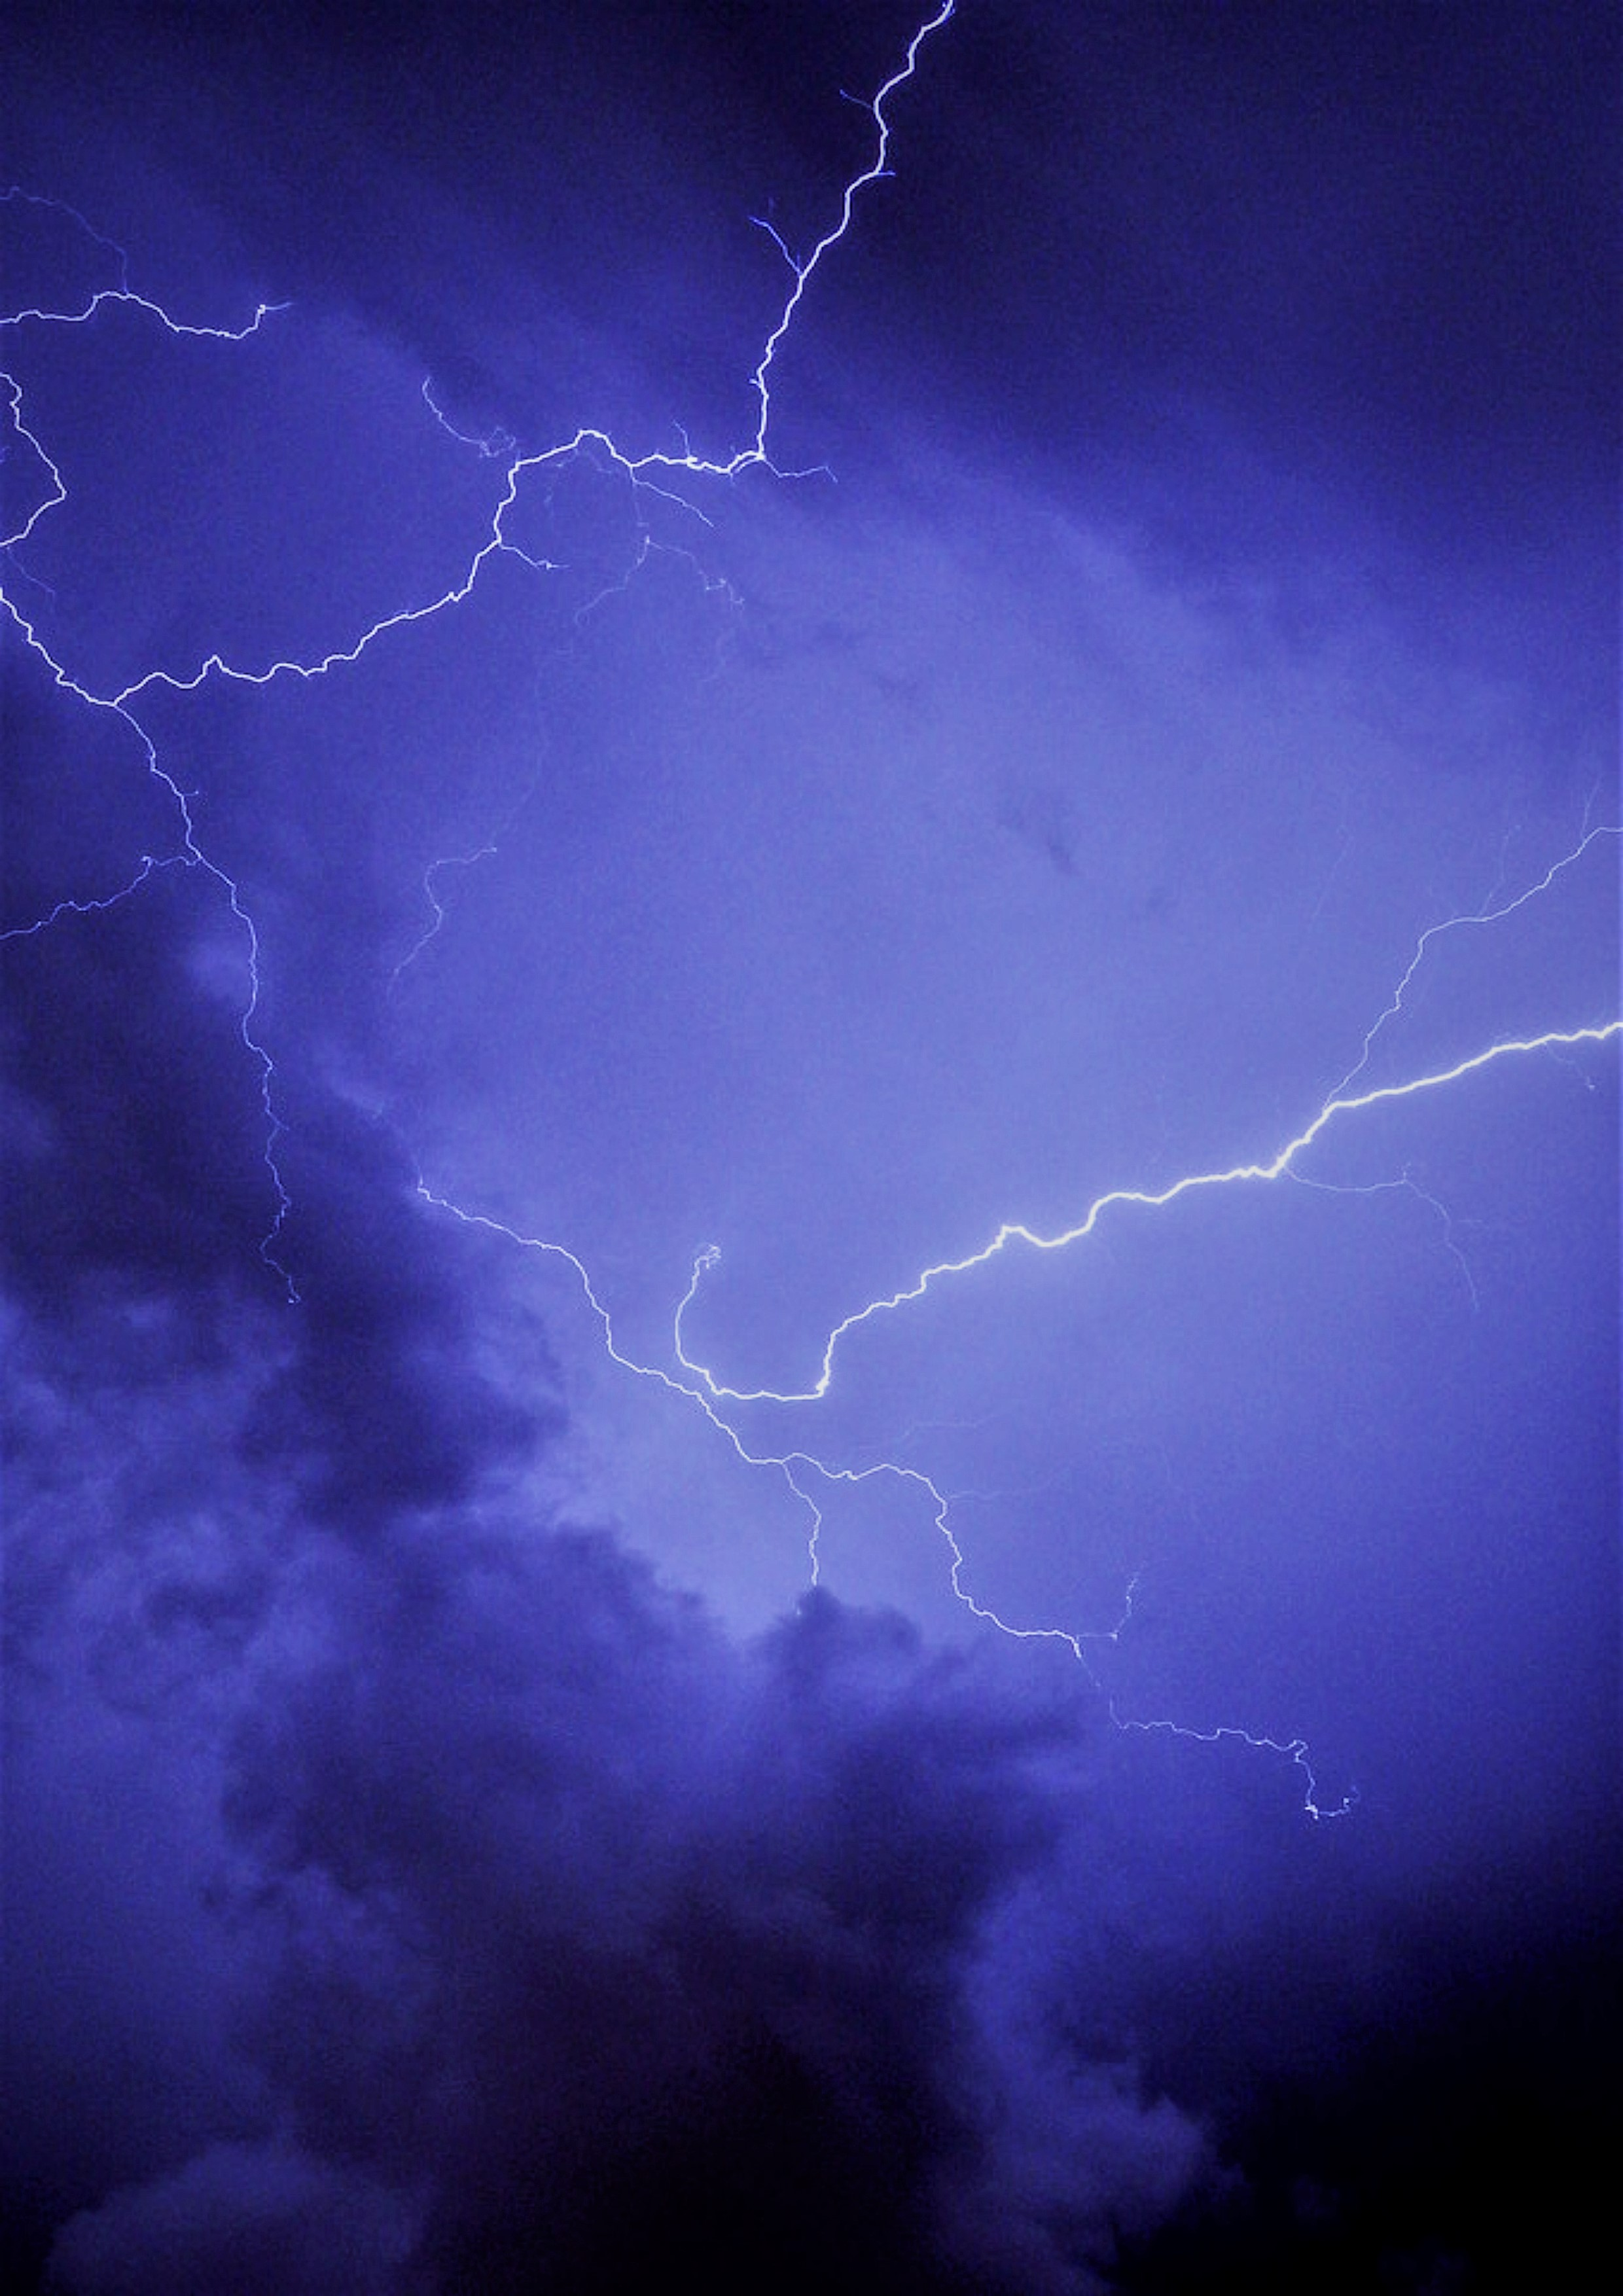
\includegraphics[width=\paperwidth]{Pictures/portada0.jpg}}; % Background image
\draw[anchor=north] (midpoint) node [fill=ocre!30!white,fill opacity=0.6,text opacity=1,inner sep=1cm]{\Huge\centering\bfseries\sffamily\parbox[c][][t]{\paperwidth}{\centering Teoría de Circuitos I\\[15pt] % Book title
{\Large Escuela Técnica Superior de Ingeniería y Diseño Industrial}\\[20pt] % Subtitle
{\huge 2022/23}}}; % Author name
\end{tikzpicture}};
\end{tikzpicture}
\vfill
\endgroup
	
% 	\begingroup
% 	\thispagestyle{empty}
% 	\AddToShipoutPicture*{\put(0,0){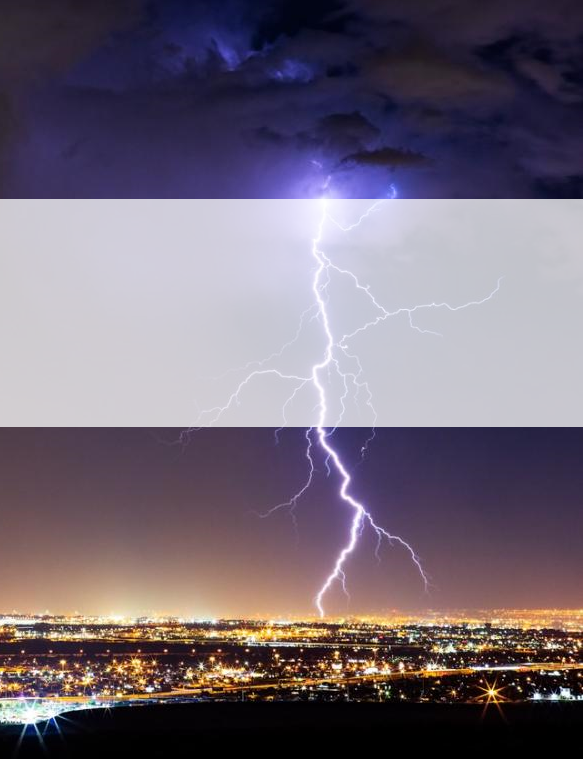
\includegraphics[scale=2.1]{Pictures/portada0.png}}} % Image background
% 	\centering
% 	\vspace*{5.2cm}
% 	\par\normalfont\fontsize{35}{35}\sffamily\selectfont
% 	\textbf{Teoría de circuitos}\\
% 	{\LARGE Curso: 2022/2023}\par % Book title
% 	\vspace*{1cm}
% 	{\huge Grado en Ingeniería Eléctrica}\par % Author name
% 	\endgroup
	
	%----------------------------------------------------------------------------------------
	%	COPYRIGHT PAGE
	%----------------------------------------------------------------------------------------
	
	\newpage
	~\vfill
	\thispagestyle{empty}
	
	\noindent \textsc{Universidad Politécnica de Madrid}\\
	
	\noindent \href{}\\ % URL
	
	\noindent \textsc{Apuntes de la asignatura \emph{Teoría de circuitos} realizados por Ana Fernández Guillamón y	Oscar Perpiñán Lamigueiro. Se trata de una asignatura común a todos los Grados impartidos en la Escuela Técnica Superior de Ingeniería y Diseño Industrial}\\ % License information
	
	%\noindent \textit{Versi\'{o}n: \printdate} % Printing/edition date
	
	%----------------------------------------------------------------------------------------
	%	TABLE OF CONTENTS
	%----------------------------------------------------------------------------------------
	
	\chapterimage{indice.jpg} % Table of contents heading image
	
	\pagestyle{empty} % No headers
	
	\tableofcontents % Print the table of contents itself
	
	%\cleardoublepage % Forces the first chapter to start on an odd page so it's on the right
	
	\pagestyle{fancy} % Print headers again
	
	%----------------------------------------------------------------------------------------
	%	CHAPTER 1
	%----------------------------------------------------------------------------------------
	
	\chapterimage{imagen_t1.jpg} % Chapter heading image
	\chapter{Fundamentos. Corriente continua}\label{chap.cc}
	
	\setcounter{page}{1}
	
	%Referencias: \cite{edminister1988circuitos,usaola2003circuitos}
	
	\section{Introducción}
	
	La electricidad constituye una forma de energía que está presente en casi todas las actividades del hombre de una sociedad desarrollada, ya que gran parte de los aparatos y máquinas que usamos funcionan con ella. Produce efectos luminosos, mecánicos, caloríficos, químicos, etc., y se debe a la separación o movimiento de los electrones que forman los átomos. Las primeras observaciones de la atracción eléctrica ocurrieron en la antigua Grecia, donde observaron que, al frotar ámbar, éste atraía pequeños objetos livianos (paja, plumas, tela...). De hecho, el concepto de fuerza eléctrica tuvo su origen en experimentos muy sencillos como la frotación de dos cuerpos entre sí, al ver que cuando se frota una varilla de vidrio o de ámbar con un trapo o piel, éstas son capaces de desplazar piezas muy ligeras. Así, apareció la propiedad llamada \textbf{carga eléctrica} que causa este comportamiento. Además, se observaron dos tipos de acciones, \textbf{atracción} y \textbf{repulsión}, asociadas, por tanto, a la existencia de dos tipos de cargas (positiva y negativa). Con esta premisa, en el siglo XVIII, Benjamin Franklin sugirió que todo objeto posee una cantidad ``normal'' de electricidad y, cuando dos objetos se frotan entre sí, parte de la electricidad se transfiere de un cuerpo al otro. 
	
	Además, la fuerza que actúa sobre dos cuerpos cargados es proporcional al producto de las cargas e inversamente proporcional al cuadrado de la distancia que las separa, teniendo en cuenta que cargas iguales se repelen y distintas se atraen (ley de Coulomb). El medio en que se encuentren las cargas va a influir en dicha fuerza, reflejado mediante la constante de proporcionalidad $k$ (constante de Coulomb):
	\begin{equation*}\label{eq.coulomb}
		\Vec{F}=k\cdot\dfrac{Q_1\cdot Q_2}{r^2}\cdot \Vec{u}
	\end{equation*}
	Esta fuerza es debida a la creación de un campo eléctrico $\Vec{E}$. Por tanto, se dice que en una región del espacio existe un \textbf{campo eléctrico} si al situar en ella cargas eléctricas, se originan fuerzas de tipo electrostático, regidas por la expresión anterior. De hecho, una carga crea un campo eléctrico en todo el espacio, y este campo ejerce una fuerza la otra carga. La fuerza es, por tanto, ejercida por el campo en la posición de la segunda carga, más que por la propia primera carga que se encuentra a cierta distancia:
	\begin{equation*}
		\Vec{E}=\dfrac{F}{q_0}
	\end{equation*}
	siendo $q_0$ una carga lo suficientemente pequeña para que su efecto sobre la distribución de carga sea despreciable. Entonces, el campo eléctrico es un vector que describe la condición en el espacio creada por un sistema de cargas puntuales, siendo, por tanto, una función vectorial de la posición. La fuerza ejercida sobre la carga testigo $q_0$ en cualquier punto está relacionada con el campo eléctrico por:
	\begin{equation*}
		\Vec{F}=q_0\cdot \Vec{E}.
	\end{equation*}
	
	
	\section{Conceptos fundamentales}
	
	\subsection{Circuito eléctrico} \label{sec.circuito_electrico}
	
	Un \textbf{circuito eléctrico} es un conjunto de componentes eléctricos combinados de tal forma que crean un camino cerrado por el que puede circular una corriente eléctrica. %
	%
	% \begin{theorem}[Circuito eléctrico]
		% Conjunto de elementos combinados de tal forma que existe la posibilidad de que se origine una corriente eléctrica.
		% \end{theorem}
	%
	Hay dos tipos de elementos que se pueden
	integrar en un circuito eléctrico: 
	\begin{itemize}
		\item \textbf{Elementos activos.} Dispositivos eléctricos que actúan como causas o factores motivantes para la circulación de la corriente eléctrica (generadores de tensión o corriente).
		\item \textbf{Elementos pasivos.} Componentes eléctricos que toman energía de los elementos activos para transformarla en otro tipo de energía, o acumularla en forma de campo magnético o eléctrico (receptores: resistencias, bobinas y condensadores). 
	\end{itemize}
	
	El \textbf{análisis} (o resolución) de un circuito eléctrico existente persigue determinar sus condiciones de funcionamiento, es decir, definir las ecuaciones correspondientes al circuito, así como obtener los valores de determinadas variables importantes a partir de dichas ecuaciones. Por contra, el \textbf{diseño} (o síntesis) de un circuito eléctrico tiene como objetivo definir el circuito eléctrico, es decir, determinar los componentes necesarios y su interconexión, para obtener unas condiciones de funcionamiento.
	
	Este curso está dedicado al análisis de circuitos eléctricos \textbf{lineales} de \textbf{parámetros concentrados}. 
	\begin{itemize}
		\item Al considerar que todos los circuitos eléctricos se comportan como sistemas lineales, se cumplen las dos condiciones mostradas a continuación:
		\begin{enumerate}
			\item $f(x + y) = f(x) + f(y)$: La respuesta $f$ a la suma de dos entradas $x$ e $y$ es igual a la suma de la respuesta individual a cada una de las entradas.
			\item $f(k \cdot x) = k \cdot f(x)$: La respuesta a una entrada que está multiplicada por un factor de escala $k$ es igual a multiplicar por este factor a la respuesta a la entrada.
		\end{enumerate}
		Al considerar el circuito como lineal, se simplifica su tratamiento de los circuitos, y \textbf{se puede aplicar técnicas de resolución de ecuaciones lineales}. Sin embargo, debe recordarse que la linealidad es una \textbf{aproximación de la realidad}, que no puede aplicarse de manera indiscriminada a cualquier componente y en cualquier condición. En particular, los \textbf{dispositivos electrónicos} como diodos o transistores tienen un \textbf{comportamiento} marcadamente \textbf{no lineal}, de forma que los circuitos que los contienen no pueden analizarse directamente con las técnicas que aquí se exponen sin realizar previamente aproximaciones de su funcionamiento.
		\item El análisis de circuitos no toma en consideración las propiedades espaciales de los circuitos ni de sus componentes, sino que los \textit{confina} a elementos puntuales con un modelo de \textbf{parámetros concentrados}. Sin embargo, los circuitos eléctricos reales ocupan espacio, las máquinas generadoras y los receptores tienen grandes dimensiones, y los cables conductores se extienden a lo largo de longitudes variopintas. Por ejemplo, un conductor real de 100~m se representa con este modelo de parámetros concentrados como un conductor ideal con una resistencia en su punto medio. Este tratamiento es una simplificación de las ecuaciones del electromagnetismo de Maxwell, y es aplicable únicamente cuando las dimensiones del circuito real son inferiores a la longitud de onda de la señal que circula por el circuito. Así, a la frecuencia de 50~Hz (habitual en sistemas eléctricos industriales), la longitud de onda de la señal es de 6000~km, mientras que a la frecuencia de 2.6~GHz (característica de la telefonía 4G), la longitud de onda se reduce a 11.5~cm.
	\end{itemize}
	
	\subsection{Variables}
	\subsubsection{Tensión eléctrica}
	El \textbf{potencial eléctrico} en un punto, $v(t)$,  es la energía potencial que tiene una carga unitaria en ese punto debida al campo eléctrico. Dado que la fuerza electrostática $\vec{F}$ (definida con la ecuación~\eqref{eq.coulomb}) es conservativa, la variación de la energía potencial $dV$ viene dada por:
	\begin{equation*}
		dV=-\Vec{F}\cdot d\vec{l}=-q_0\cdot \Vec{E}\cdot d\vec{l}
	\end{equation*}
	donde $d\vec{l}$ es el desplazamiento que experimenta la carga debido al campo eléctrico $\Vec{E}$. La \textbf{tensión} o \textbf{diferencia de potencial entre dos puntos}, $u_{AB}(t)$ (Figura~\ref{fig.tension_puntos}), es el trabajo realizado por el campo eléctrico al desplazar una carga unitaria entre esos puntos: 
	\begin{equation*}
		u_{AB}(t) = v_A(t) - v_B(t) = \frac{dW_{e}}{dq_0}.
	\end{equation*}
	\begin{figure}[htbp]
		\centering
		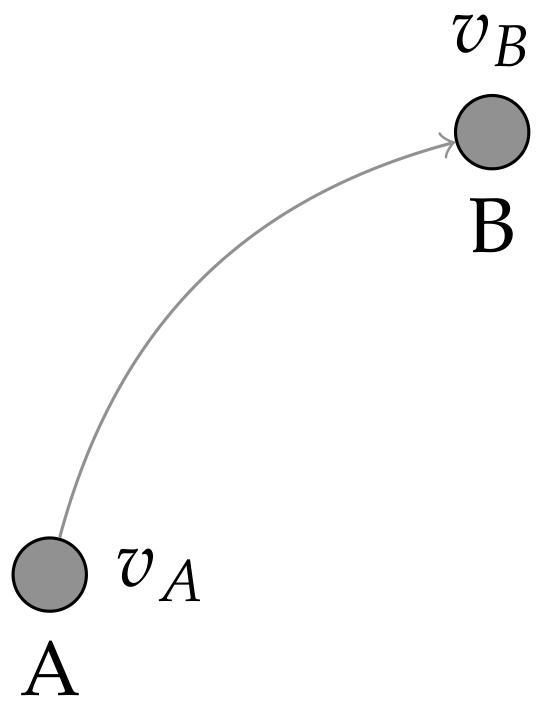
\includegraphics[width=0.2\linewidth]{Pictures/tension_puntos.PNG}
		\caption{Diferencia de potencial}
		\label{fig.tension_puntos}
	\end{figure}
	
	Puesto que el potencial eléctrico es el trabajo electrostático por unidad de carga, la unidad del SI para $v(t)$ y $u_{AB}(t)$ es el \textbf{voltio} [V]:
	\begin{equation*}
		1\;V=\dfrac{1\;J}{1\;C}.
	\end{equation*}
	\begin{remark}
		La unidad [V] se escribe en mayúsculas en honor a Alessandro Volta, físico y químico italiano del siglo XVIII famoso por la invención y desarrollo de la pila eléctrica en 1799.
	\end{remark}
	Además, el campo eléctrico también es conservativo, por lo que la diferencia de potencial entre A y B \textbf{no depende de la trayectoria} seguida para realizar el desplazamiento, sino únicamente del potencial existente en cada uno de los puntos (Figura~\ref{fig.diagrama_tension}). Sin embargo, y pese a que la trayectoria no es relevante, siempre hay que tener en cuenta el \textbf{sentido del desplazamiento} (Figura~\ref{fig.sentido_tension}). Así, si el movimiento se produce desde B hasta A.
	\begin{equation*}
		u_{BA}(t) = v_B(t) - v_A(t) = - u_{AB}(t). 
	\end{equation*}
	\begin{figure}[htbp]
		\centering
		\subfigure[Trayectoria]{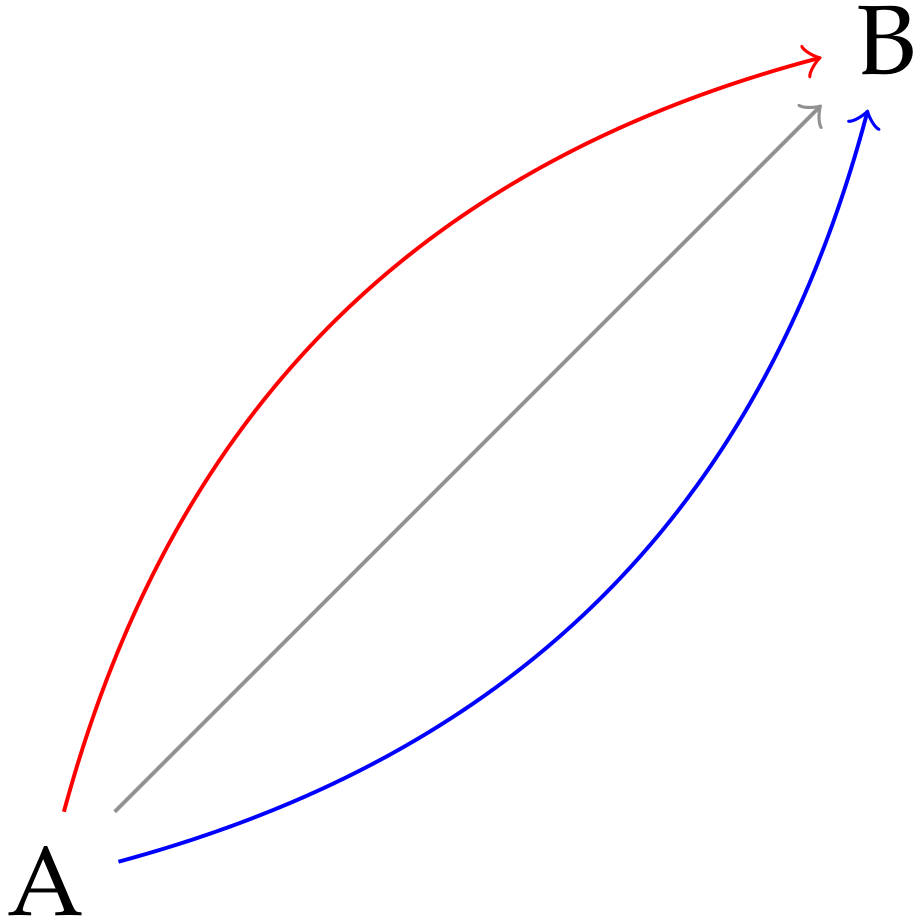
\includegraphics[width=0.25\linewidth]{Pictures/diagrama_tension.PNG}\label{fig.diagrama_tension}}\hfil
		\subfigure[Sentido]{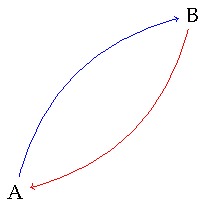
\includegraphics[width=0.25\linewidth]{Pictures/sentido_tension.pdf}\label{fig.sentido_tension}}
		\caption{Consideraciones sobre la diferencia de potencial}
	\end{figure}
	
	\subsubsection{Corriente eléctrica}
	La \textbf{intensidad de la corriente eléctrica}, $i(t)$, se define como la variación de la carga eléctrica $q(t)$ que atraviesa la sección transversal de un conductor por unidad de tiempo (Figura~\ref{fig.seccion_conductor}). 
	\begin{equation*}\label{eq.intensidad}
		i(t)=\dfrac{dq(t)}{dt}
	\end{equation*}
	\begin{figure}[htbp]
		\centering
		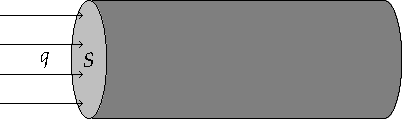
\includegraphics[width=0.45\linewidth]{Pictures/seccion_conductor.pdf}
		\caption{Corriente eléctrica}
		\label{fig.seccion_conductor}
	\end{figure}
	
	La corriente eléctrica se produce por el \textbf{movimiento de los electrones libres} que fluyen por el conductor, es decir, que el \textbf{sentido real} de la intensidad es del polo $-$ al polo $+$ del generador (a través del conductor). Sin embargo, por razones históricas, el \textbf{convenio} que se emplea es justo el opuesto, esto es, del polo $+$ al polo $-$. La unidad en el SI de la corriente es el \textbf{amperio} [A]: 
	\begin{equation*}
		1\,A =\dfrac{1\,C}{1\,s}.
	\end{equation*}
	\begin{remark}
		La unidad [A] se escribe en mayúsculas en honor a André-Marie Ampère, matemático y físico francés del siglo XVIII-XIX, que inventó el primer telégrafo eléctrico y formuló la teoría del electromagnetismo en 1827.
	\end{remark}
	
	Cabe resaltar que el amperio es una unidad muy grande, por lo que a menudo se utilizan submúltiplos (mA, $\mu$A...). En algunos casos puede hablarse también de la \textbf{densidad de corriente}, definida como el cociente entre la intensidad $i(t)$ y la sección transversal del conductor $S$:
	\begin{equation*}
		\delta =\dfrac{i(t)}{S}
	\end{equation*}
	La densidad de corriente se mide en el SI en [A/m$^2$], aunque en la industria suele venir determinada en [A/mm$^2$], al ser ésta una unidad más manejable.
	
	\subsubsection{Corriente continua y corriente alterna} \label{sec.cc-ca}
	Al estudiar la electricidad, es importante destacar que existen dos tipos de corriente: la corriente continua y la corriente alterna:
	\begin{itemize}
		\item \textbf{Corriente continua:} La corriente continua es aquella que siempre fluye en el mismo sentido (positivo o negativo). A su vez, puede ser:
		\begin{itemize}
			\item \textbf{Corriente continua constante:} Su valor instantáneo a lo largo del tiempo permanece inalterable ($\frac{di(t)}{dt} = 0$, Figura~\ref{fig.continua}). Suele estar suministrada por pilas, baterías, dinamos, fuentes de alimentación de corriente continua, etc. 
			\begin{figure}[htbp]
				\centering
				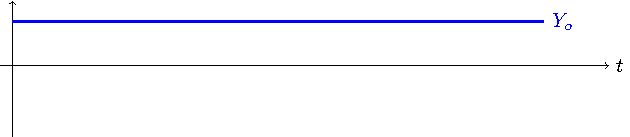
\includegraphics[width=0.75\linewidth]{Pictures/continua.pdf}
				\caption{Forma de onda de la corriente continua constante}
				\label{fig.continua}
			\end{figure}
			\item \textbf{Corriente continua variable:} Su valor instantáneo no es constante a lo largo del tiempo, aunque siempre es del mismo signo (negativo o positivo). 
		\end{itemize}
		\item \textbf{Corriente alterna:} Aquella corriente que cambia de sentido (de positivo a negativo, y viceversa) cada cierto tiempo ($\frac{di(t)}{dt} \neq 0$). Se subdivide de nuevo en varios tipos:
		\begin{itemize}
			\item \textbf{Corriente alterna sinusoidal:} Los valores absolutos instantáneos son sucesivamente proporcionales a los valores que toma el seno de 0$^\circ$ a 360$^\circ$ (Figura~\ref{fig.sin}).
			\begin{figure}[htbp]
				\centering
				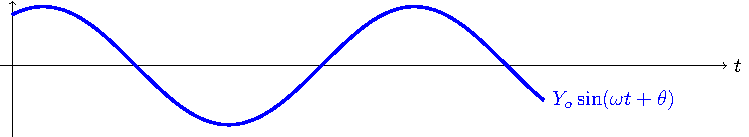
\includegraphics[width=0.75\linewidth]{Pictures/sin.pdf}
				\caption{Forma de onda de la corriente alterna senoidal}
				\label{fig.sin}
			\end{figure}
			\item \textbf{Corriente alterna periódica:} Tiene una forma de onda que se repite de manera periódica, cambiando de sentido, pero no es sucesivamente proporcional a los valores que toma el seno de 0$^\circ$ a 360$^\circ$.
			\item \textbf{Corriente alterna aperiódica:} Tiene una forma de onda que cambia de sentido pero sin seguir ningún periodo.
		\end{itemize}
	\end{itemize}
	Por comodidad, a la corriente continua constante se la conoce simplemente como \textit{corriente continua} (CC) y a la corriente alterna sinusoidal como \textit{corriente alterna} (CA).
	
	
	\subsubsection{Fuerza electromotriz (f.e.m.)}
	En todo circuito eléctrico es necesaria la existencia de al menos un elemento activo que suministre energía eléctrica, de manera que las cargas permanezcan en movimiento y, por tanto, exista corriente eléctrica. La causa capaz de mantener los electrones en movimiento en un circuito recibe el nombre de \textbf{fuerza electromotriz} (f.e.m.). Los dispositivos capaces de proporcionar esta diferencia de potencial estacionaria, permitiendo mantener una corriente eléctrica, son los \textbf{generadores} (baterías, pilas, dinamos, etc.), siendo la f.e.m. ($E$, $e(t)$ o $\epsilon$) la característica de éstos.  Por tanto, la fuerza electromotriz representa la energía que el generador cede a la unidad de carga eléctrica. Al tener la misma naturaleza que la tensión eléctrica, también se mide en voltios [V]. 
	
	\subsubsection{Potencia eléctrica}
	La \textbf{potencia eléctrica} es la variación del trabajo del campo eléctrico por unidad de tiempo:
	\begin{equation*}
		p(t)=\frac{dW_{e}}{dt} 
	\end{equation*}
	que puede relacionarse con las variables anteriores:
	\begin{equation*}\label{eq.pvi}
		p(t) = \frac{dW_e}{dq} \cdot \frac{dq(t)}{dt}= v(t)\cdot i(t)
	\end{equation*}
	
	La {unidad} de la potencia eléctrica en el SI es el \textbf{vatio} [W]: 
	\begin{equation*}
		1\;W = \dfrac{1\;J}{1\;s}= 1\;A\cdot 1\;V.
	\end{equation*}
	\begin{remark}
		La unidad [W] se escribe en mayúsculas en honor a James Watt, ingeniero mecánico, inventor y químico escocés de los siglos XVIII-XIX, por sus contribuciones al desarrollo de la máquina de vapor, fundamental en el desarrollo de la primera Revolución Industrial.
	\end{remark}
	
	Para determinar el \textbf{signo de la potencia eléctrica} (Figura~\ref{fig.signo_potencia}) hay que tener en consideración los signos de las variables de las que depende (tensión y corriente): 
	\begin{itemize}
		\item Cuando las flechas de ambas variables tienen el \textbf{mismo sentido}, la potencia eléctrica es \textbf{positiva} ($P>0$)
		\item Cuando las flechas tienen \textbf{sentidos opuestos}, la potencia eléctrica es \textbf{negativa} ($P<0$)
	\end{itemize}
	\begin{figure}[htbp]
		\centering
		\subfigure[$P>0$]{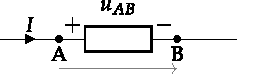
\includegraphics[width=0.3\linewidth]{Pictures/signo_potencia1.pdf}}\hfil
		\subfigure[$P<0$]{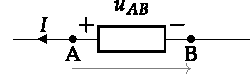
\includegraphics[width=0.3\linewidth]{Pictures/signo_potencia2.pdf}}
		\caption{Convenio de signos para la potencia}
		\label{fig.signo_potencia}
	\end{figure}
	En la práctica, no es conveniente trabajar con potencias negativas, por lo que es habitual interpretar este resultado como potencia absorbida y potencia generada/entregada (Figura~\ref{fig.receptor_generador}):
	\begin{itemize}
		\item Un circuito o elemento es un \textbf{receptor} (absorbe potencia) cuando la corriente \emph{entra} por el terminal de mayor potencial
		\item Un circuito o elemento es un \textbf{generador} (entrega potencia) cuando la corriente \emph{sale} por el terminal de mayor potencial
	\end{itemize}
	\begin{figure}[htbp]
		\centering
		\subfigure[Receptor]{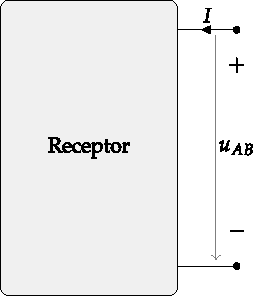
\includegraphics[width=0.25\linewidth]{Pictures/receptor_generador1.pdf}}\hfil
		\subfigure[Generador]{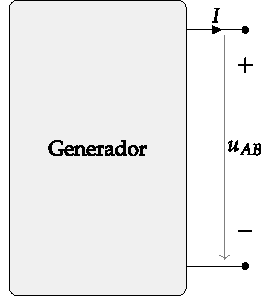
\includegraphics[width=0.25\linewidth]{Pictures/receptor_generador2.pdf}}
		\caption{Convenio de signos para la potencia}
		\label{fig.receptor_generador}
	\end{figure}
	
	\subsubsection{Energía y potencia}
	
	La \textbf{energía} $W$ es una magnitud física asociada con la capacidad que tienen los cuerpos para realizar un trabajo (emitir luz, generar calor, etc.). Puede manifestarse de distintas formas: gravitatoria, cinética, química, eléctrica, magnética, nuclear, radiante, etc., existiendo la posibilidad de transformar unos tipos de energía en otros, pero respetando siempre el principio de conservación de la energía. En el SI, la energía (del tipo que sea) se mide en julios [J]. El julio se define como el trabajo realizado por una fuerza $F$ de 1 Newton [N] cuando provoca un desplazamiento $d$ de 1 metro [m]. Por tanto, una forma de definir la energía es:
	\begin{equation*}
		W=F\cdot d 
	\end{equation*}
	\begin{remark}
		La unidad [J] se escribe en mayúsculas en honor a James Prescott Joule, físico e investigador inglés del siglo XIX, considerado como uno de los físicos más notables de su época. 
	\end{remark}
	
	Dado que la potencia $P$ se define como la cantidad de trabajo realizado (es decir, la energía $W$) por unidad de tiempo $t$ ($P=\frac{W}{t}$), también se puede definir la energía como:
	\begin{equation*}\label{eq.Ept}
		W=P\cdot t.
	\end{equation*}
	Por tanto, otra unidad muy utilizada para medir energía es el vatio-hora [Wh], aunque ésta \textbf{\emph{no}} es la aceptada en el SI. Esta unidad representa el trabajo realizado por una máquina de potencia 1 W durante un tiempo de 1 hora. El Wh se utiliza comúnmente para medir la \textbf{energía eléctrica}. 
	
	\vspace{4mm}
	\begin{example}
		\textbf{¿Cuál es la equivalencia entre un kWh y un J?}\\
		1 kWh = 1 kW $\cdot$ 1 h = 1000 W $\cdot$ 3600 s = 3.6 MJ 
	\end{example}
	
	\section{Elementos de los circuitos}
	Como ya se mencionó en la Sección~\ref{sec.circuito_electrico}, en un circuito eléctrico existen dos tipos de elementos: los elementos pasivos y los activos.
	
	\subsection{Elementos activos}\label{sec.elementos_activos}
	
	\subsubsection{Generadores de tensión}
	Un \textbf{generador de tensión} es un dispositivo físico, caracterizado por una fuerza electromotriz $\epsilon$ que proporciona una diferencia de potencial $U$ entre sus bornes de salida. Por tanto, \textbf{impone la tensión} a su salida, mientras que \emph{la corriente depende del circuito} (Figura~\ref{fig.fuentetension}).
	\begin{itemize}
		\item Un \textbf{generador ideal} es aquel que \textbf{no tiene pérdidas}, de tal forma que la diferencia de potencial entre sus bornes toma siempre el mismo valor que su f.e.m. ($u_{AB}=\epsilon_g$). Además, se dice que un generador de tensión ideal es \textbf{dominante} sobre todo lo que está conectado en paralelo con él, ya que impone entre sus terminales la tensión que lo caracteriza. Así, a efectos de cálculo, puede prescindirse de las ramas que no interese estudiar.
		\item Un \textbf{generador real} es aquel que \textbf{tiene pérdidas}, caracterizadas mediante una resistencia interna, en \textbf{serie}, $R_{\epsilon_g}$. Al circular una corriente por dicha resistencia, se consume en ella una potencia que no puede ser entregada por el generador. Las pérdidas internas son la causa de que la diferencia de potencial entre sus bornes sea inferior a la f.e.m. ($u_{AB}<\epsilon_g$). Con esto, la potencia generada será $P_g=\epsilon_g\cdot I$, la potencia disipada en la resistencia interna $P_p=R_{\epsilon_g}\cdot I^2$ y la potencia útil $P_u=U_{AB}\cdot I$ y, dado que tiene que cumplirse el principio de conservación de la energía:
		\begin{equation}
			P_g=P_u+P_p\rightarrow \boxed{ \epsilon_g=U_{AB}+ R_{\epsilon_g}\cdot I}
		\end{equation}
	\end{itemize}
	\begin{figure}[htbp]
		\centering
		\subfigure[Ideal]{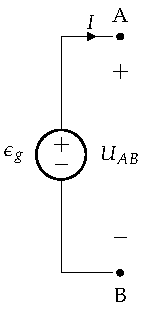
\includegraphics[height=3.5cm]{Pictures/FuenteTensionIdealDC.pdf}}\hfil
		\subfigure[Real]{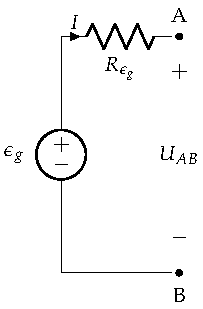
\includegraphics[height=3.5cm]{Pictures/FuenteTensionRealDC.pdf}}
		\caption{Generador de tensión}
		\label{fig.fuentetension}
	\end{figure}
	
	\subsubsection{Generadores de corriente}
	Un \textbf{generador de corriente} es un dispositivo físico, caracterizado por una intensidad $I_g$ que proporciona una corriente $I$ entre sus bornes de salida. Por tanto, \textbf{impone la corriente} a su salida, mientras que \emph{la tensión depende del circuito} (Figura~\ref{fig.fuentecorriente}).
	\begin{itemize}
		\item Un \textbf{generador ideal} es aquel que \textbf{no tiene pérdidas}, de tal forma que la corriente $I$ a su salida toma siempre el mismo valor que $I_g$ ($I=I_g$). Un generador de intensidad ideal es \textbf{dominante} sobre todo lo que está conectado en serie con él ya que impone en esa rama la corriente que lo caracteriza. A efectos de cálculo, puede prescindirse de los elementos en serie que no interese estudiar. 
		\item Un \textbf{generador real} es aquel que \textbf{tiene pérdidas}, caracterizadas mediante una resistencia interna, en \textbf{paralelo}, $R_{I_g}$. Al producirse una derivación de corriente por esa resistencia, circular una corriente por dicha resistencia, se consume en ella una potencia que no puede ser entregada por el generador. Las pérdidas internas son la causa de que la corriente suministrada sea menor a la que caracteriza al generador ($I<I_g$). Con esto, la potencia generada será $P_g=U_{AB}\cdot I_g$, la potencia disipada en la resistencia interna $P_p=\frac{U_{AB}^2}{R_{I_g}}$ y la potencia útil $P_u=U_{AB}\cdot I$ y, dado que tiene que cumplirse el principio de conservación de la energía:
		\begin{equation}
			P_g=P_u+P_p\rightarrow \boxed{I_g=I+ \dfrac{U_{AB}}{R_{I_g}}}
		\end{equation}
	\end{itemize}
	\begin{figure}[htbp]
		\centering
		\subfigure[Ideal]{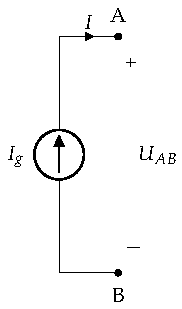
\includegraphics[height=3.5cm]{Pictures/FuenteCorrienteIdeal.pdf}}\hfil
		\subfigure[Real]{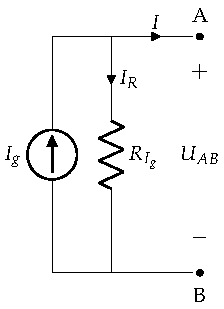
\includegraphics[height=3.5cm]{Pictures/FuenteCorrienteRealDC.pdf}}
		\caption{Generador de corriente}
		\label{fig.fuentecorriente}
	\end{figure}
	
	\subsubsection{Dualidad de generadores}\label{sec.dualidad}
	
	En la Sección~\ref{sec.elementos_activos} se presentaron las ecuaciones de los generadores de tensión y corriente, tanto del modelo ideal como del real. Además, se dice que dos fuentes son equivalentes cuando suministran el \textbf{mismo valor de tensión y corriente} a un circuito externo, para cualquier circuito. Esta equivalencia solo puede darse entre \textbf{fuentes reales}.
	
	\begin{figure}[htbp]
		\centering
		\subfigure[Fuente real de tensión]{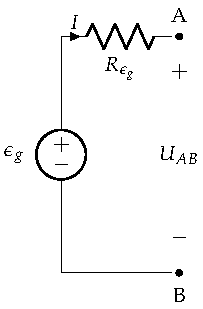
\includegraphics[height=4.9cm]{Pictures/FuenteTensionRealDC.pdf}}\hfil
		\subfigure[Fuente real de corriente]{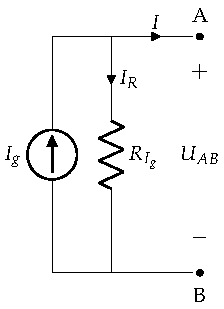
\includegraphics[height=4.9cm]{Pictures/FuenteCorrienteRealDC.pdf}}
		\caption{Equivalencia de generadores}
		\label{fig.equivalencia_generadores}
	\end{figure}
	
	Considérense las fuentes de tensión y corriente, reales, mostradas en la Figura~\ref{fig.equivalencia_generadores}
	La salida de la fuente de tensión es:
	\begin{equation*}
		U_{AB} = \epsilon_g - R_{\epsilon_g} \cdot I
	\end{equation*}
	y la de la fuente de corriente:
	\begin{equation*}
		I = I_g - \frac{U_{AB}}{R_{I_g}} \rightarrow U_{AB} = R_{I_g} \cdot I_g - R_{I_g} \cdot I
	\end{equation*} 
	Por tanto, las fuentes son equivalentes cuando las ecuaciones coinciden para cualquier combinación de $(U_{AB}, I)$, es decir, si $R_g = R_{\epsilon_g} = R_{I_g}$:
	\begin{equation}\label{eq.equivalencia_fuentes}
		\boxed{\epsilon_g = R_{\epsilon_g} \cdot I_g \Leftrightarrow {I_g = \frac{\epsilon_g}{R_g}}}  
	\end{equation}
	
	\begin{remark}
	    Nótese que el polo $+$ de la fuente de tensión queda en la misma posición que la flecha de la fuente de corriente
	\end{remark}
	
	\begin{example}
	    \textbf{Convertir en fuente de intensidad o de tensión, según corresponda, las siguientes fuentes. }
	    
	    EJERCICIO 1.7 DE PROBLEMAS BT1 CURSO 21-22
	\end{example}
	
	\subsubsection{Generadores dependientes o generadores controlados}
	Pese a no ser estrictamente elementos activos, se comportan como tales. Este tipo de generadores no tienen valores de $\epsilon$ o $i_g$ fijos, sino que dependen de la tensión o corriente en otros puntos de la red. Así, aparecen fundamentalmente cuatro tipos de generadores dependientes, dependiendo de que cada generador suministre una tensión o una corriente y según sea la variable de control una tensión o una corriente. Estos generadores suelen representarse mediante un rombo:
	\begin{itemize}
		\item \textbf{Generador de tensión controlado por tensión} (Figura~\ref{fig.tension-tension}): su tensión depende de la tensión entre otros puntos del circuito, siendo el parámetro $\alpha$ adimensional [--]
		\item \textbf{Generador de tensión controlado por corriente} (Figura~\ref{fig.tension-corriente}): su tensión depende de alguna corriente del circuito, teniendo el parámetro $\beta$ unidades de resistencia [$\Omega$]
		\item \textbf{Generador de corriente controlado por tensión} (Figura~\ref{fig.corriente-tension}): su intensidad depende de la tensión entre dos puntos del circuito, teniendo el parámetro $\gamma$ unidades de conductancia [S]
		\item \textbf{Generador de corriente controlado por corriente} (Figura~\ref{fig.corriente-corriente}): su intensidad es función de la corriente en otra parte del circuito, siendo el parámetro $\sigma$ adimensional [--]
	\end{itemize}
	\begin{figure}[htbp]
		\centering
		\subfigure[Tensión--Tensión]{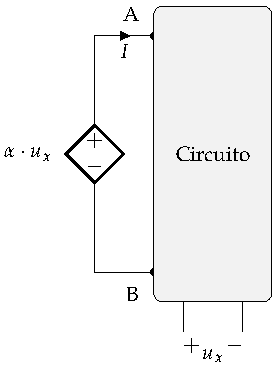
\includegraphics[height=4cm]{Pictures/FuenteTensionDependienteTension.pdf}\label{fig.tension-tension}}\hfill
		\subfigure[Tensión--Corriente]{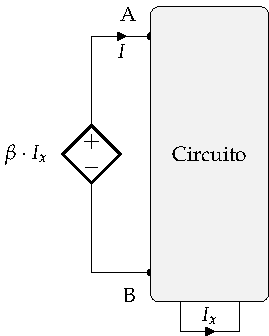
\includegraphics[height=4cm]{Pictures/FuenteTensionDependienteCorriente.pdf}\label{fig.tension-corriente}}\hfill
		\subfigure[Corriente--Tensión]{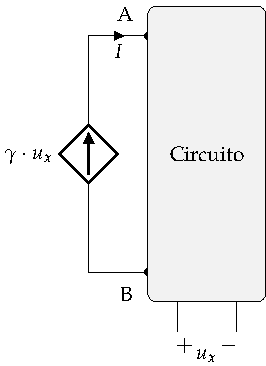
\includegraphics[height=4cm]{Pictures/FuenteCorrienteDependienteTension.pdf}\label{fig.corriente-tension}}\hfill
		\subfigure[Corriente--Corriente]{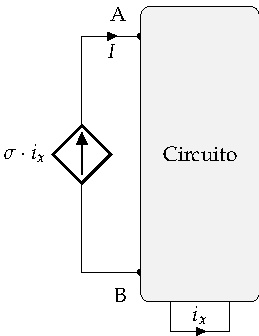
\includegraphics[height=4cm]{Pictures/FuenteCorrienteDependienteCorriente.pdf}\label{fig.corriente-corriente}}
		\caption{Fuentes dependientes}
		\label{fig.fuentes_dependientes}
	\end{figure}
	
	\begin{remark}
		Si en un circuito \textbf{solo} existen generadores dependientes, el circuito \textbf{no estaría excitado}.
	\end{remark} 
	
	
	
	
	
	\subsection{Elementos pasivos}\label{sec.elementos_pasivos}
	
	% Los receptores son todos aquellos dispositivos capaces de transformar la energía eléctrica en otra forma de energía (por ejemplo, un motor transforma la energía eléctrica en energía mecánica). Se caracterizan por su fuerza contraelectromotriz
	% (f.c.e.m., $E'$ o $e'(t)$), que es la energía por unidad de carga que transforman
	% en otro tipo de energía (siempre que ésta no sea calor). Por su definición, la unidad en el SI es también el \textbf{voltio} [V].
	
	En general, en teoría de circuitos se emplean tres tipos de elementos pasivos: resistencias, bobinas y condensadores. En general, se dice que un receptor es cualquier dispositivo capaz de transformar la energía eléctrica en otra forma de energía (que no sea solo calor); así, un ejemplo de receptor es un motor eléctrico (transforma parte de la energía eléctrica en mecánica).  
	
	\subsubsection{Resistencia}
	En el siglo XIX, Georg Simon Ohm descubrió la ley que lleva su nombre (\textbf{ley de Ohm}). Dicha ley obtiene que, \textit{a temperatura constante}, la relación existente entre la diferencia de potencial entre los bornes de un conductor y la intensidad de corriente que circula por él es una constante, denominada \textbf{resistencia eléctrica}:
	\begin{equation*}
		\boxed{u(t)=R\cdot i(t)}
	\end{equation*}
	Por tanto, la resistencia eléctrica representa la mayor o menor dificultad que ofrecen los diferentes materiales para ser recorridos por una corriente eléctrica. Su valor se mide en ohmios [$\Omega$]. El criterio de signos utilizado considerar que la tensión es positiva en el terminal por el que entra la corriente, esto es, las flechas de tensión y corriente tienen el mismo sentido (Figura~\ref{fig.resistencia}).
	\begin{figure}[htbp]
		\centering
		\subfigure[Referencia mediante signo]{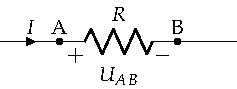
\includegraphics{Pictures/Resistencia.pdf}}\hfil
		\subfigure[Referencia mediante flecha]{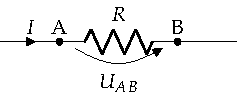
\includegraphics{Pictures/Resistencia_Flecha.pdf}}
		\caption{Criterio de signos en una resistencia}
		\label{fig.resistencia}
	\end{figure}
	
	La magnitud que determina si un material es mejor o peor conductor se denomina \textbf{resistividad} ($\rho$), medida en [$\Omega\cdot$m] en el SI, aunque en las aplicaciones prácticas se suele utilizar el [$\Omega\cdot$m$^2/m$]. La resistividad de un material permanece constante si no varía la temperatura (suele expresarse a 20$^\circ$C). Para conductores homogéneos, de sección constante y pequeña comparada con su longitud, la resistencia $R$ que ofrece al paso de la corriente se puede determinar a partir de: 
	\begin{equation*}\label{eq.resistencia_rho}
		R=\rho\cdot \dfrac{l}{S}
	\end{equation*}
	siendo $l$ la longitud del conductor y $S$ el área de la sección transversal del mismo. Cabe destacar, por su importancia en la industria, la resistividad del cobre ($\rho_{Cu}=1/56\;\Omega \cdot$m/mm$^2$) y la del aluminio ($\rho_{Al}=1/35\;\Omega \cdot$m/mm$^2$).
	
	\vspace{4mm}
	\begin{example}
		\textbf{Calcular la resistencia de un conductor de cobre tiene una longitud $l=10$~m y una sección $S=2$~mm$^2$.}\\
		Aplicando la anterior: 
		\begin{equation*}
			R=\rho\cdot \dfrac{l}{S}=(1/56)\cdot \dfrac{10}{2}=0.089\;\Omega
		\end{equation*}
	\end{example}
	
	Para temperaturas distintas de 20$^\circ$C, siempre que la temperatura final $T_f$ esté en torno a los 250$^\circ$, la resistividad y, por tanto, la resistencia pueden determinarse a partir de las siguientes expresiones:
	\begin{equation*}
		\rho_f=\rho_{20}\cdot (1+\alpha\cdot (T_f-20)); \qquad
		R_f=R_{20}\cdot (1+\alpha\cdot (T_f-20))
	\end{equation*}
	donde $\rho_f$ y $R_f$ son la resistividad y la resistencia a la temperatura $T_f$ (respectivamente), $\rho_{20}$ y $R_{20}$ son la resistividad y la resistencia a 20$^\circ$C (respectivamente) y $\alpha$ es el coeficiente de temperatura. 
	
	La inversa de la resistencia se denomina \textbf{conductancia}, $G$, y se mide en el SI en \textbf{Siemens} [S]. Al ser lo opuesto de la resistencia, representa la facilidad de los conductores al paso de la corriente eléctrica:
	\begin{equation}
		\boxed{G=\dfrac{1}{R}}
	\end{equation}
	\begin{remark}
		La unidad [S] se escribe en mayúsculas en honor a Ernst Werner M. von Siemens, inventor alemán del siglo XIX, pionero de la electrotecnia y fundador de la actual empresa Siemens.
	\end{remark}
	Asimismo, a la inversa de la resistividad se le denomina \textbf{conductividad} ($\gamma$), definida como la facilidad que ofrecen los materiales al paso de la corriente eléctrica, por unidad de longitud y sección:
	\begin{equation*}
		\gamma=\dfrac{1}{\rho}
	\end{equation*}
	
	El desplazamiento de cargas a través de los conductores produce interacciones y choques entre ellas que, a su vez, dan
	origen a un calentamiento del conductor. El físico británico James Prescott Joule, en 1841, fue quién cuantificó el valor del calor que se produce en un conductor por el paso de la corriente y enunció la ley que lleva su nombre (\textbf{ley de Joule}): toda la energía que absorbe un conductor homogéneo por el que circula una corriente eléctrica y en el que no existen f.e.m., se transforma íntegramente en calor. Por tanto, la energía ``perdida'' en forma de calor, considerando la expresiones~\eqref{eq.pvi}, \eqref{eq.Ept} y la ley de Ohm:
	\begin{equation*}
		W=P\cdot t=U\cdot I\cdot t=R\cdot I^2\cdot t
	\end{equation*}
	cuyo resultado viene expresado en [J]. Sin embargo, una unidad muy utilizada para medir el calor es la \textbf{caloría} [cal], cuya equivalencia con el [J] es:
	\begin{equation*}
		1\;J=0.24\;cal
	\end{equation*}
	En general, se dirá que una resistencia disipa energía eléctrica produciendo calor, siendo la potencia disipada: 
	\begin{equation*}
		p(t)=R\cdot i^{2}(t)
	\end{equation*}
	
	El concepto de resistencia se utiliza también para definir dos términos muy comunes en teoría de circuitos:
	\begin{itemize}
		\item \textbf{Cortocircuito:} Conductor ideal que se une entre dos puntos, haciendo de este modo que su resistencia es $R=0\;\Omega$. El cortocircuito puede llevar cualquier corriente, cuyo valor depende del resto del circuito, pero la tensión entre sus terminales (por la ley de Ohm) es de $v(t)=0$~V (Figura~\ref{fig.cortocircuito}). 
		\item \textbf{Circuito abierto:} Representa una ruptura del circuito en ese punto, por lo que no puede circular corriente ($i(t)=0$). Se puede considerar como un circuito con resistencia infinita ($R\rightarrow\infty$) y que puede tener cualquier tensión, que depende del resto de la red (Figura~\ref{fig.c_abierto}).
	\end{itemize}
	\begin{figure}[htbp]
		\centering
		\subfigure[Cortocircuito]{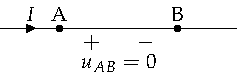
\includegraphics[width=0.2\linewidth]{Pictures/cortocircuito.pdf}\label{fig.cortocircuito}}\hfil
		\subfigure[Circuito abierto]{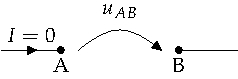
\includegraphics[width=0.2\linewidth]{Pictures/CircuitoAbierto.pdf}\label{fig.c_abierto}}
		\caption{Cortocircuito y circuito abierto}
		
	\end{figure}
	
	\subsubsection{Bobina}\label{sec.bobina}
	
	Una \textbf{bobina} es un conductor arrollado, con $N$ vueltas, alrededor de un núcleo (generalmente, de material ferromagnético). La tensión en bornes de la bobina es directamente proporcional a la variación de la corriente respecto al tiempo, con un factor de proporcionalidad $L$ conocido como es la \textbf{inductancia} o coeficiente de autoinducción, medido en \textbf{henrios} [H] (Figura~\ref{fig.bobina}):
	\begin{equation}\label{eq.u_L}
		\boxed{u(t)=L\cdot\frac{di(t)}{dt}}\,
	\end{equation}
	por lo que, en circuitos de corriente continua, una bobina se comporta como un \textbf{cortocircuito}:
	\begin{equation*}
		\dfrac{di(t)}{dt} = 0 \rightarrow u = 0
	\end{equation*}
	\begin{remark}
		La unidad [H] se escribe en mayúsculas en honor a Joseph Henry, físico estadounidense del siglo XIX conocido por su trabajo acerca del electromagnetismo, electroimanes y relés.
	\end{remark}
	\begin{figure}[htbp]
		\centering
		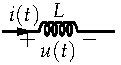
\includegraphics[width=0.15\linewidth]{Pictures/Bobina.pdf}
		\caption{Tensión y corriente en una bobina}
		\label{fig.bobina}
	\end{figure}
	
	La relación inversa de la expresión~\eqref{eq.u_L} se puede obtener por integración entre un tiempo inicial $t_iu$ y un tiempo final $t_f$, resultando:
	\begin{equation*}
		\int_{t_i}^{t_f} \dfrac{di(t)}{dt}dt=\dfrac{1}{L}\int_{t_i}^{t_f}u(t)\cdot dt \rightarrow i(t_f)-i(t_i)=\dfrac{1}{L}\cdot\int_{t_i}^{t_f} u(t)\cdot dt\,
	\end{equation*}
	\begin{equation}
		\boxed{i(t_f)=i(t_i)+\dfrac{1}{L}\cdot\int_{t_i}^{t_f} u(t)\cdot dt}
	\end{equation}
	Se observa que la bobina tiene un efecto de ``memoria'', ya que la corriente en un tiempo $t_f$ no depende solamente de la entrada $i(t)$ en ese momento, sino también del valor inicial de la entrada.
	
	Para entender el concepto de inductancia, es necesario recordar algunos principios del electromagnetismo. 
	\begin{itemize}
		\item \textbf{Ley de Ampère.} Es la ley fundamental que relaciona corrientes eléctricas y campos magnéticos. Su versión más simple dice que el producto de $N$ veces una corriente $i$ da lugar a una intensidad de campo magnético $H$ proporcional a la longitud magnética media de las líneas de dicho campo $l$:
		\begin{equation*}
			\label{eq.ampere_mod}
			H\cdot l=N\cdot i
		\end{equation*}
		\item \textbf{Densidad de flujo magnético.} La intensidad de campo $H$ origina, allá donde exista, una densidad de flujo $B$, cuyo valor es:
		\begin{equation*}\label{eq.B}
			B=\mu\cdot H,
		\end{equation*}
		siendo $\mu$ la permeabilidad del material. 
		\item \textbf{Flujo magnético.} Un campo magnético $B$ (constante en magnitud y dirección) que atraviesa un área $S$, formando un ángulo $\theta$ con ésta, crea un flujo magnético que se puede calcular como: 
		\begin{equation*}\label{eq.flujo1}
			\phi=B\cdot S\cdot \cos (\theta)
		\end{equation*}
		\item \textbf{Ley de Lenz-Faraday.} Un flujo magnético variable en el tiempo induce una fuerza electro-motriz (fem, $e$) que es igual en magnitud a la variación por unidad de tiempo del flujo inducido en el circuito. Esta fem inducida tiene un sentido tal que sus efectos tienden a oponerse a las causas que lo producen, por lo que: 
		\begin{equation*}\label{eq.lenz-faraday}
			e=-\dfrac{d\phi(t)}{dt}.
		\end{equation*}
	\end{itemize}
	A partir de esto, y con la ecuación~\eqref{eq.u_L}, es sencillo concluir que, cuando un circuito está formado únicamente por una bobina alimentada con una intensidad variable (es decir, corriente alterna) el flujo magnético también cambia y, por tanto, se induce una $fem$:
	\begin{equation*}
		e=\dfrac{d\phi(t)}{dt}=L\cdot \dfrac{di(t)}{dt} 
	\end{equation*}
	es decir, la $fem$ inducida es proporcional a la variación con el tiempo de la intensidad de corriente. Considerando esta expresión y despejando el valor de $L$, se tiene que: 
	\begin{equation*}
		L= \dfrac{d\phi(t)}{\cancel{dt}}\cdot\dfrac{\cancel{dt}}{di(t)}=\dfrac{d\phi(t)}{di(t)}
	\end{equation*}
	por lo que la inductancia $L$ expresa la relación entre el cambio de flujo y el cambio de corriente. 
	
	Además, para establecer un flujo en una bobina, es necesario una energía de entrada, que queda almacenada después en forma de \textbf{campo magnético}. La potencia ``absorbida'' por la bobina será:
	\begin{equation*}
		p(t)=u(t)\cdot i(t)=L\cdot i(t)\cdot\dfrac{di(t)}{dt}
	\end{equation*}
	y la energía almacenada $w(t)$ en un periodo de tiempo entre $t_i$ y $t_f$ valdrá:
	\begin{equation*}
		w(t)=\int_{t_i}^{t_f}v(t)\cdot i(t)\cdot dt=\int_{t_i}^{t_f}L\cdot\dfrac{di(t)}{dt}\cdot i(t)\cdot dt=\dfrac{1}{2}\cdot L\cdot [i(t_f)-i(t_i)]^2
	\end{equation*}
	\begin{equation}
		\boxed{w(t)=\dfrac{1}{2}\cdot L\cdot [i(t_f)-i(t_i)]^2}
	\end{equation}
	
	\subsubsection{Condensador}\label{sec.condensador}
	
	Un sistema de dos placas metálicas separadas por una capa dieléctrica constituye un \textbf{condensador}. Al aplicar tensión, produciendo una \textbf{separación de cargas opuestas} que se \textbf{acumulan} en cada placa (una de las placas queda con la carga $+Q$ y el otro con $-Q$). Del mismo modo que un elemento resistivo se distingue por el valor de su resistencia $R$, y una bobina por el valor de su inductancia $L$, un condensador se caracteriza por su \textbf{capacidad} $C$, que es la aptitud que tiene para acumular carga eléctrica. Así, la capacidad es la relación entre la carga $q(t)$ acumulada y la diferencia de potencial aplicada entre ellas $u(t)$, siendo:
	\begin{equation}\label{eq.cqu}
		\boxed{C=\dfrac{q(t)}{u(t)}}
	\end{equation}
	La unidad en el SI de la capacidad es el faradio [F]. Se trata de una unidad tremendamente grande, por lo que en la práctica se utilizan submúltiplos (mF, $\mu$F, pF...). 
	\begin{remark}
		La unidad [F] se escribe en mayúsculas en honor a Michael Faraday, científico británico de los siglos XVIII-XIX que estudió el electromagnetismo y la electroquímica. 
	\end{remark}
	
	Durante la carga del condensador, se produce una corriente eléctrica entre las dos placas (Figura~\ref{fig.condensador}): 
	\begin{equation*}\label{eq.icu}
		i(t)=\dfrac{dq(t)}{dt}\stackrel{\eqref{eq.cqu}}{=}\dfrac{d(C\cdot u(t))}{dt}=C\cdot \dfrac{du(t)}{dt}
	\end{equation*}
	por lo que, en circuitos de corriente continua, un condensador se comporta como un \textbf{circuito abierto}.
	\begin{equation*}
		\frac{du(t)}{dt} = 0 \rightarrow i = 0
	\end{equation*}
	\begin{figure}[htbp]
		\centering
		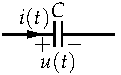
\includegraphics[width=0.15\linewidth]{Pictures/Condensador.pdf}
		\caption{Tensión y corriente en un condensador}
		\label{fig.condensador}
	\end{figure}
	
	La relación inversa de la expresión~\eqref{eq.icu} se puede obtener por integración entre un tiempo inicial $t_iu$ y un tiempo final $t_f$, resultando:
	\begin{equation*}
		\int_{t_i}^{t_f} \dfrac{du(t)}{dt}dt=\dfrac{1}{C}\int_{t_i}^{t_f}i(t)\cdot dt \rightarrow u(t_f)-u(t_i)=\dfrac{1}{C}\cdot\int_{t_i}^{t_f} i(t)\cdot dt
	\end{equation*}
	\begin{equation}\label{eq.u_C}
		\boxed{u(t_f)=u(t_i)+\dfrac{1}{C}\cdot\int_{t_i}^{t_f} i(t)\cdot dt}
	\end{equation}
	Se observa que el condensador también tiene un efecto de ``memoria'', ya que la tensión en un tiempo $t_f$ no depende solamente de la entrada $u(t)$ en ese momento, sino también del valor inicial.
	
	Al aplicar tensión a un condensador se produce una separación de cargas entre ambas placas, lo que produce un \textbf{campo eléctrico}, quedando almacenada una energía de este tipo. La potencia ``absorbida'' por el condensador será:
	\begin{equation*}
		p(t)=u(t)\cdot i(t)=C\cdot u(t)\cdot\dfrac{du(t)}{dt}
	\end{equation*}
	y la energía almacenada $w(t)$ en un periodo de tiempo entre $t_i$ y $t_f$ valdrá:
	\begin{equation*}
		w(t)=\int_{t_i}^{t_f}v(t)\cdot i(t)\cdot dt=\int_{t_i}^{t_f}C\cdot\dfrac{du(t)}{dt}\cdot u(t)\cdot dt=\dfrac{1}{2}\cdot C\cdot [u(t_f)-u(t_i)]^2
	\end{equation*}
	\begin{equation}
		\boxed{w(t)=\dfrac{1}{2}\cdot C\cdot [u(t_f)-u(t_i)]^2}
	\end{equation}
	
	\subsubsection{Otros receptores}
	En este apartado se incluyen aquellos receptores que están compuestos en su interior por combinaciones de los elementos básicos (resistencias, bobinas y condensadores). Estos receptores se caracterizan por su \textbf{fuerza contraelectromotriz} (f.c.e.m, E' o $\varepsilon'$), que es la energía por unidad de carga que transforman en otro tipo de energía que no sea calor. Al tener la misma naturaleza que la tensión eléctrica y la f.e.m., se mide en voltios [V]. Como en el caso de los elementos activos (Sección~\ref{sec.elementos_activos}), se distingue entre receptor ideal y real (Figura~\ref{fig.receptores}):
	\begin{itemize}
		\item Un \textbf{receptor ideal} es aquel que \textbf{no tiene pérdidas}, de tal forma que la diferencia de potencial entre sus bornes toma siempre el mismo valor que su f.c.e.m. ($u_{AB}=\epsilon'$).
		\item Un \textbf{receptor real} es aquel que \textbf{tiene pérdidas}, caracterizadas mediante una resistencia interna, en \textbf{serie}, $R_{\epsilon'}$. Al circular una corriente por dicha resistencia, se consume en ella una potencia que no puede ser consumida por el receptor. Las pérdidas internas son la causa de que la diferencia de potencial entre sus bornes sea inferior a la f.c.e.m. ($u_{AB}<\epsilon'$). Con esto, la potencia útil será $P_u=\epsilon'\cdot I$, la potencia disipada en la resistencia interna $P_p=R_{\epsilon'}\cdot I^2$ y la potencia absorbida $P_a=U_{AB}\cdot I$ y, dado que tiene que cumplirse el principio de conservación de la energía:
		\begin{equation}
			P_a=P_u+P_p\rightarrow \boxed{U_{AB}=\epsilon'+ R_{\epsilon'}\cdot I}\,
		\end{equation}
		\begin{figure}[htbp]
			\centering
			\subfigure[Ideal]{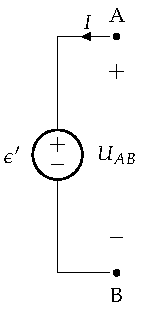
\includegraphics[height=3.5cm]{Pictures/receptor_ideal.pdf}}\hfil
			\subfigure[Real]{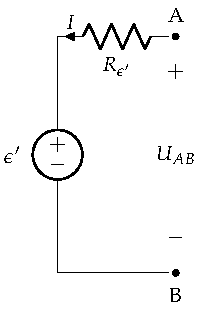
\includegraphics[height=3.5cm]{Pictures/receptor_real.pdf}}
			\caption{Receptores}
			\label{fig.receptores}
		\end{figure}
	\end{itemize}
	
	\subsubsection{El operador $D$}\label{sec.operador_D}
	Las relaciones entre tensión y corriente de resistencias, bobinas y condensadores, pueden escribirse mediante el empleo del operador $D$. Este operador es equivalente a:
	\begin{equation*}
		D\equiv \dfrac{d(...)}{dt} \rightarrow \dfrac{1}{D}=D^{-1}\equiv \int (...) dt
	\end{equation*}
	Estos operadores matemáticos permiten definir la impedancia operacional $Z(D)$, que puede representar un único elemento pasivo simple ($R$, $L$ o $C$) o una combinación de ellos. Con este concepto, la ley de Ohm es:
	\begin{equation*}
		v(t)=Z(D)\cdot i(t)
	\end{equation*}
	siendo así la impedancia un cociente entre tensión y corriente, por lo que tiene unidad de Ohmios [$\Omega$].  Con esto, las impedancias operaciones de los elementos pasivos son: 
	\begin{equation*}
		Z_R(D)=\dfrac{u_R(t)}{i(t)}=R
	\end{equation*}
	\begin{equation*}
		Z_L(D)=\dfrac{u_L(t)}{i(t)}=LD
	\end{equation*}
	\begin{equation*}
		Z_C(D)=\dfrac{u_C(t)}{i(t)}=\dfrac{1}{CD}
	\end{equation*}
	
	Análogamente, puede definirse la admitancia operacional $Y(D)$:
	\begin{equation*}
		Y(D)=\dfrac{1}{Z(D)}
	\end{equation*}
	con la que se cumple que:
	\begin{equation*}
		i(t)=Y(D)\cdot v(t)
	\end{equation*}
	La admitancia es, entonces, un cociente entre corriente y tensión, con unidad de Siemens [S]. Las admitancias operaciones de los elementos pasivos son: 
	\begin{equation*}
		Y_R(D)=\dfrac{i(t)}{u_R(t)}=\dfrac{1}{R}=G
	\end{equation*}
	\begin{equation*}
		Y_L(D)=\dfrac{i(t)}{u_L(t)}=\dfrac{1}{LD}
	\end{equation*}
	\begin{equation*}
		Y_C(D)=\dfrac{i(t)}{u_C(t)}=CD
	\end{equation*} 
	
	\begin{remark}
		Cuando los elementos pasivos son puramente reactivos, la impedancia se conoce como reactancia $X$ y, la admitancia, como susceptancia $B$.
	\end{remark}
	
	\subsection{Rendimiento}
	Cualquier máquina, dispositivo, etc., tiene un \textbf{rendimiento} (o eficiencia), que expresa el cociente entre la potencia de salida y la potencia de entrada. Puesto que todos los dispositivos/máquinas tienen pérdidas, se cumple \textbf{siempre} que el rendimiento es menor del 100\% (o 1, si se expresa en tanto por uno). En general, para la teoría de circuitos, interesa conocer el rendimiento de:
	\begin{itemize}
		\item Generadores:
		\begin{equation}
			\boxed{\eta_g (\%) = \frac{P_{u}}{P_{g}}\cdot 100}
		\end{equation}
		\item Receptores (fundamentalmente, motores):
		\begin{equation}
			\boxed{\eta_m (\%) = \frac{P_{u}}{P_{a}}\cdot 100}
		\end{equation}
	\end{itemize}
	
	
	\section{Leyes de Kirchhoff}
	
	\subsection{Definiciones}
	Existen una serie de definiciones previas que es necesario conocer para el análisis y la teoría de circuitos eléctricos:
	\begin{itemize}
		\item \textbf{Nudo:} unión de \textbf{3} o más conductores
		\item \textbf{Rama:} elementos conectados entre dos nudos consecutivos
		\item \textbf{Lazo:} conjunto de ramas que forman un camino cerrado
		\item \textbf{Malla:} lazo que no contiene ningún otro en su interior
	\end{itemize}
	
	\vspace{4mm}
	\begin{example}\label{ej.1-3}
		\textbf{Determinar el número de nudos, ramas, lazos y mallas del circuito de la Figura~\ref{fig.mallas}.}
		\begin{figure}[htbp]
			\centering
			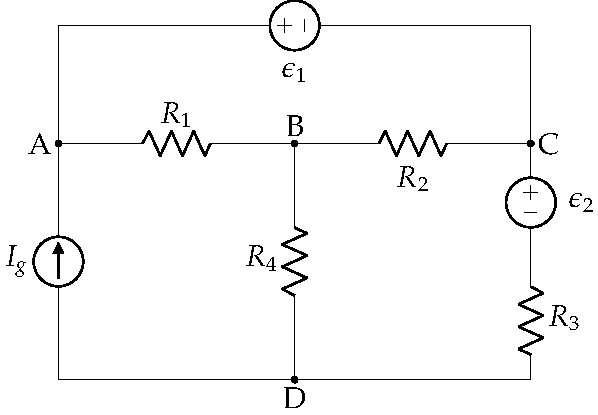
\includegraphics[width=0.4\linewidth]{Pictures/mallas.pdf}
			\caption{Ejercicio~\ref{ej.1-3}}
			\label{fig.mallas}
		\end{figure}
		
		Nudos: 4 (A, B, C, D)
		
		Ramas: 6 (AB, AC, AD, BC, BD, DC)
		
		Lazos: 7 (ABDA, BCDB, ACBA, ABCDA, ACBDA, BDCAB, ACDA) 
		
		Mallas: 3 (ABDA, BCDB, ACBA)
	\end{example}
	
	
	Aún era un estudiante cuando en 1845 Gustav Robert Kirchhoff, a la edad de 21 años, realizó la primera de sus grandes aportaciones a la física, formulando las ahora denominadas \textbf{leyes de Kirchhoff}, ecuaciones básicas de los circuitos eléctricos.
	
	\begin{itemize}
		\item \textbf{Primera ley de Kirchhoff}. Esta ley es el resultado directo del \textbf{principio de conservación de la carga} aplicado a los circuitos eléctricos. Se conoce como primera ley de Kirchhoff (1LK) o ley de Kirchhoff de las corrientes (LKC), y dice que la suma algebráica de las intensidades de corriente que concurren en un nudo es cero. Esto es igual a decir que la suma de las corrientes que llegan a un nudo es igual a la suma de las que salen: 
		\begin{equation}
			\boxed{\sum_{i=1}^n i_i(t)=0}
		\end{equation}
		Así, en la Figura~\ref{fig.LKC_FM} se cumple que:
		\begin{equation*}
			i_1(t) - i_2(t) + i_3(t) - i_4(t) + i_5(t) = 0
		\end{equation*}
		
		\begin{figure}[htbp]
			\centering
			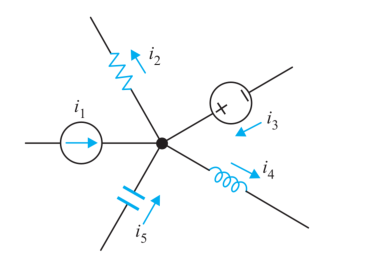
\includegraphics[width=0.35\linewidth]{Pictures/LKC_FM.pdf}
			\caption{Primera ley de Kirchhoff}
			\label{fig.LKC_FM}
		\end{figure}
		\item \textbf{Segunda ley de Kirchhoff.} Esta ley es consecuencia del \textbf{principio de conservación de la energía} aplicado a los circuitos eléctricos. Se le
		denomina segunda ley de Kirchhoff (2LK) o ley de Kirchhoff de los voltajes (LKV), y dice que la suma (con signo) de las tensiones a lo largo de un circuito cerrado es cero. Esto quiere decir que la energía producida por un generador es consumida por los receptores del circuito
		para producir algún tipo trabajo (mecánico, químico, etc.) o calor:
		\begin{equation}
			\boxed{\sum_{j=1}^m u_i(t)=0}
		\end{equation}
		Así, en el circuito de la Figura~\ref{fig.LKV_FM}, se cumple que:
		\begin{equation*}
			u_3(t) + u_4 (t) - u_5 (t) - u_1 (t) - u_2 (t)  = 0 
		\end{equation*}
		\begin{figure}[htbp]
			\centering
			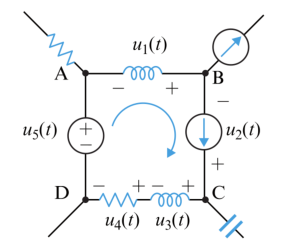
\includegraphics[width=0.35\linewidth]{Pictures/LKV_FM.pdf}
			\caption{Segunda ley de Kirchhoff}
			\label{fig.LKV_FM}
		\end{figure}
	\end{itemize}
	
	\subsection{Balance de tensiones: ecuación de una rama y ley de Ohm para un circuito cerrado}
	\begin{figure}[tbp]
		\centering
		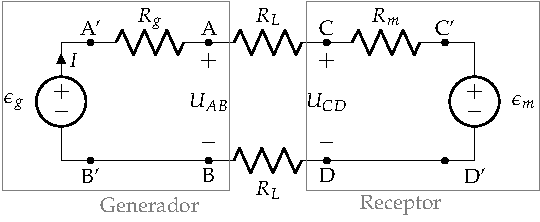
\includegraphics[width=0.5\linewidth]{Pictures/circuito_lkv.pdf}
		\caption{Ecuación de una rama}
		\label{fig.circuito_lkv}
	\end{figure}
	Escribir la ecuación de una rama implica \textbf{determinar la diferencia de potencial que tiene aplicada}. Considérese el circuito de la Figura~\ref{fig.circuito_lkv}. Se cumple que, en las ramas $AB$ y $CD$: 
	\begin{equation*}
		U_{AB} = U_{AA'} + U_{A'B'} + U_{B'B}; \qquad
		U_{CD} = U_{CC'} + U_{C'D'} + U_{D'D}
	\end{equation*}
	y, aplicando la Ley de Ohm a cada resistencia:
	\begin{equation*}
		U_{A'A} = I \cdot R_g; \qquad
		U_{AC} = I \cdot R_L; \qquad 
		U_{CC'} = I \cdot R_m; \qquad
		U_{DB} = I \cdot R_L
	\end{equation*}
	Las tensiones $U_{D'D}= U_{BB'} = 0$, dado que no hay ningún elemento conectado entre ellos y, por tanto, no hay diferencia de potencial. Por último, en los generadores $\epsilon_g$ y $\epsilon_m$, se cumple que:
	\begin{equation*}
		U_{C'D'} = \epsilon_m;\qquad
		U_{B'A'} = -\epsilon_g
	\end{equation*}
	Por tanto: 
	\begin{equation*}
		U_{AB} = U_{AA'} + U_{A'B'} + \cancel{U_{B'B}}=-U_{A'A}-U_{A'B}=-I \cdot R_g-(-\epsilon_g)=\epsilon_g-I \cdot R_g% \rightarrow   {U_{AB} = \epsilon_g - I \cdot R_g}
	\end{equation*}
	
	\begin{equation*}
		U_{CD} = U_{CC'} + U_{C'D'} + \cancel{U_{D'D}}=I \cdot R_m +\varepsilon_m%\rightarrow {U_{CD} = \epsilon_m + I\cdot R_m}
	\end{equation*}
	En general, puede decirse que la diferencia de potencial de una rama es igual al producto de la intensidad que circula por ella por la suma de todas las resistencias que contiene, menos la suma algebraica de todas la
	fuerzas electromotrices, consideradas positivas ($+$) las que tienden a crear corriente en el sentido que se recorre la rama y negativas ($-$) en caso contrario:
	\begin{equation}\label{eq.ecuacion_rama}
		\boxed{U=I\cdot \sum_{i=1}^n R_i-\sum_{j=1}^m \varepsilon_j}
	\end{equation}
	
	Considerando ahora el circuito cerrado, tal como se muestra en la Figura~\ref{fig.circuito_lkv}, aplicando la 2LK: 
	\begin{equation*}
		U_{A'A} + U_{AC} + U_{CC'} + U_{C'D'} + \cancel{U_{D'D}} + U_{DB} + \cancel{U_{BB'}} + U_{B'A'} = I \cdot R_g+I \cdot R_L+I \cdot R_m+\epsilon_m+I \cdot R_L-\epsilon_g=0
	\end{equation*}
	Por tanto, despejando la $I$ de la expresión anterior, se llega a:
	\begin{equation*}
		I=\dfrac{\epsilon_g-\epsilon_m}{R_g + 2\cdot R_L + R_m}
	\end{equation*}
	Generalizando esta ecuación, se obtiene la conocida Ley de Ohm para un circuito cerrado, considerando las f.e.m. positivas ($+$) si tienden a crear corriente en el sentido que se recorre la malla, y negativas ($-$) en caso contrario:
	\begin{equation}
		\boxed{I=\dfrac{\displaystyle\sum_{j=1}^m \varepsilon_j}{\displaystyle\sum_{i=1}^n R_i}}
	\end{equation}
	
	\subsection{Asociación de elementos}
	
	Los diferentes elementos (tanto los activos como los pasivos) se pueden asociar de diferentes formas según la conexión que se haga entre ellos. 
	
	\subsubsection{Conexión en serie}
	Se dice que dos o más elementos están acoplados en \textbf{serie} cuando el final del primero se conecta al principio del segundo, el final del segundo al principio del tercero, y así sucesivamente. Es decir, varios elementos están conectados en serie cuando por ellos circula la \textbf{misma corriente}. 
	
	\begin{itemize}
		\item \textbf{Resistencias.} Siguiendo el circuito de la Figura~\ref{fig.serie}, se cumple que:
		\begin{align*}
			u_1(t) &= R_1 \cdot i(t)\\
			u_2(t) &= R_2 \cdot i(t)\\
			u_3(t) &= R_3 \cdot i(t)
		\end{align*}
		\begin{figure}[htbp]
			\centering
			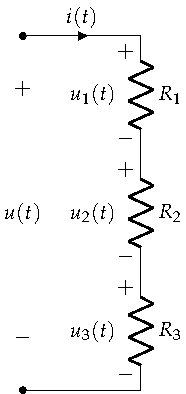
\includegraphics[width=0.2\linewidth]{Pictures/AsociacionSerie.pdf}
			\caption{Conexión de resistencias en serie}
			\label{fig.serie}
		\end{figure}
		Al aplicar la 2LK, se obtiene que: 
		\begin{equation*}
			u(t) = u_1(t) + u_2(t) + u_3(t)
		\end{equation*}
		y sacando $i(t)$ como factor común, queda:
		\begin{equation*}
			u(t) = i(t) \cdot (R_1 + R_2 + R_3)
		\end{equation*}
		Por tanto, se puede definir la resistencia equivalente $R_{eq}$ de la conexión en serie como:
		\begin{equation}
			\boxed{R_{eq} = \sum_{i = 1}^n R_i}
		\end{equation}
		de modo que:
		\begin{equation*}
			u(t) = R_{eq} \cdot i(t)
		\end{equation*}
		
		Además, de las ecuaciones anteriores se tiene:
		\begin{align*}
			i(t) = \dfrac{u(t)}{R_1 + R_2 + R_3}
		\end{align*}
		pudiendo calcular la tensión de cualquiera de las resistencias como: 
		\begin{equation*}
			u_i(t) = R_i \cdot i(t)
		\end{equation*}
		Por tanto, la tensión parcial $u_i(t)$ se puede expresar en función de la tensión total $u(t)$ como: 
		\begin{equation*}
			u_i(t) = u(t) \cdot \frac{R_i}{R_1 + R_2 + R_3}
		\end{equation*}
		conocido como \textbf{divisor de tensión}. En general, para un circuito en serie:
		\begin{equation}
			\boxed{u_i(t) = u(t) \cdot \frac{R_i}{R_{eq}}}
		\end{equation}
		\item \textbf{Bobinas.} Siguiendo el circuito de la Figura~\ref{fig.bobinas-serie}, se cumple que:
		\begin{align*}
			u_1(t) &= L_1 \cdot \dfrac{di(t)}{dt}\\
			u_2(t) &= L_2 \cdot \dfrac{di(t)}{dt}\\
			u_3(t) &= L_3 \cdot \dfrac{di(t)}{dt}\\
		\end{align*}
		\begin{figure}[htbp]
			\centering
			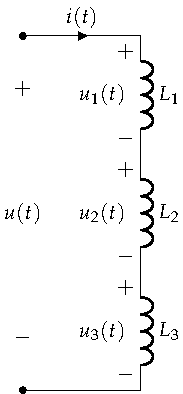
\includegraphics[width=0.2\linewidth]{Pictures/BobinasSerie.pdf}
			\caption{Conexión de bobinas en serie}
			\label{fig.bobinas-serie}
		\end{figure}
		De manera análoga a las resistencias, al aplicar la 2LK se obtiene que: 
		\begin{equation*}
			u(t) = u_1(t) + u_2(t) + u_3(t)
		\end{equation*}
		y sacando $\frac{di(t)}{dt}$ como factor común, queda:
		\begin{equation*}
			u(t) = \dfrac{di(t)}{dt} \cdot (L_1 + L_2 + L_3)
		\end{equation*}
		por lo que se puede definir la inductancia equivalente $L_{eq}$ de la conexión en serie como:
		\begin{equation}
			\boxed{L_{eq} = \sum_{i = 1}^n L_i}
		\end{equation}
		de modo que:
		\begin{equation*}
			u(t) = L_{eq} \cdot \dfrac{di(t)}{dt}
		\end{equation*}
		\item \textbf{Condensadores.} Con el circuito de la Figura~\ref{fig.condensadores-serie}, se cumple que:
		\begin{align*}
			i(t) &= C_1 \cdot \frac{du_1(t)}{dt}\\
			i(t) &= C_2 \cdot \frac{du_2(t)}{dt}\\
			i(t) &= C_3 \cdot \frac{du_3(t)}{dt}\\
		\end{align*}
		\begin{figure}[htbp]
			\centering
			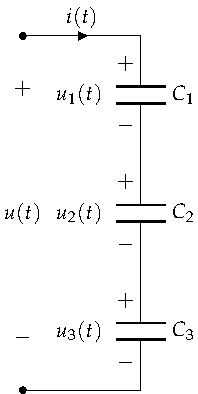
\includegraphics[width=0.2\linewidth]{Pictures/CondensadoresSerie.pdf}
			\caption{Conexión de condensadores en serie}
			\label{fig.condensadores-serie}
		\end{figure}
		Al aplicar la 2LK se obtiene que: 
		\begin{equation*}
			u(t) = u_1(t) + u_2(t) + u_3(t)
		\end{equation*}
		Suponiendo que la carga sea nula en el instante inicial (para que las constantes de integración sean nulas) y sacando factor común $\int i(t)\,dt$, se tiene:
		\begin{equation*}
			u(t)=\left(\dfrac{1}{C_1}+\dfrac{1}{C_2}+\dfrac{1}{C_3} \right)\cdot \int i(t) dt
		\end{equation*}
		por lo que se puede definir la capacidad equivalente $C_{eq}$ de la conexión en serie como:
		\begin{equation}
			\boxed{\dfrac{1}{C_{eq}} = \sum_{i = 1}^n \dfrac{1}{C_i}}
		\end{equation}
		de modo que:
		\begin{equation*}
			i(t) = C_{eq} \cdot \frac{du(t)}{dt}
		\end{equation*}
		\item \textbf{Fuentes de tensión.} Pueden conectarse en serie sin que exista \textbf{ninguna restricción}, independientemente de que se considere su modelo ideal o real. Su f.e.m. equivalente será la suma de cada una de las f.e.m.s. (por la 2LK) y, la resistencia equivalente, la suma de las resistencias internas de cada generador (en caso de considerar el modelo real).
		\item \textbf{Fuentes de corriente.} Hay que hacer diferencia entre si se considera el modelo ideal o el real:
		\begin{itemize}
			\item \textbf{Ideal.} Las fuentes de corriente ideales pueden conectarse en serie si, y sólo si, todas las fuentes suministran \textbf{igual intensidad y en el mismo sentido} (por la 1LK).
			\item \textbf{Real.} No existe ninguna restricción, llegando al generador equivalente mediante trasformación de fuentes (ver Sección~\ref{sec.dualidad}). 
		\end{itemize}
	\end{itemize}
	
	\subsubsection{Conexión en paralelo}
	Se dice que dos o más elementos están acoplados en \textbf{paralelo} cuando todos los principios están conectados a un mismo punto, y todos los finales lo están en otro. Es decir, varios elementos están conectados en paralelo cuando todos ellos se encuentran sometidos a la \textbf{misma diferencia de potencial}.
	
	\begin{itemize}
		\item \textbf{Resistencias.} Con el circuito de la Figura~\ref{fig.resistencias-paralelo}, se cumple que:
		\begin{align*}
			i_1(t) &= \dfrac{u(t)}{R_1}\\
			i_2(t) &= \dfrac{u(t)}{R_2}\\
			i_3(t) &= \dfrac{u(t)}{R_3}\\
		\end{align*}
		\begin{figure}[tbp]
			\centering
			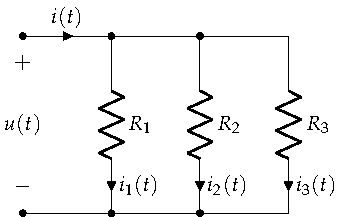
\includegraphics[width=0.35\linewidth]{Pictures/AsociacionParalelo.pdf}
			\caption{Conexión de resistencias en paralelo}
			\label{fig.resistencias-paralelo}
		\end{figure}
		Al aplicar la 1LK, se obtiene que: 
		\begin{equation*}
			i(t) = i_1(t) + i_2(t) + i_3(t)
		\end{equation*}
		y sacando $u(t)$ como factor común, queda:
		\begin{equation*}
			i(t) = u(t) \cdot \left(\frac{1}{R_1} + \frac{1}{R_2} + \frac{1}{R_3}\right)
		\end{equation*}
		Por tanto, se puede definir la resistencia equivalente $R_{eq}$ de la conexión en paralelo como:
		\begin{equation}
			\boxed{\dfrac{1}{R_{eq}} = \sum_{i = 1}^n \dfrac{1}{R_i}}
		\end{equation}
		de modo que:
		\begin{equation*}
			u(t) = R_{eq} \cdot i(t)
		\end{equation*}
		
		\begin{remark}
			En el caso concreto de \textbf{dos resistencias} en paralelo, la expresión sería: 
			\begin{equation*}
				R_{eq}=\dfrac{1}{\frac{1}{R_1}+\frac{1}{R_2}}=\dfrac{1}{\frac{R_2+R_1}{R_1\cdot R_2}}=\dfrac{R_1\cdot R_2}{R_1+R_2}
			\end{equation*}
		\end{remark}
		
		Como se mencionó en la Sección~\ref{sec.elementos_pasivos}, se define la \textbf{conductancia} $G$ [S] como la inversa de la resistencia. Así, en lugar de:
		\begin{equation*}
			\dfrac{1}{R_{eq}} = \sum_{i = 1}^n \dfrac{1}{R_i}
		\end{equation*}
		\begin{equation*}
			u(t) = R_{eq} \cdot i(t)
		\end{equation*}
		se puede escribir:
		\begin{equation}
			\boxed{G_{eq} = \sum_{i = 1}^n G_i}
		\end{equation}
		\begin{equation*}
			i(t) = G_{eq} \cdot u(t)
		\end{equation*}
		
		Además, de las ecuaciones anteriores (usando la conductancia) se tiene:
		\begin{align*}
			u(t) = \dfrac{i(t)}{G_1 + G_2 + G_3}
		\end{align*}
		pudiendo calcular la corriente de cualquiera de las resistencias como: 
		\begin{equation*}
			i_i(t) = G_i \cdot u(t)
		\end{equation*}
		Por tanto, la corriente parcial $i_i(t)$ se puede expresar en función de la corriente total $i(t)$ como: 
		\begin{equation*}
			i_i(t) = i(t) \cdot \dfrac{G_i}{G_1 + G_2 + G_3}
		\end{equation*}
		conocido como \textbf{divisor de corriente}. En general, para un circuito en paralelo:
		\begin{equation}
			\boxed{i_i(t) = i(t) \cdot \frac{G_i}{G_{eq}}}
		\end{equation}
		\item \textbf{Bobinas.} Considerando el circuito de la Figura~\ref{fig.bobinas-paralelo}, se cumple que:
		\begin{align*}
			u(t) &= L_1 \cdot \frac{di_1(t)}{dt}\\
			u(t) &= L_2 \cdot \frac{di_2(t)}{dt}\\
			u(t) &= L_3 \cdot \frac{di_3(t)}{dt}\\
		\end{align*}
		\begin{figure}[htbp]
			\centering
			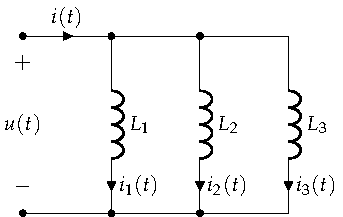
\includegraphics[width=0.35\linewidth]{Pictures/BobinasParalelo.pdf}
			\caption{Conexión de bobinas en paralelo}
			\label{fig.bobinas-paralelo}
		\end{figure}
		Al aplicar la 1LK, se obtiene que: 
		\begin{equation*}
			i(t) = i_1(t) + i_2(t) + i_3(t)
		\end{equation*}
		y, suponiendo que la carga sea nula en el instante inicial (para que las constantes de integración sean nulas) y sacando factor común $\int u(t)\,dt$, se tiene:
		\begin{equation*}
			i(t)=\left(\dfrac{1}{L_1}+\dfrac{1}{L_2}+\dfrac{1}{L_3} \right)\cdot \int u(t) dt
		\end{equation*}
		Por tanto, se puede definir la inductancia equivalente $L_{eq}$ de la conexión en paralelo como:
		\begin{equation}
			\boxed{\dfrac{1}{L_{eq}} = \sum_{i = 1}^n \dfrac{1}{L_i}}
		\end{equation}
		de manera que:
		\begin{equation*}
			u(t) = L_{eq} \cdot \dfrac{di(t)}{dt}
		\end{equation*}
		\item \textbf{Condensadores.} Con el circuito de la Figura~\ref{fig.condensadores-paralelo}, se cumple que:
		\begin{align*}
			i_1(t) &= C_1 \cdot \frac{du(t)}{dt}\\
			i_2(t) &= C_2 \cdot \frac{du(t)}{dt}\\
			i_3(t) &= C_3 \cdot \frac{du(t)}{dt}\\
		\end{align*}
		\begin{figure}[htbp]
			\centering
			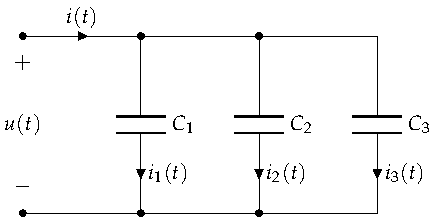
\includegraphics[width=0.4\linewidth]{Pictures/CondensadoresParalelo.pdf}
			\caption{Conexión de condensadores en paralelo}
			\label{fig.condensadores-paralelo}
		\end{figure}
		Al aplicar la 1LK se obtiene que: 
		\begin{equation*}
			i(t) = i_1(t) + i_2(t) + i_3(t)
		\end{equation*}
		por lo que, sacando factor común $\frac{du(t)}{dt}$, se tiene:
		\begin{equation*}
			i(t)=C_1\cdot \dfrac{du(t)}{dt}+ C_2\cdot \dfrac{du(t)}{dt}+ C_3\cdot \dfrac{du(t)}{dt}=(C_1+C_2+C_3)\cdot\dfrac{du(t)}{dt}
		\end{equation*}
		por lo que se puede definir la capacidad equivalente $C_{eq}$ de la conexión en paralelo como:
		\begin{equation}
			\boxed{C_{eq} = \sum_{i = 1}^n C_i}
		\end{equation}
		de modo que:
		\begin{equation*}
			i(t) = C_{eq} \cdot \frac{du(t)}{dt}
		\end{equation*}
		\textbf{Fuentes de tensión.} Hay que hacer diferencia entre si se considera el modelo ideal o el real:
		\begin{itemize}
			\item \textbf{Ideal.} Las fuentes de tensnión ideales pueden conectarse en serie si, y sólo si, todas las fuentes tienen \textbf{igual f.e.m. y ésta actúa en el mismo sentido}.
			\item \textbf{Real.} No existe \textbf{ninguna restricción}, llegando al generador equivalente mediante trasformación de fuentes (ver Sección~\ref{sec.dualidad}). 
		\end{itemize}
		\item \textbf{Fuentes de corriente.} Pueden conectarse en paralelo sin que exista ninguna restricción, independientemente de que se considere su modelo ideal o real. Su intensidad equivalente será la suma de cada una de las intensidades, y la resistencia equivalente se calculará a partir del paralelo entre varias resistencias (en caso de considerar el modelo real).
	\end{itemize}
	
	
	
	
	\subsubsection{Conexión estrella-triángulo}
	Estas dos configuraciones tienen una importancia fundamental en la teoría de circuitos, ya que son las dos posibilidades de conexión de cargas trifásicas. En la Figura~\ref{fig.estrella-triangulo} se muestran estas redes pasivas, cuyos terminales de acceso exterior
	se han denominado $A$, $B$ y $C$ y que tienen la misma situación ``topográfica''. La conexión triángulo está
	formada por tres resistencias $R_{ab}$, $R_{bc}$ y $R_{ca}$, que unen los diversos nudos, dando la apariencia
	geométrica de un triángulo. Por su parte, la conexión
	estrella representa tres resistencias $R_a$, $R_b$ y $R_c$, que parten de los tres nudos de acceso
	externo $A$, $B$ y $C$, y que se unen en un punto común $N$. 
	\begin{figure}[htbp]
		\centering
		\subfigure[Conexión triángulo]{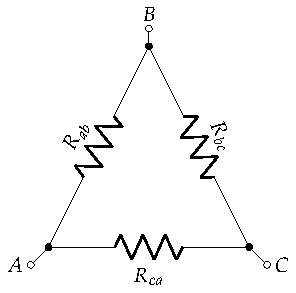
\includegraphics[width=0.3\linewidth]{Pictures/Conexion_Triangulo.pdf}}\hfil
		\subfigure[Conexión estrella]{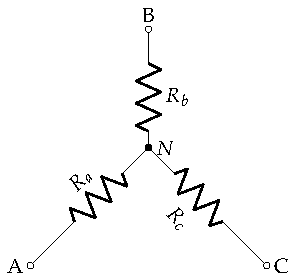
\includegraphics[width=0.3\linewidth]{Pictures/Conexion_Estrella.pdf}}
		\caption{Conexión en estrella y en triángulo}
		\label{fig.estrella-triangulo}
	\end{figure}
	
	Lo interesante es buscar las leyes de transformación de una red a la otra, de tal modo que ambos circuitos sean equivalentes desde el punto de vista externo (es decir,
	desde los nudos $A$, $B$ y $C$). Está claro que, si las dos redes son equivalentes, deberán consumir las mismas
	corrientes cuando se aplican las mismas tensiones externas, lo que equivale a decir que las resistencias que se observan entre los diferentes terminales $A-B$, $B-C$ y $C-A$ deben ser idénticas para ambos montajes y, por consiguiente, se
	deben satisfacer las igualdades mostradas en la Tabla~\ref{tab.igualdades_estrellatriangulo}. 
	\begin{table}[htbp]
		\centering
		\begin{tabular}{c|c|c}
			\rowcolor{ocre!50} \textbf{Impedancia} & \textbf{Estrella} & \textbf{Triángulo}\\
			&&        \\[-0.75em]
			$R_{AB}$ & $R_a+R_b$ & $\dfrac{R_{ab} \cdot (R_{bc} + R_{ca})}{R_{ab} + R_{bc} + R_{ca}}$\\
			&&         \\[-0.75em]
			$R_{AB}$ & $R_b+R_c$ & $\dfrac{R_{bc} \cdot (R_{ab} + R_{ca})}{R_{ab} + R_{bc} + R_{ca}}$\\
			&& \\[-0.75em]
			$R_{CA}$ & $R_a+R_c$ & $\dfrac{R_{ca} \cdot (R_{ab} + R_{bc})}{R_{ab} + R_{bc} + R_{ca}}$\\
		\end{tabular}
		\caption{Igualdades que se deben satisfacer para la equivalencia estrella-triángulo}
		\label{tab.igualdades_estrellatriangulo}
	\end{table}
	
	A partir de la Tabla~\ref{tab.igualdades_estrellatriangulo}, se obtiene que las resistencias vistas desde los diferentes nudos, en la conexión triángulo, son:
	\begin{align*}
		R_{AB} &= \frac{R_{ab} \cdot R_{bc}}{R_{ab} + R_{bc} + R_{ca}} + \frac{R_{ab} \cdot R_{ca}}{R_{ab} + R_{bc} + R_{ca}}\\
		\\
		R_{BC} &= \frac{R_{bc} \cdot R_{ab}}{R_{ab} + R_{bc} + R_{ca}} + \frac{R_{bc} \cdot R_{ca}}{R_{ab} + R_{bc} + R_{ca}}\\
		\\
		R_{CA} &= \frac{R_{ca} \cdot R_{ab}}{R_{ab} + R_{bc} + R_{ca}} + \frac{R_{ca} \cdot R_{bc}}{R_{ab} + R_{bc} + R_{ca}}
	\end{align*}
	que deben ser igual a las de estrella:
	\begin{align*}
		\dfrac{R_{a{\color{magenta}b}} \cdot R_{{\color{magenta}b}c}}{R_{ab} + R_{bc} + R_{ca}} + \dfrac{R_{{\color{teal}a}b} \cdot R_{c{\color{teal}a}}}{R_{ab} + R_{bc} + R_{ca}} &= R_{\color{teal}a} + R_{\color{magenta}b}\\
		\\
		\dfrac{R_{a{\color{magenta}b}} \cdot R_{{\color{magenta}b}c}}{R_{ab} + R_{bc} + R_{ca}} + \dfrac{R_{b{\color{orange}c}} \cdot R_{{\color{orange}c}a}}{R_{ab} + R_{bc} + R_{ca}} &= R_{\color{magenta}b} + R_{\color{orange}c}\\
		\\
		\dfrac{R_{{\color{teal}a}b} \cdot R_{c{\color{teal}a}}}{R_{ab} + R_{bc} + R_{ca}} + \dfrac{R_{b{\color{orange}c}} \cdot R_{{\color{orange}c}a}}{R_{ab} + R_{bc} + R_{ca}} &= R_{\color{orange}c} + R_{\color{teal}a}
	\end{align*}
	Igualando y operando, se llega a las siguientes relaciones: 
	\begin{itemize}
		\item \textbf{Conversión de triángulo a estrella.} 
		\begin{align*}
			R_a &= \frac{R_{ab} \cdot R_{ca}}{R_{ab} + R_{bc} + R_{ca}}\\
			\\
			R_b &= \frac{R_{ab} \cdot R_{bc}}{R_{ab} + R_{bc} + R_{ca}}\\
			\\
			R_c &= \frac{R_{bc} \cdot R_{ca}}{R_{ab} + R_{bc} + R_{ca}}
		\end{align*}
		\item \textbf{Conversión de estrella a triángulo.}
		\begin{align*}
			G_{ab} &= \frac{G_a \cdot G_b}{G_a + G_b + G_c}\\
			\\
			G_{bc} &= \frac{G_b \cdot G_c}{G_a + G_b + G_c}\\
			\\
			G_{ca} &= \frac{G_c \cdot G_a}{G_a + G_b + G_c}
		\end{align*}
	\end{itemize}
	
	Las transformaciones anteriores se utilizan con gran frecuencia en el análisis de circuitos, ya que permiten simplificar ciertas redes en las que las impedancias no están
	conectadas de forma simple (en serie o en paralelo). Quiere destacarse que, en caso de que las resistencias sean iguales ($R_a=R_b=R_c=R_Y$ para la estrella y $R_{ab}=R_{bc}=R_{ca}=R_D$ para el triángulo), se cumple que: 
	\begin{equation}
		\boxed{R_D=3\cdot R_Y}
	\end{equation}
	
	\section{Métodos de análisis}
	Para resolver un circuito, se debe conocer $U$ e $I$ en cada una de sus ramas. Por tanto, si se tiene un circuito formado por $r$ ramas, el número de incógnitas será $2\cdot r$ (una de tensión y otra de intensidad). Por tanto, para resolver el circuito se deben disponer de $2\cdot r$ ecuaciones linealmente independientes. Para ello, basta con aplicar las leyes de Kirchhoff a los nudos y mallas del circuito. 
	
	\vspace{4mm}
	\begin{example}
		\label{ej.1-4}
		\textbf{Plantear el sistema de ecuaciones para resolver el circuito de la Figura~\ref{fig.mallas1}.}
		\begin{figure}[htbp]
			\centering
			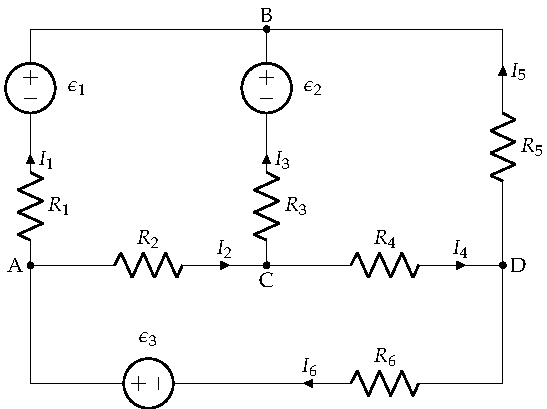
\includegraphics[width=0.35\linewidth]{Pictures/mallas1.pdf}
			\caption{Ejercicio~\ref{ej.1-4}}
			\label{fig.mallas1}
		\end{figure}
		
		\begin{enumerate}
			\item {Se aplica la 1LK:} 
			\begin{itemize}
				\item {Nudo A:} $I_6 = I_1 + I_2$
				\item {Nudo B:} $I_1 + I_3 + I_5 = 0$
				\item {Nudo C:} $I_2 = I_3 + I_4$
				\item {Nudo D:} $I_4 = I_5 + I_6$
			\end{itemize}
			Sin embargo, se observa que no son ecuaciones linealmente independientes, puesto que $C=A+B+D$.
			\item {Se aplica la 2LK:}
			\begin{itemize}
				\item {Malla ABCA:} $I_1 \cdot R_1 - \epsilon_1 + \epsilon_2 - I_3 \cdot R_3 - I_2 \cdot R_2 = 0$
				\item {Malla BDCB:} $-I_5 \cdot R_5 - I_4 \cdot R_4 + I_3 \cdot R_3 - \epsilon_2 = 0$
				\item {Malla ACDA:} $I_2 \cdot R_2 + I_4 \cdot R_4 + I_6 \cdot R_6 - \epsilon_3 = 0$
			\end{itemize}
			\item {Se combinan las ecuaciones:}
			\begin{align*}
				- I_1 -  I_2 + I_6  &= 0\\
				I_1 + I_3 + I_5 &= 0\\
				I_4 - I_5 - I_6 &= 0\\
				I_1 \cdot R_1 - I_2 \cdot R_2 - I_3 \cdot R_3 &= \epsilon_1 - \epsilon_2\\
				I_3 \cdot R_3 - I_4 \cdot R_4 -I_5 \cdot R_5 &= \epsilon_2\\
				I_2 \cdot R_2 + I_4 \cdot R_4 + I_6 \cdot R_6 &= \epsilon_3
			\end{align*}
			\item {Se expresan en forma matricial:}
			\begin{equation*}
				\begin{bmatrix}
					-1 & -1 & 0 & 0 & 0 & 1\\
					1 & 0 & 1 & 0 & 1 & 0\\
					0 & 0 & 0 & 1 & -1 & -1\\
					R_1 & -R_2 & - R_3 & 0 & 0 & 0\\
					0 & 0 & R_3 & - R_4 & - R_5 & 0\\
					0 & R_2 & 0 & R_4 & 0 & R_6
				\end{bmatrix} \cdot %
				\begin{bmatrix}
					I_1\\
					I_2\\
					I_3\\
					I_4\\
					I_5\\
					I_6    
				\end{bmatrix} = %
				\begin{bmatrix}
					0\\
					0\\
					0\\
					\epsilon_1 - \epsilon_2\\
					\epsilon_2\\
					\epsilon_3
				\end{bmatrix}
			\end{equation*}
		\end{enumerate}
		Se observa que es necesario resolver un sistema lineal de 6 ecuaciones en las que las incógnitas son las corrientes de cada rama. 
	\end{example}
	
	Esta forma de resolución de circuitos eléctricos, aunque es válida, no es útil por el número de ecuaciones a resolver. Por ello, lo más habitual es utilizar otros métodos que permiten la resolución de los circuitos con un número menor de ecuaciones. Aunque existen diferentes métodos, se van a presentar dos: el método de las mallas y el método de los nudos.
	
	\subsection{Método de las mallas}
	El método de las mallas simplifica el sistema de ecuaciones necesario mediante unas corrientes \emph{ficticias} denominadas \textbf{corrientes de malla}, aprovechando las relaciones entre corrientes de la 1LK. El procedimiento general de aplicación de este método es el siguiente:
	\begin{enumerate}
		\item Identificar las corrientes de rama.
		\item Asignar un sentido a las corrientes de malla, teniendo en cuenta que hay un total de:
		\begin{equation}
			\boxed{Mallas=Ramas-(Nudos-1)}
		\end{equation}
		\item Relacionar corrientes de rama con corrientes de malla.
		\item Escribir ecuaciones de mallas.
		\item Resolver la ecuación, obteniendo las corrientes de malla.
		\item Obtener las corrientes de rama con las relaciones del punto 3.
	\end{enumerate}
	
	\vspace{4mm}
	\begin{example}
		\label{ej.1-5}
		\textbf{Plantear el sistema de ecuaciones para resolver el circuito de la Figura~\ref{fig.mallas1}.}
		
		Se sigue el procedimiento indicado anteriormente, llegando únicamente hasta el punto 4: 
		\begin{enumerate}
			\item Identificar las corrientes de rama: están identificadas directamente en el circuito de la Figura~\ref{fig.mallas1}
			\item Asignar un sentido a las corrientes de malla: se muestra en la Figura~\ref{fig.mallas1_corrientes}
			\begin{figure}[htbp]
				\centering
				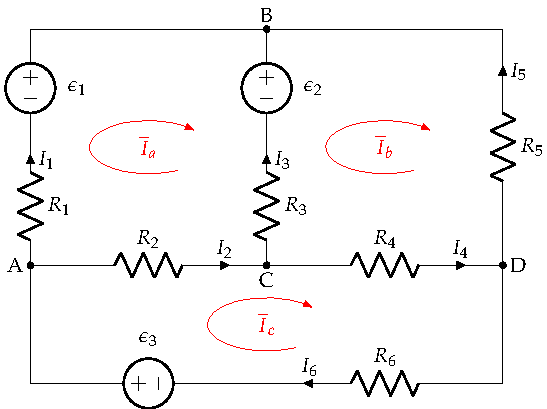
\includegraphics[width=0.35\linewidth]{Pictures/mallas1_corrientes.pdf}
				\caption{Corrientes de malla del circuito}
				\label{fig.mallas1_corrientes}
			\end{figure}
			\item Relacionar corrientes de rama con corrientes de malla:
			\begin{align*}
				I_1 &= I_a\\
				I_5 &= -I_b\\
				I_6 &= I_c\\
				I_2 &= I_c -I_a\\
				I_3 &= I_b - I_a\\
				I_4 &= I_c - I_b
			\end{align*}
			\item Escribir ecuaciones de mallas: 
			
			Malla ABCA
			\begin{equation*}
				I_a \cdot R_1 - \epsilon_1 + \epsilon_2 + (I_a - I_b) \cdot R_3 + (I_a - I_c) \cdot R_2 = 0
			\end{equation*}
			
			Malla BDCB
			\begin{equation*}
				I_b \cdot R_5 + (I_b - I_c) \cdot R_4 + (I_b - I_a) \cdot R_3 - \epsilon_2 = 0
			\end{equation*}
			
			Malla ACDA
			\begin{equation*}
				(I_c - I_a) \cdot R_2 + (I_c - I_b) \cdot R_4 + I_c \cdot R_6 - \epsilon_3 = 0
			\end{equation*}
			
			Se reagrupan las corrientes en las ecuaciones anteriores, obteniéndose que: 
			\begin{align*}
				I_a \cdot (R_1 + R_3 + R_2)  - I_b\cdot R_3 - I_c \cdot R_2 &= \epsilon_1 - \epsilon_2\\
				- I_a \cdot R_3 + I_b \cdot (R_5 + R_4 + R_3) - I_c \cdot R_4 &=  \epsilon_2\\
				- I_a \cdot R_2 - I_b \cdot R_4 + I_c \cdot (R_2 + R_4 + R_6) &= \epsilon_3
			\end{align*}
			que, en forma matricial: 
			\begin{equation*}
				\begin{bmatrix}
					(R_1 + R_3 + R_2) &  - R_3 & - R_2 \\
					- R_3 & (R_5 + R_4 + R_3) & - R_4 \\
					- R_2 & - R_4 &  (R_2 + R_4 + R_6)
				\end{bmatrix} \cdot %
				\begin{bmatrix}
					I_a\\
					I_b\\
					I_c\\
				\end{bmatrix} = %
				\begin{bmatrix}
					\epsilon_1 - \epsilon_2\\
					\epsilon_2\\
					\epsilon_3
				\end{bmatrix}
			\end{equation*}
		\end{enumerate}
	\end{example}
	
	A partir de este ejemplo, se llega a la ecuación general que permite determinar el sistema de ecuaciones de un sistema de $n$ mallas, siendo esta: 
	\begin{equation*}
		\begin{bmatrix}
			{\color{magenta}\sum R_{11}} &  {\color{teal}\pm\sum R_{12}} & {\color{teal}{\dots}} & {\color{teal}\pm\sum R_{1n}} \\
			{\color{teal}\pm\sum R_{21}} & {\color{magenta}\sum R_{22}} & {{\dots}} & {\color{teal}\pm\sum R_{2n}} \\
			{\vdots} & {\vdots} &  {\ddots} & \vdots\\
			{\color{teal}\pm\sum R_{n1}} & {\color{teal}\pm\sum R_{n2}} & \dots & {\color{magenta}\sum R_{nn}}
		\end{bmatrix} \cdot 
		\begin{bmatrix}
			I_1\\
			I_2\\
			\vdots\\
			I_n
		\end{bmatrix} = %
		\begin{bmatrix}
			{\color{orange}\sum\epsilon_1}\\
			{\color{orange}\sum\epsilon_2}\\
			{\color{orange}\vdots}\\
			{\color{orange}\sum\epsilon_n}
		\end{bmatrix}
	\end{equation*}
	donde cada {\color{magenta}$R_{ii}$} se corresponde con la suma de resistencias incluidas en la malla $i$; cada {\color{teal}$\pm R_{ij}$} se corresponde con la suma de las resistencias incluidas en las ramas compartidas por las mallas $i$ y $j$, con signo positivo ($+$) si las corrientes van en el mismo sentido, y negativo ($-$) en caso contrario; y cada {\color{orange} $\sum \epsilon_i$} es la suma algebraica de las fuerzas electromotrices de los generadores de la malla $i$, considerando un signo positivo ($+$) si contribuyen al giro de la corriente, y negativo ($-$) en caso contrario. Debe tenerse en cuenta que para aplicar este método \textbf{todos los generadores deben ser fuentes de tensión}. 
	
	\subsection{Método de los nudos}
	El método de los nudos es otro de los procedimientos de análisis utilizados en teoría de circuitos, aprovechando las relaciones entre corrientes de la 1LK. El procedimiento general de aplicación de este método es el siguiente:
	\begin{enumerate}
		\item Identificar las corrientes de rama.
		\item Identificar los nudos independientes, que son:
		\begin{equation}
			\boxed{Nudos\;\;Independientes=Nudos-1}
		\end{equation}
		\item Aplicar la 1LK a cada nudo independiente.
		\item Determinar las tensiones en los receptores a partir de la Ley de Ohm (considerando la resistencia y, después, la conductancia).
		\item Combinar las ecuaciones de los puntos 3 y 4.
		\item Resolver la ecuación.
	\end{enumerate}
	
	\vspace{4mm}
	\begin{example}\label{ej.1-6}
		\textbf{Plantear el sistema de ecuaciones para resolver el circuito de la Figura~\ref{fig.nudos}.}
		\begin{figure}[htbp]
			\centering
			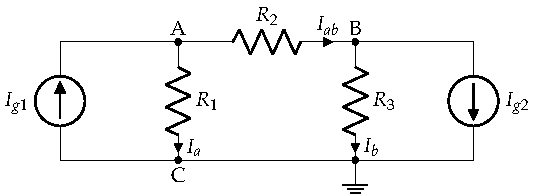
\includegraphics[width=0.6\linewidth]{Pictures/nudos.pdf}
			\caption{Ejercicio~\ref{ej.1-6}}
			\label{fig.nudos}
		\end{figure}
		
		Se sigue el procedimiento indicado anteriormente, llegando únicamente hasta el punto 5: 
		
		\begin{enumerate}
			\item Identificar las corrientes de rama: identificadas en la Figura~\ref{fig.nudos}
			\item Identificar los nudos independientes, que son $A$ y $B$ en la Figura~\ref{fig.nudos}.
			\item Aplicar la 1LK a cada nudo independiente:
			
			Nudo A
			\begin{equation*}
				I_{g1} - I_a - I_{ab} = 0
			\end{equation*}
			
			Nudo B
			\begin{equation*}
				I_{ab} - I_{g2} - I_b = 0
			\end{equation*}
			\item Determinar las tensiones en los receptores a partir de la Ley de Ohm (considerando la resistencia y, después, la conductancia):
			\begin{align*}
				U_A = U_{R_1} &= I_a \cdot R_1\rightarrow I_a=U_A\cdot G_1\\
				U_B = U_{R_3} &= I_b \cdot R_3\rightarrow I_b=U_B\cdot G_3\\
				U_{AB}=U_{R_2} &= I_{ab} \cdot R_2\rightarrow I_{ab}=(U_A-U_B)\cdot G_2\\
			\end{align*}
			\item Combinar las ecuaciones de los puntos 3 y 4:
			
			Nudo A
			\begin{equation*}
				I_{g1} - U_A \cdot G_1 - (U_A - U_B) \cdot G_2 = 0\rightarrow I_{g1} = U_A \cdot (G_1 + G_2) - U_B \cdot G_2 
			\end{equation*}
			
			Nudo B
			\begin{equation*}
				(U_A - U_B) \cdot G_2 - I_{g2} - U_B \cdot G_3 = 0 \rightarrow  - I_{g2} = - U_A \cdot G_2 + U_B \cdot (G_2 + G_3)
			\end{equation*}
			
			Estas ecuaciones se pueden expresar en forma matricial de la siguiente manera: 
			\begin{equation*}
				\begin{bmatrix}
					G_1 + G_2 & - G_2\\
					-G_2 & G_2 + G_3
				\end{bmatrix} \cdot%
				\begin{bmatrix}
					U_A\\
					U_B
				\end{bmatrix} = %
				\begin{bmatrix}
					I_{g1}\\
					-I_{g2}
				\end{bmatrix}
			\end{equation*}
		\end{enumerate}
	\end{example}
	
	A partir de este ejemplo, se llega a la ecuación general que permite determinar el sistema de ecuaciones de un sistema de $n$ nudos, siendo esta: 
	\begin{equation*}
		\begin{bmatrix}
			{\color{magenta}\sum G_{1}} &  {\color{teal}-\sum G_{12}} & {\color{teal}{\dots}} & {\color{teal}-\sum G_{1n}} \\
			{\color{teal}-\sum G_{21}} & {\color{magenta}\sum G_{2}} & {{\dots}} & {\color{teal}-\sum G_{2n}} \\
			{\vdots} & {\vdots} &  {\ddots} & \vdots\\
			{\color{teal}-\sum G_{n1}} & {\color{teal}-\sum G_{n2}} & \dots & {\color{magenta}\sum G_{n}}
		\end{bmatrix} \cdot 
		\begin{bmatrix}
			U_1\\
			U_2\\
			\vdots\\
			U_n
		\end{bmatrix} = %
		\begin{bmatrix}
			{\color{orange}\sum I_{g1}}\\
			{\color{orange}\sum I_{g2}}\\
			{\color{orange}\vdots}\\
			{\color{orange}\sum I_{gn}}
		\end{bmatrix}
	\end{equation*}
	donde cada {\color{magenta}$G_{i}$} se corresponde con la suma de conductancias conectadas al nudo $i$; cada {\color{teal}$ G_{ij}$} se corresponde con la suma de las conductancias conectadas entre los nudos $i$ y $j$; y cada {\color{orange} $\sum I_{gi}$} es la suma algebraica de las corrientes de los generadores conectados al nudo $i$, considerando un signo positivo ($+$) si el generador inyecta corriente en el nudo, y negativo ($-$) en caso contrario. Debe tenerse en cuenta que para aplicar este método \textbf{todos los generadores deben ser fuentes de corriente}. 
	
	\section{Formas de onda}
	
	En los circuitos eléctricos, las funciones de excitación y respuesta son tensiones
	e intensidades que varían con el tiempo:
	\begin{equation*}
		u=u(t)
	\end{equation*}
	\begin{equation*}
		i=i(t)
	\end{equation*}
	Estas funciones pueden representarse de forma gráfica o analítica. En ambos
	casos, esa relación funcional se conoce mediante el nombre de \textbf{forma de onda}. Las formas de onda pueden clasificarse según (de manera análoga a lo indicado en la Sección~\ref{sec.cc-ca}):
	\begin{itemize}
		\item \textbf{Signo de la magnitud}:
		\begin{itemize}
			\item \textbf{Unidireccionales}: la magnitud que la representa siempre tiene una única polaridad (signo constante, aunque el valor puede ser constante o variable)
			\item \textbf{Bidireccionales}: la magnitud toma valores positivos y negativos (signo variable con el tiempo)
		\end{itemize}
		\item \textbf{Repetición del valor de la magnitud}:
		\begin{itemize}
			\item \textbf{Periódicas}: el valor de la magnitud se repite de forma regular
			\item \textbf{No periódicas}: el valor de la magnitud varía de forma arbitraria con el tiempo
		\end{itemize}
	\end{itemize}
	
	\subsection{Formas de onda básicas}
	En el estudio de la teoría de circuitos, son de especial interés las formas de onda en escalón, rampa, pulsos y triangular.
	
	\subsubsection{Función escalón} 
	Esta función vale 0 para tiempos negativos ($t<0$) y un valor constante $K$ para tiempos positivos ($t>0$), como se muestra en la Figura~\ref{fig.escalon}. Por tanto, su expresión matemática es: 
	\begin{equation}
		\boxed{f(t) = %
			\begin{cases}
				0 & t < 0\\
				K & t \geq 0
		\end{cases}}
	\end{equation}
	
	\begin{figure}[htbp]
		\centering
		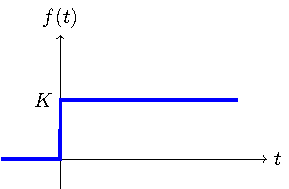
\includegraphics[width=.35\linewidth]{Pictures/escalon.pdf}
		\caption{Función escalón en el origen de tiempos}
		\label{fig.escalon}
	\end{figure}
	
	Cuando $K = 1$, la función recibe el nombre de \textbf{escalón unitario}. En general, se puede considerar cualquier función escalón como el producto de una constante (denominada \textit{amplitud}) por la función escalón unitario.
	En general, multiplicar una función por la función escalón unitario se asocia a asignar el valor 0 para $t<0$ y no modifica la función para $t>0$.
	
	\subsubsection{Función pulso rectangular}
	
	Esta forma de onda es muy habitual en electrónica, y se representa en la Figura~\ref{fig.pulso}. Su expresión matemática viene dada por:
	\begin{equation}
		\boxed{f(t) = %
			\begin{cases}
				0 & t < 0\\
				K & 0 \leq t \leq W\\
				0 & t>W
		\end{cases}}
	\end{equation}
	\begin{figure}[htbp]
		\centering
		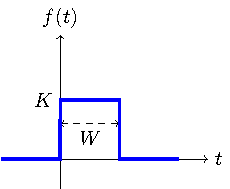
\includegraphics[width=.35\linewidth]{Pictures/pulso.pdf}
		\caption{Función pulso rectangular}
		\label{fig.pulso}
	\end{figure}
	
	El valor $W$ se conoce como \textbf{anchura/duración del pulso}. 
	
	\subsubsection{Función rampa}
	La forma de esta función es la indicada en la Figura~\ref{fig.rampa}, expresada de manera matemática de la siguiente forma: 
	\begin{equation}
		\boxed{f(t) = %
			\begin{cases}
				0 & t < 0\\
				m \cdot t  & t \geq 0
		\end{cases}}
	\end{equation}
	\begin{figure}[htbp]
		\centering
		\includegraphics[width=0.35\linewidth]{Pictures/rampa.pdf}
		\caption{Función rampa}
		\label{fig.rampa}
	\end{figure}
	El valor de $m$ es la pendiente de la rampa.
	
	\subsubsection{Función triangular}
	La forma de esta función es la indicada en la Figura~\ref{fig.triangular}, expresada de manera matemática de la siguiente forma: 
	\begin{equation}
		\boxed{
			f(t) = %
			\begin{cases}
				0 & t < -W/2\\
				m \cdot (t + W/2)  & -W/2 \leq t \leq 0\\
				-m \cdot (t - W/2)  & 0 \leq t \leq W/2\\
				0  & t > W/2
		\end{cases}}
	\end{equation}
	\begin{figure}[htbp]
		\centering
		\includegraphics[width=0.35\linewidth]{Pictures/triangular.pdf}
		\caption{Función triangular}
		\label{fig.triangular}
	\end{figure}
	
	\subsubsection{Retraso del origen de tiempos}
	Una forma de onda puede retrasarse en el tiempo si se desplaza el eje de ordenadas en una cantidad $-t_0$. La Figura~\ref{fig.retraso} muestra diversos ejemplos de las formas de onda básicas. 
	\begin{figure}[htbp]
		\centering
		\subfigure[Escalón retrasado]{\includegraphics[width=.35\linewidth]{Pictures/escalon_t0.pdf}}\hfil
		\subfigure[Pulso retrasado]{\includegraphics[width=.35\linewidth]{Pictures/pulso_t0.pdf}}\\
		\subfigure[Rampa retrasada]{\includegraphics[width=.35\linewidth]{Pictures/rampa_t0.pdf}}\hfil
		\subfigure[Triangular retrasada]{\includegraphics[width=.35\linewidth]{Pictures/triangular_t0.pdf}}
		\caption{Formas de onda básicas retrasadas}
		\label{fig.retraso}
	\end{figure}
	
	\subsection{Formas de onda periódicas}
	Son aquellas formas de onda cuyos valores se repiten a intervalos iguales de tiempo y en el mismo orden:
	\begin{equation*}
		y(t)=y(t+T)=y(t+n\cdot T)
	\end{equation*}
	
	\subsubsection{Definiciones y valores de interés de las ondas periódicas}
	Existen una serie de definiciones y valores de interés para las ondas periódicas:
	\begin{itemize}
		\item \textbf{Período ($T$)}: intervalo de tiempo mínimo a partir del cual se repite la forma de onda [s]
		\item \textbf{Frecuencia ($f$)}: número de veces que se repite la onda por unidad de tiempo [Hz]:
		\begin{equation*}
			f = \dfrac{1}{T}
		\end{equation*}
		\item \textbf{Valor instantáneo}: valor $y(t)$ que toma la forma de onda en un instante de tiempo dado
		\item \textbf{Valores de pico ($Y_{max}$, $Y_{min}$)}: valores máximo y mínimo que toma la forma de onda en un periodo:
		\begin{equation*}
			Y_{max} = \max(f(t)); \qquad Y_{min} = \min(f(t))
		\end{equation*}
		\item \textbf{Valor pico a pico ($Y_{PP}$)}: se corresponde con la diferencia (en valor absoluto) entre los valores de pico considerados con signo: 
		\begin{equation*}
			Y_{PP}=|Y_{max} - Y_{min}|
		\end{equation*}
		\item \textbf{Valor medio ($Y_m$)}: en un intervalo ($t_1,t_2$), corresponde con la media aritmética de los valores instantáneos que toma la función en dicho intervalo:
		\begin{equation*}
			Y_m=\dfrac{1}{t_2-t_1}\cdot\int_{t_1}^{t_2}y(t)\, dt
		\end{equation*}
		En una onda periódica, se calcula para un intervalo de tiempo igual a un periodo: 
		\begin{equation}\label{eq.valor_medio}
			\boxed{Y_m=\frac{1}{T}\int_{a}^{a+T}y(t)\, dt}
		\end{equation}
		\begin{remark}
			En caso de que el valor medio sea nulo en un periodo, el cálculo se realiza en un semi-periodo ($T/2$) o en un cuarto de periodo ($T/4$)
		\end{remark}
		\item \textbf{Valor eficaz ($Y_{ef}$)}: es la raíz cuadrada de la media de los cuadrados de los valores que toma la función en un intervalo:
		\begin{equation*}
			Y_{ef}=\sqrt{\dfrac{1}{t_2-t_1}\cdot\int_{t_1}^{t_2}y^2(t)\, dt}
		\end{equation*}
		Si es periódica: 
		\begin{equation}
			\boxed{Y_{ef} = \sqrt{\frac{1}{T}\cdot\int_{a}^{a+T}y^{2}(t)\, dt}}
		\end{equation}
		\item \textbf{Factor de amplitud ($FA$)}: es el cociente entre el valor máximo y el valor eficaz de una onda:
		\begin{equation*}
			FA = \dfrac{Y_{max}}{Y_{ef}}
		\end{equation*}
		\item \textbf{Factor de forma ($FF$)}: es el cociente entre el valor eficaz y el valor medio:
		\begin{equation*}
			FF = \dfrac{Y_{ef}}{Y_{m}}
		\end{equation*}
		\begin{remark}
			Si el valor medio fuese nulo en un período, se toma el de un semiperíodo
		\end{remark}
	\end{itemize}
	
	\subsubsection{Función sinusoidal}\label{sec.sinusoidal}
	Dentro de las ondas periódicas, las \textbf{ondas sinusoidales} son de gran importancia en el campo de la electricidad. Estas formas de onda vienen determinadas por:
	\begin{equation}
		\boxed{y(t)=Y_{max}\cdot\sin(\omega t+\theta)} 
	\end{equation}
	siendo $Y_{max}$ el valor máximo de la onda, $\omega$ la pulsación o frecuencia angular [rad/s] ($\omega=2\cdot\pi\cdot f$, siendo $f$ la frecuencia de la onda [Hz]) y $\theta$ la fase [rad o $^\circ$]. Un ejemplo de este tipo de forma de onda se muestra en la Figura \ref{fig.sin}.
	\begin{figure}[htbp]
		\centering
		\includegraphics[width=.9\linewidth]{Pictures/sin.pdf}
		\caption{Ejemplo de forma de onda sinusoidal}
		\label{fig.sin}
	\end{figure}
	
	Las propiedades de las formas de onda senoidales que hacen que sea la preferida para la generación de energía eléctrica a gran escala son las siguientes:
	\begin{enumerate}
		\item Su forma básica se mantiene siempre, puesto que sus derivadas e integrales sucesivas son funciones sinusoidales $\rightarrow$ si la excitación es sinusoidal, las respuestas también son (pasado un corto periodo de tiempo transitorio)
		\item La suma o resta de funciones senoidales de la misma frecuencia es otra función senoidal de la misma frecuencia
	\end{enumerate}
	Respecto al estudio de otras formas de onda, su interés reside en el teorema de Fourier, dado que cualquier onda periódica no senoidal puede suponerse formada por
	infinitas ondas senoidales de distinta frecuencia. 
	
	Al ser un caso particular de una onda periódica, las definiciones y valores de interés indicados previamente también son válidos. Por simplicidad, se considera la función sinusoidal con fase inicial nula, $y(t)=Y_{max}\cdot\sin(\omega t)$:
	\begin{itemize}
		\item \textbf{Valor pico a pico ($Y_{PP}$)}: es el doble de la amplitud: 
		\begin{equation*}
			Y_{PP}=|Y_{max} - Y_{min}|=2\cdot Y_{max}
		\end{equation*}
		\item \textbf{Valor medio ($Y_m$)}: en un periodo, el valor medio es 0, puesto que el área positiva es igual al área negativa. Considerando entonces un semiperíodo: 
		\begin{equation*}
			Y_m(T/2)=\frac{1}{T/2}\int_{0}^{T/2} Y_{max}\cdot \sin(\omega t)\, dt=\dfrac{2\cdot Y_{max}}{T\cdot\omega}\left[-\cos(\omega\cdot t)\right]_0^{T/2} =\dfrac{2\cdot Y_{max}}{\pi}\approx 0.637\cdot Y_{max}
		\end{equation*}
		\item \textbf{Valor eficaz ($Y_{ef}$)}: para simplificar el cálculo, se hace en primer lugar el valor eficaz al cuadrado:
		\begin{equation*}
			Y_{ef}^2=\dfrac{1}{T}\cdot\int_{0}^{T}\left(Y_{max}\cdot\sin(\omega  t)\right)^{2}\,dt=\dfrac{Y_{max}^2}{T}\cdot\int_{0}^{T}\left(\sin(\omega t)\right)^{2}\,dt=\dfrac{Y_{max}^2}{2}
		\end{equation*}
		luego:
		\begin{equation*}
			Y_{ef}=\sqrt{Y_{ef}^2}=\dfrac{Y_{max}}{\sqrt{2}}\approx0.707\cdot Y_{max}
		\end{equation*}
		\item \textbf{Factor de amplitud ($FA$)}: 
		\begin{equation*}
			FA = \dfrac{Y_{max}}{Y_{ef}}=\dfrac{\cancel{Y_{max}}}{\frac{\cancel{Y_{max}}}{\sqrt{2}}}=\sqrt{2}\approx 1.414
		\end{equation*}
		\item \textbf{Factor de forma ($FF$)}: 
		\begin{equation*}
			FF = \dfrac{Y_{ef}}{Y_{m}} = \dfrac{\frac{\cancel{Y_{max}}}{\sqrt{2}}}{\frac{2\cdot \cancel{Y_{max}}}{\pi}}=\dfrac{\pi}{2\cdot\sqrt{2}}\approx 1.111
		\end{equation*}
	\end{itemize}
	
	\subsubsection{Interpretación fasorial de una función sinusoidal}
	
	Cuando se trabaje con corriente alterna, siempre se usarán funciones de onda sinusoidales, todas ellas a la misma pulsación $\omega$. Por tanto, las diferencias que habrá en dichas ondas serán, únicamente, las amplitudes $Y_{max}$ y las fases $\theta$. Esto permite que, en lugar de trabajar con formas de onda, se pueda trabajar con \textbf{fasores}. Un fasor es un vector giratorio, anclado en el origen del plano complejo, que gira en el sentido contrario a las agujas del reloj a velocidad angular constante $\omega$. La longitud del fasor (su módulo) es el \textbf{valor eficaz} de la función sinusoidal, que se define como el valor de la corriente alterna que consigue generar el mismo resultado de tensión/corriente que si fuera en corriente continua, y se calcula como el valor máximo entre raíz de 2 (como se justificó en la Sección~\ref{sec.sinusoidal}). Su posición (ángulo) se determina en cualquier instante de tiempo haciendo el producto $\omega t$, pero la de más interés es para $t=0$.  
	
	\vspace{4mm}
	\begin{example}
		\textbf{Expresar en modo de fasor las siguientes funciones sinusoidales:
			\begin{itemize}
				\item $u(t)=150\cdot\sqrt{2}\cdot \cos(500\cdot t+45^\circ)$ V
				\item $i(t) = 3\cdot\sqrt{2}\cdot \cos(2000\cdot t+30^\circ)$ A
		\end{itemize}}
		Para expresar los fasores, hay que utilizar los valores eficaces ($U_{ef}=150$ V; $I_{ef}=3$ A) y los desfases (45$^\circ$ para la $u(t)$ y 30$^\circ$ para la $i(t)$). Así: 
		\begin{itemize}
			\item $u(t)=150\cdot\sqrt{2}\cdot \cos(500\cdot t+45^\circ)$ V $\rightarrow \overline{U}=150\phase{45^\circ}$ V
			\item $i(t) = 3\cdot\sqrt{2}\cdot \cos(2000\cdot t+30^\circ)$ A $\rightarrow \overline{I}=3\phase{30^\circ}$ A
		\end{itemize}
	\end{example}
	
	%%%%%%%%%%%%%%%%%%%%%%%%%%%%%%%%%%
	
	\chapterimage{imagen_t2.jpg}
	\chapter{Corriente alterna monofásica}\label{chap.ca_mono}
	
	\section{Conceptos fundamentales}
	Como ya se mencionó en el Tema~\ref{chap.cc}, la corriente alterna monofásica se basa en ondas sinusoidales, que se expresan de forma matemática como:
	\begin{equation}\label{eq.y_senoidal}
		\boxed{y(t)=Y_{max}\cdot\sin(\omega t+\theta)} 
	\end{equation}
	siendo $Y_{max}$ el valor máximo de la onda, $\omega$ la pulsación o frecuencia angular [rad/s] ($\omega=2\cdot\pi\cdot f$, siendo $f$ la frecuencia de la onda [Hz]) y $\theta$ la fase/desfase [rad o $^\circ$]. Esta fase representa el argumento de la onda para $t=0$. Tomando una onda como referencia, si la fase de otra onda es $0^\circ$, se dice que la onda está \textbf{en fase} con la onda de referencia; si la fase es positiva ($+$) respecto a la de referencia, se dice que la onda está \textbf{en adelanto}; y si la fase es negativa ($-$) respecto a la de referencia, se dice que la onda está \textbf{en retraso}. Así, en la Figura~\ref{fig.desfase}, considerando como referencia la onda de color negro (que tiene una fase $\theta=0$), la {\color{blue} onda azul} está en retraso, mientras que la {\color{red} onda roja} está en adelanto. En caso de que el desfase entre dos ondas sea de 90$^\circ$, se dice que están \textbf{en cuadratura}: el paso por 0 de una onda, coincide con el paso por el máximo/mínimo de la otra.
	\begin{figure}[htbp]
		\centering
		\includegraphics[width=.9\linewidth]{Pictures/desfase.pdf}
		\caption{Fases entre ondas sinusoidales}
		\label{fig.desfase}
	\end{figure}
	
	Se recuerda, además, que en el caso de las ondas sinusoidales, el valor medio en un periodo es 0 ($Y_m=0$), y el valor eficaz: 
	\begin{equation}
		\boxed{Y_{ef}=\dfrac{Y_{max}}{\sqrt{2}}\approx0.707\cdot Y_{max}}
	\end{equation}
	
	\section{Cálculo fasorial}
	
	Como ya se mencionó en el Tema~\ref{chap.cc}, para trabajar en corriente alterna se va a trabajar con \textbf{fasores}, números complejos que representan una señal sinusoidal. En realidad, un fasor es un vector giratorio que rota en sentido contrario a las agujas del reloj, con velocidad angular $\omega$. El \textbf{módulo} del fasor puede ser el valor máximo, medio o eficaz de la onda, según interesa. En general, y salvo que no se indique lo contrario, se considerará que el módulo del fasor es el \textbf{valor eficaz}. El \textbf{argumento} es la \textbf{fase}, que se obtiene considerando el instante inicial $t=0$ en la expresión~\eqref{eq.y_senoidal}:
	\begin{equation*}
		y(t)=Y_{max}\cdot\sin(\cancel{\omega \cdot 0}+\theta)=Y_{max}\cdot\sin(\theta)
	\end{equation*}
	Por tanto, al fasor le corresponde por módulo y argumento:
	\begin{equation}
		\boxed{\overline{Y}=Y_{ef}\,\phase{\theta}}
	\end{equation}
	que es conocida como la \textbf{forma polar} del fasor. Considerando la Figura~\ref{fig.fasor}, donde el \texttt{eje X} representa la parte real del fasor y, el \texttt{eje Y}, la parte imaginaria, la \textbf{forma binómica} se obtiene como: 
	\begin{equation}
		\boxed{\overline{Y} = Y_{ef}\cdot(\cos(\theta)+\mathrm{j}\cdot\sin(\theta))}
	\end{equation}
	\begin{figure}[htbp]
		\centering
		\includegraphics{Pictures/fasor.pdf}
		\caption{Concepto de fasor}
		\label{fig.fasor}
	\end{figure}
	
	El empleo de estas notaciones permite operar con las funciones sinusoidales del mismo modo que con vectores en el plano y números complejos. En general, es habitual emplear la \textbf{forma binómica} (sumar y restar) y la \textbf{forma polar} (multiplicar y dividir). Debe tenerse en cuenta que para realizar estas operaciones es necesario que las expresiones sean todas con la función seno o con coseno. Caso contrario, habrá que expresar todas las magnitudes respecto a la misma función. Generalmente, se hace el cambio a funciones seno, siguiendo la relación: 
	\begin{equation*}
		\cos(\beta)=\sin(\beta+90^\circ)
	\end{equation*}
	\begin{remark}
		Si se tiene un fasor en forma rectangular $a+\mathrm{j}\,b$, para transformarlo a polar se debe calcular su módulo $\sqrt{a^2+b^2}$ y argumento $\arctan(b/a)$.
	\end{remark}
	
	\begin{remark}
		Si se tiene un fasor en forma polar $r\phase{\alpha^\circ}$, para transformarlo a rectangular se debe calcular $a$ como $r\cdot \cos(\alpha^\circ)$ y $b$ como $r\cdot \sin(\alpha^\circ)$.
	\end{remark}
	
	\begin{remark}
		Se recuerda que el empleo de fasores solo es válido cuando todas las ondas tienen la misma pulsación $\omega$
	\end{remark}
	
	\vspace{4mm}
	\begin{example}
		\textbf{Dados $\overline{U_1}=25\phase{145}^\circ$ V y $\overline{U_2}=11\phase{25^\circ}$ V, calcular la relación $\overline{U_1}/\overline{U_2}$ y la suma $\overline{U_1}+\overline{U_2}$.}
		
		Para hacer el cociente se utiliza la forma polar: 
		\begin{equation*}
			\dfrac{\overline{U_1}}{\overline{U_2}}=\dfrac{25\phase{145^\circ}}{11\phase{25^\circ}}=\dfrac{25}{11}\phase{145-25}=2.27\phase{120^\circ}
		\end{equation*}
		
		Para hacer la suma, es necesario usar la forma binómica:
		\begin{itemize}
			\item $\overline{U_1}=25\phase{145^\circ}=-20.48+\mathrm{j} 14.34$ V
			\item $\overline{U_2}=11\phase{30^\circ}=9.52+\mathrm{j} 5.5$ V
		\end{itemize}
		
		La suma de ambas tensiones es: 
		\begin{equation*}
			\overline{U_1}+\overline{U_2}=(-20.48+\mathrm{j}14.34)+(9.52+\mathrm{j}5.5)=-10.96+\mathrm{j}19.84
		\end{equation*}
	\end{example}
	
	\vspace{4mm}
	\begin{example}
		\textbf{Sabiendo que $i_1(t)=2\cdot\sqrt{2}\cdot \sin(600\cdot t)$ A; $i_2(t)=4\cdot\sqrt{2}\cdot \sin(600\cdot t+90)$ A; e $i_3(t)=10\cdot\sqrt{2}\cdot \cos(600\cdot t-180)$ A, determinar la suma de $i_1(t)+i_2(t)+i_3(t)$.}
		
		En primer lugar, pasamos todo a funciones seno: 
		\begin{equation*}
			i_1(t)=2\cdot\sqrt{2}\cdot \sin(600\cdot t)\rightarrow \overline{I_1}=2\phase{0^\circ}\;\text{A}\
		\end{equation*}
		\begin{equation*}
			i_2(t)=4\cdot\sqrt{2}\cdot \sin(600\cdot t+90^\circ)\rightarrow \overline{I_2}=4\phase{90^\circ}\;\text{A}\
		\end{equation*}
		\begin{equation*}
			i_3(t)=10\cdot\sqrt{2}\cdot \cos(600\cdot t-180^\circ)=10\cdot\sqrt{2}\cdot \cos(600\cdot t-90^\circ)\rightarrow \overline{I_3}=10\phase{-90^\circ}\;\text{A}\
		\end{equation*}
		
		Así, la suma de $i_1(t)+i_2(t)+i_3(t)$ es:
		\begin{equation*}
			\overline{I_1}+\overline{I_2}+\overline{I_3}=(2\phase{0^\circ})+(4\phase{90^\circ})+(10\phase {-90^\circ})=6.32\phase{-71.5651^\circ}\;\text{A} \,,
		\end{equation*}
		\begin{equation*}
			i_1(t)+i_2(t)+i_3(t)=6.32\cdot\sqrt{2}\cdot \sin(600\cdot t-71.5651^\circ)\;\text{A}
		\end{equation*}
	\end{example}
	
	\subsection{Representación fasorial: diagramas fasoriales}
	
	Considérense las ondas de tensión $u(t)$ y corriente $i(t)$ mostradas en la Figura~\ref{fig.ondasTensionCorriente}, representadas en notación fasorial como:
	\begin{equation*}
		\overline{U} = U\phase{\theta_U};\qquad\qquad   \overline{I} = I\phase{\theta_I}
	\end{equation*}
	donde $U$ e $I$ son los valores eficaces de la tensión y corriente, respectivamente. Su representación gráfica en el plano es la mostrada en la Figura~\ref{fig.fasortensioncorriente}. A estos diagramas se los conoce como \textbf{diagramas fasoriales}, y permiten también el estudio y análisis de circuitos en corriente alterna como si de vectores en el plano se tratara. Además, este procedimiento gráfico ofrece la ventaja, respecto al procedimiento algebraico, de que las relaciones de fase y amplitud entre todas las tensiones e intensidades quedan expuestas de forma muy clara e intuitiva. Por tanto, a lo largo de este Tema~\ref{chap.ca_mono} se irán realizando y analizando los diagramas fasoriales correspondientes a los circuitos en estudio.
	
	\begin{figure}[htbp]
		\centering
		\includegraphics[width=.9\linewidth]{Pictures/ondasTensionCorriente.pdf}
		\caption{Tensión y corriente en notación fasorial}
		\label{fig.ondasTensionCorriente}
	\end{figure}
	
	
	\begin{figure}[htbp]
		\centering
		\includegraphics[width=0.3\linewidth]{Pictures/fasorTensionCorriente.pdf}
		\caption{Diagrama fasorial de $\overline{U}$ e  $\overline{I}$}
		\label{fig.fasortensioncorriente}
	\end{figure}
	
	\begin{remark}
		A partir de este momento, se utilizará siempre $U$ para referirse a tensión eficaz e $I$ para la corriente eficaz.
	\end{remark}
	
	\subsection{Impedancia}
	En la Sección~\ref{sec.operador_D} se introdujo el operador matemático $D$, que permitía definir la impedancia $Z(D)$ como la relación entre la tensión y la corriente, generalizando así la ley de Ohm:
	\begin{equation*}
		v(t)=Z(D)\cdot i(t)
	\end{equation*}
	Esta expresión puede escribirse también utilizando fasores, de manera que: 
	\begin{equation}\label{eq.ohm_generalizada}
		\boxed{ \overline{U}=\overline{Z}\cdot\overline{I} }
	\end{equation}
	siendo la impedancia:
	\begin{equation}\label{eq.impedancia}
		\boxed{\overline{Z} = \frac{U}{I}\phase{\theta_U - \theta_I} \Rightarrow 
			\begin{cases}
				Z = \frac{U}{I}\\
				\theta = \theta_U - \theta_I
		\end{cases}}
	\end{equation}
	Por tanto, la impedancia $\overline{Z}=Z\phase{\theta}$ es el cociente entre tensión y corriente [$\Omega$]. De manera general, y salvo que se indique otra cosa, se considerará como origen de fases la tensión ($\theta_U=0$, siendo así la fase de la impedancia $\theta=-\theta_I$. De nuevo, la expresión para la impedancia mostrada en la ecuación~\eqref{eq.impedancia} se presenta en forma polar, siendo en forma binómica: 
	\begin{equation*}
		\overline{Z} = Z\cdot\cos(\theta)+\mathrm{j}\,Z\cdot\sin(\theta) = R + \mathrm{j} X
	\end{equation*}
	cuyo resultado, según se demostrará más adelante, es igual a: 
	\begin{equation}
		\boxed{\overline{Z} =  R + \mathrm{j} X}
	\end{equation}
	donde $R$ es la parte resistiva de la impedancia (resistencia), y $X$ es la parte reactiva (bobina y/o condensador), como se muestra en la Figura~\ref{fig.fasorimpedancia}. La parte imaginaria de $\overline{Z}$ (la $X$) puede ser positiva (reactancia inductiva $\rightarrow$ bobina) o negativa (reactancia capacitiva $\rightarrow$ condensador). Además, una impedancia puede ser puramente resistiva ($Z=R$), inductiva ($Z=+X$) o capacitiva ($Z=-X$).
	\begin{figure}[htbp]
		\centering
		\includegraphics{Pictures/fasorImpedancia.pdf}
		\caption{Fasor de una impedancia genérica $\overline{Z}$}
		\label{fig.fasorimpedancia}
	\end{figure}
	
	\section{Respuesta de los elementos pasivos a una excitación sinusoidal}
	
	% A modo de resumen, la Tabla \ref{tab.relaciones_rlc2} muestra las relaciones entre tensión y corriente en los diferentes elementos pasivos simples. En las Secciones~\ref{sec.R-puro}--\ref{sec.C-puro} se justifican dichas relaciones.
	% \begin{table}[h!]
		%     \centering
		%     \begin{tabular}{c|c|c}
			%         \rowcolor{ocre!50} \textbf{Elemento} & \textbf{$i(t)=I\sqrt{2}\cdot \sin(\omega t)$} & \textbf{$u(t)=U\sqrt{2}\cdot \sin(\omega\cdot t)$} \\[3pt]
			%         R & $u_R=R\cdot I\sqrt{2}\cdot \sin(\omega t)$ & $i_R=\dfrac{U\sqrt{2}}{R}\cdot \sin(\omega t)$\\ [10pt]
			%         L & $u_L=\omega\cdot L\cdot I\sqrt{2}\cdot \sin(\omega t+\frac{\pi}{2})$ & $i_L =\dfrac{U\sqrt{2}}{\omega\cdot L}\cdot \sin(\omegat)$ \\ [10pt]
			%         C & $u_C=\dfrac{I_m}{\omega\cdot C}\cdot cos(\omega\cdot t)$ & $i_C =\omega\cdot C\cdot V_m\cdot cos(\omega\cdot t+90)$\\
			%     \end{tabular}
		%     \caption{Relaciones de los elementos pasivos: corriente alterna sinusoidal}
		%     \label{tab.relaciones_rlc2}
		% \end{table}
	
	\subsection{Circuito resistivo}\label{sec.R-puro}
	
	Considérese una resistencia $R$ por la que circula una corriente alterna de forma de onda:
	\begin{equation*}
		i(t)=I\,\sqrt{2}\cdot\sin(\omega t+\theta_I)\rightarrow\overline{I}=I\phase{\theta_I}
	\end{equation*}
	Aplicando la ley de Ohm, la tensión en los bornes de la resistencia es:
	\begin{equation*}
		u(t)=R\cdot i(t) ={\color{blue}R\cdot I}\,\sqrt{2}\cdot\sin(\omega t+{\color{red}\theta_I})={\color{blue}U}\,\sqrt{2}\cdot\sin(\omega t+{\color{red}\theta_U})\,,
	\end{equation*}
	función senoidal que va \textbf{en fase} con la intensidad (Figura~\ref{fig.resistivo}), y cuyo valor eficaz es $U=R\cdot I$. Por tanto, le corresponde el fasor
	\begin{equation*}
		\overline{U}=(R\cdot I)\phase{0+\theta_I}=U\phase{\theta_U}
	\end{equation*}
	donde $\theta_I=\theta_U$.
	\begin{figure}[htbp]
		\centering
		\includegraphics{Pictures/resistivo.pdf}
		\caption{$u(t)$ e $i(t)$ en circuitos resistivos puros}
		\label{fig.resistivo}
	\end{figure}
	
	Por tanto, la impedancia $\overline{Z_R}$, según la expresión~\eqref{eq.impedancia}:
	\begin{equation*}
		\overline{Z_R}=\dfrac{\overline{U}}{\overline{I}}\Rightarrow
		\begin{cases}
			Z_R=\dfrac{U}{I}=R\\
			\theta=\theta_U-\theta_I=0
		\end{cases}
	\end{equation*}
	Es decir, que la impedancia de una resistencia tiene de módulo el valor de la resistencia y un argumento nulo: 
	\begin{equation}\label{eq.resistencia}
		\boxed{ \overline{Z_R}=R+\mathrm{j}\,0=R\phase{0^\circ}}
	\end{equation}
	La representación fasorial de $\overline{U}$ e $\overline{I}$, así como la de $\overline{Z_R}$, se muestran en la Figura~\ref{fig.fasorResistencia}. 
	\begin{figure}[htbp]
		\centering
		\subfigure[$\overline{U}$ e $\overline{I}$]{\includegraphics[width=0.2\linewidth]{Pictures/fasorResistencia_VI.pdf}}\hfil
		\subfigure[$\overline{Z_R}$]{\includegraphics[width=0.22\linewidth]{Pictures/fasorResistencia.pdf}}
		\caption{Diagrama fasorial de un circuito resistivo puro}
		\label{fig.fasorResistencia}
	\end{figure}
	
	\subsection{Circuito inductivo puro}\label{sec.L-puro}
	
	Considérese una bobina de inductancia $L$ por la que circula una corriente alterna de forma de onda:
	\begin{equation*}
		i(t)=I\,\sqrt{2}\cdot\sin(\omega t+\theta_I)\rightarrow\overline{I}=I\phase{\theta_I}
	\end{equation*}
	Según se indica en la expresión~\eqref{eq.u_L}, la relación entre tensión y corriente en una bobina es: 
	\begin{equation*}
		u(t)=L\cdot\dfrac{di(t)}{dt}={\color{blue}L\cdot I \cdot \omega}\,\sqrt{2}\cdot  \cos(\omega t+{\color{red}\theta_I})= {\color{blue} U} \sqrt{2}\cdot \omega\cdot  \sin \left(\omega t+{\color{red}\theta_I+\frac{\pi}{2}}\right)= {\color{blue} U} \sqrt{2}\cdot \omega\cdot  \sin \left(\omega t+{\color{red}\theta_U}\right)\,.
	\end{equation*}
	Así, un circuito inductivo puro genera señales en cuadratura entre $u(t)$ e $i(t)$, estando la corriente \textbf{retrasada 90$^\circ$} respecto a la tensión (Figura~\ref{fig.inductivoPuro}). A la tensión le corresponde el fasor:
	\begin{equation*}
		\overline{U}=(L\cdot I\cdot\omega)\phase{\theta_I+\frac{\pi}{2}}=U\phase{\theta_U}
	\end{equation*}
	\begin{figure}[htbp]
		\centering
		\includegraphics{Pictures/inductivoPuro.pdf}
		\caption{$u(t)$ e $i(t)$ en circuitos inductivos puros}
		\label{fig.inductivoPuro}
	\end{figure}
	
	Por tanto, la impedancia $\overline{Z_L}$, según la expresión~\eqref{eq.impedancia}:
	\begin{equation*}
		\overline{Z_L}=\dfrac{\overline{U}}{\overline{I}}\Rightarrow
		\begin{cases}
			Z_L=\dfrac{U}{I}=\omega\cdot L\\
			\theta=\theta_U-\theta_I=\dfrac{\pi}{2}
		\end{cases}
	\end{equation*}
	Es decir, que la impedancia de una bobina tiene de módulo el valor $L\cdot\omega$, conocido como \textbf{reactancia inductiva} (resistencia aparente que ofrece la bobina al paso de la corriente alterna) y un argumento de $+90^\circ$:
	\begin{equation}
		\boxed{0+\mathrm{j}\,L\omega=L\omega\phase{90^\circ}}
	\end{equation}
	La representación fasorial de $\overline{U}$ e $\overline{I}$, así como la de $\overline{Z_L}$, se muestran en la Figura~\ref{fig.fasorInductancia}. 
	\begin{figure}[htbp]
		\centering
		\subfigure[$\overline{U}$ e $\overline{I}$]{\includegraphics[width=0.28\linewidth]{Pictures/fasorInductancia_VI.pdf}}\hfil
		\subfigure[$\overline{Z_L}$]{\includegraphics[width=0.19\linewidth]{Pictures/fasorInductancia.pdf}}
		\caption{Diagrama fasorial de un circuito inductivo puro}
		\label{fig.fasorInductancia}
	\end{figure}
	
	\subsection{Circuito capacitivo puro}\label{sec.C-puro}
	
	Considérese un condensador de capacidad $C$ por el que circula una corriente alterna de forma de onda:
	\begin{equation*}
		i(t)=I\,\sqrt{2}\cdot\sin(\omega t+\theta_I)\rightarrow\overline{I}=I\phase{\theta_I}
	\end{equation*}
	Según se indica en la expresión~\eqref{eq.u_C}, la relación entre tensión y corriente en un condensador, (considerando que $t_i=-\infty$ y que $u(-\infty)=0$) es: 
	\begin{equation*}
		u(t)=\dfrac{1}{C}\cdot\int_{-\infty}^{t} i(t)\cdot dt=-{\color{blue}\dfrac{I}{\omega\,C}}\sqrt{2}\cdot\cos (\omega t+{\color{red}\theta_I})={\color{blue}U}\sqrt{2}\cdot\sin \left(\omega t+{\color{red}\theta_I-\frac{\pi}{2}}\right)
	\end{equation*}
	Así, un circuito capacitivo puro genera señales en cuadratura entre $u(t)$ e $i(t)$, estando la corriente \textbf{adelantada 90$^\circ$} respecto a la tensión (Figura~\ref{fig.capacitivoPuro}). A la tensión le corresponde el fasor:
	\begin{equation*}
		\overline{U}=\left( \dfrac{I}{\omega C} \right)\phase{\theta_I-\frac{\pi}{2}}=U\phase{\theta_U}
	\end{equation*}
	\begin{figure}[htbp]
		\centering
		\includegraphics{Pictures/capacitivoPuro.pdf}
		\caption{$u(t)$ e $i(t)$ en circuitos capacitivos puros}
		\label{fig.capacitivoPuro}
	\end{figure}
	
	Por tanto, la impedancia $\overline{Z_C}$, según la expresión~\eqref{eq.impedancia}:
	\begin{equation*}
		\overline{Z_C}=\dfrac{\overline{U}}{\overline{I}}\Rightarrow
		\begin{cases}
			Z_C=\dfrac{U}{I}=\dfrac{1}{\omega C}\\
			\theta=\theta_U-\theta_I=-\dfrac{\pi}{2}
		\end{cases}
	\end{equation*}
	Es decir, que la impedancia de un condensador tiene de módulo el valor $\frac{1}{\omega C}$, conocido como \textbf{reactancia capacitiva} (resistencia aparente que ofrece el condensador al paso de la corriente alterna) y un argumento de $-90^\circ$:
	\begin{equation}
		\boxed{0-\mathrm{j}\,\dfrac{1}{\omega C}=\dfrac{1}{\omega C}\phase{-90^\circ}}
	\end{equation}
	La representación fasorial de $\overline{U}$ e $\overline{I}$, así como la de $\overline{Z_C}$, se muestran en la Figura~\ref{fig.fasorCondensador}. 
	\begin{figure}[htbp]
		\centering
		\subfigure[$\overline{U}$ e $\overline{I}$]{\includegraphics[width=0.28\linewidth]{Pictures/fasorCondensador_VI.pdf}}\hfil
		\subfigure[$\overline{Z_C}$]{\includegraphics[width=0.19\linewidth]{Pictures/fasorCondensador.pdf}}
		\caption{Diagrama fasorial de un circuito capacitivo puro}
		\label{fig.fasorCondensador}
	\end{figure}
	
	\section{Respuesta de los circuitos serie a una excitación senoidal} \label{sec.respuesta_serie}
	
	\subsection{Circuito $RL$}\label{sec.RL}
	
	Este circuito se corresponde con el mostrado en la Figura~\ref{fig.RL}, equivalente a un circuito inductivo con pérdidas. 
	\begin{figure}[h]
		\centering
		\includegraphics[width=0.3\linewidth]{Pictures/RL.pdf}
		\caption{Circuito $RL$ serie}
		\label{fig.RL}
	\end{figure}
	
	La corriente que circula por el circuito es:
	\begin{equation*}
		i(t)=I\,\sqrt{2}\cdot\sin(\omega t+\theta_I)\rightarrow\overline{I}=I\phase{\theta_I}
	\end{equation*}
	por lo que las tensiones en la resistencia $R$ y bobina $L$:
	\begin{align*}
		u_R(t)=R\, I\,\sqrt{2}\cdot\sin(\omega t+\theta_I)&\rightarrow \overline{U_R} = R \overline{I}=R\,I\phase{\theta_I}\\ 
		u_L(t)= \omega\,L\,I \sqrt{2}\cdot \sin \left(\omega t+\theta_I+\frac{\pi}{2}\right)&\rightarrow \overline{U_L}=\overline{X_L}\cdot\overline{I}= \omega\,L\,I\phase{\theta_I+\frac{\pi}{2}}
	\end{align*}
	donde $u_R(t)$ va en fase con $i(t)$ y $u_L(t)$ va 90$^\circ$ adelantada respecto a $i(t)$. Por tanto, la intensidad $i(t)$ va \textbf{retrasada} respecto a la tensión total $u(t)$, pero \textbf{no en cuadratura} con ésta  (Figura~\ref{fig.fasorInductanciaReal_VI}). La tensión total del circuito, según la 2LK, es:  
	\begin{equation*}
		\overline{U} = \overline{U_R} + \overline{U_L} =(R + \mathrm{j}\,\omega L) \cdot \overline{I}\Rightarrow 
		\begin{cases}
			U=\sqrt{U_R^2+U_L^2}=I\sqrt{R^2+(\omega L)^2}=I\cdot Z\\
			\theta=\arctan\left( \dfrac{U_L}{U_R}\right)=\arctan\left( \dfrac{\omega L}{R}\right)
		\end{cases}
	\end{equation*}
	
	\begin{figure}[htbp]
		\centering
		\subfigure[Evolución temporal]{\includegraphics[width=0.7\linewidth]{Pictures/inductivo.pdf}}\hfil
		\subfigure[Diagrama fasorial]{    \includegraphics{Pictures/fasorInductanciaReal_VI.pdf}}
		\caption{Evolución temporal y diagrama fasorial de $u(t)$ e $i(t)$ en circuitos $RL$}
		\label{fig.fasorInductanciaReal_VI}
	\end{figure}
	
	La impedancia del circuito (resistencia aparente que ofrece al paso de la corriente alterna) es el conjunto de $R$ y $L$, que se corresponde con una magnitud compleja: 
	\begin{equation}
		\boxed{ \overline{Z} = R + \mathrm{j}\,X_L = R+ \mathrm{j}\,\omega L \Rightarrow 
			\begin{cases}
				Z=\sqrt{R^2+(\omega L)^2}\\
				\theta=\arctan\left(\dfrac{\omega\,L}{R} \right)
		\end{cases}}
	\end{equation}
	que puede representarse en el plano complejo como se muestra en la Figura~\ref{fig.fasorinductanciareal}, donde es inmediato comprobar que:
	\begin{align*}
		R&=Z\cdot\cos(\theta)\\
		X_L&=Z\cdot\sin(\theta)
	\end{align*}. 
	\begin{figure}[htbp]
		\centering
		\includegraphics{Pictures/fasorInductanciaReal.pdf}
		\caption{Representación gráfica de la impedancia de un circuito $RL$}
		\label{fig.fasorinductanciareal}
	\end{figure}
	
	\subsection{Circuito $RC$}\label{sec.RC}
	
	Este circuito se corresponde con el mostrado en la Figura~\ref{fig.RC}, equivalente a un circuito capacitivo con pérdidas. 
	\begin{figure}[h]
		\centering
		\includegraphics{Pictures/RC.pdf}
		\caption{Circuito $RC$ serie}
		\label{fig.RC}
	\end{figure}
	
	La corriente que circula por el circuito es:
	\begin{equation*}
		i(t)=I\,\sqrt{2}\cdot\sin(\omega t+\theta_I)\rightarrow\overline{I}=I\phase{\theta_I}
	\end{equation*}
	por lo que las tensiones en la resistencia $R$ y el condensador $C$:
	\begin{align*}
		u_R(t)=R\, I\,\sqrt{2}\cdot\sin(\omega t+\theta_I)&\rightarrow \overline{U_R} = R \overline{I}=R\,I\phase{\theta_I}\\ 
		u_C(t)=\dfrac{I\,\sqrt{2}}{\omega\,C} \cdot \sin \left(\omega t+\theta_I-\frac{\pi}{2}\right)&\rightarrow \overline{U_C}=\overline{X_C}\cdot\overline{I}=\dfrac{I}{\omega C}\phase{\theta_I-\frac{\pi}{2}}
	\end{align*}
	donde $u_R(t)$ va en fase con $i(t)$ y $u_C(t)$ va 90$^\circ$ retrasada respecto a $i(t)$. Por tanto, la intensidad $i(t)$ va \textbf{adelantada} respecto a la tensión total $u(t)$, pero \textbf{no en cuadratura} con ésta  (Figura~\ref{fig.fasorCapacitivoReal_VI}). La tensión total del circuito, según la 2LK, es:  
	\begin{equation*}
		\overline{U} = \overline{U_R} + \overline{U_C} =\left(R - \mathrm{j}\,\dfrac{1}{\omega\,C}\right) \cdot \overline{I}\Rightarrow 
		\begin{cases}
			U=\sqrt{U_R^2+U_C^2}=I\sqrt{R^2+\left(\dfrac{1}{\omega\,C}\right)^2}=I\cdot Z\\
			\theta=-\arctan\left( \dfrac{U_C}{U_R}\right)=-\arctan\left( \dfrac{1}{R\,\omega\,C}\right)
		\end{cases}
	\end{equation*}
	
	\begin{figure}[htbp]
		\centering
		\subfigure[Evolución temporal]{\includegraphics[width=0.7\linewidth]{Pictures/capacitivo.pdf}}\hfil
		\subfigure[Diagrama fasorial]{    \includegraphics[width=0.28\linewidth]{Pictures/fasorCondensadorReal_VI.pdf}}
		\caption{Evolución temporal y diagrama fasorial de $u(t)$ e $i(t)$ en circuitos $RC$}
		\label{fig.fasorCapacitivoReal_VI}
	\end{figure}
	
	La impedancia del circuito (resistencia aparente que ofrece al paso de la corriente alterna) es el conjunto de $R$ y $C$, que se corresponde con una magnitud compleja: 
	\begin{equation}
		\boxed{ \overline{Z} = R + \mathrm{j}\,X_C = R- \mathrm{j}\dfrac{1}{\omega C} \Rightarrow 
			\begin{cases}
				Z=\sqrt{R^2-\left(\dfrac{1}{\omega C} \right)^2}\\
				\theta=-\arctan\left(\dfrac{\frac{1}{\omega\,C}}{R} \right)
		\end{cases}}
	\end{equation}
	que puede representarse en el plano complejo como se muestra en la Figura~\ref{fig.fasorcondensadorreal}, donde es inmediato comprobar que:
	\begin{align*}
		R&=Z\cdot\cos(\theta)\\
		X_C&=Z\cdot\sin(\theta)
	\end{align*}. 
	\begin{figure}[htbp]
		\centering
		\includegraphics{Pictures/fasorCondensadorReal.pdf}
		\caption{Representación gráfica de la impedancia de un circuito $RC$}
		\label{fig.fasorcondensadorreal}
	\end{figure}
	
	\begin{remark}
		Se quiere destacar que, pese a que a una impedancia se le puede asociar un número complejo, no se trata de \textbf{un fasor} (señal que varía en el tiempo).
	\end{remark}
	
	\subsection{Circuito $RLC$}\label{sec.RLC}
	
	Este circuito se corresponde con el mostrado en la Figura~\ref{fig.RLC}. 
	\begin{figure}[h]
		\centering
		\includegraphics[width=0.4\linewidth]{Pictures/RLC.pdf}
		\caption{Circuito $RLC$ serie}
		\label{fig.RLC}
	\end{figure}
	
	La corriente que circula por el circuito es:
	\begin{equation*}
		i(t)=I\,\sqrt{2}\cdot\sin(\omega t+\theta_I)\rightarrow\overline{I}=I\phase{\theta_I}
	\end{equation*}
	por lo que las tensiones en resistencia $R$, bobina $L$ y condensador $C$:
	\begin{align*}
		u_R(t)=R\, I\,\sqrt{2}\cdot\sin(\omega t+\theta_I)&\rightarrow \overline{U_R} = R \overline{I}=R\,I\phase{\theta_I}\\ 
		u_L(t)= \omega\,L\,I \sqrt{2}\cdot \sin \left(\omega t+\theta_I+\frac{\pi}{2}\right)&\rightarrow \overline{U_L}=\overline{X_L}\cdot\overline{I}= \omega\,L\,I\phase{\theta_I+\frac{\pi}{2}}\\
		u_C(t)=\dfrac{I\,\sqrt{2}}{\omega\,C} \cdot \sin \left(\omega t+\theta_I-\frac{\pi}{2}\right)&\rightarrow \overline{U_C}=\overline{X_C}\cdot\overline{I}=\dfrac{I}{\omega C}\phase{\theta_I-\frac{\pi}{2}}
	\end{align*}
	donde $u_R(t)$ va en fase con $i(t)$, $u_L(t)$ va 90$^\circ$ adelantada respecto a $i(t)$ y $u_C(t)$ va 90$^\circ$ retrasada respecto a $i(t)$. Por tanto, \textit{a priori}, no se puede saber si la intensidad $i(t)$ va {adelantada o retrasada} respecto a la tensión total $u(t)$, puesto que dependerá de si $\overline{U_L}>\overline{U_C}\Rightarrow \omega L>\frac{1}{\omega C}$ (\textbf{carácter inductivo}) o $\overline{U_L}<\overline{U_C}\Rightarrow \omega L<\frac{1}{\omega C}$ (\textbf{carácter capacitivo}); además, también puede darse el caso de que $\overline{U_L}=\overline{U_C}\Rightarrow \omega L=\frac{1}{\omega C}$ (\textbf{carácter resistivo}), diciendo entonces que el circuito se encuentra \textbf{en resonancia} (ver Sección~\ref{sec.resonancia_serie}). En la Figura~\ref{fig.fasorRLC_VI} ha supuesto que la corriente va en retraso respecto a la tensión. La tensión total del circuito, según la 2LK, es:  
	\begin{equation*}
		\overline{U} = \overline{U_R} +\overline{U_L} + \overline{U_C} =\left(R+\mathrm{j}\,\omega\,L - \mathrm{j}\,\dfrac{1}{\omega\,C}\right) \cdot \overline{I}\Rightarrow 
		\begin{cases}
			U=I\sqrt{R^2 + \left(\omega L - \dfrac{1}{\omega C}\right)^2}=I\cdot Z\\
			\theta=\arctan\left( \dfrac{\omega\,L-\frac{1}{\omega\,C}}{R}\right)
		\end{cases}
	\end{equation*}
	
	\begin{figure}[htbp]
		\centering \includegraphics[width=0.3\linewidth]{Pictures/fasorRLC_VI.pdf}
		\caption{Diagrama fasorial de un circuito $RLC$, suponiendo carácter inductivo}
		\label{fig.fasorRLC_VI}
	\end{figure}
	
	La impedancia del circuito (resistencia aparente que ofrece al paso de la corriente alterna) es el conjunto de $R$, $L$ y $C$, que se corresponde con una magnitud compleja: 
	\begin{equation}
		\boxed{ \overline{Z} = R + \mathrm{j}\,(X_L-X_C) = R+ \mathrm{j}\left(\omega\,L-\dfrac{1}{\omega C}\right) \Rightarrow 
			\begin{cases}
				Z=\sqrt{R^2+\left(\omega L -\frac{1}{\omega C} \right)^2}\\
				\theta=\arctan\left(\dfrac{\omega L-\frac{1}{\omega\,C}}{R} \right)
		\end{cases}}
	\end{equation}
	que puede representarse en el plano complejo como se muestra en la Figura~\ref{fig.fasorRLC}, donde es inmediato comprobar que:
	\begin{align*}
		R&=Z\cdot\cos(\theta)\\
		X&=Z\cdot\sin(\theta)
	\end{align*}. 
	\begin{figure}[htbp]
		\centering
		\includegraphics{Pictures/fasorRLC.pdf}
		\caption{Representación gráfica de la impedancia de un circuito $RLC$}
		\label{fig.fasorRLC}
	\end{figure}
	
	\vspace{4mm}
	\begin{example}\label{ej.2-3}
		\textbf{Un circuito en serie formado por $R=10\,\Omega$, $L=20$ mH y $C=100\,\mu$F se conecta a una tensión alterna de expresión $u(t)=200\cdot\sin(1000t+\frac{\pi}{4})$ V. Calcular $\overline{I}$, ${u_R(t)}$, $u_L(t)$ y $u_C(t)$ y dibujar el diagrama fasorial.}
		
		El valor eficaz de la tensión y su fase inicial son:
		\begin{equation*}
			U=\dfrac{U_{max}}{\sqrt{2}}=\dfrac{200}{\sqrt{2}}\approx 141.42\;\text{V};\;\;\theta_U=\dfrac{\pi}{4}=45^\circ \rightarrow \overline{U}=141.42\phase{45^\circ}
		\end{equation*}
		
		El valor de las impedancias $X_L$ y $X_C$ se pueden calcular sabiendo que $\omega=1000$ rad/s:
		\begin{equation*}
			\overline{X_L}=\mathrm{j}\,\omega\,L=\mathrm{j}\,1000\cdot20\cdot 10^{-3}= \mathrm{j}\,20\;\Omega=20\phase{90^\circ}\;\Omega
		\end{equation*}
		\begin{equation*}
			\overline{X_C}=-\mathrm{j}\,\dfrac{1}{\omega\,C}=\dfrac{1}{1000\cdot100\cdot 10^{-6}}= -\mathrm{j}\,10\;\Omega=10\phase{-90^\circ}\;\Omega
		\end{equation*}
		
		La impedancia equivalente es:
		\begin{equation*}
			\overline{Z_{eq}}=R+\overline{X_L}+\overline{X_C}=10+\mathrm{j}\,20-\mathrm{j}\,10=10+\mathrm{j}\,10\;\Omega\approx 14.14\phase{45^\circ}
		\end{equation*}
		
		Aplicando la ley de Ohm, se obtiene la corriente:
		\begin{equation*}
			\overline{I}=\dfrac{\overline{U}}{\overline{Z_{eq}}}=\dfrac{141.42\phase{45^\circ}}{14.14\phase{45^\circ}}=10\phase{0^\circ}
		\end{equation*}
		
		Con la corriente es posible calcular directamente las tensiones en cada elemento: 
		\begin{equation*}
			\overline{U_R}=\overline{I}\cdot R=10\phase{0^\circ}\cdot 10=100\phase{0^\circ}\,\text{V}\rightarrow u_R(t)=100\sqrt{2}\cdot\sin(1000t)\;\text{V}
		\end{equation*}
		\begin{equation*}
			\overline{U_L}=\overline{I}\cdot \overline{X_L}=10\phase{0^\circ}\cdot 20\phase{90^\circ}=200\phase{90^\circ}\,\text{V}\rightarrow u_L(t)=200\sqrt{2}\cdot\sin(1000t+90^\circ)\;\text{V}
		\end{equation*}
		\begin{equation*}
			\overline{U_C}=\overline{I}\cdot \overline{X_L}=10\phase{0^\circ}\cdot 10\phase{-90^\circ} =100\phase{-90^\circ}\,\text{V}\rightarrow u_C(t)=100\sqrt{2}\cdot\sin(1000t-90^\circ)\;\text{V}
		\end{equation*}
		
		El diagrama fasorial se puede ver en la Figura~\ref{fig.diagrama_fasorial_ejemplo2-3}
		\begin{figure}[h]
			\centering
			\includegraphics{Pictures/diagrama_fasorial_ejemplo2_3.pdf}
			\caption{Diagrama fasorial del Ejercicio~\ref{ej.2-3}}
			\label{fig.diagrama_fasorial_ejemplo2-3}
		\end{figure}
		
		
		
		
	\end{example}
	
	\subsection{Circuito serie general}
	Considérese un circuito en serie formado por $n$ impedancias, donde cada impedancia es de la forma $\overline{Z_i}=R_i+\mathrm{j}\,X_i$, como se muestra en la Figura~\ref{fig.serie-general-inicio}. Este circuito se alimenta con una tensión $u(t)$, de valor eficaz $U$, de manera que circula por el mismo una intensidad $i(t)$ de valor eficaz $I$. Se dice que la impedancia equivalente a las $n$ impedancias en serie es aquella que, al aplicarle la misma tensión $u(t)$, origina la misma intensidad $i(t)$, es decir, la que \textbf{conserva el módulo de $\overline{I}$ y el ángulo de fase} entre $\overline{U}$ e $\overline{I}$ del circuito serie original
	\begin{figure}[htbp]
		\centering
		\subfigure[Real]{\includegraphics[height=2cm]{Pictures/serie_general.pdf}\label{fig.serie-general-inicio}}\hfil
		\subfigure[Equivalente]{\includegraphics[height=2cm]{Pictures/serie_general_eq.pdf}\label{fig.serie-general-eq}}
		\caption{Circuito serie general alimentado por corriente alterna}
		\label{fig.serie-general}
	\end{figure}
	
	En el acoplamiento de la Figura~\ref{fig.serie-general-inicio} se cumple que:
	\begin{equation*}
		\overline{U}=\overline{U_1}+\overline{U_2}+\overline{U_3}+...+\overline{U_n}
	\end{equation*}
	donde cada tensión es igual a $\overline{U_i}=\overline{I}\cdot\overline{Z_i}$, luego: 
	\begin{equation*}
		\overline{U}=\overline{U_1}+\overline{U_2}+\overline{U_3}+...+\overline{U_n}=\overline{I} \cdot(\overline{Z_1}+\overline{Z_2}+\overline{Z_3}+...+\overline{Z_n})
	\end{equation*}
	Puesto que en el circuito equivalente se cumple que: 
	\begin{equation*}
		\overline{U}=\overline{I}\cdot\overline{Z_{eq}}
	\end{equation*}
	se llega a la conclusión de que:
	\begin{equation}
		\overline{Z_{eq}}=\overline{Z_1}+\overline{Z_2}+\overline{Z_3}+...+\overline{Z_n}\Rightarrow \boxed{\overline{Z_{eq}}=\sum_{i=1}^n \overline{Z_i}}
	\end{equation}
	que equivale a decir que: 
	\begin{equation*}
		R_{eq}=\sum_{i=1}^n R_i\,;\qquad \qquad X_{eq}=\sum_{i=1}^n X_i
	\end{equation*}
	siendo el ángulo de la impedancia equivalente:
	\begin{equation*}
		\theta=\arctan\left(\dfrac{X_{eq}}{R_{eq}}\right)
	\end{equation*}
	
	\subsection{Resonancia}\label{sec.resonancia_serie}
	
	En un circuito serie $RLC$ se dice que se produce \textbf{resonancia} cuando la reactancia es nula:
	\begin{equation*}
		X=\omega\,L-\dfrac{1}{\omega\,C}=0\rightarrow \omega\,L=\dfrac{1}{\omega\,C}
	\end{equation*}
	Por tanto, cuando se produce resonancia, se tiene que $\overline{Z}=R$, siendo un circuito resistivo puro y $Z$ alcanzando su mínimo valor. Como, por ley de Ohm, $\overline{I}=\overline{U}/\overline{Z}$, la intensidad alcanzará su máximo valor y estará en fase con la tensión. 
	
	Para alcanzar resonancia, se puede llegar variando la autoinducción $L$, la capacidad $C$ o la pulsación $\omega$. La pulsación $\omega_0$ necesaria para que se produzca resonancia, manteniendo constantes $L$ y $C$ es:
	\begin{equation}
		\omega_0\,L=\dfrac{1}{\omega_0\,C}\rightarrow \boxed{\omega_0=\dfrac{1}{\sqrt{L\,C}}}
	\end{equation}
	\begin{remark}
		Que la impedancia $X$ tenga un valor nulo, no implica que la tensión en la bobina y el condensador sean 0. De hecho, pueden presentarse tensiones elevadas en éstos.
	\end{remark}
	
	\vspace{4mm}
	\begin{example}\label{ej.2-4}
		\textbf{Un circuito en serie formado por $R=1\,\Omega$, ${X_L}=100\,\Omega$ y ${X_C}=-100\,\Omega$ se conecta a una tensión alterna $\overline{U}=100\phase{0^\circ}$ V. Calcular las tensiones de cada elemento.}
		
		La impedancia total $\overline{X}$ es:
		\begin{equation*}
			\overline{X}= \overline{X_L}+\overline{X_C}=\mathrm{j}\,100-\mathrm{j}\,100=0
		\end{equation*}
		
		Se trata de un circuito resonante, siendo la impedancia equivalente:
		\begin{equation*}
			\overline{Z}=R+\mathrm{j}\,X=1+\mathrm{j}\,0=1\;\Omega
		\end{equation*}
		
		Por la ley de Ohm, la corriente vale:
		\begin{equation*}
			\overline{I}=\dfrac{\overline{U}}{\overline{Z}}=\dfrac{100\phase{0^\circ}}{1\phase{0^\circ}}=100\phase{0^\circ}\;\text{A}
		\end{equation*}
		
		Por tanto, la tensión en cada elemento es: 
		\begin{equation*}
			\overline{U_R}=R\cdot\overline{I}=1\cdot 100\phase{0^\circ}=100\phase{0^\circ}\,\text{V}
		\end{equation*}
		\begin{equation*}
			\overline{U_L}=\overline{X_L}\cdot\overline{I}=100\phase{90^\circ}\cdot 100\phase{0^\circ}=10000\phase{90^\circ}\,\text{V}
		\end{equation*}
		\begin{equation*}
			\overline{U_C}=\overline{X_C}\cdot\overline{I}=100\phase{-90^\circ}\cdot 100\phase{0^\circ}=10000\phase{-90^\circ}\,\text{V}
		\end{equation*}
	\end{example}
	
	
	\section{Respuesta de los circuitos paralelo a una excitación senoidal}
	
	Para el caso de circuitos en paralelo, se analiza directamente el circuito general. 
	
	\subsection{Circuito paralelo general}
	\begin{figure}[tbp]
		\centering
		\subfigure[Real]{\includegraphics[height=4cm]{Pictures/paralelo_general.pdf}\label{fig.paralelo-general-inicio}}\hfil
		\subfigure[Equivalente]{\includegraphics[height=4cm]{Pictures/paralelo_general_eq.pdf}\label{fig.paralelo-general-eq}}
		\caption{Circuito paralelo general alimentado por corriente alterna}
		\label{fig.paralelo-general}
	\end{figure}
	Considérese un circuito en paralelo formado por $n$ impedancias, donde cada impedancia es de la forma $\overline{Z_i}=R_i+\mathrm{j}\,X_i$, como se muestra en la Figura~\ref{fig.paralelo-general-inicio}. Este circuito se alimenta con una tensión $u(t)$, de valor eficaz $U$, de manera que circula por cada impedancia una intensidad $i_i(t)$ obtenidas según: 
	\begin{equation*}
		\overline{I_i}=\dfrac{\overline{U}}{\overline{Z_i}}
	\end{equation*}
	cumpliéndose, según la 1LK, que:
	\begin{equation*}
		\overline{I}=\overline{I_1}+\overline{I_2}+\overline{I_3}+...+\overline{I_n}
	\end{equation*}
	Por tanto, la corriente total $\overline{I}$ es:
	\begin{equation*}
		\overline{I}=\overline{I_1}+\overline{I_2}+\overline{I_3}+...+\overline{I_n}=\overline{U} \cdot\left(\dfrac{1}{\overline{Z_1}}+\dfrac{1}{\overline{Z_2}}+\dfrac{1}{\overline{Z_3}}+...+\dfrac{1}{\overline{Z_n}}\right)
	\end{equation*}
	Se dice que la impedancia equivalente a las $n$ impedancias en paralelo es aquella que, al aplicarle la misma tensión $u(t)$, origina la misma intensidad $i(t)$, es decir, la que \textbf{conserva el módulo de $\overline{I}$ y el ángulo de fase} entre $\overline{U}$ e $\overline{I}$ del circuito paralelo original. Puesto que en el circuito equivalente se cumple que: 
	\begin{equation*}
		\overline{I}=\dfrac{\overline{U}}{\overline{Z_{eq}}}
	\end{equation*}
	se llega a la conclusión de que:
	\begin{equation}
		\dfrac{1}{\overline{Z_{eq}}}=\dfrac{1}{\overline{Z_1}}+\dfrac{1}{\overline{Z_2}}+\dfrac{1}{\overline{Z_3}}+...+\dfrac{1}{\overline{Z_n}}\Rightarrow \boxed{\dfrac{1}{\overline{Z_{eq}}}=\dfrac{1}{\displaystyle\sum_{i=1}^n \overline{Z_i}}}
	\end{equation}
	
	\subsubsection{Admitancia}
	
	Puesto que el cálculo de la impedancia equivalente operando de esta forma es, con frecuencia, complicado y no exento de errores, es más frecuente hablar de \textbf{admitancia}. Conceptualmente, la admitancia representa la \textit{facilidad} que ofrece el circuito al paso de la corriente alterna, y es el recíproco (inversa) de la impedancia: 
	\begin{equation*}
	    \overline{Y}=\dfrac{1}{\overline{Z}}=\dfrac{1\phase{0^\circ}}{Z\phase{\theta^\circ}}=\dfrac{1}{Z}\phase{-\theta^\circ}=Y\phase\psi^\circ=G+\mathrm{j}\,B
	\end{equation*}
	donde $G$ es la conductancia y $B$ es la susceptancia. En función del valor de $B$, se tienen tres casos (al igual que con las impedancias):
	\begin{itemize}
		\item $B>0$: admitancia capacitiva
		\item $B<0$: admitancia inductiva
		\item $B>0$: admitancia resistiva
	\end{itemize}
	En los elementos simples, las admitancias se pueden calcular como: 
	\begin{equation}
		\boxed{\overline{Y_R}=\dfrac{1}{R}=G}\Rightarrow G\geq 0
	\end{equation}
	\begin{equation}
		\boxed{\overline{Y_L}=\dfrac{1}{\overline{X_L}}=\dfrac{1}{\mathrm{j}\,\omega\,L}=\dfrac{-\mathrm{j}}{\omega\,L}=B_L}\Rightarrow B_L\leq 0
	\end{equation}
	\begin{equation}
		\boxed{\overline{Y_C}=\dfrac{1}{\overline{X_C}}=\dfrac{1}{\frac{1}{\mathrm{j}\,\omega\,C}}=\mathrm{j}\,\omega\,C=B_C}\Rightarrow B_C\geq 0
	\end{equation}
	Las admitancias se asocian en serie y paralelo de la misma forma que las impedancias, pero el cálculo de su valor equivalente es justo a la inversa: es decir, en paralelo su equivalente es la suma de las admitancias, y en serie el inverso de la admitancia equivalente es la suma de los inversos de las admitancias.
	
	\begin{figure}[htbp]
		\centering
		\subfigure[Impedancia]{\includegraphics{Pictures/Z.pdf}}\hfil
		\subfigure[Admitancia]{\includegraphics{Pictures/Y.pdf}}
		\caption{Equivalencias entre impedancia y admitancia}
		\label{fig.equivalencias_impedancia_admitancia}
	\end{figure}
	De la Figura~\ref{fig.equivalencias_impedancia_admitancia}, se extraen las siguientes relaciones para que impedancia y admitancia sean equivalentes (es decir, se cumpla la igualdad $\overline{Z}\cdot \overline{Y}=1$): 
	\begin{equation}\label{eq.impedancia-admitancia}
		R+\mathrm{j}\,X=\dfrac{1}{G+\mathrm{j}\,B}=\frac{G-\mathrm{j}\,B}{(G+\mathrm{j}\,B)(G-\mathrm{j}\,B)}=\frac{G-\mathrm{j}\,B}{G^2+B^2} \Rightarrow 
		\boxed{\begin{cases}
				R=\dfrac{G}{G^2+B^2}\\[6pt]
				X=-\dfrac{B}{G^2+B^2}
		\end{cases}}
	\end{equation}
	\begin{equation}\label{eq.admitancia-impedancia}
		G+\mathrm{j}\,B=\dfrac{1}{R+\mathrm{j}\,X}=\dfrac{R-\mathrm{j}\,X}{(R+\mathrm{j}\,X)(R-\mathrm{j}\,X)}=\dfrac{R-\mathrm{j}\,X}{R^2+X^2} \Rightarrow 
		\boxed{\begin{cases}
				G=\dfrac{R}{R^2+X^2}\\[6pt]
				B=-\dfrac{X}{R^2+X^2}
		\end{cases}}
	\end{equation}
	
	
	\begin{remark}
		Las dimensiones de la admitancia y sus componentes son la inversa de $\Omega$ [S].
	\end{remark}
	
	La Figura~\ref{fig.impedancia_admitancia} muestra gráficamente una impedancia $\overline{Z}=R+\mathrm{j}\,X=Z\phase{\theta}$, donde su admitancia correspondiente es $\overline{Y}=G-\mathrm{j}\,B=Y\phase{-\psi}$.
	\begin{figure}[htbp]
		\centering
		\subfigure[Impedancia]{\includegraphics{Pictures/impedancia.pdf}}\hfil
		\subfigure[Admitancia]{\includegraphics{Pictures/admitancia.pdf}}
		\caption{Representación gráfica de la impedancia y admitancia}
		\label{fig.impedancia_admitancia}
	\end{figure}
	A partir de este gráfico, se pueden verificar las siguientes relaciones: 
	\begin{equation*}
		Z=\sqrt{R^2+X^2}\qquad\qquad Y=\sqrt{G^2+B^2}
	\end{equation*}
	\begin{equation*}
		\theta=\arctan\left(\dfrac{X}{R}\right) \qquad\qquad \psi=\arctan\left(\dfrac{B}{G}\right)
	\end{equation*}
	\begin{equation*}
		R=Z\cdot \cos(\theta)\qquad\qquad G=Y\cdot \cos(\psi)
	\end{equation*}
	\begin{equation*}
		X=Z\cdot \sin(\theta)\qquad\qquad B=Y\cdot \sin(\psi)
	\end{equation*}
	
	
	
	\begin{remark}
		Nótese que la susceptancia $B$ \textbf{siempre} tiene signo contrario a la reactancia $X$:
		\begin{align*}
			\text{Circuito inductivo}&: X > 0 \Rightarrow B<0\\
			\text{Circuito capacitivo}&: X < 0 \Rightarrow B>0
		\end{align*}
	\end{remark}
	
	\subsection{Antirresonancia}
	En un circuito paralelo $RLC$ se dice que se produce \textbf{antirresonancia} cuando la susceptancia es nula:
	\begin{equation*}
		B=\omega\,C-\dfrac{1}{\omega\,L}=0\rightarrow \omega\,C=\dfrac{1}{\omega\,L}
	\end{equation*}
	Por tanto, cuando se produce resonancia, se tiene que $\overline{Y}=R$, siendo un circuito resistivo puro. Como en el caso de la resonancia, se puede llegar a la antirresonancia variando la autoinducción $L$, la capacidad $C$ o la pulsación $\omega$. La pulsación $\omega_0$ necesaria para que se produzca resonancia, manteniendo constantes $L$ y $C$ es:
	\begin{equation}
		\omega_0\,C=\dfrac{1}{\omega_0\,L}\rightarrow \boxed{\omega_0=\dfrac{1}{\sqrt{L\,C}}}
	\end{equation}
	\begin{remark}
		Que la susceptancia $B$ tenga un valor nulo, no implica que la corriente en la bobina y el condensador sean 0. De hecho, pueden presentarse corrientes elevadas en éstos.
	\end{remark}
	
	\vspace{4mm}
	\begin{example}\label{ej.2-5}
		\textbf{Un circuito en paralelo formado por $R=1\,\Omega$, ${X_L}=0.01\,\Omega$ y ${X_C}=100\,\Omega$ se conecta a una tensión alterna $\overline{U}=100\phase{0^\circ}$ V. Calcular las corrientes de cada uno de los elementos.}
		
		En primer lugar, se calculan la conductancia de la resistencia y las susceptacias de bobina y condensador: 
		\begin{equation*}
			\overline{G}=\dfrac{1}{R}=\dfrac{1}{1}=1\;\text{S}
		\end{equation*}
		\begin{equation*}
			\overline{B_L}=-\dfrac{\mathrm{j}}{X_L}=-\dfrac{\mathrm{j}}{0.01}=-\mathrm{j}\,100\;\text{S}
		\end{equation*}
		\begin{equation*}
			\overline{B_C}=\mathrm{j}\,X_C=\mathrm{j}\,100\;\text{S}
		\end{equation*}
		
		La susceptancia total se calcula como:
		\begin{equation*}
			\overline{B}= \overline{B_L}+\overline{B_C}=-\mathrm{j}\,100+\mathrm{j}\,100=0
		\end{equation*}
		
		Se trata de un circuito antirresonante, siendo la admitancia equivalente:
		\begin{equation*}
			\overline{Y}=G+\mathrm{j}\,B=1+\mathrm{j}\,0=1\;\text{S}
		\end{equation*}
		
		La corriente en cada elemento es:
		\begin{equation*}
			\overline{I_R}=\overline{G}\cdot \overline{U}={1\phase{0^\circ}}\cdot {100\phase{0^\circ}}=100\phase{0^\circ}\;\text{A}
		\end{equation*} 
		\begin{equation*}
			\overline{I_L}=\overline{B_L}\cdot\overline{U}=100\phase{-90^\circ}\cdot 100\phase{0^\circ}=10000\phase{-90^\circ}\,\text{A}
		\end{equation*}
		\begin{equation*}
			\overline{I_C}=\overline{B_C}\cdot\overline{U}=100\phase{90^\circ}\cdot 100\phase{0^\circ}=10000\phase{90^\circ}\,\text{A}
		\end{equation*}
	\end{example}
	
	\section{Componentes activa y reactiva de la intensidad}
	%Para explicar estos conceptos, se va a hacer referencia a las Secciones~\ref{sec.RL} y \ref{sec.RC}. 
	\begin{figure}[htbp]
		\centering
		\subfigure[Impedancias]{\includegraphics[height=4cm]{Pictures/Z_ind_corriente.pdf}\label{fig.Z_ind_corriente}}\hfill
		%\subfigure[Admitancias]{\includegraphics[width=0.25\linewidth]{Pictures/Y_ind_corriente.pdf}}\hfil
		\subfigure[Tensiones ($\overline{I}=I\phase{0^\circ}$)]{\includegraphics[height=4cm]{Pictures/tension_Z_ind.pdf}\label{fig.tension_z_ind}}\hfill
		\subfigure[Corrientes ($\overline{U}=U\phase{0^\circ}$)]{\includegraphics[height=3.6cm]{Pictures/corriente_Z_ind.pdf}\label{fig.corriente_z_ind}}\hfil
		\caption{Diagramas fasoriales de un circuito inductivo $RL$}
		\label{fig.fasores_inductivo_corrientes}
	\end{figure}
	Considérese un circuito inductivo $RL$, se tiene que la impedancia $\overline{Z}$ tiene un ángulo $\theta>0^\circ$ (Figura~\ref{fig.Z_ind_corriente}). Tomando como referencia la corriente $\overline{I}=I\phase{0^\circ}$, las tensiones en la resistencia ($U_R=R\cdot I$), bobina ($U_L=X\cdot I$) y total ($U=Z\cdot I$) se pueden representar en un diagrama fasorial como se muestra en la Figura~\ref{fig.tension_z_ind}. Por último, en la Figura~\ref{fig.corriente_z_ind}, se considera como referencia de fases la tensión $\overline{U}=U\phase{0^\circ}$, y se dibuja la corriente $\overline{I}$ que, como puede apreciarse, va \textbf{en retraso} respecto a la tensión (al tratarse de un circuito inductivo). 
	
	Ahora, considérese un circuito capacitivo $RC$, se tiene que la impedancia $\overline{Z}$ tiene un ángulo $\theta<0^\circ$ (Figura~\ref{fig.Z_cap_corriente}). Tomando como referencia la corriente $\overline{I}=I\phase{0^\circ}$, las tensiones en la resistencia ($U_R=R\cdot I$), condensador ($U_C=X\cdot I$) y total ($U=Z\cdot I$) se pueden representar en un diagrama fasorial como se muestra en la Figura~\ref{fig.tension_z_cap}. Por último, en la Figura~\ref{fig.corriente_z_cap}, se considera como referencia de fases la tensión $\overline{U}=U\phase{0^\circ}$, y se dibuja la corriente $\overline{I}$ que, como puede apreciarse, va \textbf{en adelanto} respecto a la tensión (al tratarse de un circuito capacitivo). 
	\begin{figure}[htbp]
		\centering
		\subfigure[Impedancias]{\includegraphics[height=4cm]{Pictures/Z_cap_corriente.pdf}\label{fig.Z_cap_corriente}}\hfill
		%\subfigure[Admitancias]{\includegraphics[width=0.25\linewidth]{Pictures/Y_ind_corriente.pdf}}\hfil
		\subfigure[Tensiones ($\overline{I}=I\phase{0^\circ}$)]{\includegraphics[height=4cm]{Pictures/tension_Z_cap.pdf}\label{fig.tension_z_cap}}\hfill
		\subfigure[Corrientes ($\overline{U}=U\phase{0^\circ}$)]{\includegraphics[height=4.4cm]{Pictures/corriente_Z_cap.pdf}\label{fig.corriente_z_cap}}\hfil
		\caption{Diagramas fasoriales de un circuito capacitivo $RC$}
		\label{fig.fasores_capacitivo_corrientes}
	\end{figure}
	
	Como puede observarse, al dibujar el diagrama fasorial, cuando la tensión se considera la referencia $\overline{U}=U\phase{0^\circ}$ (Figuras~\ref{fig.corriente_z_ind} y \ref{fig.corriente_z_cap}), la corriente $\overline{I}$ puede descomponerse en dos:
	\begin{itemize}
		\item $I_a$, conocida como la  \textbf{componente activa} de la intensidad $\overline{I}$, que está \textbf{en fase} con la tensión $\overline{U}$
		\item $I_r$, conocida como la \textbf{componente reactiva} de la intensidad $\overline{I}$, que está \textbf{en cuadratura} con la tensión $\overline{U}$
	\end{itemize}
	
	\begin{remark}
		Nótese que no es necesario que $\overline{U}$ sea el origen de fases, como se muestra en la Figura~\ref{fig.corrientes_act_react}, ya que: $\overline{I}=\overline{I_a}+\overline{I_r}$
	\end{remark}
	
	\begin{figure}[htbp]
		\centering
		\includegraphics{Pictures/corrientes_act_react.pdf}
		\caption{Componentes activa y reactiva de la corriente}
		\label{fig.corrientes_act_react}
	\end{figure}
	
	Del diagrama de la Figura~\ref{fig.corrientes_act_react} se deduce que: 
	\begin{equation*}
		\overline{U}=U\phase{\theta}\Rightarrow \overline{I}=I\phase{\theta-\phi}=I\cos(\phi)\phase{\theta}+I\sin(\phi)\phase{\phi-\frac{\pi}{2}}
	\end{equation*}
	que en el caso particular de que $\overline{U}=U\phase{0}$:
	\begin{equation*}
		\overline{I}=I_a+\mathrm{j}\,I_r=I\cos(\theta)-\mathrm{j}\,I\sin(\theta)
	\end{equation*}
	donde $I_r$ \textbf{tiene signo contrario} al de $\theta$ de la impedancia.
	
	\vspace{4mm}
	\begin{example}\label{ej.2-6}
		\textbf{En el circuito de la Figura \ref{fig.ejercicio6_tema01}, determinar la tensión $V$ que hace que la corriente que circula por la impedancia $2+j3$ $\Omega$ sea nula.}
		\begin{figure}[h!]
			\centering
			\includegraphics[width=0.7\linewidth]{Pictures/ejercicio6_tema01.pdf}
			\caption{Ejemplo \ref{ej.2-6}}
			\label{fig.ejercicio6_tema01}
		\end{figure}
		
		Se plantea el sistema de ecuaciones para el circuito: 
		\begin{equation*}
			\begin{bmatrix}
				30\phase{0^\circ} \\
				0 \\
				-\overline{V}
			\end{bmatrix}
			=
			\begin{bmatrix}
				5+\mathrm{j}\,5 & -\mathrm{j}\,5 & 0 \\
				-\mathrm{j}\,5 & 2+\mathrm{j}\,8 & & -6 \\
				0 & -6 & 10 \\
			\end{bmatrix}
			\cdot 
			\begin{bmatrix}
				\overline{I_1} \\
				\overline{I_2} \\
				\overline{I_3}
			\end{bmatrix}
		\end{equation*}
		Se sabe que la corriente que circula por la impedancia $2+\mathrm{j}\,3$ $\Omega$ es nula $\rightarrow \overline{I_2}=0$ A. Así: 
		\begin{equation*}
			30\phase{0^\circ} = (5+\mathrm{j}\,5)\cdot \overline{I_1} - \overbrace{\mathrm{j}\,5\cdot \overline{I_2}}^0 = (5+\mathrm{j}\,5)\cdot \overline{I_1} \rightarrow \overline{I_1} = 4.24\phase{-45^\circ}\;\text{A}
		\end{equation*}
		Con esto, se reemplaza en la segunda ecuación para obtener el valor de $\overline{I_3}$:
		\begin{equation*}
			0 = (-\mathrm{j}\,5)\cdot \overline{I_1} + \overbrace{(2+\mathrm{j}\,8)\cdot \overline{I_2}}^0 -6\cdot \overline{I_3} = (-\mathrm{j}\,5)\cdot (4.24\phase{-45^\circ}) - 6 \cdot \overline{I_3} = 0 \rightarrow \overline{I_3} = 3.53\phase{-135^\circ}\;\text{A}
		\end{equation*}
		Sustituyendo ahora los valores de $\overline{I_1}$ e $\overline{I_3}$ en la tercera ecuación: 
		\begin{equation*}
			-\overline{V}=\overbrace{(-6)\cdot \overline{I_2}}^0 +10\cdot \overline{I_3} = 10 \cdot (3.53\phase{-135^\circ}) = -\overline{V} \rightarrow \overline{V} = 35.33\phase{45^\circ}\;\text{V}
		\end{equation*}
	\end{example}
	
	\section{Potencia en corriente alterna}\label{sec.potencia_CA}
	
	Cuando se conecta una impedancia a una tensión alterna de expresión $u(t) = U\sqrt{2} \cdot\sin (\omega t)$, la impedancia es recorrida por una corriente:
	\begin{equation*}
		i(t) = I\sqrt{2} \cdot \sin (\omega t -\theta)
	\end{equation*}
	siendo $\theta>0$ si la impedancia es inductiva y $\theta<0$ si es capacitiva. La \textbf{potencia instantánea} entregada al circuito está definida por:
	\begin{equation*}
		p(t)=u(t)\cdot i(t)=\left(U\sqrt{2}\cdot \sin (\omega t) \right)\cdot \left(I\sqrt{2} \cdot \sin (\omega t -\theta)\right)=2\cdot U\cdot I\cdot \sin(\omega t)\cdot\sin(\omega t-\theta)
	\end{equation*}
	donde, teniendo en cuenta:
	\begin{align*}
		\cos(\alpha-\beta)&=\cos(\alpha)\cdot\cos(\beta)+\sin(\alpha)\cdot\sin(\beta)\\
		\cos(\alpha+\beta)&=\cos(\alpha)\cdot\cos(\beta)-\sin(\alpha)\cdot\sin(\beta)\\[-10pt]
		\cline{1-2}
		\cos(\alpha-\beta)-\cos(\alpha+\beta)&=2\cdot\sin(\alpha)\cdot\sin(\beta)%\rightarrow \sin(\alpha)\cdot\sin(\beta)=\dfrac{1}{2}\cdot \left[ \cos(\alpha-\beta)-\cos(\alpha+\beta)\right]
	\end{align*}
	y considerando como $\alpha=\omega t$ y $\beta=\omega t-\theta$:
	\begin{align*}
		\alpha-\beta&=\theta\\
		\alpha +\beta&=2\omega t-\theta
	\end{align*}
	por lo que la potencia instantánea resulta:
	\begin{equation}\label{eq.pot_inst}
		p(t)=2\cdot U\cdot I\cdot \overbrace{\sin(\omega t)}^{\sin(\alpha)}\cdot\overbrace{\sin(\omega t-\theta)}^{\sin(\beta)}\Rightarrow \boxed{p(t)
			=U\cdot I \cdot \cos(\theta)-U\cdot I \cdot\cos(2\omega t-\theta)}
	\end{equation}
	Según esta ecuación, la potencia instantánea consta de un {valor constante} (el primer término, $U\cdot I\cdot \cos(\theta)$) y una componente sinusoidal (el segundo término, $U\cdot I\cdot \cos(2 \omega t-\theta)$) de frecuencia $2\omega$ (\textbf{doble} de $u(t)$ o $i(t)$). 
	
	\begin{figure}[htbp]
		\centering
		\includegraphics{Pictures/inductivoPuroPotencia.pdf}
		\caption{Ondas de tensión, corriente y potencia instantáneas}
		\label{fig.inductivoPuroPotencia}
	\end{figure}
	Como puede verse en la Figura~\ref{fig.inductivoPuroPotencia}, $p(t)$ es negativa para los intervalos de tiempo en los que $u(t)$ e $i(t)$ tienen signos opuestos. En los periodos de tiempo en que la potencia es negativa, la impedancia \textbf{devuelve energía} a la red, algo que solo es posible si contiene elementos almacenadores de energía (es decir, bobinas o condensadores). 
	
	Por tanto, la potencia instantánea cambia con el tiempo y es difícil de medir. Si se hace el valor medio de la expresión~\eqref{eq.pot_inst} en un periodo, mediante la ecuación~\eqref{eq.valor_medio}:
	\begin{equation*}
		P_m=\dfrac{1}{T}\int_{0}^{T}p(t)\,dt=\dfrac{1}{T}\int_{0}^{T}U\,I\,\cos(\theta)\,dt-\cancel{\dfrac{1}{T}\int_{0}^{T}U\,I\,\cos(2\omega t-\theta)\,dt}
	\end{equation*}
	siendo el primer integrando constante y el segundo integrando una sinusoide. Dado que el promedio de una sinusoide a lo largo de un periodo es nulo (el área bajo la sinusoide durante medio ciclo positivo es cancelada por el área bajo ella durante el siguiente medio ciclo negativo), este término se anula y la potencia promedio se convierte en $P=U\,I\,\cos(\theta)$, que coincide con el término fijo de $p(t)$ y es la \textbf{potencia real} consumida en los elementos disipativos de la impedancia. El término $-U\,I\,\cos(2\omega t-\theta)$ es el responsable de que $p(t)$ fluctúe (oscile) en torno a su valor medio ($P$); de ahí que se conozca como \textbf{potencia fluctuante}. Si se desarrolla este término en $p(t)$, resulta: 
	\begin{align*}
		p(t)&=U\,I\,\cos(\theta)-\left[ U\,I\,\cos(\theta)\,\cos(2\omega t) - U\,I\sin(\theta)\,\sin(2\omega t)\right]\\
		p(t)&=\underbrace{{\color{blue}U\,I\,\cos(\theta)}\left[1-\cos(2\omega t)\right]}_{p_1(t)} + \underbrace{{\color{red}U\,I\sin(\theta)}\,\sin(2\omega t)}_{p_2(t)}={\color{blue}P}\left[1-\cos(2\omega t)\right] + {\color{red}Q}\,\sin(2\omega t)
	\end{align*}
	Por tanto, la potencia eléctrica instantánea absorbida por una impedancia consta de dos términos variables en el tiempo con frecuencia $2\omega$:
	\begin{itemize}
		\item $p_1(t)$, positivo y oscilante en torno al valor medio $P=U\,I\,\cos(\theta)$. Es la potencia instantánea que consumen los elementos resistivos, y se denomina \textbf{potencia activa} [W]:
		\begin{equation}
			\boxed{P=U\,I\,\cos(\theta)}
		\end{equation}
		\item $p_2(t)$, es la potencia instantánea que almacena o devuelve el circuito (no implica transformación en trabajo útil), razón por la que se denomina \textbf{potencia entretenida}. La máxima potencia que almacena/devuelve el circuito se identifica con la $Q$ y se denomina \textbf{potencia reactiva} $Q=U\,I\,\sin(\theta)$. Al no ser ``potencia consumida'', para diferenciarla de $P$, su unidad se denomina \textbf{voltamperio reactivo} [VAr]:
		\begin{equation}
			\boxed{Q=U\,I\,\sin(\theta)}
		\end{equation}
	\end{itemize}
	
	\subsection{Circuito resistivo}\label{sec.potencia_R}
	Una resistencia, como ya se ha indicado en la Sección~\ref{sec.R-puro}, presenta una impedancia $\overline{Z_R}=R\phase{0^\circ}\rightarrow \theta=0^\circ$. Por tanto, las potencias activa y reactiva: 
	\begin{equation}
		\theta = 0 \rightarrow
		\boxed{\begin{cases}
				P = U\cdot I = \dfrac{U^2}{R} = I^2\cdot R\\
				Q = 0
		\end{cases}}
	\end{equation}
	puesto que $\cos(0^\circ)=1$ y $\sin(0^\circ)=0$. Dibujando las ondas de $u(t)$, $i(t)$ y $p(t)$ (Figura~\ref{fig.resistivoPotencia}), se observa que $p(t)$ fluctúa al doble de frecuencia que $u(t)$ e $i(t)$, y que \textbf{siempre es positiva}, puesto que tensión y corriente van en fase y, por tanto, siempre tienen el mismo signo. Además, su valor medio es igual a $P=U\cdot I$.
	\begin{figure}[htbp]
		\centering
		\includegraphics{Pictures/resistivoPotencia.pdf}
		\caption{Ondas de tensión, corriente y potencia instantáneas en un circuito resistivo}
		\label{fig.resistivoPotencia}
	\end{figure}
	
	\subsection{Circuito inductivo puro}\label{sec.potencia_L}
	Una resistencia, como ya se ha indicado en la Sección~\ref{sec.L-puro}, presenta una impedancia $\overline{Z_L}=\omega\cdot L\phase{90^\circ}\rightarrow \theta=90^\circ$. Por tanto, las potencias activa y reactiva: 
	\begin{equation}
		\theta = 90^\circ \rightarrow
		\boxed{\begin{cases}
				P = 0\\
				Q = U\cdot I = \dfrac{U^2}{\omega L} = I^2\cdot  \omega L
		\end{cases}}
	\end{equation}
	puesto que $\cos(90^\circ)=0$ y $\sin(90^\circ)=1$. Dibujando las ondas de $u(t)$, $i(t)$ y $p(t)$ (Figura~\ref{fig.inductivoPotencia}), se observa que $p(t)$ fluctúa al doble de frecuencia que $u(t)$ e $i(t)$, y que \textbf{tiene periodos positivos y negativos}, pasando por los ceros de tensión y corriente. Además, su valor medio es nulo, coincidiendo con $P=0$.
	\begin{figure}[htbp]
		\centering
		\includegraphics{Pictures/inductivoPuroPotencia.pdf}
		\caption{Ondas de tensión, corriente y potencia instantáneas en un circuito inductivo puro}
		\label{fig.inductivoPotencia}
	\end{figure}
	
	\subsection{Circuito capacitivo puro}\label{sec.potencia_C}
	Una resistencia, como ya se ha indicado en la Sección~\ref{sec.C-puro}, presenta una impedancia $\overline{Z_C}=\frac{1}{\omega\cdot C}\phase{-90^\circ}\rightarrow \theta=-90^\circ$. Por tanto, las potencias activa y reactiva: 
	\begin{equation}
		\theta = -90^\circ \rightarrow
		\boxed{\begin{cases}
				P = 0\\
				Q = -U\cdot I = -U^2\cdot \omega C = -\dfrac{I^2}{\omega C}
		\end{cases}}
	\end{equation}
	puesto que $\cos(-90^\circ)=0$ y $\sin(-90^\circ)=-1$. Dibujando las ondas de $u(t)$, $i(t)$ y $p(t)$ (Figura~\ref{fig.capacitivoPotencia}), se observa que $p(t)$ fluctúa al doble de frecuencia que $u(t)$ e $i(t)$, y que \textbf{tiene periodos positivos y negativos}, pasando por los ceros de tensión y corriente. Además, su valor medio es nulo, coincidiendo con $P=0$.
	\begin{figure}[htbp]
		\centering
		\includegraphics{Pictures/capacitivoPuroPotencia.pdf}
		\caption{Ondas de tensión, corriente y potencia instantáneas en un circuito capacitivo puro}
		\label{fig.capacitivoPotencia}
	\end{figure}
	
	\subsection{Triángulo de potencias}
	Supóngase un circuito con carácter inductivo, con resistencia $R$ y reactancia $X$. El módulo de la impedancia global del circuito puede calcularse como $\overline{Z}=\sqrt{R^2+X^2}$, obteniendo un diagrama fasorial conocido como \textbf{triángulo de impedancias}. Si se multiplica cada lado de dicho triángulo por el módulo de $\overline{I}$, se obtiene el \textbf{triángulo de tensiones}, donde el eje $\Re$ es el módulo de la tensión en la resistencia $U_R=R\cdot I$ y el eje $\Im$ es el módulo de la tensión en la reactancia $U_X=X\cdot I$, siendo el módulo de la tensión total $U=Z\cdot I=\sqrt{U_R^2+U_X^2}$. Si, de nuevo, vuelve a multiplicarse dicho triángulo por el módulo de $\overline{I}$, se llega al \textbf{triángulo de potencias}, siendo el eje $\Re$ representa la potencia activa $P=R\cdot I^2$ y, el eje $\Im$, la potencia reactiva $Q=X\cdot I^2$. La hipotenusa de dicho triángulo es conocida como \textbf{potencia aparente}. Estos triángulos se presentan en la Figura~\ref{fig.triangulo_potencias}. 
	\begin{figure}[htbp]
		\centering
		\subfigure[Impedancias]{\includegraphics[height=4cm]{Pictures/Z_ind_corriente.pdf}}\hfill
		\subfigure[Tensiones ]{\includegraphics[height=4cm]{Pictures/tension_Z_ind.pdf}}\hfill
		\subfigure[Potencias]{\includegraphics[height=4cm]{Pictures/triangulo_potencias.pdf}\label{fig.triangulo_potencias_pqs}}\hfil
		\caption{Triángulo de potencias de un circuito inductivo $RL$}
		\label{fig.triangulo_potencias}
	\end{figure}
	
	Se detalla a continuación el significado de cada una de las potencias representadas en el triángulo: 
	\begin{itemize}
		\item \textbf{Potencia activa.} Cateto contiguo en la Figura~\ref{fig.triangulo_potencias_pqs}. Suele denominarse únicamente como \textit{potencia}, al tratarse de la que es \textbf{realmente consumida} por el circuito. Su unidad es el [W]:
		\begin{equation}\label{eq.Pactiva}
			\boxed{P = U\cdot I\cdot\cos(\theta) = R \cdot I^2}
		\end{equation}
		\item \textbf{Potencia reactiva.} Cateto opuesto en la Figura~\ref{fig.triangulo_potencias_pqs}. Es el \textbf{valor máximo de la potencia entretenida} (almacenada y cedida) por los elementos almacenadores de energía (bobinas y condensadores). Se considera positiva $+$ si el circuito es inductivo ($\theta>0^\circ$) y negativa $-$ si el circuito es capacitivo ($\theta<0^\circ$). Su unidad es el [VAr] y se calcula mediante: 
		\begin{equation}\label{eq.Qreactiva}
			\boxed{Q = U\cdot I\cdot\sin(\theta) = X \cdot I^2}
		\end{equation}
		\item \textbf{Potencia aparente.} Hipotenusa en la Figura~\ref{fig.triangulo_potencias_pqs}. No es ``potencia consumida'' en sentido estricto (excepto cuando $\cos(\theta)=1$), pero representa la \textbf{potencia demandada} al generador/red; se denomina \textit{potencia aparente}, puesto que es la potencia que ``en apariencia'', la red entrega a las cargas. Para diferenciarla de $P$ y $Q$, su unidad es el \textbf{voltamperio} [VA] y puede expresarse como: 
		\begin{equation}\label{eq.Saparente}
			\boxed{S = U\cdot I= Z \cdot I^2=\sqrt{P^2+Q^2}}
		\end{equation}
		donde la última igualdad se obtiene al aplicar el teorema de Pitágoras a la Figura~\ref{fig.triangulo_potencias_pqs}. Además, se observa que puede expresarse también mediante un \textbf{número complejo} (al igual que $\overline{Z}$ y $\overline{U}$): 
		\begin{equation}
			\boxed{\overline{S}=P+\mathrm{j}\,Q=\overline{U}\cdot \overline{I^*}=S\phase{\theta}}
		\end{equation}
		conociéndose entonces como \textbf{potencia compleja}. La igualdad $\overline{S}=\overline{U}\cdot \overline{I^*}$ se obtiene, considerando que $\overline{U} = U\phase{0}$ y $\overline{I} = I\phase{-\theta}$, de la siguiente forma: 
		\begin{equation*}
			\overline{U} \overline{I}^* = U\phase{0} \cdot I\phase{\theta} = UI\phase{\theta}= U I (\cos\theta + \mathrm{j} \sin\theta) = P + \mathrm{j} Q
		\end{equation*}
		\begin{remark}
			Nótese que la fase de $\overline{S}$ es \textbf{igual} a la fase de la impedancia $\overline{Z}$:
			\begin{equation*}
				\theta_S = \theta_Z = \theta
			\end{equation*}
		\end{remark}
		La Figura~\ref{fig.trianguloPotencias} muestra la potencia compleja y su descomposición en $P$ y $Q$.
		\begin{figure}
			\centering
			\includegraphics{Pictures/trianguloPotencias.pdf}
			\caption{Triángulo de potencias}
			\label{fig.trianguloPotencias}
		\end{figure}
	\end{itemize}
	
	
	\subsection{Potencia de los elementos pasivos}
	
	Se presenta aquí un resumen de los tipos de potencia consumida por cada elemento pasivo básico: 
	\begin{itemize}
		\item \textbf{Resistencia:}
		\begin{equation*}
			\theta = 0^\circ \Rightarrow 
			\begin{cases}
				P_R = R I^2\\
				Q_R = 0\\
				\overline{S_R} = R I^2\phase{0^\circ}
			\end{cases}
		\end{equation*}
		
		
		
		\begin{itemize}
			\item Consume potencia activa
			\item No consume potencia reactiva
		\end{itemize}
		
		\item \textbf{Inductancia:}
		\begin{equation*}
			\theta = 90^\circ \Rightarrow 
			\begin{cases}
				P_L = 0\\
				Q_L = \omega L I^2\\
				\overline{S}_L = \omega L I^2 \phase{90^\circ}
			\end{cases}
		\end{equation*}
		
		
		\begin{itemize}
			\item No consume potencia activa
			\item Consume potencia reactiva ($Q > 0$)
		\end{itemize}
		
		\item \textbf{Condensador:}
		\begin{equation*}
			\theta = - 90^\circ \Rightarrow 
			\begin{cases}
				P_L = 0\\
				Q_C = - \omega C U^2\\
				\overline{S}_C = \omega C U^2 \phase{- 90^\circ}
			\end{cases}   
		\end{equation*}
		
		
		\begin{itemize}
			\item No consume potencia activa
			\item Genera potencia reactiva ($Q < 0$)
		\end{itemize}
		
		
	\end{itemize}
	
	\subsection{Teorema de Boucherot}\label{sec.boucherot}
	El teorema de Boucherot es una consecuencia del principio de conservación de la energía y, de hecho, puede encontrarse también como \textit{principio de conservación de la potencia compleja}. Se demuestra aquí para el caso de un circuito en serie. 
	
	Sea un circuito en serie formado por 3 impedancias: $\overline{Z_1}=R_1+\mathrm{j}\,X_1$, $\overline{Z_2}=R_2+\mathrm{j}\,X_2$ y $\overline{Z_3}=R_3+\mathrm{j}\,X_3$ (es decir, $\overline{Z_1}$ y $\overline{Z_2}$ tienen carácter inductivo y $\overline{Z_3}$ tiene carácter capacitivo). Por comodidad, se supondrá que $\overline{I}=I\phase{0^\circ}$. Por la 2LK se cumple que:
	\begin{equation*}
		\overline{U}=\sum_{i=1}^3 \overline{U_i}\Rightarrow
		\begin{cases}
			U\,\cos(\theta)=\displaystyle\sum_{i=1}^3 U_i\,\cos(\theta_i)\\
			U\,\sin(\theta)=\displaystyle\sum_{i=1}^3 U_i\,\sin(\theta_i)
		\end{cases}
	\end{equation*}
	Multiplicando las dos expresiones anteriores por la corriente (la misma en todo el circuito, al tratarse de una conexión en serie), se obtienen las relaciones entre las potencias, que puede verse gráficamente en la Figura~\ref{fig.boucherot}: 
	\begin{align*}
		U\,I\,\cos(\theta)&=P_T=\displaystyle\sum_{i=1}^3 U_i\,I\,\cos(\theta_i)=\displaystyle\sum_{i=1}^3 P_i=\displaystyle\sum_{i=1}^3 R_i\cdot I^2\\
		U\,I\,\sin(\theta)&=Q_T=\displaystyle\sum_{i=1}^3 U_i\,I\,\sin(\theta_i)=\displaystyle\sum_{i=1}^3 Q_i=\displaystyle\sum_{i=1}^3 X_i\cdot I^2\\
	\end{align*}
	\begin{figure}[htbp]
		\centering
		\includegraphics{Pictures/boucherot.pdf}
		\caption{Teorema de Boucherot}
		\label{fig.boucherot}
	\end{figure}
	
	Es decir, se cumple que:
	\begin{itemize}
		\item La potencia activa total es la suma aritmética (suma de números naturales) de las potencias activas de cada receptor
		\item La potencia reactiva total es la suma algebraica (suma de números enteros, considerando el signo) de las potencias reactivas de cada receptor
	\end{itemize}
	Estas dos afirmaciones expresan el teorema de Boucherot, de manera que se cumple que la potencia activa y reactiva total es la suma de las potencias activas y reactivas individuales (respectivamente) y, por tanto, que la potencia compleja total es la suma de las potencias aparentes individuales: 
	\begin{equation}
		\boxed{\overline{S} =P+\mathrm{j}\,Q= \sum^n_{i = 1} (P_i + jQ_i)=\sum_{i = 1}^{n} \overline{S}_i}
	\end{equation}
	
	\vspace{4mm}
	\begin{example}\label{ej.2-7}
		\textbf{Sabiendo que las fuentes de tensión del circuito de la Figura \ref{fig.problema9_garri} vienen definidas por las formas de onda $u_1(t)=10\sqrt{2}\cdot \cos(1000\cdot t)$ V y $u_2(t)=5\sqrt{2}\cdot \sin(1000\cdot t)$ V. Calcular las potencias de cada elemento, así como el balance de potencias del circuito. }
		\begin{figure}[h!]
			\centering
			\includegraphics[width=0.6\linewidth]{Pictures/problema9_CA_garri.pdf}
			\caption{Ejemplo \ref{ej.2-7}}
			\label{fig.problema9_garri}
		\end{figure}
		
		Se pasa $u_1(t)$ a función senoidal, obteniéndose $u_1(t)=10\sqrt{2}\cdot \sin(1000\cdot t+90^\circ)$. Así, los fasores de $\overline{U_1}$ y $\overline{U_2}$ son:
		\begin{align*}
			\overline{U_1}&=10\phase{90^\circ}\;V\\
			\overline{U_2}&=5\phase{0^\circ}\;V
		\end{align*}
		
		Se calcula también el valor de $\overline{X_L}$:
		\begin{equation*}
			\overline{X_L}=\mathrm{j}\,\omega\, L=\mathrm{j} 1\,\Omega
		\end{equation*}
		
		Con esto, y suponiendo las corrientes $\overline{I_a}$ (en el mismo sentido que $I$) e $\overline{I_b}$ (en el mismo sentido que $I_2$), el sistema matricial es: 
		\begin{equation*}
			\begin{bmatrix}
				10\phase{90^\circ} \\
				5\phase{0^\circ} 
			\end{bmatrix}
			=
			\begin{bmatrix}
				1-\mathrm{j}\,2 & -\mathrm{j}\,2 \\
				-\mathrm{j}\,2 & -\mathrm{j}\,1 \\
			\end{bmatrix}
			\cdot 
			\begin{bmatrix}
				\overline{I_a}\\
				\overline{I_b}
			\end{bmatrix}
		\end{equation*}
		Resolviendo el sistema se obtiene que:
		\begin{align*}
			\overline{I_a}&= 6.32\phase{71.57^\circ}\;A\\
			\overline{I_b}&= 8.05\phase{-119.75^\circ}\;A
		\end{align*}
		y reemplazando en el circuito: 
		\begin{align*}
			\overline{I}&=\overline{I_a}=6.32\phase{71.57^\circ}\;A\\
			\overline{I_1}&=\overline{I_a}+\overline{I_b}=2.23\phase{-153.51^\circ}\;A\\
			\overline{I_2}&=\overline{I_b}=8.05\phase{-119.75^\circ}\;A
		\end{align*}
		
		
		Con las corrientes, y los valores de las impedancias, se calculan las potencias activas y reactivas:
		\begin{align*}
			P_R&=R\cdot I^2=39.94\;W\\
			Q_L &= X_L\cdot I_2^2=64.80\;VAr\\
			Q_C&=X_C\cdot I_1^2=-9.95\;VAr
		\end{align*}
		siendo la potencia aparente total consumida por los receptores (T. Boucherot):
		\begin{equation*}
			S=P+\mathrm{j}\;Q=39.94+\mathrm{j}\,54.85\;VA
		\end{equation*}
		
		% Se calcula también la potencia aparente de las fuentes de alimentación:
		% \begin{equation*}
			%     S_{u1}=-U_1\cdot I^*=-(10\phase {90^\circ})\cdot (6.32\phase {-71.57^\circ})=-59.96-\mathrm{j}\,19.98\;VA
			% \end{equation*}
		% \begin{equation*}
			%     S_{u2}=-U_2\cdot I_2^*=-(5\phase{0^\circ})\cdot (8.05\phase{119.75^\circ})=19.92-\mathrm{j}\,34.95\;VA
			% \end{equation*}
		
		% Haciendo el balance de potencias, por el Teorema de Boucherot:
		% \begin{equation*}
			%     \sum P = 39.94-59.96+19.92=0
			% \end{equation*}
		% \begin{equation*}
			%     \sum Q = 64.8-9.95-34.95=0
			% \end{equation*}
	\end{example}
	
	\subsection{Medida de potencia: vatímetro}\label{sec.medida_potencia}
	
	La medida de potencia activa y reactiva es de gran importancia para determinar el comportamiento de estos. La expresión de la potencia activa $P$ se corresponde con el producto escalar de los fasores tensión e intensidad:
	\begin{equation*}
	    W=\overline{I_{1,2}}\,\circ\,\overline{U_{3,4}}=I_{1,2}\cdot U_{3,4}\cdot \widehat{(I_{1,2}, U_{3,4})}
	\end{equation*}
	Para medir $P$, se utiliza un instrumento de medida denominado \textbf{vatímetro}, puesto que, debido al $\cos(\theta)$, no es posible hacerlo únicamente con voltímetro y amperímetro. El vatímetro es un equipo que consta de dos bobinas (una de intensidad, o circuito amperimétrico; y otra de tensión, o circuito voltimétrico) y, por tanto, cuatro terminales (dos para la tensión y otros dos para la corriente, como se muestra en la Figura~\ref{fig.vatimetro_2}), cuya lectura da como resultado directamente el valor de la potencia. %En la actualidad, hay aparatos digitales de medida que captan la tensión y la intensidad y, con estas muestras, pueden obtenerse las potencias activas y reactivas, así como otras magnitudes. Sin embargo, los medidores analógicos de potencia activa y reactiva se siguen utilizando ampliamente. 
	
	\begin{figure}[htbp]
	    \centering
	    \includegraphics{Pictures/vatimetro_2.pdf}
	    \caption{Vatímetro}
	    \label{fig.vatimetro_2}
	\end{figure}
	Considerando las bornas 1 y 3 como entradas, si el ángulo formado por $\overline{I_{1,2}}$ y $\overline{U_{3,4}}$ es menor que $90^\circ$ o mayor que $270^\circ$, el producto $W=\overline{I_{1,2}}\,\circ\,\overline{U_{3,4}}$ será positivo. Pero si el ángulo es mayor que $90^\circ$ o menor de $270^\circ$, el producto $W=\overline{I_{1,2}}\,\circ\,\overline{U_{3,4}}$ será negativo y el vatímetro tratará de marcar en sentido contrario, clavándose en $0$ la aguja (en caso de ser analógico) o apareciendo el signo $-$ (en los digitales). En ese caso, basta con invertir las conexiones en uno de los dos circuitos (generalmente el de tensión, por no cortar la continuidad de la alimentación a los receptores) para obtener una lectura positiva. No obstante, deberá considerarse esta lectura como \textbf{negativa} a efectos del cómputo de la potencia total. 
	
	
	\section{Factor de potencia: importancia y mejora}\label{sec.mejora_fdp_monofasica}
	
	El factor de potencia, $fdp$ o $\cos(\theta)$, representa la aportación de potencia activa dentro de la potencia aparente:
	\begin{equation}
		\boxed{\cos(\theta)=\dfrac{P}{S}}
	\end{equation}
	y es igual al coseno del ángulo entre $\overline{U}$ e $\overline{I}$. Se dice que:
	\begin{itemize}
		\item $\cos(\theta)$ es \textbf{en retraso} cuando el circuito tiene carácter inductivo (la intensidad va retrasada respecto a la tensión)
		\item $\cos(\theta)$ es \textbf{en adelanto} cuando el circuito tiene carácter capacitivo (la intensidad va adelantada respecto a la tensión)
	\end{itemize}
	\begin{remark}
		Como $\cos(\theta)\leq 1$, su valor supone un límite a la potencia activa que se puede consumir en una instalación: ésta será máxima para $\cosh(\theta)=1\Rightarrow \theta=0^\circ$ pero, para cualquier otro valor de $\theta$, aún con los mismos valores de $U$ e $I$, la potencia activa consumida será inferior. 
	\end{remark}
	
	Sean dos sistemas con la \textbf{misma tensión y potencia activa}, pero con diferentes factores de potencia $\cos(\theta_2) < \cos(\theta_1)$, lo que implica que $Q_2 > Q_1$ (Figura~\ref{fig.fasorescompensacionreactiva}). Se observa que el sistema 2 requiere una \textbf{mayor potencia aparente} (es decir, un generador mayor) para alimentar la misma potencia activa.
	\begin{equation*}
		\left(\dfrac{P}{\cos(\theta_1)} = S_1 \right) < \left( S_2 = \dfrac{P}{\cos (\theta_2)}\right) 
	\end{equation*}
	Además, el sistema 2 requiere también una \textbf{mayor sección} de cable para transportar la misma potencia activa, dado que la sección del conductor está relacionada con la intensidad que circula por él; esto implica un coste adicional en la instalación.
	\begin{equation*}
		\left(\frac{P}{U \cos (\theta_1)} = I_1 \right) < \left( I_2 = \frac{P}{U \cos (\theta_2)}\right) 
	\end{equation*}
	\begin{figure}[htbp]
		\centering
		\includegraphics{Pictures/fasorescompensacionreactiva.pdf}
		\caption{Fasores de potencias para dos sistemas con $U$ y $P$, pero diferentes $\cos(\theta)$}
		\label{fig.fasorescompensacionreactiva}
	\end{figure} 
	
	Todo ello hace que las compañías suministradoras penalicen a los consumidores que tienen factores de potencia bajos, haciéndoles pagar una tasa adicional. De hecho, en determinados casos, se obliga a instalar elementos que mejoren (aumenten a $\cos(\theta)\approx 1$) dicho factor de potencia. Dado que la mayoría de los receptores tienen un \textbf{carácter inductivo} (máquinas eléctricas industriales), para mejorar el $\cos(\theta)$ se conectan \textbf{bancos de condensadores} en paralelo con los receptores hasta lograr el factor de potencia deseado.
	
	Sea una carga de potencia activa $P_Z$, potencia reactiva $Q_Z$ y factor de potencia $\cos(\theta)$, a la que se le quiere \textbf{mejorar el factor de potencia} de manera que $\cos (\theta') > \cos (\theta)$, pero manteniendo el valor de $P_Z$. Así, hay que introducir \textbf{en paralelo} una capacidad $C$ capaz de generar un valor $Q_C$ que compense la reactiva inicial $Q_Z$ hasta el valor deseado $Q'$. Se cumple entonces que: 
	\begin{align*}
		P' &= P_Z\\
		Q' &= Q_c + Q_Z \quad (Q_C<0\Rightarrow Q' < Q_Z)\\
		\overline{I'} &= \overline{I_C} + \overline{I_Z}
	\end{align*}
	donde las magnitudes con $'$ hacen referencia a la situación una vez introducido el condensador (ver Figura~\ref{fig.circuito_compensacion}). A partir del triángulo de potencias (Figura~\ref{fig.triangulocompensacionQ}) se deduce que:
	\begin{align*}
		Q_Z &= P_Z \tan (\theta)\\
		Q'&= P_Z \tan (\theta')
	\end{align*}
	\begin{equation}
		|Q_c| = Q_z - Q' = P_Z\cdot \left[\tan (\theta) - \tan (\theta')\right]=\dfrac{U^2}{X_C}={U^2\,\omega\,C}\rightarrow \boxed{C=\frac{P_Z \left[\tan (\theta) - \tan (\theta')\right]}{\omega U^2}}
	\end{equation}
	
	
	\begin{figure}
		\centering
		\subfigure[Circuito]{\includegraphics[height=3cm]{Pictures/circuitocompensacionreactiva.pdf}\label{fig.circuito_compensacion}}
		\hfil
		\subfigure[Triángulo de potencias]{\includegraphics{Pictures/trianguloCompensacionQ.pdf}\label{fig.triangulocompensacionQ}}
		\caption{Circuito de compensación de potencia reactiva y triángulo de potencias}
		\label{fig.circuitocompensacionreactiva}
	\end{figure}
	
	%%%%%%%%%%%%%%%%%%%%%%%%%%%%%%%%%%
	
	\chapterimage{imagen_t3.jpeg}
	\chapter{Sistemas trifásicos}
	
	%Referencias: \cite{edminister1997circuitos,pastor2003circuitos,conejo2004circuitos}
	
	\section{Introducción}
	Los sistemas polifásicos de corriente alterna y, en particular, los \textbf{sistemas trifásicos}, son necesarios cuando se requieren potencias elevadas, y la generación, el transporte y la distribución de energía eléctrica se realiza mediante este tipo de sistemas (la mayoría de los generadores y motores con una potencia superior a 5~kVA son trifásicos). Un sistema polifásico de orden $n$ está formado por $n$ fuentes, desfasadas un ángulo de $360^\circ/n$. 
	\begin{remark}
		Se llama \textit{fase} a cada una de las partes de un circuito trifásico en la que se genera, se transporta o se utiliza cada una de las tensiones del sistema. Por tanto, si la fase es senoidal, esta queda caracterizada por su \textbf{fasor} correspondiente.
	\end{remark}
	
	En la práctica, solo se encuentran los sistemas bifásicos, trifásicos, tetrafásicos y hexafásicos; sin embargo, en la mayoría de los casos se consiguen utilizando de una forma adecuada los sistemas trifásicos o utilizando conexiones especiales en los transformadores. Las instalaciones monofásicas de baja tensión se alimentan, por lo general, de una de las fases de un sistema trifásico. En el caso de que los sistemas trifásicos funcionen en régimen equilibrado, su estudio se puede reducir al de un \textbf{sistema monofásico equivalente}. Un sistema trifásico presenta las siguientes ventajas respecto a uno monofásico:
	\begin{itemize}
		\item Para transportar una determinada energía a una cierta tensión, el sistema trifásico es más económico que el monofásico: tres sistemas monofásicos deberían constar de 6 conductores (2 por cada circuito), mientras que el sistema trifásico utiliza únicamente 3 o 4 conductores.
		\item Proporcionar una potencia instantánea constante (\emph{la potencia instantánea de un sistema monofásico es pulsante}), evitando vibraciones y esfuerzos en el rotor de las máquinas eléctricas.
	\end{itemize}
	La Figura~\ref{fig.tensionesTrifasica} muestra un ejemplo de una tensión trifásica que, como puede verse, está formada por tres funciones de onda de tensión desfasadas 120$^\circ$ entre sí. Esto implica que se tengan \textbf{tres fasores} para la tensión (y otros tres para la corriente), mostrados en la Figura~\ref{fig.fasoresTrifasica}. 
	\begin{align*}
		u_1(t) &= U\,\sqrt{2}\cdot \sin(\omega t)\rightarrow  \overline{U}_1 = U\phase{0}\\
		u_2(t) &= U\,\sqrt{2} \cdot\sin(\omega t + 2\pi/3) \rightarrow  \overline{U}_2 = U\phase{2\pi/3}\\
		u_3(t) &= U\,\sqrt{2}\cdot \sin(\omega t - 2\pi/3) \rightarrow  \overline{U}_3 = U\phase{-2\pi/3}
	\end{align*}
	\begin{figure}
		\centering
		\subfigure[Forma de onda]{\includegraphics[]{Pictures/TensionesTrifasica.pdf}\label{fig.tensionesTrifasica}} \hfill
		\subfigure[Fasores]{\includegraphics[]{Pictures/FasoresTrifasica.pdf}\label{fig.fasoresTrifasica}}
		\caption{Forma de onda y fasores de una tensión trifásica}
		\label{fig.tensiontrifasica}
	\end{figure}
	
	Las tres fases de un sistema trifásico forman un \textbf{sistema equilibrado} si sus fasores tensión tienen igual módulo y difieren el mismo ángulo entre sí. Cuando los fasores tensión difieren en módulo
	y/o en ángulo, se habla de un \textbf{sistema desequilibrado}. En el caso concreto de la Figura~\ref{fig.tensiontrifasica}, se tiene un sistema trifásico equilibrado de tensiones. 
	\begin{remark}
		En el caso concreto de esta asignatura, van a estudiarse únicamente los \textbf{sistemas equilibrados}.
	\end{remark}
	
	\section{Generadores trifásicos}
	Desde el punto de vista de la Teoría de Circuitos, cada fase de un generador trifásico (\textit{alternador}) equivale a un \textbf{generador de tensión real}. Así, en los sistemas trifásicos se tienen simultáneamente tres tensiones de igual frecuencia y amplitud, pero desfasadas $360^\circ/3=120^\circ$ unas con otras:
	\begin{align*}
		u_1(t) &= U\,\sqrt{2}\cdot \sin(\omega t)\rightarrow  \overline{U}_1 = U\phase{0}\\
		u_2(t) &= U\,\sqrt{2} \cdot\sin(\omega t + 2\pi/3) \rightarrow  \overline{U}_2 = U\phase{2\pi/3}\\
		u_3(t) &= U\,\sqrt{2}\cdot \sin(\omega t - 2\pi/3) \rightarrow  \overline{U}_3 = U\phase{-2\pi/3}
	\end{align*}
	Nótese que, la suma de las tensiones de fase suman 0, como muestra la Figura~\ref{fig.fasoressumacero}:
	\begin{equation*}
		u_1(t) + u_2(t) + u_3(t) = 0\rightarrow \overline{U}_1 + \overline{U}_2 + \overline{U}_3 = 0
	\end{equation*}
	\begin{figure}
		\centering
		\includegraphics{Pictures/FasoresSumaCero.pdf}
		\caption{Suma de fasores de una tensión trifásica}
		\label{fig.fasoressumacero}
	\end{figure}
	\begin{remark}
	    Aunque en este caso concreto se ha demostrado para tensiones, en general, \textbf{la suma de tres fasores equilibrados da 0}.
	\end{remark}
	
	\subsection{Tensión de fase (simple) y de línea (compuesta)}\label{sec.fase_linea}
	Es necesario conocer también la diferencia entre las tensiones de \textbf{fase} (o tensiones simples) y de \textbf{línea} (o compuestos):
	\begin{itemize}
		\item \textbf{Tensión de fase.} Es la tensión en cada una de las fases (fase--neutro) del generador o en cada una de las impedancias del receptor. Suele representarse como: 
		\begin{equation*}
			\overline{U_A}\equiv \overline{U_{F1}} \qquad \qquad \overline{U_B}\equiv \overline{U_{F2}} \qquad \qquad \overline{U_C} \equiv \overline{U_{F3}} 
		\end{equation*}
		\item \textbf{Tensión de línea.} Es la tensión existente entre los conductores de la línea, es decir, entre dos conductores de fase. Suele representarse como: 
		\begin{equation*}
			\overline{U_{AB}} \qquad \qquad \overline{U_{BC}} \qquad \qquad \overline{U_{CA}} 
		\end{equation*}
	\end{itemize}
	La relación entre las tensiones de fase y de línea son: 
	\begin{align}\label{eq.tensionFL}
		\overline{U_{AB}} &= \overline{U_A} - \overline{U_B}\\
		\overline{U_{BC}} &= \overline{U_B} - \overline{U_C}\\
		\overline{U_{CA}} &= \overline{U_C} - \overline{U_A}
	\end{align}
	cumpliéndose que la suma de tensiones de línea también es igual a 0. 
	\begin{remark}
	    Cuando, en un sistema trifásico, se habla únicamente de ``tensión'', \textbf{siempre} se refiere a la \textbf{tensión de línea}, independientemente de la forma de conexión de los generadores.
	\end{remark}
	
	Además de las tensiones de fase y línea, es necesario distinguir las corrientes de fase y línea:
	\begin{itemize}
		\item \textbf{Intensidad de fase.} Es la intensidad cedida por cada una de las fases del generador o que circula por cada impedancia del receptor. 
		\item \textbf{Intensidad de línea.} Es la intensidad que pasa por el conductor de la línea. 
	\end{itemize}
	
	\subsection{Secuencia de fases}
	
	El orden en el que se suceden las tensiones de cada fase de un circuito trifásico es lo que se conoce como \textit{secuencia de fases} (hace referencia a un punto concreto de la onda, por ejemplo, cuando todas ellas alcanzan el valor máximo). Existen dos tipos de secuencia de fases: $(i)$~secuencia de fases directa (\textbf{SFD}) y $(ii)$~secuencia de fases inversa (\textbf{SFI}), como se muestra en la Figura~\ref{fig.secuencia_fases}. 
	\begin{figure}[htbp]
		\centering
		\subfigure[SFD]{\includegraphics[width=0.45\linewidth]{Pictures/TensionesTrifasica_ABC.pdf}}\hfil
		\subfigure[SFI]{\includegraphics[width=0.45\linewidth]{Pictures/TensionesTrifasica_ACB.pdf}}
		\caption{Secuencia de fases}
		\label{fig.secuencia_fases}
	\end{figure}
	
	%En la Figura~\ref{fig.secuencia_fases} se han representado los fasores asociados a las funciones sinusoidales de tensión, en una posición fija correspondiente a un instante determinado, que generalmente coincide con $t=0$. Sin embargo, debe tenerse en cuenta que, en realidad, son vectores rotatorios que giran con velocidad angular constante $\omega$ a izquierdas, es decir, en sentido antihorario. El orden en que los fasores que representan las tensiones pasan sucesivamente por un eje que pase por el origen (por ejemplo, el eje real) determina la secuencia de fases. 
	
	Conocer la secuencia de fases es \textbf{fundamental}, ya que según sea ésta, un mismo sistema de tensiones puede originar efectos distintos. Por ejemplo, un motor trifásico gira en un sentido al aplicarle
	una secuencia y en el contrario si se le aplica la otra. Además, para pasar de una secuencia a otra solo hay que intercambiar dos fases entre sí.
	
	\subsubsection{Secuencia de Fases Directa (SFD)}
	
	Se dice que se tiene \textit{secuencia directa} ($ABC$ o positiva), cuando la tensión $B$ está retrasada 120$^\circ$ respecto a la $A$, y la $C$ se retrasa 240$^\circ$ respecto a la $A$ (es decir, se adelanta 120$^\circ$). El \textbf{convenio} que se utiliza en esta asignatura para las tensiones en una \textbf{SFD} es:
	\begin{align*}
		u_A(t)&=U\,\sqrt{2}\cdot \sin(\omega\, t+90^\circ) \rightarrow \overline{U_A}=U\phase {90^\circ}\\
		u_B(t)&=U\,\sqrt{2}\cdot \sin(\omega\, t-30^\circ)\rightarrow \overline{U_B}=U\phase {-30^\circ}\\
		u_C(t)&=U\,\sqrt{2}\cdot \sin(\omega\,t+210^\circ) \rightarrow \overline{U_C}=U\phase {210^\circ}
	\end{align*}
	
	Para conocer directamente la relación entre tensiones de fase y de línea, considérese las tensiones de fase $\overline{U_A}$ y $\overline{U_B}$: 
	\begin{align*}
		\overline{U_A} &= U_F\phase{90^\circ}=0+\mathrm{j}\,U_F
		\\
		\overline{U_B} &= U_F\phase{-30^\circ}=\dfrac{\sqrt{3}\,U_F}{2}-\mathrm{j}\,\dfrac{U_F}{2}
	\end{align*}
	Entonces, a partir de la expresión~\eqref{eq.tensionFL}, se obtiene que:
	\begin{equation*}
		\overline{U_{AB}}=\overline{U_{A}}-\overline{U_{B}}=(0+\mathrm{j}\,U_F)-\left(\dfrac{\sqrt{3}\,U_F}{2}-\mathrm{j}\,\dfrac{U_F}{2}\right)=-\dfrac{\sqrt{3}\cdot U_F}{2}+\mathrm{j}\,\dfrac{3\,U_F}{2}=\sqrt{3}\,U_F \phase{ 120^\circ}\,,
	\end{equation*}
	es decir, que el módulo es $\sqrt{3}$ veces mayor que $U_F$ y está 30$^\circ$ adelantado respecto a la de fase. Por tanto:  
	\begin{equation}
		\boxed{
			\begin{array}{l}
				U_L = \sqrt{3}\cdot U_F\\
				\theta_L = \theta_F + 30^\circ\\
			\end{array}
		} 
	\end{equation}
	En la Figura~\ref{fig.linea-fase-SFD} se muestra el diagrama fasorial de las tensiones de fase y de línea. 
	\begin{figure}[htbp]
		\centering
		\subfigure[Obtención de la tensión de línea]{\includegraphics{Pictures/tension_LF.pdf}}\hfil
		\subfigure[Fasores de fase y línea]{\includegraphics[]{Pictures/FasoresTrifasica_ABC.pdf}}
		\caption{Fasores de tensión de fase y línea en SFD}
		\label{fig.linea-fase-SFD}
	\end{figure}
	
	\subsubsection{Secuencia de Fases Indirecta}
	
	En la \textit{secuencia indirecta} ($ACB$, negativa), la fase $C$ se retrasa 120$^\circ$ respecto a la $A$, y la $B$, se adelanta 120$^\circ$. La secuencia indirecta se consigue permutando dos fases, generalmente $B$ por $C$. El \textbf{convenio} que se utiliza en esta asignatura para las tensiones en una \textbf{SFI}:
	\begin{align*}
		u_{A}(t)&=U\cdot\sqrt{2}\cdot \sin(\omega\cdot t-90^\circ)\rightarrow \overline{U_{A}}=U\phase {-90^\circ}\\
		u_{C}(t)&=U\cdot\sqrt{2}\cdot \sin(\omega\cdot t+150^\circ) \rightarrow \overline{U_{C}}=U\phase {150^\circ}\\
		u_{B}(t)&=U\cdot\sqrt{2}\cdot \sin(\omega\cdot t+30^\circ)\rightarrow \overline{U_{B}}=U\phase {30^\circ}
	\end{align*}
	
	Para conocer directamente la relación entre tensiones de fase y de línea, considérese las tensiones de fase $\overline{U_A}$ y $\overline{U_B}$: 
	\begin{align*}
		\overline{U_A} &= U_F\phase{-90^\circ}=0-\mathrm{j}\,U_F
		\\
		\overline{U_B} &= U_F\phase{30^\circ}=\dfrac{\sqrt{3}\,U_F}{2}+\mathrm{j}\,\dfrac{U_F}{2}
	\end{align*}
	Entonces, a partir de la expresión~\eqref{eq.tensionFL}, se obtiene que: 
	\begin{equation*}
		\overline{U_{AB}}=\overline{U_{A}}-\overline{U_{B}}=(0-\mathrm{j}\,U_F)-\left(\dfrac{\sqrt{3}\,U_F}{2}+\mathrm{j}\,\dfrac{U_F}{2}\right)=-\dfrac{\sqrt{3}\cdot U_F}{2}-\mathrm{j}\,\dfrac{3\,U_F}{2}=\sqrt{3}\,U_F \phase{-120^\circ}\,,
	\end{equation*}
	es decir, habiendo una relación entre tensiones de línea y de fase de: 
	\begin{equation}
		\boxed{
			\begin{array}{l}
				U_L = \sqrt{3}\cdot U_F\\
				\theta_L = \theta_F - 30^\circ\\
			\end{array}
		} 
	\end{equation}
	En la Figura~\ref{fig.linea-fase-SFI} se muestra el diagrama fasorial de las tensiones de fase y de línea. 

	\begin{figure}[htbp]
		\centering
		\subfigure[Obtención de la tensión de línea]{\includegraphics{Pictures/tension_LF_SFI.pdf}}\hfil
		\subfigure[Fasores de fase y línea]{\includegraphics[]{Pictures/FasoresTrifasica_ACB.pdf}}
		\caption{Fasores de tensión de fase y línea en SFI}
		\label{fig.linea-fase-SFI}
	\end{figure}
	
	%Un generador se dice que está funcionando en \textbf{régimen equilibrado} si las tres intensidades de fase forman un sistema equilibrado de intensidades, de la misma secuencia que las tensiones del generador
	
	
	
	
	
	
	
	\section{Conexiones en estrella y en triángulo}\label{sec.conexiones}
	Las conexiones de un sistema trifásico se pueden hacer en estrella (designada por la letra $Y$) y en triángulo (designada por la letra $D$). Se dice que el receptor está \textbf{equilibrado} cuando las tres impedancias son iguales en módulo \textbf{y} argumento, y \textbf{desequilibrado} cuando no lo son. Además, por conveniencia se considera que \textbf{las corrientes salen del generador} y recorren las tres fases y el neutro, y \textbf{entran al receptor}.
	
	\begin{remark}
	    Desde el punto de vista de los receptores, no importa demasiado el tipo de conexión de los generadores, sino las \textbf{tensiones disponibles} que, como se dijo en la Sección~\ref{sec.fase_linea}, se corresponde con la de \textbf{línea}.
	\end{remark}
	
	
	\subsection{Conexión en estrella}
	La conexión en estrella se consigue uniendo los terminales de polaridad de referencia ``negativa'' ($A'$, $B'$, $C'$), en un punto común llamado \textbf{neutro} ($N$), y quedan libres los otros tres terminales ($A$, $B$, $C$). También puede usarse como terminal de salida el punto neutro y utilizar un cuarto conductor, denominado \textbf{hilo neutro} (o, simplemente, \textbf{neutro}). Si este conductor existe, se dice que el sistema trifásico es un \textbf{sistema a cuatro hilos} y, si no existe, se dice que es un \textbf{sistema a tres hilos}. 
	
	\subsubsection{Estrella equilibrada}
	La Figura~\ref{fig.conexion_estrella_4} muestra la conexión de un generador y un receptor a cuatro hilos. Para este caso, se observa que se pueden medir directamente las \textbf{tensiones de fase} (entre cada fase y el neutro) y las \textbf{tensiones de línea} (entre cada dos fases) tanto del generador como del receptor. Suponiendo un receptor equilibrado, donde cada fase tiene una impedancia de $\overline{Z}=Z\phase{\theta^\circ}$, las intensidades son:
	\begin{align*}
      \overline{I_A} &= \dfrac{\overline{U_A}}{\overline{Z}} = \dfrac{U_F}{Z}\phase{\pm 90 - \theta} \\
      \overline{I_B} &= \frac{\overline{U_B}}{\overline{Z}} = \frac{U_F}{Z}\phase{{\mp 30} - \theta}\\
      \overline{I_C} &= \frac{\overline{U_C}}{\overline{Z}} = \frac{U_F}{Z}\phase{{\mp 150} - \theta}
    \end{align*}
    con el signo de la fase superior para SFD e inferior para SFI. Por tanto, el módulo de las corrientes es igual para las tres fases: 
    \begin{equation}
        \boxed{I_A = I_B = I_C = \dfrac{U_F}{Z}}
    \end{equation}
    y sus argumentos se diferencian en $\pm120^\circ$, por lo que constituyen un \textbf{sistema equilibrado} de fasores, cuya suma es 0. Además, por la 1LK, se cumple que, en el nudo $N'$: 
    \begin{equation}
        \overbrace{\overline{I_A}  + \overline{I_B} + \overline{I_C}}^0 + \overline{I}_N = 0\rightarrow \boxed{\overline{I}_N = 0}
    \end{equation}
    de donde se concluye que, en este caso, la existencia del neutro es \textbf{innecesaria} al no circular corriente por él. 
	\begin{figure}[tbp]
		\centering
		\subfigure[Generador]{\includegraphics{Pictures/generador_estrella.pdf}}\hfill
		\subfigure[Receptor]{\includegraphics{Pictures/EstrellaEquilibrado_Receptor.pdf}}
		\caption{Conexión en estrella a cuatro hilos}
		\label{fig.conexion_estrella_4}
	\end{figure}
	
	
	
	La Figura~\ref{fig.conexion_estrella_3} muestra la conexión de un generador y un receptor a tres hilos. Para este caso, se observa que únicamente se pueden medir directamente las \textbf{tensiones de línea} (entre cada dos fases) tanto del generador como del receptor. A partir del análisis del caso a cuatro hilos, donde se ha concluido que el neutro no era necesario, el estudio para la estrella equilibrada a tres hilos es idéntico. Suponiendo un receptor equilibrado, donde cada fase tiene una impedancia de $\overline{Z}=Z\phase{\theta^\circ}$, las intensidades son:
	\begin{align*}
      \overline{I_A} &= \frac{\overline{U_A}}{\overline{Z}} = \frac{U_F}{Z}\phase{{\pm 90} - \theta} \\
      \overline{I_B} &= \frac{\overline{U_B}}{\overline{Z}} = \frac{U_F}{Z}\phase{{\mp 30} - \theta}\\
      \overline{I_C} &= \frac{\overline{U_C}}{\overline{Z}} = \frac{U_F}{Z}\phase{{\mp 150} - \theta}
    \end{align*}
    con el signo de la fase superior para SFD e inferior para SFI. Por tanto, el módulo de las corrientes es igual para las tres fases: 
    \begin{equation}
        \boxed{I_A = I_B = I_C = \dfrac{U_F}{Z}}
    \end{equation}
    y sus argumentos se diferencian en $\pm120^\circ$, por lo que constituyen un \textbf{sistema equilibrado} de fasores, cuya suma es 0, lo cual se verifica además por la 1LK en el nudo $N'$: 
    \begin{equation*}
        \overline{I_A}  + \overline{I_B} + \overline{I_C} = 0
    \end{equation*}
	\begin{figure}[tbp]
		\centering
		\subfigure[Generador]{\includegraphics{Pictures/EstrellaEquilibrado_sinneutro.pdf}}\hfill
		\subfigure[Receptor]{\includegraphics{Pictures/EstrellaEquilibrado_Receptor_SN.pdf}}
		\caption{Conexión en estrella a tres hilos}
		\label{fig.conexion_estrella_3}
	\end{figure}

	Se observa que, en la conexión estrella, las intensidades que pasan por los conductores (corriente de línea) son \textbf{las mismas} que las cedidas por las fases del generador (corriente de fase), por lo que se cumple que:
	\begin{equation}
	    \boxed{\overline{I_{L,i}}=\overline{I_{F,i}}}
	\end{equation}
	

	
	
    \vspace{4mm}
    \begin{example}\label{ej.3-1}
	    \textbf{Un sistema a cuatro hilos y SFI alimenta tres impedancias $\overline{Z}=10\phase{60^\circ}\;\Omega$, conectadas en estrella a la tensión $200\,\sqrt{3}$ V. Determinar las corrientes de línea y el diagrama fasorial.}
	    
	    Siguiendo la referencia para SFI (Figura~\ref{fig.linea-fase-SFI}), las tensiones de línea del sistema son:
	    \begin{align*}
	        \overline{U_{AB}}&=200\,\sqrt{3}\phase{-120^\circ}\rightarrow \overline{U_A}=200\phase{-90^\circ}\\
	        \overline{U_{BC}}&=200\,\sqrt{3}\phase{0^\circ}\rightarrow \overline{U_B}=200\phase{30^\circ}\\
	        \overline{U_{CA}}&=200\,\sqrt{3}\phase{120^\circ}\rightarrow \overline{U_C}=200\phase{150^\circ}
	    \end{align*}
	    Por lo que las corrientes (de fase y de línea, al ser la misma):
	    \begin{align*}
	        \overline{I_A} &= \frac{200\phase{-90^\circ}}{10\phase{60^\circ}} =20\phase{-150^\circ} \,A \\[10pt]
          \overline{I_B} &= \frac{200\phase{30^\circ}}{10\phase{60^\circ}} = 20\phase{-30^\circ} \,A\\[10pt]
          \overline{I_C} &=\frac{200\phase{150^\circ}}{10\phase{60^\circ}} = 20\phase{90^\circ} \,A
	    \end{align*}
	    siendo la corriente del neutro, por 1LK:
	    \begin{equation*}
	        \overline{I_N}=-(\overline{I_A}+\overline{I_B}+\overline{I_C})=0
	    \end{equation*}
	    El diagrama fasorial se presenta en la Figura~\ref{fig.diagrama_ejemplo_3-1}. 
	    \begin{figure}[htbp]
	        \centering
	        \includegraphics[width=0.4\linewidth]{Pictures/diagrama_ejemplo3_1.pdf}
	        \caption{Diagrama fasorial del Ejercicio~\ref{ej.3-1}}
	        \label{fig.diagrama_ejemplo_3-1}
	    \end{figure}
	\end{example}
	
	\subsubsection{Estrella desequilibrada}
	
	La estrella está desequilibrada cuando las tres impedancias no sean iguales en módulo o argumento. Si se trata de un sistema a cuatro hilos, como el mostrado en la Figura~\ref{fig.estrelladeseqiulibrado_4hilos}, al ser las impedancias distintas, da lugar a intensidades de línea diferentes, no formando un sistema equilibrado de fasores. Las intensidades serán: 
	\begin{align*}
      \overline{I}_A &= \frac{\overline{U}_A}{\overline{Z}_A}\\
      \overline{I}_B &= \frac{\overline{U}_B}{\overline{Z}_B}\\
      \overline{I}_C &= \frac{\overline{U}_C}{\overline{Z}_C}
    \end{align*}
    y, aplicando la 1LK en $N'$:
    \begin{equation}
        \overline{I}_A  + \overline{I}_B + \overline{I}_C + \overline{I}_N = 0
    \end{equation}
	pudiendo ser la corriente del neutro igual a 0 a pesar del desequilibrio de las impedancias. 
	
	\begin{figure}
	    \centering
	    \includegraphics{Pictures/EstrellaDesequilibrado_Receptor.pdf}
	    \caption{Receptor desequilibrado en estrella a cuatro hilos}
	    \label{fig.estrelladeseqiulibrado_4hilos}
	\end{figure}
	
	Si se tiene un sistema a tres hilos, no se puede seguir el procedimiento anterior, y se deberá aplicar el método de las mallas. 
	
	\subsection{Conexión en triángulo}
	
	\begin{figure}[htbp]
		\centering
		\subfigure[Generador]{\includegraphics{Pictures/TrianguloEquilibrado_Generador.pdf}}\hfill
		\subfigure[Receptor]{\includegraphics{Pictures/TrianguloEquilibrado_Receptor.pdf}}
		\caption{Conexión en triángulo}
		\label{fig.conexion_triangulo}
	\end{figure}
	
	Una forma alternativa de conectar las tres fases de un generador/receptor es la \textbf{conexión en triángulo}, que se consigue conectando el terminal de polaridad de referencia negativa de una fase, con el de referencia positiva de otra fase ($A'$ con $B$, $B'$ con $C$ y $C'$ con $A$), como se muestra en la Figura \ref{fig.conexion_triangulo}. En este caso, se tiene también un \textbf{sistema a tres hilos}, por lo que solo se dispone de la \textbf{tensión de línea}: 
	\begin{equation*}
	    \overline{U_{AB}};\qquad\qquad \overline{U_{BC}};\qquad\qquad \overline{U_{CA}}\qquad\qquad
	\end{equation*}
	
	\subsubsection{Triángulo equilibrado}
	Las intensidades en cada impedancia (\textbf{intensidades de fase}) se obtienen como: 
	\begin{align*}
          \overline{I_{AB}} &= \frac{\overline{U_{AB}}}{\overline{Z}} = \frac{U}{Z}\phase{{\pm 120} - \theta} \\
          \overline{I_{BC}} &= \frac{\overline{U_{BC}}}{\overline{Z}} = \frac{U}{Z}\phase{0 - \theta}\\
          \overline{I_{CA}} &= \frac{\overline{U_{CA}}}{\overline{Z}} = \frac{U}{Z}\phase{{\mp 120} - \theta}
    \end{align*}
    con el signo de la fase superior para SFD e inferior para SFI. Estas corrientes tienen el mismo módulo: 
    \begin{equation}
        \boxed{{I_{AB}}={I_{BC}}={I_{CA}} = \dfrac{U_L}{Z}}
    \end{equation}
    Aplicando la 1LK en cada nudo del receptor, se obtienen las \textbf{corrientes de línea} que, al formar un sistema equilibrado: 
    \begin{align}
      \overline{I_A} &= \overline{I_{AB}} - \overline{I_{CA}} = \sqrt{3} \cdot \frac{U}{Z}\phase{{\pm 90} - \theta}\\
      \overline{I_B} &= \overline{I_{BC}} - \overline{I_{AB}} = \sqrt{3} \cdot \frac{U}{Z}\phase{{\mp 30} - \theta}\\
      \overline{I_C} &= \overline{I_{CA}} - \overline{I_{BC}} = \sqrt{3} \cdot \frac{U}{Z}\phase{{\mp 150} - \theta}
    \end{align}
    con el mismo criterio de signos que para las corrientes de fase. Por tanto, el módulo de las corrientes de línea es: 
    \begin{equation}
        \boxed{{I}_A = {I}_B = {I}_C = \sqrt{3} \cdot I_F = \sqrt{3}\,\frac{U_L}{Z}}
    \end{equation}
	
	\vspace{4mm}
    \begin{example}\label{ej.3-2}
	    \textbf{Un sistema trifásico de secuencia directa y tensión $200$ V alimenta tres impedancias iguales $\overline{Z}=10\phase{30^\circ}\;\Omega$ conectadas en triángulo. Determinar las corrientes de fase y línea y dibujar el diagrama fasorial.}
	    
	    Siguiendo la referencia para SFD (Figura~\ref{fig.linea-fase-SFD}), las tensiones de línea del sistema son:
	    \begin{align*}
	        \overline{U_{AB}}&=200\phase{120^\circ}\,V\\
	        \overline{U_{BC}}&=200\phase{0^\circ}\,V\\
	        \overline{U_{CA}}&=200\phase{-120^\circ}\,V
	    \end{align*}
	    Por lo que las corrientes (de fase):
	    \begin{align*}
	        \overline{I_{AB}} &= \frac{200\phase{120^\circ}}{10\phase{30^\circ}} =20\phase{90^\circ} \,A \\[10pt]
          \overline{I_{BC}} &= \frac{200\phase{0^\circ}}{10\phase{30^\circ}} = 20\phase{-30^\circ} \,A\\[10pt]
          \overline{I_{CA}} &=\frac{200\phase{-120^\circ}}{10\phase{30^\circ}} = 20\phase{-150^\circ} \,A
	    \end{align*}
	    siendo las corrientes de línea, por 1LK:
	    \begin{align*}
	        \overline{I_A}=\sqrt{3}\cdot 20\phase{60^\circ}\,A\\
	        \overline{I_B}=\sqrt{3}\cdot 20\phase{-60^\circ}\,A\\
	        \overline{I_C}=\sqrt{3}\cdot 20\phase{180^\circ}\,A
	    \end{align*}
	    El diagrama fasorial se presenta en la Figura~\ref{fig.diagrama_ejemplo_3-2}. 
	    \begin{figure}[htbp]
	        \centering
	    \includegraphics[width=0.4\linewidth]{Pictures/diagrama_ejemplo3_2.pdf}
	        \caption{Diagrama fasorial del Ejercicio~\ref{ej.3-2}}
	        \label{fig.diagrama_ejemplo_3-2}
	    \end{figure}
	\end{example}
	
	\subsubsection{Triángulo desequilibrado}
	Se trata del receptor representado en la Figura~\ref{fig.trianguloDesequilibrado_receptor}. Supóngase que se conocen las tensiones de línea $\overline{U_{AB}}$, $\overline{U_{BC}}$ y $\overline{U_{CA}}$. En este caso, cada impedancia del triángulo es distinta de las demás, por lo que se tendrán tres corrientes de fase distintas en módulo y argumento:
	\begin{align*}
      \overline{I}_{AB} &= \frac{\overline{U}_{AB}}{\overline{Z}_{AB}}\\
      \overline{I}_{BC} &= \frac{\overline{U}_{BC}}{\overline{Z}_{BC}}\\
      \overline{I}_{CA} &= \frac{\overline{U}_{CA}}{\overline{Z}_{CA}}
    \end{align*}
    no constituyendo, por tanto, un sistema de fasores equilibrado. Las corrientes de línea se obtienen aplicando la 1LK en cada nudo:
    \begin{align}
      \overline{I_A} &= \overline{I_{AB}} - \overline{I_{CA}} \\
      \overline{I_B} &= \overline{I_{BC}} - \overline{I_{AB}}\\
      \overline{I_C} &= \overline{I_{CA}} - \overline{I_{BC}}
    \end{align}
    que, en general, no forman tampoco un sistema equilibrado de fasores.
	
	\begin{figure}
	    \centering
	    \includegraphics{Pictures/trianguloDesequilibrado_receptor.pdf}
	    \caption{Receptor en triángulo desequilibrado}
	    \label{fig.trianguloDesequilibrado_receptor}
	\end{figure}
	
	\vspace{4mm}
	\begin{example}\label{ej.3-3}
	    \textbf{Un sistema trifásico de secuencia SFI y tensión 200 V alimenta tres impedancias conectadas en triángulo, de valor $\overline{Z_{AB}}=10\phase{0^\circ}\;\Omega$, $\overline{Z_{BC}}=10\phase{30^\circ}\;\Omega$,$\overline{Z_{AB}}=10\phase{-45^\circ}\;\Omega$. Determinar las corrientes de fase y línea y dibujar el diagrama fasorial.}
	    
	    Siguiendo la referencia para SFD (Figura~\ref{fig.linea-fase-SFI}), las tensiones de línea del sistema son:
	    \begin{align*}
	        \overline{U_{AB}}&=200\phase{-120^\circ}\,V\\
	        \overline{U_{BC}}&=200\phase{0^\circ}\,V\\
	        \overline{U_{CA}}&=200\phase{120^\circ}\,V
	    \end{align*}
	    Por lo que las corrientes de fase:
	    \begin{align*}
	        \overline{I_{AB}} &= \frac{200\phase{-120^\circ}}{10\phase{0^\circ}} =20\phase{-120^\circ} \,A \\[10pt]
          \overline{I_{BC}} &= \frac{200\phase{0^\circ}}{10\phase{30^\circ}} = 20\phase{-30^\circ} \,A\\[10pt]
          \overline{I_{CA}} &=\frac{200\phase{120^\circ}}{10\phase{-45^\circ}} = 20\phase{165^\circ} \,A
	    \end{align*}
	    siendo las corrientes de línea, por 1LK:
	    \begin{align*}
	     \overline{I_A}&=(20\phase{-120^\circ})-(20\phase{165^\circ})=24.350\phase{-67.50^\circ}\,A\\	        \overline{I_B}&=(20\phase{-30^\circ})-(20\phase{-120^\circ})=28.284\phase{15^\circ}\,A\\
	    \overline{I_C}&=(20\phase{165^\circ})-(20\phase{-30^\circ} \,A)=39.660\phase{157.5^\circ}\,A
	    \end{align*}
	    El diagrama fasorial se presenta en la Figura~\ref{fig.diagrama_ejemplo_3-3}. 
	    \begin{figure}
	        \centering
	        \includegraphics{Pictures/diagrama_3_3.pdf}
	        \caption{Diagrama fasorial del Ejercicio~\ref{ej.3-3}}
	       \label{fig.diagrama_ejemplo_3-3}
	    \end{figure}
	\end{example}
	
	% SEGUIR AQUI, AUNQUE FALTA LA ESTRELLA DESEQUILIBRADA
	
% 	\section{Receptores en estrella y triángulo}
% 	Las conexiones de un sistema trifásico se pueden hacer en \textbf{estrella} (designada por la letra $Y$) y en \textbf{triángulo} (designada por la letra $D$). Estas conexiones pueden hacerse tanto en los generadores como en los receptores. Sin embargo, en el caso de los generadores siempre se supondrá que se conoce la tensión de línea y, por tanto, no es necesario su análisis. 
	
% 	Tres impedancias idénticas se pueden conectar en estrella y en triángulo para formar un receptor trifásico. En este caso, además, las impedancias formarán una \textbf{carga equilibrada} si son idénticas en módulo \textbf{y} fase, y una \textbf{carga desequilibrada} en caso contrario. 
	
% 	La conexión en estrella se consigue uniendo los terminales de polaridad de referencia ``negativa'' ($A'$, $B'$, $C'$), en un punto común llamado \textbf{neutro} ($N$), quedando los otros tres terminales ($A$, $B$, $C$) como terminales de entrada por los que recibir la alimentación del generador. También puede usarse como terminal de salida el punto neutro y utilizar un cuarto conductor, denominado \textbf{hilo neutro} (o, simplemente, \textbf{neutro}). Si este conductor existe, se dice que el sistema trifásico es un \textitbf{sistema a cuatro hilos} y, si no existe, se dice que es un \textbf{sistema a tres hilos}. En este caso, por convenio, el sentido de las corrientes va desde las fuentes hasta las cargas. Suponiendo un sistema equilibrado y en secuencia directa, las relaciones de fase y línea para los receptores son: 
% 	\begin{itemize}
% 		\item \textbf{Receptor en estrella.} Se unen a un punto común los terminales $a'$, $b'$ y $c'$ de la carga. Por aplicación de la segunda ley de Kirchhoff:
% 		\begin{equation*}
% 			\overline{U_{ab}}=\overline{U_{a,n}}-\overline{U_{b,n}}
% 		\end{equation*}
% 		\begin{equation*}
% 			\overline{U_{bc}}=\overline{U_{b,n}}-\overline{U_{c,n}}
% 		\end{equation*}
% 		\begin{equation*}
% 			\overline{U_{ca}}=\overline{U_{c,nN}}-\overline{U_{a,n}}
% 		\end{equation*}
% 		Suponiendo que $\overline{U_{a,n}}=U_F\phase {0^\circ}=U_F+j0$ y $\overline{U_{b,n}}=U_F\phase {-120^\circ}=-\frac{U_F}{2}-j\frac{\sqrt{3}\cdot U_F}{2}$), la relación entre tensión de fase y línea en una conexión estrella es:
% 		\begin{equation*}
% 			\overline{U_{ab}}=\overline{U_{a,n}}-\overline{U_{b,n}}=\dfrac{3\cdot U_F}{2}+j\dfrac{\sqrt{3}\cdot U_F}{2}=(\sqrt{3}\phase {30^\circ})\,\overline{U_F}
% 		\end{equation*}
% 		es decir, la tensión de línea es $\sqrt{3}$ veces mayor en módulo que la de fase y adelantada 30$^\circ$ respecto a ésta. Además, se observa que la intensidad en de los conductores (corriente de línea) es igual a la que recorre cada uno de los receptores (corriente de fase). Por tanto, las relaciones son idénticas a las obtenidas para la generación. 
% 		\item \textbf{Receptor en triángulo.} Se observa que las tensiones de fase son iguales a las de línea:
% 		\begin{equation*}
% 			\overline{U_{ab}}=\overline{U_{aa'}}
% 		\end{equation*}
% 		\begin{equation*}
% 			\overline{U_{bc}}=\overline{U_{bb'}}
% 		\end{equation*}
% 		\begin{equation*}
% 			\overline{U_{ca}}=\overline{U_{cc'}}
% 		\end{equation*}
% 		Aplicando la primera ley de Kirchhoff a cada nudo del triángulo: 
% 		\begin{equation*}
% 			\overline{I_{a}}=\overline{I_{ab}}-\overline{I_{ca}}
% 		\end{equation*}
% 		\begin{equation*}
% 			\overline{I_{b}}=\overline{I_{bc}}-\overline{I_{ab}}
% 		\end{equation*}
% 		\begin{equation*}
% 			\overline{I_{c}}=\overline{I_{ca}}-\overline{I_{bc}}
% 		\end{equation*}
% 		Suponiendo que $\overline{I_{a,b}}=I_{F}\phase {0^\circ}=I_{F}+j0$ e $\overline{I_{c,a}}=I_{F}\phase {120^\circ}=-\frac{I_{F}}{2}+j\frac{\sqrt{3}\cdot I_{F}}{2}$), la relación entre corriente de fase y línea en una conexión triángulo es:
% 		\begin{equation*}
% 			\overline{I_{a}}=\overline{I_{a,b}}-\overline{I_{c,a}}=\dfrac{3\cdot I_{F}}{2}-j\dfrac{\sqrt{3}\cdot I_{F}}{2}=(\sqrt{3}\phase {-30^\circ})\,\overline{I_F}
% 		\end{equation*}
% 		es decir, la corriente de línea es $\sqrt{3}$ veces mayor en módulo que la de fase y retrasada 30$^\circ$ respecto a ésta.
% 	\end{itemize}
	
% 	Si se quiere pasar de una conexión estrella a triángulo (o viceversa), en el caso concreto de receptores equilibrados, se cumple que:
% 	\begin{equation*}
% 		\overline{Z_D}=3\cdot \overline{Z_Y}
% 	\end{equation*}
% 	\vspace{2mm}
% 	\begin{example}\label{ejercicio.3-1}
% 		\textbf{Un sistema trifásico directo, con una tensión de línea de valor eficaz 120 V, tiene tres impedancias iguales conectadas en estrella de valor $20\phase{-30^\circ}$ $\Omega$. Determinar las intensidades de línea y dibujar también el diagrama fasorial.}
% 	\end{example}
	
% 	\vspace{2mm}
% 	\begin{example}
% 		\textbf{Un sistema trifásico directo, con una tensión de línea de valor eficaz 120 V, tiene tres impedancias iguales conectadas en triángulo de valor $5\phase{45^\circ}$ $\Omega$. Determinar las intensidades de línea. Dibujar también el diagrama fasorial.}
% 	\end{example}
	
	
	\section{Potencia en sistemas trifásicos}
	
	Se analiza el caso de sistemas desequilibrados y equilibrados.
	
	\subsection{Sistemas desequilibrados}
	
	\subsubsection{Estrella}
	La forma de proceder es idéntica para sistemas a tres y a cuatro hilos. Supóngase un receptor desequilibrado en estrella, como el mostrado en la Figura~\ref{fig.estrellaDesequilibrado_potencia}, donde cada fase (impedancia, $\overline{Z_i}=Z_i\phase{\theta_i}$) consumirá una potencia activa dada por: 
	\begin{equation*}
	    P_A=U_{A}\cdot I_A \cdot \cos(\theta_A);\qquad \qquad
	    P_B=U_{B}\cdot I_B \cdot \cos(\theta_B);\qquad \qquad
	    P_C=U_{C}\cdot I_C \cdot \cos(\theta_C)
	\end{equation*}
	Por tanto, aplicando el Teorema de Boucherot (Sección~\ref{sec.boucherot}), la potencia total consumida por el receptor será:
	\begin{equation}
	    \boxed{P_T=P_A+P_B+P_C}
	\end{equation}
	De forma análoga, las potencias reactivas:
	\begin{equation*}
	    Q_A=U_{A}\cdot I_A \cdot \sin(\theta_A);\qquad \qquad
	    Q_B=U_{B}\cdot I_B \cdot \sin(\theta_B);\qquad \qquad
	    Q_C=U_{C}\cdot I_C \cdot \sin(\theta_C)
	\end{equation*}
	siendo la total: 
	\begin{equation}
	    \boxed{Q_T=Q_A+Q_B+Q_C}
	\end{equation}
	Por último, la potencia aparente: 
	\begin{equation*}
	    S_A=U_{A}\cdot I_A;\qquad \qquad
	    S_B=U_{B}\cdot I_B;\qquad \qquad
	    S_C=U_{C}\cdot I_C
	\end{equation*}
	siendo la total: 
	\begin{equation}
	    \boxed{S_T=\sqrt{P_T^2+Q_T^2}}\,\qquad\qquad \boxed{\overline{S_T}=P_T+\mathrm{j}\,Q_T}
	\end{equation}
	
	\begin{figure}[htbp]
	    \centering
	    \includegraphics{Pictures/EstrellaDesequilibrado_Receptor_SN.pdf}
	    \caption{Receptor en estrella desequilibrado}
	    \label{fig.estrellaDesequilibrado_potencia}
	\end{figure}
	
	\begin{remark}
	    Nótese, que al tratarse de un sistema desequilibrado, las \textbf{potencias totales} no pueden calcularse de otro modo
	\end{remark}
	
	\subsubsection{Triángulo}
	
	Supóngase un receptor desequilibrado en triángulo, como el mostrado en la Figura~\ref{fig.trianguloDesequilibrado_receptor_potencia}, donde cada fase (impedancia, $\overline{Z_i}=Z_i\phase{\theta_i}$) consumirá una potencia activa dada por: 
	\begin{equation*}
	    P_{AB}=U_{AB}\cdot I_{AB} \cdot \cos(\theta_{AB});\qquad \qquad
	    P_{BC}=U_{BC}\cdot I_{BC} \cdot \cos(\theta_{BC});\qquad \qquad
	    P_{CA}=U_{CA}\cdot I_{CA} \cdot \cos(\theta_{CA})
	\end{equation*}
	La potencia activa total, aplicando el Teorema de Boucherot es:
	\begin{equation}
	    \boxed{P_T=P_{AB}+P_{BC}+P_{CA}}
	\end{equation}
	De forma análoga, las potencias reactivas:
	\begin{equation*}
	    Q_{AB}=U_{AB}\cdot I_{AB} \cdot \sin(\theta_{AB});\qquad \qquad
	    Q_{BC}=U_{BC}\cdot I_{BC} \cdot \sin(\theta_{BC});\qquad \qquad
	    Q_{CA}=U_{CA}\cdot I_{CA} \cdot \sin(\theta_{CA})
	\end{equation*}
	siendo la total: 
	\begin{equation}
	    \boxed{Q_T=Q_{AB}+Q_{BC}+Q_{CA}}
	\end{equation}
	Por último, la potencia aparente: 
	\begin{equation*}
	    S_{AB}=U_{AB}\cdot I_{AB};\qquad \qquad
	    S_{BC}=U_{BC}\cdot I_{BC};\qquad \qquad
	    S_{CA}=U_{CA}\cdot I_{CA}
	\end{equation*}
	siendo la total: 
	\begin{equation}
	    \boxed{S_T=\sqrt{P_T^2+Q_T^2}}\,\qquad\qquad \boxed{\overline{S_T}=P_T+\mathrm{j}\,Q_T}
	\end{equation}
	
	\begin{figure}
	    \centering
	    \includegraphics{Pictures/trianguloDesequilibrado_receptor.pdf}
	    \caption{Receptor en triángulo desequilibrado}
	    \label{fig.trianguloDesequilibrado_receptor_potencia}
	\end{figure}
	
	\subsection{Sistemas equilibrados}
	
	\subsubsection{Estrella}
	
	La forma de proceder es idéntica para sistemas a tres y a cuatro hilos. Supóngase un receptor equilibrado en estrella, como el mostrado en la Figura~\ref{fig.estrellaequilibrado_SN_potencia}, donde cada fase (impedancia, $\overline{Z}=Z\phase{\theta}$) consumirá la misma potencia activa, dada por: 
	\begin{equation*}
	    P_F=U_{F}\cdot I_F \cdot \cos(\theta)
	\end{equation*}
	Dado que la potencia activa total consumida es la suma de la potencia consumida en cada fase, se obtiene que:
	\begin{equation*}
	    P_T=3\cdot P_F=3\cdot U_F\cdot I_F\cdot\cos(\theta)
	\end{equation*}
	Teniendo en cuenta que en la conexión estrella, se cumple que $U_L=\sqrt{3}\,U_F$ y que $I_L=I_F$, la potencia total consumida por el receptor es: 
	\begin{equation}
	    \boxed{P_T=3\cdot P_F=3\cdot U_F\cdot {I_F}\cdot\cos(\theta)=\sqrt{3}\cdot U_L\cdot I_L\cdot\cos(\theta)}
	\end{equation}
	
	
	De forma análoga, la potencia reactiva y aparente total:
	\begin{equation}
	    \boxed{Q_T=3\cdot Q_F=3\cdot U_F\cdot {I_F}\cdot\sin(\theta)=\sqrt{3}\cdot U_L\cdot I_L\cdot\sin(\theta)}
	\end{equation}
	\begin{equation}
	    \boxed{S_T=3\cdot S_F=3\cdot U_F\cdot {I_F}=\sqrt{3}\cdot U_L\cdot I_L}\qquad\qquad \boxed{\overline{S_T}=P_T+\mathrm{j}\,Q_T}
	\end{equation}
	
	\begin{figure}
	    \centering
	    \includegraphics{Pictures/EstrellaEquilibrado_Receptor_SN.pdf}
	    \caption{Receptor en estrella equilibrado}
	    \label{fig.estrellaequilibrado_SN_potencia}
	\end{figure}
	
	\subsubsection{Triángulo}
	
	Supóngase un receptor equilibrado en triángulo, como el mostrado en la Figura~\ref{fig.trianguloEquilibrado_receptor_potencia}, donde cada fase (impedancia, $\overline{Z}=Z\phase{\theta}$) consumirá la misma potencia activa, dada por: 
	\begin{equation*}
	    P_F=U_{F}\cdot I_F \cdot \cos(\theta)
	\end{equation*}
	Dado que la potencia activa total consumida es la suma de la potencia consumida en cada fase, se obtiene que:
	\begin{equation*}
	    P_T=3\cdot P_F=3\cdot U_F\cdot I_F\cdot\cos(\theta)
	\end{equation*}
	Teniendo en cuenta que en la conexión triángulo, se cumple que $U_L=U_F$ y que $I_L=\sqrt{3}\,I_F$, la potencia total consumida por el receptor es: 
	\begin{equation}
	    \boxed{P_T=3\cdot P_F=3\cdot U_F\cdot {I_F}\cdot\cos(\theta)=\sqrt{3}\cdot U_L\cdot I_L\cdot\cos(\theta)}
	\end{equation}
	que es idéntica a la expresión de la potencia activa consumida en la conexión estrella.
	
	De forma análoga, la potencia reactiva y aparente total:
	\begin{equation}
	    \boxed{Q_T=3\cdot Q_F=3\cdot U_F\cdot {I_F}\cdot\sin(\theta)=\sqrt{3}\cdot U_L\cdot I_L\cdot\sin(\theta)}
	\end{equation}
	\begin{equation}
	    \boxed{S_T=3\cdot S_F=3\cdot U_F\cdot {I_F}=\sqrt{3}\cdot U_L\cdot I_L}  \qquad\qquad \boxed{\overline{S_T}=P_T+\mathrm{j}\,Q_T}
	\end{equation}
	
	\begin{figure}
	    \centering
	    \includegraphics{Pictures/TrianguloEquilibrado_Receptor.pdf}
	    \caption{Receptor en triángulo equilibrado}
	    \label{fig.trianguloEquilibrado_receptor_potencia}
	\end{figure}
	
	\section{Medida de potencia en sistemas trifásicos} 
	
	Se estudian dos casos: sistema a cuatro y a tres hilos.
	
	\subsection{Sistemas a cuatro hilos}
	Para medir la potencia activa absorbida por cada fase de la carga, se necesitan tres vatímetros, indicando cada uno de ellos la potencia consumida por la fase donde está conectado, como se muestra en la Figura~\ref{fig.potencia4H}. Una vez medida la potencia en cada fase, la potencia total será:
	\begin{equation}
		\boxed{P_T=W_1+W_2+W_3}
	\end{equation}
	
	\begin{remark}
	    Si se tratase de una estrella equilibrada, los tres vatímetros darán la misma lectura ($W_1=W_2=W_3$), por lo que bastaría con colocar uno y hacer $P_T=3\cdot W_1$, como en la Figura~\ref{fig.potencia4Hequilibrado}.
	\end{remark}
	\begin{figure}[htbp]
		\centering
		\subfigure[Estrella desequilibrada]{\includegraphics[height=5cm]{Pictures/Potencia4H.pdf}\label{fig.potencia4H}}\hfill
		\subfigure[Estrella equilibrada]{\includegraphics[height=5cm]{Pictures/Potencia4H_Equilibrado.pdf}\label{fig.potencia4Hequilibrado}}
		\caption{Vatímetros para sistemas a cuatro hilos}
		\label{fig.vatimetro4hilos}
	\end{figure}
	
	\subsection{Sistemas a tres hilos}\label{sec.potencia_3H}
	
	\subsubsection{Estrella}
	
	La potencia total consumida viene dada por los productos escalares: 
	\begin{align*}
	    P_A=U_{A}\cdot I_A \cdot \cos(\theta_A);\qquad \qquad
	    &P_B=U_{B}\cdot I_B \cdot \cos(\theta_B);\qquad \qquad
	    P_C=U_{C}\cdot I_C \cdot \cos(\theta_C)\\
	    &P_T=P_A+P_B+P_C
	\end{align*}
	Teniendo en cuenta que debe cumplirse la 1LK en el nudo $N$:
	\begin{equation*}
	    \overline{I_A}+\overline{I_B}+\overline{I_C}\Rightarrow \overline{I_C}=-(\overline{I_A}+\overline{I_B})
	\end{equation*}
	y, sustituyendo en la potencia total: 
	\begin{align}
	    P_T&=P_A+P_B+P_C=\overline{U_{A}}\;\circ\; \overline{I_A} + \overline{U_{B}}\;\circ\; \overline{I_B} + \overline{U_{C}}\;\circ\,\overline{I_C}=\overline{U_{A}}\;\circ\; \overline{I_A}+\overline{U_{B}}\;\circ\; \overline{I_B}+\overline{U_{C}}\;\circ\left(-(\overline{I_A}+\overline{I_B})\right)=\nonumber \\
	    & =(\overline{U_A}-\overline{U_C})\;\circ\; \overline{I_A}+(\overline{U_B}-\overline{U_C})\;\circ\; \overline{I_B}\Rightarrow \boxed{P_T=\overline{U_{\textcolor{red}{A}C}}\,\circ\,\overline{I_{\textcolor{red}{A}}}+\overline{U_{\textcolor{cyan}{B}C}}\,\circ\,\overline{I_{\textcolor{cyan}{B}}}}
	\end{align}
	es decir, que si se conectan dos vatímetros de manera que uno mida $W_A=\overline{U_{AC}}\,\circ\,\overline{I_A}$ y el otro $W_B=\overline{U_{BC}}\,\circ\,\overline{I_B}$, la suma de ambas lecturas es la potencia total: 
	\begin{equation*}
	    P_T=W_A+W_B
	\end{equation*}
	\begin{remark}
	    Se hace la observación de que $\overline{U_{AC}}=-\overline{U_{CA}}$. Además, si en lugar de $\overline{I_C}$ se hubiera despejado $\overline{I_A}$ o $\overline{I_B}$:
	    \begin{align*}
	        P_T&=\overline{U_{\textcolor{cyan}{B}A}}\,\circ\,\overline{I_{\textcolor{cyan}{B}}}+\overline{U_{\textcolor{orange}{C}A}}\,\circ\,\overline{I_{\textcolor{orange}{C}}}\\
	        P_T&=\overline{U_{\textcolor{red}{A}B}}\,\circ\,\overline{I_{\textcolor{red}{A}}}+\overline{U_{\textcolor{orange}{C}B}}\,\circ\,\overline{I_{\textcolor{orange}{C}}}
	    \end{align*}
	\end{remark}
	
	\subsubsection{Triángulo}
	
	La potencia total consumida viene dada por los productos escalares: 
	\begin{align*}
	    P_{AB}=U_{AB}\cdot I_{AB} \cdot \cos(\theta_{AB});\qquad \qquad
	    &P_{BC}=U_{BC}\cdot I_{BC} \cdot \cos(\theta_{BC});\qquad \qquad
	    P_{CA}=U_{CA}\cdot I_{CA} \cdot \cos(\theta_{CA})\\
	    &P_T=P_{AB}+P_{BC}+P_{CA}
	\end{align*}
	Teniendo en cuenta que debe cumplirse la 1LK en los nudos $A$ y $B$:
	\begin{align*}
	    \overline{I_A}=\overline{I_{AB}}-\overline{I_{CA}}\Rightarrow \overline{I_{CA}}=\overline{I_{AB}}-\overline{I_A}\\
	    \overline{I_B}=\overline{I_{BC}}-\overline{I_{AB}}\Rightarrow \overline{I_{BC}}=\overline{I_{B}}-\overline{I_{AB}}
	\end{align*}
	y, sustituyendo en la potencia total:
		\begin{align}
	    P_T&=P_{AB}+P_{BC}+P_{CA}=\overline{U_{AB}}\;\circ\; \overline{I_{AB}} + \overline{U_{BC}}\;\circ\;\left(\overline{I_B}+\overline{I_{AB}} \right)  + \overline{U_{CA}}\;\circ\,(\overline{I_{AB}}-\overline{I_A})=\nonumber \\
	    & =\underbrace{(\overline{U_{AB}}+\overline{U_{BC}}+\overline{U_{CA}})}_{0}\;\circ\; \overline{I_{AB}}+\overline{U_{BC}}\,\circ\,\overline{I_B}\underbrace{-\overline{U_{CA}}}_{\overline{U_{AC}}}\;\circ\; \overline{I_A}\Rightarrow \boxed{P_T=\overline{U_{\textcolor{red}{A}C}}\,\circ\,\overline{I_{\textcolor{red}{A}}}+\overline{U_{\textcolor{cyan}{B}C}}\,\circ\,\overline{I_{\textcolor{cyan}{B}}}}
	\end{align}
	idéntico resultado al que se obtiene para una estrella a tres hilos. Por tanto, si se conectan dos vatímetros de manera que uno mida $W_A=\overline{U_{AC}}\,\circ\,\overline{I_A}$ y el otro $W_B=\overline{U_{BC}}\,\circ\,\overline{I_B}$, la suma de ambas lecturas es la potencia total: 
	\begin{equation*}
	    P_T=W_A+W_B
	\end{equation*}
	
	\subsection{Método de los dos vatímetros}
	
	Al procedimiento mostrado en la Sección~\ref{sec.potencia_3H} se le denomina \textbf{método de los dos vatímetros} (o montaje de Aron), y se realiza del siguiente modo: 
	
	Se eligen \textbf{dos líneas cualesquiera} a las que se conectan las \textbf{bobinas de intensidad} del vatímetro. Las \textbf{entradas de las bobinas de tensión} se conectan a las \textbf{mismas líneas} que las de intensidad y, las \textbf{salidas}, a la \textbf{línea no usada}, como se muestra en la Figura~\ref{fig.potencia3H}. Como se mencionó en la Sección~\ref{sec.medida_potencia}, si alguno de los vatímetros da una lectura negativa, en la suma se considerará con el signo $-$.   
	\begin{figure}[htbp]
	    \centering
	    \includegraphics{Pictures/Potencia3H.pdf}
	    \caption{Método de los dos vatímetros en líneas $A$ y $B$}
	    \label{fig.potencia3H}
	\end{figure}
	
	\subsubsection{Secuencia de fases directa}
	
	Supóngase una SFD y un receptor en estrella de carácter inductivo (el resultado es también aplicable a carácter capacitivo). El diagrama fasorial del circuito es el de la Figura~\ref{fig.fasores_potencia3H}. El ángulo de desfase entre la tensión de fase y la intensidad (de línea o fase, al ser la misma) es el correspondiente a la impedancia ($\theta$)
	\begin{figure}[htbp]
	    \centering
	    \includegraphics{Pictures/fasores_potencia3H.pdf}
	    \caption{Diagrama fasorial de un receptor en estrella, inductivo y alimentado con SFD}
	    \label{fig.fasores_potencia3H}
	\end{figure}
	
	Colocando dos vatímetros en las líneas $A$ y $B$:
	\begin{equation*}
	    W_A=\overline{U_{AC}}\,\circ\,\overline{I_A}\qquad\qquad W_B=\overline{U_{BC}}\,\circ\,\overline{I_B}
	\end{equation*}
	que, teniendo en cuenta el diagrama fasorial de la Figura~\ref{fig.fasores_potencia3H}, es igual a: 
	\begin{equation*}
	    W_A={U_{AC}}\; {I_A}\;\cos{(30-\theta)}=U_L\;I_L\;\cos{(30-\theta)}\qquad W_B={U_{BC}}\; {I_B}\;\cos{(30+\theta)}=U_L\;I_L\;\cos{(30+\theta)}
	\end{equation*}
	
	Desarrollando los dos cosenos:
\begin{align*}
  \cos({30} - \theta) &= \cos({30})\,\cos(\theta) + \sin({30})\,\sin(\theta)\\
  \cos({30} + \theta) &= \cos({30})\,\cos(\theta) - \sin({30})\,\sin(\theta)
\end{align*}
y reemplazando en las expresiones de $W_A$ y $W_B$:
\begin{align*}
    W_A&=U_L\;I_L\;\cos{(30-\theta)}=U_L\;I_L\;\left( \cos({30})\,\cos(\theta) + \sin({30})\,\sin(\theta)\right)\\
    W_B&=U_L\;I_L\;\cos{(30+\theta)}=U_L\;I_L\;\left( \cos({30})\,\cos(\theta) - \sin({30})\,\sin(\theta)\right)
\end{align*}

Si se suman las medidas de los dos vatímetros, se obtiene que:
\begin{align}\label{eq.P_2vat_SFD}
    W_A+W_B&=\left[ U_L\;I_L\;\left( \cos({30})\,\cos(\theta) + \cancel{\sin({30})\,\sin(\theta)}\right) \right] + \left[U_L\;I_L\;\left( \cos({30})\,\cos(\theta) - \cancel{\sin({30})\,\sin(\theta)}\right) \right]=\nonumber\\
    &= 2\; U_L\;I_L\;\cos({30})\,\cos(\theta) \Rightarrow \boxed{W_A + W_B = \sqrt{3}\,U_L\, I_L\,\cos(\theta) = P_T}
\end{align}
Además, si se restan: 
\begin{align}\label{eq.Q_2vat_SFD}
    W_A-W_B&=\left[ U_L\;I_L\;\left( \cancel{\cos({30})\,\cos(\theta)} + \sin({30})\,\sin(\theta)\right) \right] - \left[U_L\;I_L\;\left( \cancel{\cos({30})\,\cos(\theta)} - \sin({30})\,\sin(\theta)\right) \right]=\nonumber\\
    &= 2\; U_L\;I_L\;\sin({30})\,\sin(\theta) \Rightarrow \boxed{W_A - W_B = U_L\, I_L\,\sin(\theta) = \dfrac{Q_T}{\sqrt{3}}}
\end{align}
Por tanto, se puede calcular el ángulo del receptor a partir de las expresiones~\eqref{eq.P_2vat_SFD} y \eqref{eq.Q_2vat_SFD}, puesto que:
\begin{equation}
    \tan(\theta) = \dfrac{Q_T}{P_T}\Rightarrow \boxed{\tan(\theta) = \sqrt{3} \frac{W_A - W_B}{W_A + W_B}}
\end{equation}

Estos mismos resultados se obtendrían igualmente si se conectan los vatímetros en otras líneas. Si se conectan los vatímetros en $B$ y $C$ (Figura~\ref{fig.Potencia3H_Equilibrado_BC}) o entre $C$ y $A$ (Figura~\ref{fig.Potencia3H_Equilibrado_CA}), las potencias activas y reactivas totales serán: 
\begin{align*}
    \text{B y C}: &\qquad P_T=W_B + W_C  &Q_T=\sqrt{3}\,(W_B - W_C)\\
    \text{C y A}: &\qquad P_T=W_C + W_A  &Q_T=\sqrt{3}\,(W_C - W_A)\\
\end{align*}
\begin{figure}[htbp]
    \centering
    \subfigure[Líneas $B$ y $C$]{\includegraphics[width=0.4\linewidth]{Pictures/Potencia3H_Equilibrado_BC.pdf}\label{fig.Potencia3H_Equilibrado_BC}}\hfill
    \subfigure[Líneas $C$ y $A$]{\includegraphics[width=0.4\linewidth]{Pictures/Potencia3H_Equilibrado_CA.pdf}\label{fig.Potencia3H_Equilibrado_CA}}
    \caption{Método de los dos vatímetros en SFD}
\end{figure}
  
  \subsubsection{Secuencia de fases indirecta}
	Considérese ahora una SFI y un receptor en estrella de carácter inductivo (el resultado es también aplicable a carácter capacitivo). El diagrama fasorial del circuito es el de la Figura~\ref{fig.fasores_potencia3H_SFI}. El ángulo de desfase entre la tensión de fase y la intensidad (de línea o fase, al ser la misma) es el correspondiente a la impedancia ($\theta$)
	\begin{figure}[htbp]
	    \centering
	    \includegraphics{Pictures/fasores_potencia3H_SFI.pdf}
	    \caption{Diagrama fasorial de un receptor en estrella, inductivo y alimentado con SFI}
	    \label{fig.fasores_potencia3H_SFI}
	\end{figure}
	
	Colocando dos vatímetros en las líneas $A$ y $B$:
	\begin{equation*}
	    W_A=\overline{U_{AC}}\,\circ\,\overline{I_A}\qquad\qquad W_B=\overline{U_{BC}}\,\circ\,\overline{I_B}
	\end{equation*}
	que, teniendo en cuenta el diagrama fasorial de la Figura~\ref{fig.fasores_potencia3H_SFI}, es igual a: 
	\begin{equation*}
	    W_A={U_{AC}}\; {I_A}\;\cos{(30+\theta)}=U_L\;I_L\;\cos{(30+\theta)}\qquad W_B={U_{BC}}\; {I_B}\;\cos{(30-\theta)}=U_L\;I_L\;\cos{(30-\theta)}
	\end{equation*}
	
	Desarrollando los dos cosenos:
\begin{align*}
  \cos({30} + \theta) &= \cos({30})\,\cos(\theta) - \sin({30})\,\sin(\theta)\\
  \cos({30} - \theta) &= \cos({30})\,\cos(\theta) + \sin({30})\,\sin(\theta)
\end{align*}
y reemplazando en las expresiones de $W_A$ y $W_B$:
\begin{align*}
    W_A&=U_L\;I_L\;\cos{(30+\theta)}=U_L\;I_L\;\left( \cos({30})\,\cos(\theta) - \sin({30})\,\sin(\theta)\right)\\
    W_B&=U_L\;I_L\;\cos{(30-\theta)}=U_L\;I_L\;\left( \cos({30})\,\cos(\theta) + \sin({30})\,\sin(\theta)\right)
\end{align*}

Si se suman las medidas de los dos vatímetros, se obtiene que:
\begin{align}\label{eq.P_2vat_SFI}
    W_A+W_B&=\left[U_L\;I_L\;\left( \cos({30})\,\cos(\theta) - \cancel{\sin({30})\,\sin(\theta)}\right) \right] + \left[U_L\;I_L\;\left( \cos({30})\,\cos(\theta) + \cancel{\sin({30})\,\sin(\theta)}\right) \right]=\nonumber\\
    &= 2\; U_L\;I_L\;\cos({30})\,\cos(\theta) \Rightarrow \boxed{W_A + W_B = \sqrt{3}\,U_L\, I_L\,\cos(\theta) = P_T}
\end{align}
Además, si se restan: 
\begin{align}\label{eq.Q_2vat_SFI}
    &W_A-W_B=\left[ U_L\;I_L\;\left( \cancel{\cos({30})\,\cos(\theta)} - \sin({30})\,\sin(\theta)\right) \right] - \left[U_L\;I_L\;\left( \cancel{\cos({30})\,\cos(\theta)} + \sin({30})\,\sin(\theta)\right)\right]=\nonumber\\
    &= -2\; U_L\;I_L\;\sin({30})\,\sin(\theta) \rightarrow W_A - W_B = -U_L\, I_L\,\sin(\theta) = -\dfrac{Q_T}{\sqrt{3}} \Rightarrow \boxed{W_B - W_A = \dfrac{Q_T}{\sqrt{3}}}
\end{align}
Por tanto, se puede calcular el ángulo del receptor a partir de las expresiones~\eqref{eq.P_2vat_SFI} y \eqref{eq.Q_2vat_SFI}, puesto que:
\begin{equation}
    \tan(\theta) = \dfrac{Q_T}{P_T}\Rightarrow \boxed{\tan(\theta) = \sqrt{3} \frac{W_B - W_A}{W_A + W_B}}
\end{equation}

\begin{figure}[htbp]
    \centering
    \subfigure[Líneas $B$ y $C$]{\includegraphics[width=0.4\linewidth]{Pictures/Potencia3H_Equilibrado_SFI_BC.pdf}\label{fig.Potencia3H_Equilibrado_SFI_BC}}\hfill
    \subfigure[Líneas $C$ y $A$]{\includegraphics[width=0.4\linewidth]{Pictures/Potencia3H_Equilibrado_SFI_CA.pdf}\label{fig.Potencia3H_Equilibrado_SFI_CA}}
    \caption{Método de los dos vatímetros en SFI}
\end{figure}
Estos mismos resultados se obtendrían igualmente si se conectan los vatímetros en otras líneas. Si se conectan los vatímetros en $B$ y $C$ (Figura~\ref{fig.Potencia3H_Equilibrado_SFI_BC}) o entre $C$ y $A$ (Figura~\ref{fig.Potencia3H_Equilibrado_SFI_CA}, las potencias activas y reactivas totales serán: 
\begin{align*}
    \text{B y C}: &\qquad P_T=W_B + W_C  &Q_T=\sqrt{3}\,(W_C - W_B)\\
    \text{C y A}: &\qquad P_T=W_C + W_A  &Q_T=\sqrt{3}\,(W_A - W_C)\\
\end{align*}


\subsection{Medida de potencia reactiva con un vatímetro}

Supóngase una SFD y un receptor en estrella de carácter inductivo, con el diagrama fasorial de la Figura~\ref{fig.fasores_potencia3H}. Si se hace el producto escalar de $\overline{U_{BC}}\,\circ\,\overline{I_A}$, se obtiene que:
\begin{equation*}
    \overline{U_{BC}}\,\circ\,\overline{I_A}=U_{BC}\;I_A\;\cos(90-\theta)=U_{BC}\;I_A\;\sin(\theta)
\end{equation*}
Por tanto, si se coloca un vatímetro que mida dicho producto escalar (como se muestra en la Figura~\ref{fig.Reactiva3H_A-BC}), se obtiene que: 
\begin{equation}
    W=\overline{U_{BC}}\,\circ\,\overline{I_A}=U_{L}\;I_L\;\sin(\theta)=\dfrac{Q_T}{\sqrt{3}}\Rightarrow \boxed{Q_T=\sqrt{3}\,W}
\end{equation}
donde $W$ representa la lectura del vatímetro. 
\begin{figure}[htbp]
    \centering
    \includegraphics{Pictures/Reactiva3H_A-BC.pdf}
    \caption{Medida de reactiva con un vatímetro}
    \label{fig.Reactiva3H_A-BC}
\end{figure}

A modo de resumen, se muestran a continuación las diferentes conexiones que se pueden utilizar para medir la potencia reactiva, indicando su expresión tanto para SFD como SFI. Si se hace la conexión de las Figuras~\ref{fig.conexiones_reactiva1}--\ref{fig.conexiones_reactiva3}, la potencia reactiva es:
\begin{align}
SFD &\rightarrow \boxed{W = \frac{Q}{\sqrt{3}}}\\
SFI &\rightarrow \boxed{W =  - \frac{Q}{\sqrt{3}}}
\end{align}
Si se hace la conexión de las Figuras~\ref{fig.conexiones_reactiva4}--\ref{fig.conexiones_reactiva6}, la potencia reactiva es:
\begin{align}
SFD &\rightarrow \boxed{W = - \frac{Q}{\sqrt{3}}}\\
SFI &\rightarrow \boxed{W = \frac{Q}{\sqrt{3}}}
\end{align}

\begin{figure}
    \centering
    \subfigure[]{\includegraphics[width=0.3\linewidth]{Pictures/Reactiva3H_A-BC.pdf}\label{fig.conexiones_reactiva1}}\hfill
    \subfigure[]{\includegraphics[width=0.3\linewidth]{Pictures/Reactiva3H_B-CA.pdf}\label{fig.conexiones_reactiva2}}\hfill
    \subfigure[]{\includegraphics[width=0.3\linewidth]{Pictures/Reactiva3H_C-AB.pdf}\label{fig.conexiones_reactiva3}}
    \subfigure[]{\includegraphics[width=0.3\linewidth]{Pictures/Reactiva3H_A-CB.pdf}\label{fig.conexiones_reactiva4}}\hfill
    \subfigure[]{\includegraphics[width=0.3\linewidth]{Pictures/Reactiva3H_B-AC.pdf}\label{fig.conexiones_reactiva5}}\hfill
    \subfigure[]{\includegraphics[width=0.3\linewidth]{Pictures/Reactiva3H_C-BA.pdf}\label{fig.conexiones_reactiva6}}
    \caption{Conexiones para medida de reactiva}
\end{figure}
		
		\section{Mejora del factor de potencia}
		\begin{figure}
		    \centering
		    \subfigure[Estrella]{\includegraphics[width=0.35\linewidth]{Pictures/CircuitoTrifasica_CompensacionReactiva.pdf}\label{fig.compensacion_reactiva_triangulo_trif}}\hfill
		    \subfigure[Triángulo]{\includegraphics[width=0.4\linewidth]{Pictures/CircuitoTrifasicaY_CompensacionReactiva.pdf}\label{fig.compensacionY_reactiva_triangulo_trif}}
		    \caption{Compensación de reactiva}
		\end{figure}
		El objetivo y procedimiento es el mismo que en las instalaciones monofásicas (Sección~\ref{sec.mejora_fdp_monofasica}). Para reducir la potencia reactiva del sistema, se debe instalar un \textbf{banco de condensadores} que suministren una potencia reactiva $Q_c$. Como resultado, la potencia reactiva y el factor de potencia del sistema serán $Q' = Q - Q_C$ y $\cos\theta' > \cos \theta$. La única diferencia es que en este caso se puede optar por un banco de condensadores acoplados en estrella ($C_Y$) o en triángulo ($C_D$):
		\begin{itemize}
		    \item \textbf{Conexión en triángulo.} Si se conectan los condensadores en triángulo, como en la Figura~\ref{fig.compensacion_reactiva_triangulo_trif}, se tiene que: 
		\begin{align*}
          Q &= P\tan(\theta)\\
          Q' &= P\tan(\theta') = Q - Q_c\\
          Q_c &= 3 \cdot \omega C_D \cdot U_L^2
        \end{align*}
        \begin{equation}
            \boxed{C_D = \frac{P(\tan (\theta) - \tan (\theta'))}{3\omega U_L^2}}
        \end{equation}
		    \item \textbf{Conexión en estrella.} Cuando se conectan los condensadores en estrella, como en la Figura~\ref{fig.compensacionY_reactiva_triangulo_trif}, se tiene que: 
		\begin{align*}
          Q &= P\tan(\theta)\\
          Q' &= P\tan(\theta') = Q - Q_c\\
          Q_c &= 3 \cdot \omega C_Y \cdot U_F^2 = \cancel{3} \cdot \omega C_Y \cdot \left(\dfrac{U_L}{\cancel{\sqrt{3}}}\right)^2=\omega C_Y \cdot U_L^2
        \end{align*}
        \begin{equation}
            \boxed{C_Y = \frac{P(\tan (\theta) - \tan (\theta'))}{\omega U_L^2}}
        \end{equation}
		\end{itemize}
		
		Por tanto, y dado que $C_Y = 3 \cdot C_D$, la capacidad en triángulo es tres veces menor que en estrella. Así, la configuración recomendada en \textbf{triángulo}.
		
		
		
		\section{Circuito equivalente monofásico de cargas trifásicas}\label{sec.c_eq_mon}
	 En muchos casos, es posible utilizar un circuito monofásico equivalente al trifásico, en el cual se representa una fase del original. Este método puede aplicarse tanto a estrella como a triángulo, teniendo siempre en cuenta que el circuito equivalente irá por \textbf{fase} y, por tanto, considerando una conexión en \textbf{estrella}. 
	
	% Supóngase un sistema trifásico equilibrado como el que se muestra en la Figura \ref{fig.estrella_gen_carga}, en el que tanto receptor como generador están conectados en estrella y enlazados por una línea trifásica de impedancia $Z_L$. 
	% \begin{figure}[h!]
		%     \centering
		%     \includegraphics[width=\linewidth]{Pictures/estrella_gen_carga.pdf}
		%     \caption{Circuito trifásico con generación y carga en estrella}
		%     \label{fig.estrella_gen_carga}
		% \end{figure}
	% Un circuito equivalente monofásico al mostrado en la Figura \ref{fig.estrella_gen_carga} sería el representado en la Figura \ref{fig.eq_mon}.
	% \begin{figure}[h!]
		%     \centering
		%     \includegraphics[width=0.5\linewidth]{Pictures/eq_mon.pdf}
		%     \caption{Circuito equivalente monofásico}
		%     \label{fig.eq_mon}
		% \end{figure}
	
	% Con esto, la corriente $I_a$ se puede obtener mediante la expresión:
	% \begin{equation*}
		%     I_a=\dfrac{E_a}{Z_L+Z_Y}
		% \end{equation*}
	% y las tensiones $U_L$ y $U_{a'}$ se obtendrán: 
	% \begin{equation*}
		%     U_L=Z_L\cdot I_a
		% \end{equation*}
	% \begin{equation*}
		%     U_{a'}=Z_Y\cdot I_a
		% \end{equation*}
	% Nótese que la tensión $E_a = U_a$. A partir de las magnitudes en la fase $a$, se pueden obtener las de las fases $b$ y $c$, siempre y cuando el sistema esté equilibrado (se desfasaría $b$ -120^\circ respecto de $a$; y $c$ se desfasaría -120^\circ respecto de $b$). 
	
	% Si las impedancias y generador estuvieran conectados en triángulo, podrían sustituirse por su equivalente en estrella, siendo:
	% \begin{equation*}\label{eq.z_mono}
		%     Z_{Y}=\dfrac{Z_{D}}{3}
		% \end{equation*}
	% \begin{equation*}\label{eq.eq_E_Y}
		%     E_a = \dfrac{E_{ab}-E_{bc}}{3}
		% \end{equation*}
	
	
	% \vspace{2mm}
	% \begin{example}
		% \textbf{Dado el circuito de la Figura \ref{fig.eq_monofasico}, calcular las corrientes de línea del circuito.}
		% \begin{figure}[h!]
			%     \centering
			%     \includegraphics[width=\linewidth]{Pictures/eq_monofasico.PNG}
			%     \caption{Ejemplo 1.10}
			%     \label{fig.eq_monofasico}
			% \end{figure}
		
		% Se trata de un circuito en el cual generador y carga están conectados en triángulo. Por tanto, en primer lugar, se van a calcular las impedancias del generador y carga en su equivalente en estrella según \eqref{eq.z_mono}:
		% \begin{equation*}
			%     Z_{g,Y}=\dfrac{Z_{g,D}}{3}=\dfrac{2+j5}{3}=1.80\phase 68.20\;\Omega
			% \end{equation*}
		% \begin{equation*}
			%     Z_{Y}=\dfrac{Z_{D}}{3}=\dfrac{4-j5}{3}=2.13\phase -51.34\;\Omega
			% \end{equation*}
		
		% La tensión de la fase $a$ será, según \eqref{eq.eq_E_Y}:
		% \begin{equation*}
			%     E_{a,F}=\dfrac{E_{ab}-E_{bc}}{3}=\dfrac{240\phase 0-240\phase -120}{3}=138.56\phase 30\;V
			% \end{equation*}
		% y se considerará un desfase nulo para una fase (en este caso, la $a$), según se explicó en la Sección \ref{sec.c_eq_mon}. Así, el equivalente monofásico del circuito se muestra en la Figura \ref{fig.equivalente_monofasico2}.
		% \begin{figure}[h!]
			%     \centering
			%     \includegraphics[width=0.5\linewidth]{Pictures/equivalente_monofasico.pdf}
			%     \caption{Equivalente monofásico}
			%     \label{fig.equivalente_monofasico2}
			% \end{figure}
		
		% A partir del equivalente monofásico, el valor de la corriente para la fase $a$ es:
		% \begin{equation*}
			%     I_{a,F}=\dfrac{138.56\phase 30}{(1.8\phase 68.2)+(1+j\sqrt{3})+(2.13\phase -51.34)}=40\phase 0 \;\text{A}
			% \end{equation*}
		% Haciendo los desfases correspondientes de -120^\circ, se tiene que: \begin{equation*}
			%     I_{b}=40\phase (-30-120)=40\phase -120 \;\text{A}
			% \end{equation*}
		% \begin{equation*}
			%     I_{c}=40\phase (-30-240)=3.5\phase -240 \;\text{A}
			% \end{equation*}
		% \end{example}
	
	
	% \vspace{2mm}
	% \begin{example}
		% \textbf{En el circuito de la Figura \ref{fig.circ_trifasico} se muestra un línea trifásica de impedancia 1+j2 $\Omega$/hilo, con una tensión compuesta en los terminales de las cargas de 380V/50 Hz, con un conjunto receptor constituido por dos cargas trifásicas equilibradas, una en triángulo de impedancia $19\cdot \sqrt{3}\phase 60\;\Omega$/fase y otra en estrella de $38/\sqrt{3}\phase 60\;\Omega$/fase. La secuencia de fases es RST (directa) y se toma como tensión de referencia $V_{RN}$ en las cargas. Se pide:
			% \begin{itemize}
				%     \item Corrientes de fase en las cargas 1 y 2 y la corriente total absorbida
				%     \item Tensión compuesta a principio de la línea, teniendo en cuenta que la tensión compuesta en los terminales de los receptores es de 380 V.
				% \end{itemize}}
		% \begin{figure}[h!]
			%     \centering
			%     \includegraphics[width=0.8\linewidth]{Pictures/circuito_trifasico.PNG}
			%     \caption{Ejemplo 1.11}
			%     \label{fig.circ_trifasico}
			% \end{figure}
		
		% La referencia de tensiones, al ser secuencia directa:
		% \begin{equation*}
			%     V_{RN}=\dfrac{380}{\sqrt{3}}\phase 0\;V
			% \end{equation*}
		% y el resto de tensiones simples (de fase): 
		% \begin{equation*}
			%     V_{SN}=\dfrac{380}{\sqrt{3}}\phase -120\;V
			% \end{equation*}
		% \begin{equation*}
			%     V_{TN}=\dfrac{380}{\sqrt{3}}\phase -240\;V
			% \end{equation*}
		% Con esto, se calcular las tensiones compuestas (de línea):
		% \begin{equation*}
			%     V_{RS}=V_{RN}-V_{SN}=\left(\dfrac{380}{\sqrt{3}}\phase 0\right)-\left(\dfrac{380}{\sqrt{3}}\phase -120\right)=380\phase 30\;V
			% \end{equation*}
		% \begin{equation*}
			%     V_{ST}=V_{SN}-V_{TN}=\left(\dfrac{380}{\sqrt{3}}\phase -120\right)-\left(\dfrac{380}{\sqrt{3}}\phase -240\right)=380\phase -90\;V
			% \end{equation*}
		% \begin{equation*}
			%     V_{TR}=V_{TN}-V_{RN}=\left(\dfrac{380}{\sqrt{3}}\phase -240\right)-\left(\dfrac{380}{\sqrt{3}}\phase 0\right)=380\phase -210\;V
			% \end{equation*}
		
		% \underline{CARGA 1}
		
		% La corriente que circula por la fase es:
		% \begin{equation*}
			%     I_{RS,1}=\dfrac{V_{RS}}{Z_D}=\dfrac{380\phase 30}{19\cdot \sqrt{3}\phase 60}=11.55\phase -30\;A
			% \end{equation*}
		% Al ser una carga equilibrada en secuencia directa, las otras corrientes serán: 
		% \begin{equation*}
			%     I_{ST,1}=11.55\phase -150\;A
			% \end{equation*}
		% \begin{equation*}
			%     I_{TR,1}=11.55\phase -270\;A
			% \end{equation*}
		% Por tanto, las corrientes de línea:
		% \begin{equation*}
			%     I_{R,1}=I_{RS,1}-I_{TR,1}=\left(11.55\phase -30\right)-\left(11.55\phase -270\right)=20\phase -60\;A
			% \end{equation*}
		% \begin{equation*}
			%     I_{S,1}=I_{ST,1}-I_{RS,1}=\left(11.55\phase -150\right)-\left(11.55\phase -30\right)=20\phase -180\;A
			% \end{equation*}
		% \begin{equation*}
			%     I_{T,1}=I_{TR,1}-I_{ST,1}=\left(11.55\phase -270\right)-\left(11.55\phase -150\right)=20\phase -300\;A
			% \end{equation*}
		% (Una vez obtenida $I_{R,1}$ también podían obtenerse $I_{S,1}$ e $I_{T,1}$ haciendo los desfases de -120^\circ).
		
		% \vspace{1mm}
		% \underline{CARGA 2}
		
		% La corriente que circula por la fase es:
		% \begin{equation*}
			%     I_{R,2}=\dfrac{V_{RN}}{Z_Y}=\dfrac{380/\sqrt{3}\phase 0}{38/\sqrt{3}\phase 60}=10\phase -60\;A
			% \end{equation*}
		% Al ser una carga equilibrada en secuencia directa, las otras corrientes serán: 
		% \begin{equation*}
			%     I_{S,2}=10\phase -180\;A
			% \end{equation*}
		% \begin{equation*}
			%     I_{T,2}=10\phase -300\;A
			% \end{equation*}
		% Al estar la carga 2 conectada en estrella, las corrientes de fase son iguales a las de línea. 
		
		% \vspace{1mm}
		% \underline{CORRIENTE TOTAL ABSORBIDA}
		
		% La corriente total absorbida, a partir de los datos obtenidos en las dos cargas, se calcula a partir de la primera ley de Kirchhoff:
		% \begin{equation*}
			%     I_R=I_{R,1}+I_{R,2}=(20\phase -60)+(10\phase -60)=30\phase -60\,A
			% \end{equation*}
		% Para el resto de fases, sabiendo que es secuencia directa: 
		% \begin{equation*}
			%     I_S=30\phase -180\,A
			% \end{equation*}
		% \begin{equation*}
			%     I_T=30\phase -300\,A
			% \end{equation*}
		
		% \vspace{1mm}
		% \underline{TENSIÓN COMPUESTA AL PRINCIPIO DE LA LÍNEA}
		
		% Considerando la impedancia de línea de la fase $R$, la caída de tensión debido a dicha impedancia es:
		% \begin{equation*}
			%     V_{Z_L}=I_R\cdot Z_L=(30\phase -60)\cdot (1+j\,2)=67.08\phase 3.43\;V
			% \end{equation*}
		
		% Al tratarse de un circuito equilibrado, se realiza el equivalente monofásico en estrella, puesto que se sabe de antemano que $V_{RN}=\frac{380}{\sqrt{3}}\phase 0$V. El circuito equivalente sería entonces el mostrado en la Figura \ref{fig.equivalente_monofasico1}.
		% \begin{figure}[h!]
			%     \centering
			%     \includegraphics[width=0.5\linewidth]{Pictures/equivalente_monofasico_2.pdf}
			%     \caption{Equivalente monofásico}
			%     \label{fig.equivalente_monofasico1}
			% \end{figure}
		% Por tanto, la tensión de la fase $R$ al inicio de la línea es:
		% \begin{equation*}
			%   V_{R'N'}=V_{Z_L}+V_{RN}=(67.08\phase 3.43)+(380/\sqrt{3}\phase 0)=286.38\phase 0.8\;V
			% \end{equation*}
		% Las otras tensiones de fase al inicio de línea, sabiendo que es secuencia directa: 
		% \begin{equation*}
			%   V_{S'N'}=286.38\phase -119.2\;V
			% \end{equation*}
		% \begin{equation*}
			%   V_{T'N'}=286.38\phase -239.2\;V
			% \end{equation*}
		% Por tanto, la tensión compuesta $V_{R'S'}$ es: 
		% \begin{equation*}
			%     V_{S'T'}=V_{R'N'}-V_{S'N'}=(286.38\phase 0.8)-(286.38\phase -119.2)=496.02\phase 30.8\;V
			% \end{equation*}
		% y para el resto de líneas: 
		% \begin{equation*}
			%     V_{T'R'}=496.02\phase -89.2\;V
			% \end{equation*}
		% \begin{equation*}
			%     V_{R'S'}=496.02\phase -209.2\;V
			% \end{equation*}
		% \end{example}
	
	% %%%%%%%%%%%%%%%%%
	
	\chapterimage{imagen_t4.jpg} % Chapter heading image
	\chapter{Teoremas generales de circuitos}
	
	\section{Circuitos lineales}
	
	Una función $y=f(x)$ se dice que es \textbf{lineal} cuando cumple: 
	\begin{itemize}
	    \item Aditividad o \textbf{superposición}: $f(x_1+x_2+...+x_3)=f(x_1)+f(x_2)+...+f(x_n)$
	    \item Homogeneidad o \textbf{proporcionalidad}: $f(K\cdot x)=a\cdot f(x)$, siendo $K$ una constante.
	\end{itemize}
	Se dice que un circuito eléctrico es \textbf{lineal} si los elementos pasivos y activos que incluye son lineales:
	\begin{itemize}
	    \item Un \textbf{elemento pasivo} es lineal si la relación entre la tensión entre sus terminales y la corriente que lo recorre es lineal: \textbf{resistencias, condensadores y bobinas}.
        \item Una \textbf{fuente dependiente} es lineal si su salida (tensión o corriente) tiene una relación lineal con la magnitud del circuito de la que depende.
	\end{itemize}
    Si se cumplen estas condiciones, el circuito será lineal, y tendrá las propiedades de una función lineal. Sea $y(t)$ la respuesta de un circuito lineal a una excitación $x(t)$, entonces se cumplirá que:
    \begin{itemize}
    \item \textbf{Superposición}: la respuesta total debida a varias fuentes de excitación actuando simultáneamente es igual a la suma de las respuestas que se tendrían cuando actuase cada una de ellas por separado:
    \begin{equation*}
        y(t) = \sum_i y_i(t)
    \end{equation*}
    \item \textbf{Proporcionalidad}: si una excitación se multiplica por una constante, $K\cdot x(t)$, la respuesta del circuito vendrá multiplicada por dicha constante, $K\cdot y(t)$. 
    \end{itemize}
    
    De estas propiedades, surgen dos teoremas que pueden servir para resolver circuitos eléctricos, siempre que estos sean lineales.
    
    \subsection{Teorema de superposición}
    Es consecuencia de la propiedad de superposición de los circuitos lineales. El teorema dice así: \textit{En una red formada por generadores (dependientes e independientes) e impedancias, la corriente en una rama o la tensión en un  nudo, cuando todos los generadores actúan simultáneamente, es la suma de las corrientes o las tensiones que crearía cada generador INDEPENDIENTE si actuase solo (individualmente) sobre el circuito} (Figura~\ref{fig.superposicion}).
    \begin{figure}[htbp]
        \centering
        \subfigure[Respuesta total]{\includegraphics{Pictures/superposicion.pdf}}\hfil
        \subfigure[Respuestsa individual]{\includegraphics{Pictures/superposicion2.pdf}}
        \caption{Superposición}
        \label{fig.superposicion}
    \end{figure}
    
%     Demostración: 

% Para que un generador independiente no actúe, habrá que sustituirlo por un cortocircuito, si es de tensión, o por un circuito abierto, si es de intensidad, entre los terminales donde está conectado. Supóngase una red de $n$ mallas, excitada por fuentes senoidales de la misma frecuencia. Haciendo las transformaciones necesarias, se puede conseguir que todos los generadores sean de tensión, siendo la ecuación matricial: 
%     \begin{equation*}
% 		\begin{bmatrix}
% 			{\overline{Z_{11}}} &  {\overline{Z_{12}}} & {{\dots}} & {\overline{Z_{1n}}} \\
% 			{\overline{Z_{21}}} & {\overline{Z_{22}}} & {{\dots}} & {\overline{Z_{2n}}} \\
% 			{\vdots} & {\vdots} &  {\ddots} & \vdots\\
% 			{\overline{Z_{n1}}} & {\overline{Z_{n2}}} & \dots & {\overline{Z_{nn}}}
% 		\end{bmatrix} \cdot 
% 		\begin{bmatrix}
% 			\overline{I_1}\\
% 			\ovelrine{I_2}\\
% 			\vdots\\
% 			\overline{I_n}
% 		\end{bmatrix} = %
% 		\begin{bmatrix}
% 			{\overline{\epsilon_1}}\\
% 			{\overline{\epsilon_2}}\\
% 			{\vdots}\\
% 			{\overline{\epsilon_n}}
% 		\end{bmatrix}
% 	\end{equation*}
%     $\overline{\epsilon_1}$, $\overline{\epsilon_2}$, ..., $\overline{\epsilon_n}$ son las sumas de las fem de los generadores independientes de cada malla. En caso de haber generadores dependientes, se ligarán a las corrientes de las mallas, por lo que se modificarán los coeficientes de las intensidades, rompiendo la simetría de la matriz. Si quiere calcularse una corriente cualquiera $\overline{I_k}$:
%     \begin{equation*}
%         \overline{I_k}=\dfrac{\begin{bmatrix}
% 			{\overline{Z_{11}}} & {{\dots}} &  {\overline{\epsilon_{1}}} & {{\dots}} & {\overline{Z_{1n}}} \\
% 			{\overline{Z_{21}}} & {{\dots}} &  {\overline{\epsilon_{2}}} & {{\dots}} & {\overline{Z_{2n}}} \\
% 			\vdots & \vdots & \vdots & \vdots\\
% 			{\overline{Z_{n1}}} & {{\dots}} &  {\overline{\epsilon_{n}}} & {{\dots}} & {\overline{Z_{nn}}} \\
% 		\end{bmatrix}}{\Delta Z}
%     \end{equation*}

El procedimiento para analizar un circuito eléctrico mediante superposición es el siguiente: 
\begin{enumerate}
\item Se ``apagan'' todas las fuentes \textbf{independientes} del circuito menos una.
    \begin{itemize}
    \item Las fuentes de tensión se sustituyen por un cortocircuito ($U = 0$).
    \item Las fuentes de corriente se sustituyen por un circuito abierto ($I = 0$).
    \item Las fuentes \textbf{dependientes} \textbf{no} se modifican.
    \end{itemize}
\item Se analiza el circuito, obteniendo la respuesta individual a la fuente que permanece activa.
\item Se repite este procedimiento para cada una de las fuentes \textbf{independientes} del circuito.
\item La respuesta total del circuito es la suma de las respuestas individuales.
\end{enumerate}

Para seguir este procedimiento, hay que tener en cuenta una serie de observaciones: 
\begin{itemize}
\item \textbf{Siempre} hay que aplicar este método cuando en un circuito conviven fuentes de \textbf{diferente frecuencia} (ya sea diferente pulsación, o porque existan fuentes de corriente continua y corriente alterna).
\item En el caso de fuentes de corriente alterna \textbf{sinusoidal}, la respuesta debe expresarse en el \textbf{dominio del tiempo}. \textbf{No} se pueden \textbf{sumar} los \textbf{fasores} que corresponden a \textbf{frecuencias diferentes}.
\item En el primer paso del procedimiento, se pueden agrupar las fuentes que funcionan a la misma frecuencia y calcular la respuesta del circuito en esa frecuencia.
\end{itemize}

Además de esto, el principio de superposición se aplica a \textbf{tensiones} y \textbf{corrientes}, pero \textbf{no} a potencias. 

\subsubsection{Potencia disipada en una resistencia}
Supóngase que $i(t) = i_1(t) + i_2(t)$, donde $i_1(t)=I_{0,1}\,\sin(\omega_1\,t)$ e $i_2(t)=I_{0,2}\,\sin(\omega_2\,t)$. La potencia instantánea disipada en una resistencia $R$ es:
\begin{align*}
  p(t) = R \cdot i^2(t) = R \cdot (i_1(t) + i_2(t))^2 =R \cdot (i_1^2(t) + i_2^2(t) + 2\cdot i_1(t) \cdot i_2(t))\Rightarrow p(t) \neq p_1(t) + p_2(t)
\end{align*} 
El valor medio de la potencia instantánea se corresponde con la potencia real disipada (ver Sección~\ref{sec.potencia_CA}):
\begin{align*}
    P_R&=\dfrac{1}{T}\int_0^{T}R\cdot i^2(t)\,dt=\dfrac{R}{T}\int_0^T\left[ I_{0,1}\,\sin(\omega_1\,t)+=I_{0,2}\,\sin(\omega_2\,t)\right]^2\,dt=\\
    & = \dfrac{R}{T}\left[ \int_0^T I_{0,1}^2\,\sin^2(\omega_1\,t)\,dt + \int_0^T I_{0,2}^2\,\sin^2(\omega_2\,t)\,dt + 
    \int_0^T 2\,I_{0,1}\, I_{0,2}\,\underbrace{\sin(\omega_1\,t)\,\sin(\omega_2\,t)}_{\frac{1}{2}\,\left[\cos(A-B)-\cos(A+B)\right]}\,dt \right]
\end{align*}
donde $T$ es el periodo de la función $i(t)$\footnote{$i(t)$ es una función periódica no senoidal, y su periodo se corresponde con el mínimo común múltiplo de los periodos de las funciones que la forman, es decir: $T=k_1\cdot T_1=k_2\cdot T_2$, siendo $k_1$ y $k_2$ números enteros.}. Evaluando cada integral de manera independiente:
\begin{equation*}
    \dfrac{R}{T} \int_0^T I_{0,1}^2\,\sin^2(\omega_1\,t)dt=\dfrac{R\,I_{0,1}^2}{T}\int_0^T\dfrac{1-\cos(2\,\omega_1\,t)}{2}dt=\dfrac{R\,I_{0,1}^2}{T}\left[\int_0^T\dfrac{1}{2}dt-\cancelto{0}{\int_0^T \dfrac{\cos(2\,\omega_1\,t)}{2}dt}\right]=R\cdot I_1^2
\end{equation*}
De forma análoga, la segunda integral da por resultado $R\cdot I_2^2$. Y la tercera:
\begin{equation*}
    \int_0^T 2\,I_{0,1}\, I_{0,2}\,\underbrace{\sin(\omega_1\,t)\,\sin(\omega_2\,t)}_{\frac{1}{2}\,\left[\cos(A-B)-\cos(A+B)\right]}\,dt=\dfrac{1}{2}\int_0^T\cos(\omega_1-\omega_2)\,t\,dt-\dfrac{1}{2}\int_0^T\cos(\omega_1+\omega_2)\,t\,dt
\end{equation*}
haciendo $\omega_1-\omega_2=\omega'=2\,\pi\left(\frac{1}{T_1}-\frac{1}{T_2} \right)=2\,\pi\left(\frac{k_1}{T}-\frac{k_2}{T}\right)=2\,\pi\,k'\,\frac{1}{T}$, donde $k'=k_1-k_2$. Del mismo modo, $\omega_1+\omega_2=\omega''=2\,\pi\,k''\,\frac{1}{T}$, donde $k''=k_1+k_2$. Con estos cambios, la integral anterior queda:
\begin{equation*}
    \dfrac{1}{2}\int_0^T\cos(\omega'\,t)\,dt-\dfrac{1}{2}\int_0^T\cos(\omega''\,t)\,dt=\dfrac{1}{2}\cancelto{0}{\int_0^T \cos\left(2\pi k'\dfrac{t}{T}\right)\,dt}-\dfrac{1}{2}\cancelto{0}{\int_0^T\cos\left(2\pi k''\dfrac{t}{T}\right)\,dt}
\end{equation*}
por lo que la potencia disipada en la resistencia es:
\begin{equation*}
   P_R=R\cdot I_1^2+R\cdot I_2^2
\end{equation*}
En general, si la corriente tuviese más componentes, o alguna de ellas fuera continua, la potencia disipada por una resistencia es:
\begin{equation}\label{eq.P_R_superposicion}
    \boxed{P_R=R\cdot\left(I_{cc}^2+I_1^2+I_2^2+...+I_n^2 \right)}
\end{equation}

    \subsubsection{Potencia entregada por una fuente de tensión}
    
    Supóngase que $i(t) = i_1(t) + i_2(t)$, donde $i_1(t)=I_{0,1}\,\sin(\omega_1\,t+\theta_{i1})$ e $i_2(t)=I_{0,2}\,\sin(\omega_2\,t+\theta_{i2})$. La potencia instantánea entregada por una fuente de tensión de fem $\epsilon(t)=E_0\cdot\sin(\omega_1\,t)$ es:
\begin{align*}
  p(t) = e(t)\cdot i(t) = E_0\, I_{0,1}\,\sin(\omega_1\,t)\,\sin(\omega_1\,t+\theta_{i1}) + E_0\, I_{0,2}\,\sin(\omega_1\,t)\,\sin(\omega_2\,t+\theta_{i2})
\end{align*} 
En este caso, se tiene que $e(t)$ una función senoidal de periodo $T_1$, mientras que $i(t)$ es una función periódica no senoidal de periodo $T=m.c.m.(T_1,T_2)$. El valor medio de la potencia instantánea se corresponde con la potencia real entregada:
\begin{align*}
    P&=\dfrac{1}{T}\int_0^{T}\left( E_0\, I_{0,1}\,\underbrace{\sin(\omega_1\,t)\,\sin(\omega_1\,t+\theta_{i1}}_{\frac{1}{2}\left[\cos(A-B)-\cos(A+B)\right]}) + E_0\, I_{0,2}\,\cancelto{\text{0, si $\theta_{i2}=0$}}{\sin(\omega_1\,t)\,\sin(\omega_2\,t+\theta_{i2})}\right)dt=\\
    =&\dfrac{1}{T}\int_0^T E_0\,I_{0,1}\dfrac{\cos(-\theta_{i1})-\cos(2\,\omega_1\,t+\theta_{i1})}{2}dt =\dfrac{1}{T}\int_0^T E_0\,I_{0,1}\,\dfrac{\cos(\theta_{i1})}{2}\,dt-\\
    &-\dfrac{1}{T}\int_0^T E_0\,I_{0,1}\,\cancelto{0}{\dfrac{\cos(2\,\omega_1+\theta_{i1})}{2}}\,dt
\end{align*}
por lo que la potencia entregada por la fuente de tensión es:
\begin{equation}\label{eq.P_E_superposicion}
    P=\dfrac{E_0\,I_{0,1}\,\cos(\theta_{i1})}{2}\Rightarrow \boxed{P=E\,I_1\,\cos(\theta_{i1})}
\end{equation}
es decir, que a efectos de potencia, solo actúa la componente de la intensidad que tiene \textbf{la misma frecuencia} que el generador de tensión.

\subsubsection{Potencia entregada por un generador de intensidad}

Sea la corriente entregada por la fuente $i(t)=I_0\,\sin(\omega_1\,t)$, y la tensión $u(t)=U_{0,1}\,\sin(\omega_1\,t+\theta_{u1})+U_{0,2}\,\sin(\omega_2\,t+\theta_{u2})$. La potencia instantánea es: 
\begin{align*}
  p(t) = u(t)\cdot i(t) = U_{0,1}\, I_{0}\,\sin(\omega_1\,t)\,\sin(\omega_1\,t+\theta_{u1}) + U_{0,2}\, I_{0}\,\sin(\omega_1\,t)\,\sin(\omega_2\,t+\theta_{u2})
\end{align*} 
Como en los casos anteriores, $T=m.c.m.(T_1,T_2)$, y la potencia entregada por el generador es: 
\begin{equation*}
    P=\dfrac{1}{T}\int_0^T \left[U_{0,1}\, I_{0}\,\sin(\omega_1\,t)\,\sin(\omega_1\,t+\theta_{u1})+U_{0,2}\, I_{0}\,\sin(\omega_1\,t)\,\sin(\omega_2\,t+\theta_{u2}) \right] dt
\end{equation*}
integra que, al desarrollarla, incluye los mismos términos nulos que en los casos anteriores, por lo que el resultado es: 
\begin{equation}\label{eq.P_I_superposicion}
    P=\dfrac{U_{0,1}\,I_0\,\cos(\theta_{u1})}{2}\Rightarrow \boxed{P=U_1\,I\,\cos(\theta_{u1})}
\end{equation}
    
\begin{remark}
    Las integrales que se han ido anulando son \textbf{señales ortogonales en un periodo}. Dos señales son ortogonales si cumplen la siguiente ecuación: 
\begin{equation*}
    <f_1, f_2>_T = \int_T f_1(t) \cdot f_2(t) dt = 0
\end{equation*}
Son señales ortogonales todas las funciones sinusoidales de diferente frecuencia, así como las funciones sinusoidales con funciones continuas. Por tanto, en los casos que aparecen en teoría de circuitos, las expresiones~\eqref{eq.P_R_superposicion}--\eqref{eq.P_I_superposicion} serán siempre válidas. 
\end{remark}

\subsection{Teorema de multiplicación por una constante}
Es consecuencia de la propiedad de proporcionalidad de los circuitos lineales. El teorema dice así: \textit{En un circuito compuesto por generadores (independientes y dependientes) e impedancias, si se multiplican todas las excitaciones (generadores independientes) por una constante $K$, las respuestas (corrientes de rama o tensiones de nudo), quedan multiplicadas por $K$} (Figura~\ref{fig.proporcionalidad}).

\begin{figure}[htbp]
        \centering
        \subfigure[Respuesta inicial]{\includegraphics{Pictures/proporcionalidad.pdf}}\hfil
        \subfigure[Respuestsa proporcional]{\includegraphics{Pictures/proporcionalidad2.pdf}}
        \caption{Proporcionalidad}
        \label{fig.proporcionalidad}
    \end{figure}
    
  Con este teorema, aparecen dos posibles tipos de problemas a resolver:
  \begin{itemize}
      \item ¿Qué excitación se debe aplicar a un circuito para obtener una determinada respuesta?
      \item ¿Qué respuesta proporciona un circuito ante una determinada excitación?
  \end{itemize}
  
  \subsubsection{¿Qué excitación se debe aplicar a un circuito para obtener una determinada respuesta?}
  El procedimiento más sencillo para responder a esta pregunta es el siguiente: 
  \begin{itemize}
\item Aplicar una excitación de valor unidad.
\item Resolver el circuito, obteniendo la respuesta del circuito a la excitación unidad.
\item Hallar la constante de proporcionalidad $K$ entre la respuesta obtenida y la respuesta deseada.
\item La excitación que se debe aplicar es esa constante de proporcionalidad (puede ser un número complejo).
\end{itemize}
  
  \subsubsection{¿Qué respuesta proporciona un circuito ante una determinada excitación?}
  El proceso para obtener dicha respuesta es:
  \begin{itemize}
\item Suponer una respuesta de valor unidad.
\item Resolver el circuito a la inversa, obteniendo la excitación que provoca la respuesta unidad.
\item Hallar la constante de proporcionalidad $K$ entre la excitación obtenida y la excitación deseada.
\item La respuesta que entrega el circuito es esa constante de proporcionalidad (puede ser un número complejo).
\end{itemize}

% \section{Teorema de reciprocidad}

% \section{Teorema o regla de la sustitución}

\section{Teoremas de Thévenin y Norton}
Cuando el interés en el estudio de un circuito se fija en una parte del mismo (por ejemplo, en una rama), es interesante poder separar esta rama del resto de la red para no tener que resolver el circuito completo cada vez que se modifican los parámetros de dicha rama.  Los teoremas de Thévenin y Norton constituyen dos procedimientos para sustituir el resto de la red, y hacer más simple el cálculo de tensiones, corrientes, etc. en la rama que se desea estudiar de un modo específico. Por tanto, resuelve el problema de sustituir una red compleja por un circuito equivalente más simple, evitando así cálculos repetitivos innecesarios. 

\subsection{Teorema de Thévenin}
Enunciado por León Charles Thévenin en 1883, un ingeniero de telégrafos francés, este teorema dice lo siguiente:  \textit{Cualquier \textbf{red lineal} compuesta por elementos pasivos y activos (dependientes o independientes) se puede sustituir, desde el punto de vista de unos terminales externos $A-B$, por una fuente de tensión $\epsilon_{Th}$ (generador de Thévenin) y una impedancia en \textbf{serie} $Z_{Th}$ (impedancia de Thévenin)}.
\begin{figure}[htbp]
        \centering
        \subfigure[Red lineal]{\includegraphics[width=0.35\linewidth]{Pictures/EquivalenteThevenin.pdf}}\hfil
        \subfigure[Equivalente Thévenin]{\includegraphics[width=0.3\linewidth]{Pictures/EquivalenteThevenin2.pdf}}
        \caption{Equivalente de Thévenin}
        \label{fig.thevenin}
    \end{figure}
    
     La Figura~\ref{fig.thevenin} muestra el circuito equivalente Thévenin de una red lineal. Si ambos circuitos han de ser equivalentes, deberán dar los mismos valores de tensión y corriente a la impedancia de carga $Z_L$. Entre todos los valores posibles de $Z_L$, se analizan los dos casos extremos ($Z_L=\infty$ y $Z_L=0$):
     \begin{itemize}
         \item $Z_L=\infty$: Hacer $Z_L=\infty$ significa físicamente \textbf{desconectar} la impedancia de carga del circuito. En esta situación, el dipolo de la red lineal dará una tensión en vacío o en circuito abierto ($U_0$) siendo $I=0$, que deberá ser idéntica a la que debe dar el circuito del equivalente Thévenin, donde la tensión entre los terminales $A-B$ es igual a $\epsilon_{Th}$, ya que la caída de tensión en $Z_{Th}$ será nula. Por consiguiente, \textbf{el valor de $\epsilon_{Th}$ de la red equivalente es igual a la magnitud $U_0$ de la red lineal que se obtiene entre los terminales de salida $A-B$ al desconectar la carga y dejar el circuito abierto}.
         \item $Z_L=0$: Este caso representa un cortocircuito entre los terminales externos $A-B$. Denominando $I_C$ a la corriente que circula por este cortocircuito, debe obtenerse la misma $I_C$ en el equivalente Thévenin, resultando, por tanto:
         \begin{equation}\label{eq.Zth} I_C=\dfrac{\epsilon_{Th}}{Z_{Th}}\Rightarrow \boxed{Z_{Th}=\dfrac{\epsilon_{Th}}{I_C}}
         \end{equation}
         es decir, \textbf{el valor de $Z_{Th}$ se obtiene como el cociente entre la tensión que da la red en vacío y la corriente de cortocircuito}. Si los generadores del circuito son todos independientes, el cálculo de la impedancia Thévenin es más simple que lo expresado en la fórmula~\eqref{eq.Zth}, y representa el \textbf{valor de la impedancia que se observa entre los terminales $A-B$} de salida cuando se anulan los generadores internos del circuito (es decir, se cortocircuitan las fuentes de tensión y se abren las de corriente). Téngase en cuenta que, si se anulan los generadores, al no existir fuentes de excitación, darán lugar a una tensión de Thévenin $\epsilon_{Th}=0$ y, si se anula $\epsilon_{Th}$, la impedancia que se observa entre los terminales $A-B$, quitando la carga, coincide con $Z_{Th}$. 
     \end{itemize}
     
\subsection{Teorema de Norton}
Enunciado por el ingeniero estadounidense Edward Lawry Norton, de los Laboratorios Bell, que lo publicó en un informe interno en el año 1926, se trata de la versión dual del teorema de Thévenin, diciendo lo siguiente: \textit{Cualquier \textbf{red lineal} compuesta por elementos pasivos y activos (dependientes o independientes) se puede sustituir, desde el punto de vista de unos terminales externos $A-B$, por una fuente de corriente $I_{N}$ (generador de Norton) y una impedancia en \textbf{paralelo} $Z_{N}$ (impedancia de Norton)}. 
\begin{figure}[htbp]
        \centering
        \subfigure[Red lineal]{\includegraphics[width=0.35\linewidth]{Pictures/EquivalenteThevenin.pdf}}\hfil
        \subfigure[Equivalente Norton]{\includegraphics[width=0.3\linewidth]{Pictures/EquivalenteNorton.pdf}\label{fig.norton1}}
        \caption{Equivalente de Norton}
        \label{fig.norton}
    \end{figure}

Al circuito de la Figura~\ref{fig.norton1} se le denomina equivalente Norton, y si se compara con el equivalente Thévenin, se observa que no es más que el que resulta de sustituir una fuente de tensión por una de corriente donde se cumple que: 
\begin{equation}
    \boxed{I_N=\dfrac{\epsilon_{Th}}{Z_{Th}}= I_C} \qquad\qquad \boxed{Z_N=Z_{Th}}
\end{equation}
de donde se deduce que el generador de corriente de Norton es igual a la corriente que se obtiene en la red lineal al juntar sus terminales ($Z_L=0$) y que la impedancia de Norton es el cociente entre la tensión de vacío ($Z_L=\infty$) y la corriente de cortocircuito de la red (al igual que la impedancia Thévenin).
\begin{remark}
    Gracias a la equivalencia de fuentes (expresión~\eqref{eq.equivalencia_fuentes}), una vez obtenido uno de los equivalentes se puede obtener el otro mediante una transformación.
\end{remark}

\section{Teorema de la máxima transferencia de potencia}
En equipos de transmisión--recepción, en sistemas de telecomunicación, en amplificadores, etc., interesa que la potencia de la señal a la salida sea máxima, es decir, que se entregue la máxima potencia a la carga conectada en los terminales de salida. Considérese el caso de un circuito lineal que entrega energía a un receptor representado por una impedancia $Z_L$ (Figura~\ref{fig.planteamiento_mtp}). ¿\textbf{Cuál es el valor de $Z_L$ para que, al conectarla entre los terminales $A-B$, el circuito entregue la máxima potencia disponible}?
\begin{figure}[htbp]
    \centering
    \includegraphics[width=0.35\linewidth]{Pictures/EquivalenteThevenin.pdf}
    \caption{Planteamiento del teorema de la máxima transferencia de potencia}
    \label{fig.planteamiento_mtp}
\end{figure}

Aplicando el teorema de Thévenin (se llegaría a la misma conclusión si se hiciera con Norton), se convierte el circuito activo en un generador de fem $\epsilon_{Th}$ en serie con una impedancia $\overline{Z_{Th}}$ y la impedancia $\overline{Z_L}$ conectada entre $A-B$, como se muestra en la Figura~\ref{fig.equivalenteThevenin0}. 
\begin{figure}[htbp]
    \centering
    \includegraphics{Pictures/EquivalenteThevenin0.pdf}
    \caption{Ecuaciones del teorema de la máxima transferencia de potencia}
    \label{fig.equivalenteThevenin0}
\end{figure}

De manera general, se tiene que: 
\begin{align*}
  \overline{Z}_{Th} &= R_{Th} + \mathrm{j}\,X_{Th}\\
  \overline{Z}_L &= R_L + \mathrm{j}\,X_L
\end{align*}
Por tanto, la corriente que circula por el circuito es: 
\begin{equation*}
\overline{I} = \frac{\overline{\epsilon}_{th}}{\overline{Z}_{th} + \overline{Z}_L}
\end{equation*}
cuyo módulo es $I=\frac{\epsilon_{Th}}{\sqrt{(R_L+R_{Th})^2+(X_L+X_{Th})^2}}$. Por definición, la potencia consumida por la carga $Z_L$ (la que hay que maximizar), es: 
\begin{equation*}
   P_L= I^2 \cdot R_L\Rightarrow P_L = \dfrac{\epsilon_{Th}^2}{{(R_L+R_{Th})^2+(X_L+X_{Th})^2}} \cdot R_L
\end{equation*}
y, teniendo en cuenta las condiciones para obtener el valor máximo $\left(\diffp{P_L}{X_L} = 0;\;\;    \diffp{P_L}{R_L} = 0\right)$, se obtiene que: 
\begin{itemize}
    \item \textbf{Condición de la reactancia:}
    \begin{equation}\label{eq.XL_maxpotencia}
        \diffp{P_L}{X_L} = \epsilon^2_{th} \cdot R_L \cdot \left[\frac{-1}{\left((R_L + R_{th})^2 + (X_L + X_{th})^2\right)^2} \cdot 2 \cdot (X_L + X_{th})\right]=0\Rightarrow \boxed{X_L = - X_{th}}
    \end{equation}
    \item \textbf{Condición de la resistencia:} simplificando la expresión de la potencia al tener en cuenta la ecuación~\eqref{eq.XL_maxpotencia}, y calculando la derivada parcial: 
    \begin{equation}\label{eq.R_maxpotencia}
        \diffp{P_L}{R_L} = \epsilon^2_{th} \cdot \left[\frac{1}{(R_L + R_{th})^2} - 2 \cdot \frac{R_L}{(R_L + R_{th})^3}\right]= \frac{\epsilon^2_{th} \cdot (R_{th} - R_L)}{(R_L + R_{th})^3}=0\Rightarrow \boxed{R_L = R_{th}}
    \end{equation}
\end{itemize}
Por tanto, la impedancia de carga que hay que conectar entre los terminales $A-B$ del equivalente de Thévenin del circuito lineal para obtener la máxima potencia disponible es:
\begin{equation}
    \boxed{\overline{Z}_L = \overline{Z}_{th}^*=R_{Th}-\mathrm{j}\,X_{Th}}
\end{equation}
siendo la máxima potencia disponible en la carga:
\begin{equation}
  \left.
    \begin{matrix}
      \overline{Z}_L = \overline{Z}_{th}^*\\
      P_L = \dfrac{\epsilon_{Th}^2}{{(R_L+R_{Th})^2+(X_L+X_{Th})^2}} \cdot R_L
    \end{matrix} \right\}\rightarrow
  \boxed{P_L = \frac{\epsilon^2_{th}}{4 R_{th}}}
\end{equation}

\begin{remark}
    Los generadores equivalentes de Thévenin, Norton y los resultados del teorema de la máxima transferencia de potencia solo son válidos para la frecuencia a la que se obtienen.
\end{remark}


	
	%%%%%%%%%%%%%%%%%
	
	\chapterimage{imagen_t5.png} % Chapter heading image
	\chapter{Introducción al régimen transitorio}
	
	\setcounter{section}{-1}
	\section{Repaso de ecuaciones diferenciales lineales}
	
	Una ecuación diferencial ordinaria es una ecuación que liga una variable independiente $x$, una función incógnita $y=y(x)$ y unas cuantas derivadas de esta. Cualquier ecuación de este tipo puede expresarse de la forma:
	\begin{equation*}
	    F(x, y, y', ..., y^{(n)})=0
	\end{equation*}
	donde $n$, el mayor orden de derivación que afecta a la función $y$ en la ecuación, recibe el nombre de \textbf{orden de la ecuación diferencial}. Una ecuación diferencial de orden $n$ se llama \textbf{lineal} si puede escribirse en la forma: 
	\begin{equation*}
	    a_n(x)\,y^{(n)}+a_{n-1}(x)\,y^{(n-1)}+...+a_{1}(x)\,y'+a_0(x)\,y=g(x)
	\end{equation*}
	donde $a_0,a_1,...,a_n$ y $g$ son funciones definidas en un cierto intervalo $I$ de números reales. Las funciones $a_0,a_1,...,a_n$ reciben el nombre de \textbf{coeficientes} de la ecuación, y a la función $g$ se le llama \textbf{término independiente}. Cuando $g(x)=0$, se obtiene la \textbf{ecuación homogénea} asociada a la ecuación diferencial. Además, la solución completa $y_c$ de una ecuación diferencial es la suma de una solución particular $y_p$ y la solución general $y_g$ de la ecuación homogénea asociada. Para que la solución sea única, se deben proporcionar $n$ condiciones iniciales sobre un mismo punto. 
	
	\subsection{De primer orden}
	Una ecuación lineal de primer orden se expresa de la forma:
	\begin{equation*}
	    y'+P(x)\,y=Q(x)
	\end{equation*}
donde $P(x)$ y $Q(x)$ son funciones continuas definidas en un cierto intervalo $I$ de números reales. Para resolver este tipo de ecuaciones, se debe seguir el siguiente procedimiento:
\begin{enumerate}
    \item Multiplicar la ecuación por $\mathrm{e}^{\int P(x)\,dx}$
    \item Buscar la derivada de un producto
    \item Integrar para eliminar la derivada 
    \item Despejar $y(x)$
\end{enumerate}

% \vspace{4mm}
% \begin{example}
%     \textbf{Calcular la solución general de $y'=y$.}
% \end{example}

\subsection{De segundo orden}
Una ecuación lineal de segundo orden se expresa de la forma: 
\begin{equation*}
	    a_2(x)\,y''+a_{1}(x)\,y'+a_0(x)\,y=g(x)
	\end{equation*}
siendo su ecuación homogénea asociada aquella en la que $g(x)=0$. Se resuelve primero esta ecuación, para obtener la solución general $y_g$ y, posteriormente, la ecuación lineal completa para obtener la solución particular $y_p$. 

\subsubsection{Obtención de la solución general $y_g$}
La ecuación homogénea tiene la forma: 
\begin{equation*}
	    a_2(x)\,y''+a_{1}(x)\,y'+a_0(x)\,y=0
	\end{equation*}
Para resolver esta ecuación, se sigue el siguiente procedimiento:
\begin{enumerate}
    \item Determinar el polinomio característico asociado: $P(x)=a_2\,x^2+a_1\,x+a_0=0$
	    \item Hallar las raíces del polinomio $(\lambda_1,\lambda_2)$, apareciendo tres casos:
	    \begin{enumerate}
	        \item Dos raíces reales distintas: $\lambda_1\neq\lambda_2\Rightarrow y_g=C_1\,\mathrm{e}^{\lambda_1\,x}+C_2\,\mathrm{e}^{\lambda_2\,x}$, con $C_1,C_2$ constantes reales
	        \item Una raíz real doble: $\lambda_1=\lambda_2=\lambda\Rightarrow y_g=\mathrm{e}^{\lambda\,x}(C_1\,+C_2\,x)$, con $C_1,C_2$ constantes reales
	        \item Una raíz compleja y su conjugada: $\lambda=a\pm b\,\mathrm{i}\Rightarrow y_g=\mathrm{e}^{a\,x}\left[C_1\,\cos(b\,x)+C_2\,\sin(b\,x) \right]$, con $C_1,C_2$ constantes reales
	    \end{enumerate}
\end{enumerate}
	

\subsubsection{Obtención de la solución particular $y_p$}
Existen los dos métodos que se presentan a continuación:
\begin{itemize}
    \item \textbf{Método de variación de constantes de Lagrange.} Es válido, \textit{teóricamente}, para cualquier función de $g(t)$, y su procedimiento es:
    \begin{enumerate}
        \item Separar las soluciones de $y_g$
        \item Calcular la matriz wronskiana $W(t)$:
        \begin{equation*}
            W(t)=\left( 
            \begin{matrix}
              y_1 & y_2 & \dots & y_n\\
              y_1' & y_2' & \dots & y_n'\\
              \vdots & \vdots & \ddots & \vdots\\
              y_1^{(n-1)} & y_2^{(n-1)} & \dots & y_n^{(n-1)}
            \end{matrix}\right)
        \end{equation*}
        \item Calcular la inversa de la matriz wronskiana: $W(t)^{-1}=\frac{(\mathrm{adj}(W(t))^t}{|W(t)|}$
        \item Hacer la multiplicación:
        \begin{equation*}
           g(t)\cdot W(t)^{-1}\cdot \left( \begin{matrix}
             0\\
             0\\
             \vdots\\
             1
           \end{matrix}\right)
        \end{equation*}
        \item Integrar el vector resultante componente a componente, obteniendo $v_1$, $v_2$, ..., $v_n$
        \item La solución particular buscada es $y_p=v_1\,y_1+v_2\,y_2+...+v_n\,y_n$
    \end{enumerate}
    \item \textbf{Método de los coeficientes indeterminados.} Es válido si, y solo si:
    \begin{equation*}
        g(x)=e^{\alpha\,x}\left(P_j(x)\,\cos(\beta\,x)+Q_k(x)\,\cos(\beta\,x)\right)
    \end{equation*} 
    Su procedimiento es:
    \begin{enumerate}
        \item Construir el número imaginario $\alpha\pm\beta\,\mathrm{i}$, donde se pueden dar dos casos:
        \begin{enumerate}
            \item $\alpha\pm\beta\,\mathrm{i}$ es solución de $P(x)\Rightarrow y_p=x^m\,\mathrm{e}^{\alpha\,x}\left[ P_l^*(x)\,\cos(\beta\,x)+Q_l^*\,\sin(\beta\,x) \right]$
            \item $\alpha\pm\beta\,\mathrm{i}$ no es solución de $P(x)\Rightarrow y_p=\mathrm{e}^{\alpha\,x}\left[ P_l^*(x)\,\cos(\beta\,x)+Q_l^*\,\sin(\beta\,x) \right]$
        \end{enumerate}
        siendo $m$ la multiplicidad de la raíz de $P(x)$ y $l=\mathrm{
        max}\{j,k\}$
        \item $P^*(x)$ y $Q^*(x)$ son polinomios con coeficientes indeterminados, que se hallan:
        \begin{enumerate}
            \item Hacer derivadas
            \item Sustituir en la ecuación completa
            \item Plantear el sistema de ecuaciones que resulta de identificar los coeficientes
            \item Resolver dicho sistema y sustituir en $y_p$
        \end{enumerate}
    \end{enumerate}
\end{itemize}
	
	\section{Introducción}
	
	Cuando se produce un cambio en las condiciones de funcionamiento de un circuito eléctrico (activación o apagado de fuentes, cambio en las cargas, cambio en el circuito, apertura o cierre de interruptores...), existe un periodo de transición en el que corrientes y tensiones en las diferentes partes del circuito varían hasta alcanzar nuevos valores. Este período se denomina \textbf{régimen transitorio}. Cuando el circuito se estabiliza (tensiones y corrientes son constantes --en continua-- o periódicas --en alterna--), se dice que está en \textbf{régimen permanente}. Aplicando las leyes de Kirchhoff, se llegará a escribir las ecuaciones del circuito, que quedarán expresadas por una o varias ecuaciones diferenciales. Debe recordarse la expresión de definición de tensión y corriente para bobinas y condensadores, respectivamente:
	\begin{align*}
	    u_L(t) &= L \cdot \diff{i_L(t)}{t}
          \leftrightarrow
          i_L(t) = \frac{1}{L} \int^t_{-\infty}u_L(t') \mathrm{d}t'\\
          i_C(t) &= C \cdot \diff{u_C(t)}{t}
          \leftrightarrow
          u_C(t) = \frac{1}{C} \int^t_{-\infty}i_C(t') \mathrm{d}t'
	\end{align*}
	Por ejemplo, la ecuación de un circuito RLC en serie es de la forma:
\begin{equation*}
    a \cdot \diff[2]{f(t)}{t} + b \cdot \diff{f(t)}{t} + c \cdot f(t) = g(t)
\end{equation*}
cuya solución para $t > 0$ (\textbf{respuesta completa} del circuito lineal al transitorio) tiene dos componentes:
\begin{equation*}
    f(t) = f_n(t) + f_p(t)
\end{equation*}
$f_n(t)$ se obtiene resolviendo la \textbf{ecuación homogénea} de la ecuación diferencial (\textbf{respuesta natural}, equivalente a la solución general $y_g$ de la ecuación diferencial), y representa la respuesta de un circuito cuando se anulan los generadores existentes en el mismo y donde se consideran únicamente como ``fuentes'' las debidas a las energías almacenadas en los elementos reactivos de la red (bobinas y condensadores); además, contiene las constantes de integración de la ecuación diferencial correspondiente, calculadas a partir de las condiciones iniciales del circuito. Estas condiciones iniciales (en $t=0$) se determinan a partir de las condiciones de continuidad en los elementos que almacenan energía (bobinas y condensadores), sustituyendo dichos elementos por sus circuitos equivalentes en el instante de tiempo dado. El otro término que se incluye en la solución, $f_p(t)$, depende del tipo de excitación del circuito y corresponde a la \textbf{solución particular}, puesto que depende de la forma particular de la/s fuente/s de excitación, y se corresponde con la solución en régimen permanente (que ha sido estudiada en el resto de la asignatura). Basándose en el orden $n$ que tenga la expresión diferencial a resolver, los circuitos serán de orden uno, dos o superior. En este caso, se va a trabajar únicamente circuitos de orden uno y dos, que corresponden con circuitos eléctricos simples en serie o paralelo:
	\begin{itemize}
	    \item \textbf{Circuitos de orden uno.} Son aquellos que incluyen únicamente una bobina o un condensador
	    \item \textbf{Circuitos de orden dos.} Son aquellos que incluyen dos bobinas o dos condensadores, o bien una bobina y  un condensador
	\end{itemize}

	\begin{remark}
	    Es importante recordar aquí el operador $D$, ya presentado en la Sección~\ref{sec.operador_D}, puesto que permite escribir las ecuaciones integro-diferenciales de los circuitos de una forma más compacta (en el caso de los elementos pasivos, da lugar al concepto de impedancia operacional):
	\begin{align*}
	    Z_R(D)&=\dfrac{u_R(t)}{i(t)}=R\\
	    Z_L(D)&=\dfrac{u_L(t)}{i(t)}=LD\\
	    Z_C(D)&=\dfrac{u_C(t)}{i(t)}=\dfrac{1}{CD}
	\end{align*}
	\end{remark}
		
	
	
	\section{Condiciones iniciales}\label{sec.condiciones_iniciales}
	
	El instante del cambio en el circuito se representa habitualmente con $t = 0$, siendo:
    \begin{itemize}
    \item $t = 0^-$ el tiempo inmediatamente anterior al cambio
    \item $t = 0^+$ el tiempo inmediatamente posterior al cambio
    \end{itemize}
	Las condiciones iniciales de una red dependen de las energías almacenadas en los elementos reactivos en $t=0^-$ y la estructura topológica de la misma en $t=0^+$. Lo que haya pasado antes se manifestará en los valores que tengan las tensiones en los condensadores y las corrientes en las bobinas. Los detalles de este proceso no tienen importancia y lo único que interesa es conocer los valores en $t=0^-$. Una vez realizada la conmutación, en $t=0^+$, pueden aparecer nuevas tensiones y corrientes en la red como resultado de los valores iniciales anteriores y debido a las fuentes que ahora se introducen o desaparecen. La evaluación de las tensiones y corrientes en $t=0^+$ permitirá determinar las constantes de integración que aparecen en la respuesta completa de la red para $t>0$. Se presenta a continuación el comportamiento de los elementos pasivos simples en el momento de la conmutación.
	
	\subsection{Resistencia}
	En una resistencia, la relación entre la tensión y la corriente viene expresada por la ley de Ohm:
	\begin{equation*}
		u_R(t)=R\cdot i_R(t)
	\end{equation*}
	Puesto que no hay acumulación de energía, y según la ecuación anterior, la corriente en una resistencia sigue los cambios (la forma) que imponga la tensión; si esta cambia instantáneamente, la corriente también cambiará de un modo instantáneo, con una magnitud $1/R$ de la tensión, sin producir dañado. 
	
	\subsection{Inductancia}
	Por la relación entre tensión y corriente en una bobina, se deduce que la corriente \textbf{no puede variar bruscamente}, ya que la tensión debería hacerse infinita, lo cual no tiene sentido físico:
	\begin{equation*}
		u_L(t) = L \cdot \diff{i_L(t)}{t}
\leftrightarrow
i_L(t) = \frac{1}{L} \int^t_{-\infty}u_L(t') \mathrm{d}t'= \frac{1}{L} \int^{0^-}_{-\infty}u_L(t')\mathrm{d}t' + \frac{1}{L} \int^{t}_{0^-}u_L(t')\mathrm{d}t'
	\end{equation*}
	El primer sumando representa el valor de la corriente en $t=0^-$; si la conmutación se realiza en $t=0$ y se desea calcular la corriente en el instante $t=0^+$, resulta:
	\begin{equation*}
		i_L(0^+)=i_L(0^-)+ \dfrac{1}{L}\cancelto{0}{\int_{0^-}^{0^+} u_L(t)\, dt}
	\end{equation*}
	siempre y cuando $u_L(t)$ sea finita. Por tanto, se deduce que:
	\begin{equation}\label{eq.continuidad-bobina}
		\boxed{i_L(0^+)=i_L(0^-)}
	\end{equation}
	que representa la continuidad física de la corriente en la bobina en el momento de la conmutación. De la ecuación~\eqref{eq.continuidad-bobina} se deduce que, para el cálculo de los valores iniciales en un circuito, \textbf{una bobina cargada se puede sustituir por una fuente ideal de corriente de valor $i_g=i_L(0^+)=i_L(0^-)$ en paralelo con una bobina descargada}. Si la bobina está descargada ($i_L(0^-)=0$), se comporta inicialmente como un \textbf{circuito abierto}, independientemente de la tensión en sus terminales.
	
% 	Otra conclusión es que pueden deducirse de es el comportamiento de una bobina cuando las excitaciones del circuito (generadores) son de corriente continua. En este caso, cuando se ha alcanzado el régimen permanente ($t=\infty$), la corriente en la bobina tendrá un valor constante independiente del tiempo, por lo que, según, la derivada será igual a 0, lo que significa que, \textbf{con corriente continua, en régimen permanente, una bobina se comporta como un cortocircuito}.
	
	\subsection{Capacidad}
	Por la relación entre tensión y corriente en un condensador, se deduce que la tensión \textbf{no puede variar bruscamente}, ya que la corriente debería hacerse infinita, lo cual no tiene sentido físico:
	\begin{equation*}
		i_C(t) = C \cdot \diff{u_C(t)}{t}
\leftrightarrow
u_C(t) = \frac{1}{C} \int^t_{-\infty}i_C(t') \mathrm{d}t'= \frac{1}{C} \int^{0^-}_{-\infty}i_C(t')\mathrm{d}t' + \frac{1}{C} \int^{t}_{0^-}i_C(t')\mathrm{d}t'
	\end{equation*}
	El primer sumando representa el valor de la tensión en $t=0^-$; si la conmutación se realiza en $t=0$ y se desea calcular la corriente en el instante $t=0^+$, resulta:
	\begin{equation*}
		u_C(0^+)=u_C(0^-)+ \dfrac{1}{C}\cancelto{0}{\int_{0^-}^{0^+} i_C(t)\, dt}
	\end{equation*}
	siempre y cuando $i_C(t)$ sea finita. Por tanto, se deduce que:
	\begin{equation}\label{eq.continuidad-condensador}
		\boxed{u_C(0^+)=u_C(0^-)}
	\end{equation}
	que representa la continuidad física de la tensión en el condensador en el momento de la conmutación. De la ecuación~\eqref{eq.continuidad-condensador} se deduce que, para el cálculo de los valores iniciales en un circuito, \textbf{un condensador cargado se puede sustituir por una fuente ideal de tensión de valor $u_g=u_C(0^+)=u_C(0^-)$ en serie con un condensador descargado}. Si el condensador está descargado ($u_C(0^-)=0$), se comporta inicialmente como un \textbf{cortocircuito}, independientemente de la corriente que circule por el mismo.
	
	
	\subsection{Procedimiento general para obtener las condiciones iniciales}
	Cuando se desean determinar las condiciones iniciales de una red, deben seguirse los siguientes pasos:
	\begin{enumerate}
		\item Sustituir los generadores de tensión del circuito $v_g(t)$ por fuentes de tensión continua de valor $v_g(0^+)$.
		\item Sustituir todos los generadores de corriente del circuito $i_g(t)$ por fuentes de corriente continua de valor $i_g(0^+)$.
		\item Sustituir todas las bobinas cargadas por su circuito equivalente con condiciones iniciales $i_L(0^-)=i_L(0^+)$. Si la corriente inicial en la bobina es 0 ($i_L(0^-)=0$), se sustituye por un circuito abierto.
		\item Sustituir todos los condensadores cargados por su circuito equivalente con condiciones iniciales $u_C(0^+)=u_C(0^-)$. Si la tensión inicial en un condensador es 0 ($u_C(0^-)=0$), se sustituye por un cortocircuito.
		\item En la red resistiva resultante, calcular las corrientes y tensiones iniciales necesarias para el estudio subsiguiente de la red.
	\end{enumerate}
	Si se desean determinar las condiciones iniciales para las derivadas, se escribirán las ecuaciones de la red aplicando las leyes de Kirchhoff según se necesite, para $t>0$. A continuación, se calcularán las variables derivadas para el instante $t=0^+$. Las condiciones iniciales para las derivadas son necesarias para el estudio de redes de orden superior a 1. 
	
% 	\vspace{2mm}
% 	\begin{example} \label{ej.5-1}
% 		En la red de la Figura~\ref{fig.ej5-1}, la corriente del generador de intensidad es $i_g(t)=10\cdot e^{-2\,t}$~A. El interruptor se abre en $t=0$, siendo los valores iniciales: $i_L(0^-)=0$~A; $v_C(0^-)-5$~V. Se pide calcular:
% 		\begin{enumerate}[label=\alph*)]
% 			\item $i_R(0^+)$, $i_C(0^+)$, $v_L(0^+)$
% 			\item $v_C'(0^+)$, $i_L'(0^+)$
% 			\item $v_C''(0^+)$
% 		\end{enumerate}
		
% 		\begin{figure}[htbp]
% 			\centering
% 			\includegraphics[width=0.5\linewidth]{Pictures/ejemplo1_t5.png}
% 			\caption{Ejercicio~\ref{ej.5-1}}
% 			\label{fig.ej5-1}
% 		\end{figure}
% 	\end{example}
	
	
	\section{Circuitos de primer orden}
	
	Se estudian los circuitos cuyo modelo matemático es una ecuación diferencial lineal de primer orden. Físicamente, estos circuitos están constituidos por un número cualquiera de resistencias y fuentes independientes, pero con \textbf{un único elemento reactivo} (o varios del mismo tipo que puedan ser sustituidos por uno equivalente por estar asociados en serie o paralelo). La ecuación homogénea del circuito ($g(t)=0$) es de la forma:
	\begin{equation*}
	    a_1\,y'(t)+a_0\,y(t)=0\Rightarrow y'(t)+\dfrac{a_0}{a_1}\,y(t)=0
	\end{equation*}
 	El método más inmediato para analizar estos circuitos en régimen transitorio consiste en escribir la ecuación diferencial de la variable en estudio y resolverla a partir de las condiciones iniciales conocidas. %Así, el polinomio característico asociado a la expresión anterior es:
% 	\begin{equation*}
% 	    \lambda + \dfrac{a_0}{a_1}=0\Rightarrow \lambda = -\dfrac{a_0}{a_1}=-\dfrac{1}{\tau} 
% 	\end{equation*}
% 	donde $\tau=\frac{a_1}{a_0}$ es conocido como la \textbf{constante de tiempo} del circuito. %, que representa el tiempo que tardaría la función en alcanzar su valor final, si siguiera creciendo al mismo ritmo que en el origen.
	La solución de la ecuación homogénea ({respuesta natural}) es: 
	\begin{equation}\label{eq.respuesta_natural_1}
	   \boxed{y_n(t)=K\,\mathrm{e}^{-\frac{a_0\,t}{a_1}}}
	\end{equation}
	siendo $K$ una constante de integración cuyo valor se obtiene a partir de las condiciones iniciales una vez se obtiene la solución particular. Puesto que se tiene que:
	\begin{equation*}
	    y(t)=y_n(t)+y_p(t)=K\,\mathrm{e}^{-\frac{a_0\,t}{a_1}}+y_p(t)
	\end{equation*}
	en el instante de tiempo $t=0^+$: 
	\begin{equation}\label{eq.ecuacion_1orden}
	    y(0^+)=K+y_p(0^+)\Rightarrow K=y(0^+)-y_p(0^+)\Rightarrow \boxed{y(t)=\underbrace{\left[y(0^+)-y_p(0^+) \right]}_{K}\,\mathrm{e}^{-\frac{a_0\,t}{a_1}}+y_p(t)}
	\end{equation}
% 	Según el elemento reactivo que se tenga, el valor de $\tau$ es:
% 	\begin{itemize}
% 	    \item \textbf{Bobinas:} 
% 	    \begin{equation}\label{eq.tau_L}
% 	        \boxed{\tau=\dfrac{L}{R_{Th}}}
% 	    \end{equation}
% 	    \item \textbf{Condensadores:}
% 	    \begin{equation}\label{eq.tau_C}
% 	        \boxed{\tau=C\cdot R_{Th}}
% 	    \end{equation}
% 	\end{itemize}
% 	donde la $R_{Th}$ es la resistencia vista desde los bornes del condensador o de la bobina, cuando se anulan todas las fuentes independientes (es decir, la resistencia de Thévenin). 
	
    \subsection{Circuito RC paralelo}
	Sea el circuito RC mostrado en la Figura~\ref{fig.transitorio_RC}, donde se cumple que en $t = 0$ se cierra el interruptor, alimentando al condensador, que está descargado inicialmente. 
	\begin{figure}[htbp]
	    \centering
	    \includegraphics{Pictures/transitorio_circuitoRC.pdf}
	    \caption{Análisis transitorio de un circuito RC paralelo}
	    \label{fig.transitorio_RC}
	\end{figure}
	
    Una vez se cierra el interruptor, por la 1LK, se cumple que:
	\begin{equation*}
	    i_R(t) + i_C(t) = I_0
	\end{equation*}
	donde, por definición: 
	\begin{equation*}
	    i_R(t)=\dfrac{u_C(t)}{R}\qquad\qquad i_C(t)=C\,\diff{u_C(t)}{t}=C\,u_C'(t)
	\end{equation*}
	Por tanto, se obtiene la ecuación de primer orden que caracteriza a este tipo de circuitos:
	\begin{equation}\label{eq.1orden_C}
	    \dfrac{u_C(t)}{R}+C\, u_C'(t)=\dfrac{u_C(t)}{R\,C}+u_C'(t)=\dfrac{I_0}{C}\Rightarrow \boxed{\dfrac{I_0}{C}=u_C'(t)+\dfrac{1}{R\, C}\,u_C(t)}
	\end{equation}
	
	La solución homogénea (\textbf{respuesta natural}) de esta ecuación, siguiendo la expresión~\eqref{eq.respuesta_natural_1} es:
	\begin{equation}
	    \boxed{u_{C,n}(t)=K\,\mathrm{e}^{-\frac{t}{R\,C}}}
	\end{equation}
	Para determinar la solución particular (\textbf{respuesta forzada}), se analiza el circuito con la fuente de alimentación. Al tratarse de corriente continua, el condensador se comporta como un circuito abierto (ver Sección~\ref{sec.condensador}), por lo que:
	\begin{equation}
	    \boxed{u_{C,p}(t)=R\cdot I_0}
	\end{equation}
	Por tanto, la solución completa de la ecuación diferencial es, a falta de determinar $K$, es:
	\begin{equation*}{u_C(t)=K\,\mathrm{e}^{-\frac{t}{R\,C}}+R\cdot I_0}
	\end{equation*}
	Puesto que el condensador estaba inicialmente descargado,  $u_C(0^-)=0$, por continuidad, se tiene entonces que $u_C(0^+)=u_C(0^-)=0$. Sustituyendo en la solución completa el valor de $t$ por $t=0^+$, se obtiene que:
	\begin{equation*}
	    u_C(0^+)=0=K\,\cancelto{1}{\mathrm{e}^{-\frac{0^+}{R\,C}}}+R\cdot I_0\Rightarrow K=-R\cdot I_0
	\end{equation*}
	siendo la solución completa:
	\begin{equation}\label{eq.uc-completa-1}
	    u_C(t)=-R\cdot I_0\,\mathrm{e}^{-\frac{t}{R\,C}}+R\cdot I_0\Rightarrow \boxed{u_C(t) =R\cdot I_0\left(1- \mathrm{e}^{-\frac{t}{R\,C}}\right)}
	\end{equation}
	
	Si en la expresión~\eqref{eq.uc-completa-1} se hace $t=\infty$, resulta:
	\begin{equation*}
	    u_C(\infty)=R\cdot I_0\left(1- \cancelto{0}{\mathrm{e}^{-\frac{\infty}{R\,C}}}\right)=R\cdot I_0
	\end{equation*}
	que es la tensión en \textbf{régimen permanente} en el condensador. Por tanto, la respuesta de $u_C(t)$ dada por la ecuación~\eqref{eq.uc-completa-1} puede considerarse como la suma de la respuesta en régimen permanente más una respuesta transitoria que se amortigua con el tiempo y cuya contribución a la respuesta total será despreciable a partir de un cierto instante (cuando haya desaparecido el régimen transitorio). 
	
	Al producto $R\,C$ se le denomina \textbf{constante de tiempo}, y representa el tiempo que tardaría la función en alcanzar su valor final, si siguiera creciendo al mismo ritmo que en el origen. Suele representarse por $\tau$:
	\begin{equation}
	    \boxed{\tau=R\,C}
	\end{equation}

	\subsection{Circuito RL serie}
	
	Sea el circuito RL mostrado en la Figura~\ref{fig.transitorio_RL}, donde se cumple que en $t = 0$ se cierra el interruptor, alimentando a la bobina, que está descargada inicialmente. Lógicamente, una vez cerrado el interruptor, se cumple que $i_R(t)=i_L(t)$.  
	\begin{figure}[htbp]
	    \centering
	    \includegraphics{Pictures/transitorio_circuitoRL.pdf}
	    \caption{Análisis transitorio de un circuito RL serie}
	    \label{fig.transitorio_RL}
	\end{figure}
	
    Una vez se cierra el interruptor, por la 2LK, se cumple que:
	\begin{equation*}
	    u_R(t) + u_L(t) = U_0
	\end{equation*}
	donde, por definición: 
	\begin{equation*}
	    u_R(t)=R\,i_L(t)\qquad\qquad u_L(t)=L\,\diff{i_L(t)}{t}=L\,i_L'(t)
	\end{equation*}
	Por tanto, se obtiene la ecuación de primer orden que caracteriza a este tipo de circuitos:
	\begin{equation}\label{eq.1orden_L}
	    R\,i_L(t)+L\, i_L'(t)=\dfrac{R}{L}\,i_L+i_L'(t)=\dfrac{U_0}{L}\Rightarrow \boxed{\dfrac{U_0}{L}=i_L'(t)+\dfrac{R}{L}\,i_L(t)}
	\end{equation}
	
	La solución homogénea (\textbf{respuesta natural}) de esta ecuación, siguiendo la expresión~\eqref{eq.respuesta_natural_1} es:
	\begin{equation}
	    \boxed{i_{L,n}(t)=K\,\mathrm{e}^{-\frac{R\,t}{L}}}
	\end{equation}
	Para determinar la solución particular (\textbf{respuesta forzada}), se analiza el circuito con la fuente de alimentación. Al tratarse de corriente continua, la bobina se comporta como un cortocircuito (ver Sección~\ref{sec.bobina}), por lo que:
	\begin{equation}
	    \boxed{i_{L,p}(t)=\dfrac{U_0}{R}}
	\end{equation}
	Por tanto, la solución completa de la ecuación diferencial es, a falta de determinar $K$, es:
	\begin{equation}\label{eq.il-completa-1-sinK}
	    i_L(t)=K\,\mathrm{e}^{-\frac{R\,t}{L}}+\dfrac{U_0}{R}
	\end{equation}
	Puesto que la bobina estaba inicialmente descargada,  $i_L(0^-)=0$, por continuidad, se tiene entonces que $i_L(0^+)=i_L(0^-)=0$. Sustituyendo en la solución completa el valor de $t$ por $t=0^+$, se obtiene que:
	\begin{equation*}
	    i_L(0^+)=0=K\,\cancelto{1}{\mathrm{e}^{-\frac{R\,0^+}{L}}}+\dfrac{U_0}{R}\Rightarrow K=-\dfrac{U_0}{R}
	\end{equation*}
	siendo la solución completa:
	\begin{equation}\label{eq.il-completa-1}
	    i_L(t)=-\dfrac{U_0}{R}\,\mathrm{e}^{-\frac{R\,t}{L}}+\dfrac{U_0}{R} \Rightarrow \boxed{i_L(t) =\dfrac{U_0}{R}\left(1- \mathrm{e}^{-\frac{R\,t}{L}}\right)}
	\end{equation}
	Al cociente $\frac{R}{L}$ se le denomina \textbf{constante de tiempo} $\tau$:
	\begin{equation}
	    \boxed{\tau=\dfrac{L}{R}}
	\end{equation}
	
	Si en la expresión~\eqref{eq.il-completa-1} se hace $t=\infty$, resulta:
	\begin{equation*}
	    i_L(\infty) =\dfrac{U_0}{R}\left(1- \cancelto{0}{\mathrm{e}^{-\frac{R\,\infty}{L}}}\right)=\dfrac{U_0}{R}
	\end{equation*}
	que es la corriente en \textbf{régimen permanente} en la bobina. Por tanto, la respuesta de $i_L(t)$ dada por la ecuación~\eqref{eq.il-completa-1} puede considerarse como la suma de la respuesta en régimen permanente más una respuesta transitoria que se amortigua con el tiempo y cuya contribución a la respuesta total será despreciable a partir de un cierto instante (cuando haya desaparecido el régimen transitorio). 
	
% 	 La energía acumulada en la bobina en \(t < 0\) se disipa en la resistencia en \(t > 0\)

% \begin{equation*}
%   W_R = \int_0^\infty R i^2(t)  \mathrm{d}t = \int_0^\infty R (I_0 e^{-\frac{t}{\tau}})^2  \mathrm{d}t = \frac{1}{2} L I_0^2 = W_L  
% \end{equation*}
	
	
	
	
	
	
	
	
	\subsection{Procedimiento general}
	
	Supóngase un circuito eléctrico cualquiera como se muestra en la Figura~\ref{fig.CE_primerorden} (C.E. es un circuito eléctrico que no contiene ningún elemento almacenador de energía), en el que se conectan entre los terminales $A-B$ un elemento almacenador de energía (condensador o bobina). 
	\begin{figure}[htbp]
	    \centering
	    \includegraphics[width=0.38\linewidth]{Pictures/CE_primerorden.pdf}
	    \caption{Circuito eléctrico de primer orden}	    \label{fig.CE_primerorden}
	\end{figure}
	
	Si las variables a estudiar son la tensión en el condensador $u_C(t)$ o la intensidad en la bobina $i_L(t)$, respectivamente, dicho circuito eléctrico de primer orden se puede convertir en los circuitos eléctricos mostrados en las Figuras \ref{fig.transitorio_RC} y \ref{fig.transitorio_RL}, calculando el equivalente de Norton o Thévenin de los dipolos, como se muestra en la Figura~\ref{fig.thevenin_1orden}. 
	\begin{figure}[htbp]
	    \centering
	    \subfigure[Equivalente de Norton]{\includegraphics{Pictures/thevenin_1orden_C.pdf}}\hfil
	    \subfigure[Equivalente de Thévenin]{\includegraphics{Pictures/thevenin_1orden_L.pdf}}
	    \caption{Equivalentes de Norton y Thévenin para un circuito de primer orden}
	    \label{fig.thevenin_1orden}
	\end{figure}
	Por tanto, las ecuaciones diferenciales de las variables $u_C(t)$ e $i_L(t)$ son las dadas por las expresiones \eqref{eq.1orden_C} y \eqref{eq.1orden_L}, sustituyendo $I_0$ por $i_{CC}(t)$, $U_0$ por $\epsilon_{Th}(t)$ y $R$ por $R_{Th}$.
	
	\begin{remark}
	    $R_{Th}$ es la resistencia vista desde los bornes del condensador o de la bobina, cuando se anulan todas las fuentes independientes.
	\end{remark}
	
	Dicho esto, el \textbf{proceso general} de cálculo de transitorios en una red de primer orden sigue los siguientes pasos:
	\begin{enumerate}
	\item Dibujar el circuito para $t < 0$:
        \begin{itemize}
        \item Obtener el valor de $i_L(0^-)$ o $u_C(0^-)$
        \item Aplicar el principio de continuidad para determinar $i_L(0^+)$ o $u_C(0^+)$ según lo indicado en la Sección~\ref{sec.condiciones_iniciales}
        \end{itemize}
    \item Dibujar el circuito para \(t > 0\).
        \begin{itemize}
        \item Calcular el equivalente de Thévenin/Norton visto por el elemento acumulador de energía
        \item Determinar el valor de la constante de tiempo del circuito:
        \begin{equation*}
            \tau = \dfrac{L}{R_{Th}} \qquad\qquad \tau = R_{Th}\,{C}
        \end{equation*}
        \item Calcular la respuesta en régimen permanente (solución particular, que corresponde a $t=\infty$), $i_\infty(t)$ o $u_\infty(t)$, teniendo en cuenta las siguientes consideraciones según el tipo de alimentación del circuito:
        \begin{enumerate}
	        \item \textit{Corriente continua}: sustituir la bobina por un cortocircuito y el condensador por un circuito abierto
	        \item \textit{Corriente alterna senoidal}: resolver el circuito por el método fasorial
	        \item \textit{Otro tipo de forma de onda}: determinar la solución particular de la ecuación diferencial
	    \end{enumerate}
        \end{itemize}
    \item Escribir la solución completa para $t>0$:
    \begin{align*}
    i_L(t) &= \left(i_L(0^+) - i_\infty(0^+)\right) e^{-\frac{t}{\tau}} + i_\infty(t)\\
    u_C(t) &= \left(u_C(0^+) - u_\infty(0^+)\right) e^{-\frac{t}{\tau}} + u_\infty(t)\\
    \end{align*}
	\end{enumerate}
	
	\section{Circuitos de segundo orden}
	Se estudian los circuitos cuyo modelo matemático es una ecuación diferencial lineal de segundo orden. Físicamente, estos circuitos están constituidos por un número cualquiera de resistencias y fuentes independientes, pero con \textbf{dos elementos reactivos} de distinto tipo o que no están asociados en serie/paralelo. 
	
	\subsection{Determinar la solución natural}
	La ecuación homogénea del circuito ($g(t)=0$) es de la forma:
	\begin{equation*}
	    a_2\,y''(t)+a_1\,y'(t)+a_0\,y(t)=0\Rightarrow y''(t)+\dfrac{a_1}{a_2}\,y'(t)+\dfrac{a_0}{a_2}y(t)=0
	\end{equation*}
	Haciendo los cambios de variable:
	\begin{equation*}
	    \dfrac{a_1}{a_0}=2\,\xi\,\omega_n\qquad \qquad \dfrac{a_0}{a_2}=\omega_n^2
	\end{equation*}
	donde $\omega_n$ es la pulsación natural no amortiguada y $\xi$, el coeficiente de amortiguamiento, el polinomio característico queda: 
	\begin{equation*}
	    \lambda^2+2\,\xi\,\omega_n\,\lambda + \omega_n^2=0
	\end{equation*}
	Resolviéndolo, se tiene que: 
	\begin{equation*}
	    \lambda_1=-\omega_n\left(\xi+\sqrt{\xi^2-1} \right)\qquad\qquad \lambda_2=-\omega_n\left(\xi-\sqrt{\xi^2-1} \right)
	\end{equation*}
	En función del valor que tenga el coeficiente de amortiguamiento $\xi$, las raíces serán reales y distintas, una raíz real doble y una raíz compleja y su conjugada (con parte real o sin ella) teniendo el circuito diferente comportamiento. 
	
	\subsubsection{Sistema sobreamortiguado}
	Cuando $\xi>1$, el polinomio característico tiene \textbf{dos raíces reales distintas} ($\lambda_1\neq\lambda_2$), y se dice que el sistema es \textbf{sobreamortiguado}. La solución general (respuesta natural) es:
	\begin{equation*}
	 y_g(t)=K_1\,\mathrm{e}^{\lambda_1\,t}+K_2\,\mathrm{e}^{\lambda_2\,t}   
	\end{equation*}
	En función de los valores que tome $K_1$ y $K_2$, que son constantes reales, la función que se tiene es creciente o decreciente. Estos sistemas suelen ser lentos, necesitando tiempos muy elevados para alcanzar el valor final. Además, la respuesta durante el transitorio no sobrepasa nunca el valor de régimen permanente. 
	
	\subsubsection{Sistema críticamente amortiguado}
	Cuando $\xi=1$, el polinomio característico tiene \textbf{una raíz real doble} ($\lambda_1=\lambda_2=-\xi\,\omega_n=-\omega_n$), y se dice que el sistema es \textbf{críticamente amortiguado}. La solución general (respuesta natural) es:
	\begin{equation*}
	 y_g(t)=\mathrm{e}^{-\omega_n\,t}(K_1\,+K_2\,t)   
	\end{equation*}
	siendo $K_1$ y $K_2$ constantes reales. En este caso, el tiempo hasta alcanzar el valor final es el menor posible, sin dar lugar a sobreoscilaciones. 
	
	\subsubsection{Sistema subamortiguado}\label{sec.subamortiguado}
	Cuando $0<\xi<1$, el polinomio característico tiene \textbf{una raíz compleja y su conjugada} ($\lambda=a\pm b\,\mathrm{i}=-\omega_n\,\xi\pm \omega_n\,\sqrt{1-\xi^2}\,\mathrm{i}$), y se dice que el sistema es \textbf{subamortiguado}. La solución general (respuesta natural) es:
	\begin{equation*}
	 y_g(t)=\mathrm{e}^{-\omega_n\,\xi \,t}\left[K_1\,\cos(\omega_n\,\sqrt{1-\xi^2}\,t)+K_2\,\sin(\omega_n\,\sqrt{1-\xi^2}\,t) \right]  
	\end{equation*}
	que puede escribirse como: 
	\begin{equation*}
	 y_g(t)=M\,\mathrm{e}^{-\omega_n\,\xi \,t}\,\sin\left(\omega_n\,\sqrt{1-\xi^2}\,t + \theta \right)
	\end{equation*}
	donde $M=\sqrt{K_1^2+K_2^2}$ y $\tan(\theta)=\frac{K_2}{K_1}$, siendo $K_1$ y $K_2$ constantes reales.
	
	\subsubsection{Sistema no amortiguado (oscilante)}
	Cuando $\xi=0$, el polinomio característico tiene \textbf{una raíz compleja y su conjugada}, pero sin parte real ($\lambda=\pm \omega_n\,\mathrm{i}$), y se dice que el sistema es \textbf{no amortiguado} (u oscilante). La solución general (respuesta natural), haciendo los mismos cambios que en la Sección~\ref{sec.subamortiguado}, es:
	\begin{equation*}
	 y_g(t)=M\,\sin\left(\omega_n\,t + \theta \right)
	\end{equation*}
	
	\subsection{Determinar las constantes de integración}
	A partir de la solución general, se determina: 
	
	ES LO ÚNICO QUE FALTA, TENGO QUE ACABARLO
	
	
	
	
 
\end{document}
